\documentclass[11pt]{book}

\typeout{new file: FDS_Technical_Reference_Guide.tex}

%%%%%%%%%%%%%%%%%%%%%%%%%%%%%%%%%%%%%%%%%%%%%%%%%%%%%%%%%%%%%%%%%%%%%%%%%%%%%%%%%%%%%%%%%%%%%%%%%%%
%                                                                                                 %
% The mathematical style of these documents follows                                               %
%                                                                                                 %
% A. Thompson and B.N. Taylor. The NIST Guide for the Use of the International System of Units.   %
%    NIST Special Publication 881, 2008.                                                          %
%                                                                                                 %
% http://www.nist.gov/pml/pubs/sp811/index.cfm                                                    %
%                                                                                                 %
%%%%%%%%%%%%%%%%%%%%%%%%%%%%%%%%%%%%%%%%%%%%%%%%%%%%%%%%%%%%%%%%%%%%%%%%%%%%%%%%%%%%%%%%%%%%%%%%%%%

\includeonly{Introduction_Chapter, Equation_Chapter, Mass_Chapter, Momentum_Chapter, Combustion_Chapter, Radiation_Chapter, Solid_Chapter, Particle_Chapter, Device_Chapter, HVAC_Chapter, Appendices}

% $Date$
% $Revision$
% $Author$

%%%%%%%%%%%%%%%%%%%%%%%%%%%%%%%%%%%%%%%%%%%%%%%%%%%%%%%%%%%%%%%%%%%%%%%%%%%%%%%%%%%%%%%%%%%%%%%%%%%
%                                                                                                 %
% The mathematical style of these documents follows                                               %
%                                                                                                 %
% A. Thompson and B.N. Taylor. The NIST Guide for the Use of the International System of Units.   %
%    NIST Special Publication 881, 2008.                                                          %
%                                                                                                 %
% http://www.nist.gov/pml/pubs/sp811/index.cfm                                                    %
%                                                                                                 %
%%%%%%%%%%%%%%%%%%%%%%%%%%%%%%%%%%%%%%%%%%%%%%%%%%%%%%%%%%%%%%%%%%%%%%%%%%%%%%%%%%%%%%%%%%%%%%%%%%%

% Packages which force the use of better TeX coding
% Mostly from http://tex.stackexchange.com/q/19264
%%\RequirePackage[l2tabu, orthodox]{nag}
%%\usepackage{fixltx2e}
%\usepackage{isomath} % Disabled for the moment because it changes the syntax for bold and roman Greek math symbols
%%\usepackage[all,warning]{onlyamsmath}
%\usepackage{strict} % Commented out for now because it is uncommon. A copy of style.sty is in Manuals/LaTeX_Style_Files/.

\usepackage{times,mathptmx}
\usepackage[pdftex]{graphicx} % use \usepackage[pdftex,demo]{graphicx} to suppress images
\usepackage{tabularx}
\usepackage{multirow}
\usepackage{pdfsync}
\usepackage{tikz}
\usepackage{bm}
\usepackage{pgfplots}
%\pgfplotsset{compat=1.7}
\usepackage{tocloft}
\usepackage{color}
\usepackage{amsmath}
\definecolor{linknavy}{rgb}{0,0,0.50196}
\definecolor{linkred}{rgb}{1,0,0}
\definecolor{linkblue}{rgb}{0,0,1}
\usepackage{float}
\usepackage{caption}
\usepackage{graphpap}
\usepackage{rotating}
\usepackage{geometry}
\usepackage{relsize}
\usepackage{longtable}
\usepackage{lscape}
\usepackage{amssymb}
\usepackage{makeidx} % Create index at end of document
\usepackage[nottoc,notlof,notlot]{tocbibind} % Put the bibliography and index in the ToC
\usepackage{lastpage} % Automatic last page number reference.
\usepackage[T1]{fontenc}
\usepackage{enumerate}
\usepackage{upquote}
\usepackage{moreverb}
\usepackage{morefloats}
\usepackage[section]{placeins}
\usepackage{scrextend}

\newcommand{\nopart}{\expandafter\def\csname Parent-1\endcsname{}} % To fix table of contents in pdf.
\newcommand{\ct}{\tt\small} % eventually will be deprecated due to http://www.tex.ac.uk/cgi-bin/texfaq2html?label=2letterfontcmd
\newcommand{\textct}[1]{\texttt{\small #1}}

\usepackage{siunitx}
\sisetup{
    detect-all = true,
    input-decimal-markers = {.},
    input-ignore = {,},
    inter-unit-product = \ensuremath{{}\cdot{}},
    multi-part-units = repeat,
    number-unit-product = \text{~},
    per-mode = fraction,
    separate-uncertainty = true,
}

\usepackage{listings}
\usepackage{textcomp}
\definecolor{lbcolor}{rgb}{0.96,0.96,0.96}
\lstset{
    %backgroundcolor=\color{lbcolor},
    tabsize=4,
    rulecolor=,
    language=Fortran,
        basicstyle=\footnotesize\ttfamily,
        upquote=true,
        aboveskip={\baselineskip},
        belowskip={\baselineskip},
        columns=fixed,
        extendedchars=true,
        breaklines=true,
        breakatwhitespace=true,
        frame=none,
        showtabs=false,
        showspaces=false,
        showstringspaces=false,
        identifierstyle=\ttfamily,
        keywordstyle=\color[rgb]{0,0,0},
        commentstyle=\color[rgb]{0,0,0},
        stringstyle=\color[rgb]{0,0,0},
}

\usepackage{xr-hyper}
\usepackage[pdftex,
        colorlinks=true,
        urlcolor=linkblue,     % \href{...}{...} external (URL)
        citecolor=linkred,     % citation number colors
        linkcolor=linknavy,    % \ref{...} and \pageref{...}
        pdfproducer={pdflatex},
        pagebackref,
        pdfpagemode=UseNone,
        bookmarksopen=true,
        plainpages=false,
        verbose]{hyperref}

% The Following commented code makes the ``Draft'' watermark on each page.
%\usepackage{eso-pic}
%\usepackage{type1cm}
%\makeatletter
%   \AddToShipoutPicture{
%     \setlength{\@tempdimb}{.5\paperwidth}
%     \setlength{\@tempdimc}{.5\paperheight}
%     \setlength{\unitlength}{1pt}
%     \put(\strip@pt\@tempdimb,\strip@pt\@tempdimc){
%     \makebox(0,0){\rotatebox{45}{\textcolor[gray]{0.75}{\fontsize{8cm}\selectfont{RC6}}}}}
% }
%\makeatother

\captionsetup[figure]{font=small}

\setlength{\textwidth}{6.5in}
\setlength{\textheight}{9.0in}
\setlength{\topmargin}{0.in}
\setlength{\headheight}{0.in}
\setlength{\headsep}{0.in}
\setlength{\parindent}{0.25in}
\setlength{\oddsidemargin}{0.0in}
\setlength{\evensidemargin}{0.0in}
\setlength{\leftmargini}{\parindent}        % Controls the indenting of the "bullets" in a list
\cftsetindents{section}{.25in}{0.40in}      % Distance from left margin to section number; Width of section number and space before section title
\cftsetindents{subsection}{0.65in}{0.60in}  % Distance from left margin to subsection number; Width of subsection number and space before subsection title
\setlength{\cftfignumwidth}{0.45in}         % Width of figure number and space before figure caption in the list of figures
\setlength{\cfttabnumwidth}{0.45in}         % Width of table number and space before table caption in the list of tables

\newcommand{\authortitlesigs}
{
\begin{flushright}
Kevin McGrattan \\
Simo Hostikka \\
Jason Floyd \\
Randall McDermott \\
Marcos Vanella
\end{flushright}
}

\newcommand{\logosigs}{
\begin{minipage}[b]{6.5in}
\parbox[b]{3.5in}{
\includegraphics[width=1.3in]{../Bibliography/VTT_BLACK_L} \\
VTT Technical Research Centre of Finland}
\hfill
\parbox[b]{3in}{\flushright{\includegraphics[width=2.in]{../Bibliography/nistident_flright_vec}}}
\end{minipage}
}

\newcommand{\authorsigs}
{
\begin{flushright}
Kevin McGrattan \\
Randall McDermott \\
Marcos Vanella \\
{\em Fire Research Division, Engineering Laboratory, Gaithersburg, Maryland} \\[.1in]
Simo Hostikka \\
{\em Aalto University, Espoo, Finland} \\[.1in]
Jason Floyd \\
{\em Jensen Hughes, Rockville, Maryland}
\end{flushright}
}

\newcommand{\titlesigs}
{
\small
\begin{flushright}
U.S. Department of Commerce \\
{\em Gina M. Raimondo, Secretary} \\
\hspace{1in} \\
National Institute of Standards and Technology \\
% {\em James K. Olthoff, NIST Director and Undersecretary of Commerce for Standards and Technology}
{\em James K. Olthoff, Performing the Non-Exclusive Functions and Duties of the Under Secretary of Commerce for Standards and Technology \& Director, National Institute of Standards and Technology}
\end{flushright}
}


\newcommand{\disclaimer}[1]{
\begin{minipage}[t][8in][s]{6.5in}
\fontsize{10}{12}\selectfont
\flushright{Certain commercial entities, equipment, or materials may be identified in this \\
document in order to describe an experimental procedure or concept adequately. \\
Such identification is not intended to imply recommendation or endorsement by the \\
National Institute of Standards and Technology, nor is it intended to imply that the \\
entities, materials, or equipment are necessarily the best available for the purpose.\\
}

\vspace{3in}

\large
\flushright{\bf National Institute of Standards and Technology Special Publication #1 \\
Natl.~Inst.~Stand.~Technol.~Spec.~Publ.~#1, \pageref{LastPage} pages (October 2013) \\
CODEN: NSPUE2 }

\vfill

\hspace{1in}

\end{minipage}
}



\newcommand{\gforneybio}
{
\item[Glenn Forney] is a computer scientist at the Engineering Laboratory of NIST.  He received a
bachelor of science degree in mathematics from Salisbury State College and a master of
science and a doctorate in mathematics from Clemson University.  He joined NIST
in 1986 (then the National Bureau of Standards) and has since worked on developing tools that
provide a better understanding of fire phenomena, most notably Smokeview, a software tool for visualizing
Fire Dynamics Simulator data.
}

\newcommand{\smvoverview}
{
This guide is part of a three volume set of companion documents describing how to use Smokeview
in Volume I, the Smokeview User's Guide~\cite{Smokeview_Users_Guide}, describing technical details of how the visualizations are performed in Volume II, the Smokeview Technical Reference Guide~\cite{Smokeview_Tech_Guide}, and presents example cases
verifying the various visualization capabilities of Smokeview in Volume III, the Smokeview Verification Guide~\cite{Smokeview_Verification_Guide}.  Details on the use and technical background of the Fire Dynamics Simulator is contained in the FDS User's~\cite{FDS_Users_Guide} and Technical reference guide~\cite{FDS_Math_Guide}
respectively.
}

% commands to use for "official" cover and title pages
% see smokeview verification guide to see how they are used

\newcommand{\headerA}[1]{
\begin{flushright}
\fontsize{20}{24}\selectfont
\bf{NIST Special Publication #1}
\end{flushright}
}


\newcommand{\headerB}[1]{
\begin{flushright}
\fontsize{28}{33.6}\selectfont
\bf{#1}
\end{flushright}
}

\newcommand{\headerC}[1]{
\vspace{.15in}
\begin{flushright}
\fontsize{12}{14}\selectfont
#1
\end{flushright}
}

\newcommand{\headerD}[1]{
\begin{flushright}
\fontsize{12}{14}\selectfont
http://dx.doi.org/10.6028/NIST.SP.#1
\end{flushright}
}



\newcommand{\dod}[2]{\frac{\partial #1}{\partial #2}}
\newcommand{\DoD}[2]{\frac{\mathrm{D} #1}{\mathrm{D} #2}}
\newcommand{\dsods}[2]{\frac{\partial^2 #1}{\partial #2^2}}
\renewcommand{\d}{\,\mathrm{d}}
\newcommand{\dx}{\delta x}
\newcommand{\dy}{\delta y}
\newcommand{\dz}{\delta z}
\newcommand{\degF}{$^\circ$F}
\newcommand{\degC}{$^\circ$C}
\newcommand{\x}{x}
\newcommand{\y}{y}
\newcommand{\z}{z}
\newcommand{\dt}{\delta t}
\newcommand{\dn}{\delta n}
\newcommand{\cH}{H}
\newcommand{\hu}{u}
\newcommand{\hv}{v}
\newcommand{\hw}{w}
\newcommand{\la}{\lambda}
\newcommand{\bO}{{\Omega}}
\newcommand{\bo}{{\mathbf{\omega}}}
\newcommand{\btau}{\mathbf{\tau}}
\newcommand{\bdelta}{{\mathbf{\delta}}}
\newcommand{\sumyw}{\sum (Y_\alpha/W_\alpha)}
\newcommand{\oW}{\overline{W}}
\newcommand{\om}{\ensuremath{\omega}}
\newcommand{\omx}{\omega_x}
\newcommand{\omy}{\omega_y}
\newcommand{\omz}{\omega_z}
\newcommand{\erf}{\hbox{erf}}
\newcommand{\erfc}{\hbox{erfc}}
\newcommand{\bF}{{\mathbf{F}}}
\newcommand{\bG}{{\mathbf{G}}}
\newcommand{\bof}{{\mathbf{f}}}
\newcommand{\bq}{{\mathbf{q}}}
\newcommand{\br}{{\mathbf{r}}}
\newcommand{\bu}{{\mathbf{u}}}
\newcommand{\bx}{{\mathbf{x}}}
\newcommand{\bk}{{\mathbf{k}}}
\newcommand{\bv}{{\mathbf{v}}}
\newcommand{\bg}{{\mathbf{g}}}
\newcommand{\bn}{{\mathbf{n}}}
\newcommand{\bS}{{\mathbf{S}}}
\newcommand{\bW}{\overline{W}}
\newcommand{\dS}{d{\mathbf{S}}}
\newcommand{\bs}{{\mathbf{s}}}
\newcommand{\bI}{{\mathbf{I}}}
\newcommand{\hp}{H}
\newcommand{\trho}{\tilde{\rho}}
\newcommand{\dph}{{\delta\phi}}
\newcommand{\dth}{{\delta\theta}}
\newcommand{\tp}{\tilde{p}}
\newcommand{\bp}{\overline{p}}
\newcommand{\dQ}{\dot{Q}}
\newcommand{\dq}{\dot{q}}
\newcommand{\dbq}{\dot{\mathbf{q}}}
\newcommand{\dm}{\dot{m}}
\newcommand{\ha}{\frac{1}{2}}
\newcommand{\ft}{\frac{4}{3}}
\newcommand{\ot}{\frac{1}{3}}
\newcommand{\fofi}{\frac{4}{5}}
\newcommand{\of}{\frac{1}{4}}
\newcommand{\twth}{\frac{2}{3}}
\newcommand{\R}{R}
\newcommand{\be}{\begin{equation}}
\newcommand{\ee}{\end{equation}}
\newcommand{\RE}{\hbox{Re}}
\newcommand{\LE}{\hbox{Le}}
\newcommand{\PR}{\hbox{Pr}}
\newcommand{\PE}{\hbox{Pe}}
\newcommand{\NU}{\hbox{Nu}}
\newcommand{\SC}{\hbox{Sc}}
\newcommand{\SH}{\hbox{Sh}}
\newcommand{\WE}{\hbox{We}}
\newcommand{\OI}{\text{\tiny \hbox{OI}}}
\newcommand{\COTWO}{\text{\tiny \hbox{CO}$_2$}}
\newcommand{\HTWOO}{\text{\tiny \hbox{H}$_2$\hbox{O}}}
\newcommand{\OTWO}{\text{\tiny \hbox{O}$_2$}}
\newcommand{\NTWO}{\text{\tiny \hbox{N}$_2$}}
\newcommand{\CO}{\text{\tiny \hbox{CO}}}
\newcommand{\HCN}{\text{\tiny \hbox{HCN}}}
\newcommand{\F}{\text{\tiny \hbox{F}}}
\newcommand{\C}{\text{\tiny \hbox{C}}}
\newcommand{\Hy}{\text{\tiny \hbox{H}}}
\newcommand{\So}{\text{\tiny \hbox{S}}}
\newcommand{\M}{\text{\tiny \hbox{M}}}
\newcommand{\xx}{\text{\tiny \hbox{x}}}
\newcommand{\yy}{\text{\tiny \hbox{y}}}
\newcommand{\zz}{\text{\tiny \hbox{z}}}
\newcommand{\smvlines}{120~000}

\newcommand{\calH}{\mathcal{H}}
\newcommand{\calR}{\mathcal{R}}

\newcommand{\dif}{\mathrm{d}}
\newcommand{\Div}{\nabla\cdot}
\newcommand{\D}{\mbox{D}}
\newcommand{\mhalf}{\mbox{$\frac{1}{2}$}}
\newcommand{\thalf}{\mbox{\tiny $\frac{1}{2}$}}
\newcommand{\tripleprime}{{\prime\prime\prime}}
\newcommand{\ppp}{{\prime\prime\prime}}
\newcommand{\pp}{{\prime\prime}}

\newcommand{\superscript}[1]{\ensuremath{^{\textrm{\tiny #1}}}}
\newcommand{\subscript}[1]{\ensuremath{_{\textrm{\tiny #1}}}}

\newcommand{\rb}[1]{\raisebox{1.5ex}[0pt]{#1}}

\newcommand{\Ra}{$\Rightarrow$}
\newcommand{\hhref}[1]{\href{#1}{{\tt #1}}}
\newcommand{\fdsinput}[1]{{\scriptsize\verbatiminput{../../Verification/Visualization/#1}}}

\definecolor{AQUAMARINE}{rgb}{0.49804,1.00000,0.83137}
\definecolor{ANTIQUE WHITE}{rgb}{0.98039,0.92157,0.84314}
\definecolor{BEIGE}{rgb}{0.96078,0.96078,0.86275}
\definecolor{BLACK}{rgb}{0.00000,0.00000,0.00000}
\definecolor{BLUE}{rgb}{0.00000,0.00000,1.00000}
\definecolor{BLUE VIOLET}{rgb}{0.54118,0.16863,0.88627}
\definecolor{BRICK}{rgb}{0.61176,0.40000,0.12157}
\definecolor{BROWN}{rgb}{0.64706,0.16471,0.16471}
\definecolor{BURNT SIENNA}{rgb}{0.54118,0.21176,0.05882}
\definecolor{BURNT UMBER}{rgb}{0.54118,0.20000,0.14118}
\definecolor{CADET BLUE}{rgb}{0.37255,0.61961,0.62745}
\definecolor{CHOCOLATE}{rgb}{0.82353,0.41176,0.11765}
\definecolor{COBALT}{rgb}{0.23922,0.34902,0.67059}
\definecolor{CORAL}{rgb}{1.00000,0.49804,0.31373}
\definecolor{CYAN}{rgb}{0.00000,1.00000,1.00000}
\definecolor{DIM GRAY }{rgb}{0.41176,0.41176,0.41176}
\definecolor{EMERALD GREEN}{rgb}{0.00000,0.78824,0.34118}
\definecolor{FIREBRICK}{rgb}{0.69804,0.13333,0.13333}
\definecolor{FLESH}{rgb}{1.00000,0.49020,0.25098}
\definecolor{FOREST GREEN}{rgb}{0.13333,0.54510,0.13333}
\definecolor{GOLD }{rgb}{1.00000,0.84314,0.00000}
\definecolor{GOLDENROD}{rgb}{0.85490,0.64706,0.12549}
\definecolor{GRAY}{rgb}{0.50196,0.50196,0.50196}
\definecolor{GREEN}{rgb}{0.00000,1.00000,0.00000}
\definecolor{GREEN YELLOW}{rgb}{0.67843,1.00000,0.18431}
\definecolor{HONEYDEW}{rgb}{0.94118,1.00000,0.94118}
\definecolor{HOT PINK}{rgb}{1.00000,0.41176,0.70588}
\definecolor{INDIAN RED}{rgb}{0.80392,0.36078,0.36078}
\definecolor{INDIGO}{rgb}{0.29412,0.00000,0.50980}
\definecolor{IVORY}{rgb}{1.00000,1.00000,0.94118}
\definecolor{IVORY BLACK}{rgb}{0.16078,0.14118,0.12941}
\definecolor{KELLY GREEN}{rgb}{0.00000,0.50196,0.00000}
\definecolor{KHAKI}{rgb}{0.94118,0.90196,0.54902}
\definecolor{LAVENDER}{rgb}{0.90196,0.90196,0.98039}
\definecolor{LIME GREEN}{rgb}{0.19608,0.80392,0.19608}
\definecolor{MAGENTA}{rgb}{1.00000,0.00000,1.00000}
\definecolor{MAROON}{rgb}{0.50196,0.00000,0.00000}
\definecolor{MELON}{rgb}{0.89020,0.65882,0.41176}
\definecolor{MIDNIGHT BLUE}{rgb}{0.09804,0.09804,0.43922}
\definecolor{MINT}{rgb}{0.74118,0.98824,0.78824}
\definecolor{NAVY}{rgb}{0.00000,0.00000,0.50196}
\definecolor{OLIVE}{rgb}{0.50196,0.50196,0.00000}
\definecolor{OLIVE DRAB}{rgb}{0.41961,0.55686,0.13725}
\definecolor{ORANGE}{rgb}{1.00000,0.50196,0.00000}
\definecolor{ORANGE RED}{rgb}{1.00000,0.27059,0.00000}
\definecolor{ORCHID}{rgb}{0.85490,0.43922,0.83922}
\definecolor{PINK}{rgb}{1.00000,0.75294,0.79608}
\definecolor{POWDER BLUE}{rgb}{0.69020,0.87843,0.90196}
\definecolor{PURPLE}{rgb}{0.50196,0.00000,0.50196}
\definecolor{RASPBERRY}{rgb}{0.52941,0.14902,0.34118}
\definecolor{RED}{rgb}{1.00000,0.00000,0.00000}
\definecolor{ROYAL BLUE}{rgb}{0.25490,0.41176,0.88235}
\definecolor{SALMON}{rgb}{0.98039,0.50196,0.44706}
\definecolor{SANDY BROWN}{rgb}{0.95686,0.64314,0.37647}
\definecolor{SEA GREEN}{rgb}{0.32941,1.00000,0.62353}
\definecolor{SEPIA}{rgb}{0.36863,0.14902,0.07059}
\definecolor{SIENNA}{rgb}{0.62745,0.32157,0.17647}
\definecolor{SILVER}{rgb}{0.75294,0.75294,0.75294}
\definecolor{SKY BLUE}{rgb}{0.52941,0.80784,0.92157}
\definecolor{SLATEBLUE}{rgb}{0.41569,0.35294,0.80392}
\definecolor{SLATE GRAY}{rgb}{0.43922,0.50196,0.56471}
\definecolor{SPRING GREEN}{rgb}{0.00000,1.00000,0.49804}
\definecolor{STEEL BLUE}{rgb}{0.27451,0.50980,0.70588}
\definecolor{TAN}{rgb}{0.82353,0.70588,0.54902}
\definecolor{TEAL}{rgb}{0.00000,0.50196,0.50196}
\definecolor{THISTLE}{rgb}{0.84706,0.74902,0.84706}
\definecolor{TOMATO }{rgb}{1.00000,0.38824,0.27843}
\definecolor{TURQUOISE}{rgb}{0.25098,0.87843,0.81569}
\definecolor{VIOLET}{rgb}{0.93333,0.50980,0.93333}
\definecolor{VIOLET RED}{rgb}{0.81569,0.12549,0.56471}
\definecolor{WHITE}{rgb}{1.00000,1.00000,1.00000}
\definecolor{YELLOW}{rgb}{1.00000,1.00000,0.00000}

\floatstyle{boxed}
\newfloat{notebox}{H}{lon}
\newfloat{warning}{H}{low}

% Set default longtable alignment
\setlength\LTleft{0pt}
\setlength\LTright{0pt}

% Prevent large paragraph separations
\raggedbottom

% Allow multi-line equations to span page breaks
\allowdisplaybreaks

% Conditional to activate Unstructured Geometry text:
\newif\ifcompgeom
\compgeomtrue

\IfFileExists{../Bibliography/gitrevision.tex}
{\input{../Bibliography/gitrevision}}
{\newcommand{\gitrevision}{unknown} }

\begin{document}


\bibliographystyle{unsrt}
\pagestyle{empty}


\begin{minipage}[t][9in][s]{6.5in}

\headerA{1018-1\\Sixth Edition\\}

\headerB{
Fire Dynamics Simulator\\
Technical Reference Guide\\
Volume 1: Mathematical Model\\
}

\headerC{
\authortitlesigs
}

\vfill

\headerD{1018}

\vfill

\logosigs

\end{minipage}

\newpage

\hspace{5in}

\newpage

\begin{minipage}[t][9in][s]{6.5in}

\headerA{1018-1\\Sixth Edition\\}

\headerB{
Fire Dynamics Simulator\\
Technical Reference Guide\\
Volume 1: Mathematical Model\\
}

\headerC{
\authorsigs
}

\headerD{1018}

\headerC{
\flushright{\today \\
Revision:~\gitrevision}}


\vfill

\flushright{\includegraphics[width=1.2in]{../Bibliography/doc} }

\titlesigs

\end{minipage}

\newpage

\disclaimer{1018-1}




\newpage

\frontmatter

\pagestyle{plain}

\chapter{FDS Developers}

The Fire Dynamics Simulator and Smokeview are the products of an international collaborative effort led by
the National Institute of Standards and Technology (NIST) and VTT Technical Research Centre of Finland. Its developers and
contributors are listed below.

\vspace{0.3in}

\begin{flushleft}

Principal Developers of FDS  \\ [0.2in]

Kevin McGrattan, NIST, Gaithersburg, Maryland \\
Simo Hostikka, Aalto University, Espoo, Finland \\
Jason Floyd, Jensen Hughes, Rockville, Maryland \\
Randall McDermott, NIST, Gaithersburg, Maryland \\
Marcos Vanella, NIST, Gaithersburg, Maryland \\ [0.3in]

Principal Developer of Smokeview  \\ [0.2in]

Glenn Forney, NIST, Gaithersburg, Maryland \\ [0.3in]

Principal Developer of FDS+Evac  \\ [0.2in]

Timo Korhonen, VTT, Finland \\ [0.3in]

Contributors \\ [0.2in]

Salah Benkorichi, BB7, UK \\
Daniel Haarhoff, J\"ulich Supercomputing Centre, Germany \\
Susan Kilian, hhpberlin, Germany \\
Vivien Lecoustre, University of Maryland, College Park, Maryland \\
Anna Matala, VTT, Finland \\
William Mell, U.S. Forest Service, Seattle, Washington \\
Kristopher Overholt, RStudio, Austin, Texas \\
Benjamin Ralph, University of Edinburgh, UK \\
Topi Sikanen, VTT, Finland \\
Julio Cesar Silva, Brazilian Navy, Brazil \\
Ben Trettel, The University of Texas at Austin \\
Craig Weinschenk, UL Firefighter Safety Research Institute, Columbia, Maryland

\end{flushleft}


\chapter{About the Developers}

\begin{description}

\item[Kevin McGrattan] is a mathematician in the Fire Research Division of NIST. He received a bachelor of science degree from the School of Engineering and Applied Science of Columbia University in 1987 and a doctorate at the Courant Institute of New York University in 1991. He joined the NIST staff in 1992 and has since worked on the development of fire models, most notably the Fire Dynamics Simulator.

\item[Simo Hostikka] is an associate professor of fire safety engineering at Aalto University School of Engineering, since January 2014. Before joining Aalto, he worked as a Principal Scientist and Team Leader at VTT Technical Research Centre of Finland. He received a master of science (technology) degree in 1997 and a doctorate in 2008 from the Department of Engineering Physics and Mathematics of the Helsinki University of Technology.  He is the principal developer of the radiation and solid phase sub-models within FDS.

\item[Jason Floyd] is a Senior Engineer at Jensen Hughes, in Rockville, Maryland. He received a bachelor of science and a doctorate in the Nuclear Engineering Program of the University of Maryland. After graduating, he was awarded a National Research Council Post-Doctoral Fellowship at the Building and Fire Research Laboratory of NIST. He is a principal developer of the combustion, control logic, and HVAC sub-models within FDS.

\item[Randall McDermott] joined the Fire Research Division at NIST in 2008. He received a B.S.~from the University of Tulsa in Chemical Engineering in 1994 and a Ph.D.~from the University of Utah in 2005. His research interests include subgrid-scale models and numerical methods for large-eddy simulation, turbulent combustion, immersed boundary methods, and Lagrangian particle methods.

\item[Marcos Vanella] joined the Fire Research Division at NIST in 2019. He received diplomas in Mechanical and Aeronautical Engineering from the National University of Cordoba, Argentina, and M.S.~and Ph.D.~degrees in Mechanical Engineering from the University of Maryland, College Park. His research interests include computer simulation and scientific software development applied to engineering systems, mainly in the areas of fluid flow and multiphysics interaction problems.

\item[Glenn Forney] is a computer scientist in the Fire Research Division of NIST.  He received a bachelor of science degree in mathematics from Salisbury State College and a master of science and a doctorate in mathematics from Clemson University.  He joined NIST in 1986 (then the National Bureau of Standards) and has since worked on developing tools that provide a better understanding of fire phenomena, most notably Smokeview, an advanced scientific software tool for visualizing Fire Dynamics Simulation data.

\item[Timo Korhonen] is a Senior Scientist at VTT Technical Research Centre of Finland. He received a master of science (technology) degree in 1992 and a doctorate in 1996 from the Department of Engineering Physics and Mathematics of the Helsinki University of Technology. He is the principal developer of the evacuation sub-model within FDS.

\item[Daniel Haarhoff] did his masters work at the J\"ulich Supercomputing Centre in Germany, graduating in 2015. His thesis is on providing and analyzing a hybrid parallelization of FDS. For this, he implemented OpenMP into FDS 6.

\item[Susan Kilian] is a mathematician with numerics and scientific computing expertise. She received her diploma from the University of Heidelberg and received her doctorate from the Technical University of Dortmund in 2002. Since 2007 she has been a research scientist for hhpberlin, a fire safety engineering firm located in Berlin, Germany. Her research interests include high performance computing and the development of efficient parallel solvers for the pressure Poisson equation.

\item[Vivien Lecoustre] is a Research Associate at the University of Maryland. He received a master of science in Aerospace Engineering from ENSMA (France) in 2005 and a doctorate in Mechanical Engineering from the University of Maryland in 2009. His research interests include radiation properties of fuels and numerical turbulent combustion.

\item[Anna Matala] worked as a research scientist at VTT Technical Research Centre of Finland 2008-2019. She received her PhD from Aalto University School of Science in 2013 and MSc in Systems and Operations Research from Helsinki University of Technology in 2008. She works as a fire safety engineering and research consultant. Her research concentrates on pyrolysis modelling and parameter estimation in fire simulations.

\item[William (Ruddy) Mell] is an applied mathematician currently at the U.S. Forest Service in Seattle, Washington. He holds a B.S. degree from the University of Minnesota (1981) and doctorate from the University of Washington (1994). His research interests include the development of large-eddy simulation methods and sub-models applicable to the physics of large fires in buildings, vegetation, and the wildland-urban interface.

\item[Kristopher Overholt] is a solutions engineer at RStudio. He received a B.S. in Fire Protection Engineering Technology from the University of Houston-Downtown in 2008, an M.S. in Fire Protection Engineering from Worcester Polytechnic Institute in 2010, and a Ph.D. in Civil Engineering from The University of Texas at Austin in 2013. He worked in the Fire Research Division at NIST from 2013 to 2015, where he was central to the development of the FDS continuous integration framework, Firebot.  He also worked on aspects of FDS related to verification and validation and quality metrics. His research interests include inverse fire modeling problems, soot deposition in fires, and the use of fire models in forensic applications.

\item[Topi Sikanen] is a Research Scientist at VTT Technical Research Centre of Finland and a graduate student at Aalto University School of Science. He received his M.Sc.~degree in Systems and Operations Research from Helsinki University of Technology in 2008. He works on the Lagrangian particle and liquid evaporation models.

\item[Ben Trettel] is a graduate student at The University of Texas at Austin. He received a B.S.~in Mechanical Engineering in 2011 and an M.S.~in Fire Protection Engineering in 2013, both from the University of Maryland. He develops models for the transport of Lagrangian particles for the Fire Dynamics Simulator.

\item[Julio Cesar Silva] is a Lieutenant in the Naval Engineers Corps of the Brazilian Navy. He worked in the Fire Research Division of NIST as a Guest Researcher from National Council for Scientific and Technological Development, Brazil. He received a M.Sc.~in 2010 and a doctorate in 2014 from Federal University of Rio de Janeiro in Civil Engineering. His research interests include fire-structure interaction and he develops coupling strategies between FDS and finite-element codes.

\item[Benjamin Ralph] is a fire safety engineer and Ph.D.~student at the BRE Centre for Fire Safety Engineering at University of Edinburgh,~UK. He received his M.Eng.~in Civil Engineering from the University of Southampton,~UK in 2008 and his P.G.Dip.~in Fire Safety Engineering from the University of Ulster,~UK in 2014. He was a Guest Researcher in the Engineered Fire Safety Group at NIST in 2016. His research interests include coupled hybrid modeling and performance-based design in fire safety engineering. He is a developer of the HVAC sub-model - specifically the transient mass and energy transport solver.

\item[Salah Benkorichi] is a researcher and Graduate Fire Engineer at the BB7, in Manchester, UK. He received his M.Sc.~in 2016 from the University of Poitiers. His research activities focus on flame spread and pyrolysis modeling using multi-scale methods.

\item[Craig Weinschenk] is an engineer at Underwriters Laboratories Firefighter Safety Research Institute, in Columbia, Maryland. He worked in the Fire Research Division at NIST as a National Research Council Postdoctoral Research Associate in 2011. He received a B.S.~from Rowan University in 2006 in Mechanical Engineering. He received an M.S.~in 2007 and a doctorate in 2011 from The University of Texas at Austin in Mechanical Engineering. His research interests include numerical combustion, fire-structure interaction, and human factors research of fire-fighting tactics.

\end{description}




\chapter{Preface}

This document provides the theoretical basis for the Fire Dynamics Simulator (FDS), following the general framework set forth in the ``Standard Guide for Evaluating the Predictive Capability of Deterministic Fire Models,'' ASTM~E~1355~\cite{ASTM:E1355}. It is the first of a four volume set of companion documents, referred to collectively as the FDS Technical Reference Guide~\cite{FDS_Tech_Guide}. Volumes 2, 3 and 4 describe the model verification, experimental validation, and configuration management, respectively.

A separate document, {\em Fire Dynamics Simulator, User's Guide}~\cite{FDS_Users_Guide} describes how the FDS software is actually used.

% \chapter{Disclaimer}
\input{../Bibliography/disclaimer}


\chapter{Acknowledgments}

\label{acksection}

The development and maintenance of the Fire Dynamics Simulator has been made possible through
a partnership of public and private organizations, both in the United States and abroad. Following
is a list of contributors from the various sectors of the fire research, fire protection engineering and
fire services communities:

FDS is supported financially via internal funding at both NIST and VTT, Finland. In addition, support has been provided by the following:
\begin{itemize}
\item The US Nuclear Regulatory Commission Office of Research has funded key validation experiments, the preparation of the FDS manuals, and the development of various sub-models that are of importance in the area of nuclear power plant safety. Special thanks to Mark Salley, Jason Dreisbach, and David Stroup for their efforts and support.
\item The US Forest Service has supported the development of sub-models in FDS designed to simulate the spread of fire in the Wildland Urban Interface (WUI). Special thanks to Mark Finney and Tony Bova for their support.
\item The Minerals Management Service of the US Department of the Interior funded research at NIST aimed at characterizing the burning behavior of oil spilled on the open sea or ice. Part of this research led to the development of the ALOFT (A Large Outdoor Fire plume Trajectory) model, a forerunner of FDS. Special thanks to Joe Mullin for his encouragement of the modeling efforts.
\end{itemize}
\noindent At VTT, the FDS development has been supported by
\begin{itemize}
\item The Finnish Funding Agency for Technology and Innovation (TEKES) has supported the development of fire and evacuation simulation capabilities.
\item The Finnish State Nuclear Waste Management Fund (VYR) under the national research programmes on nuclear safety.
\item The European Union through the FP6 and FP7 research projects FIRE PARADOX, TRANSFEU and FIRE-RESIST.
\end{itemize}
The following individuals and organizations played a role in the development of the underlying mathematical model of FDS.
\begin{itemize}
\item Originally, the basic hydrodynamic solver was designed by Ronald Rehm and Howard Baum with programming help from Darcy Barnett, Dan Lozier and Hai Tang of the Computing and Applied Mathematics Laboratory at NIST, and Dan Corley of the Building and Fire Research Laboratory (BFRL). Jim Sims of CAML developed the original visualization software.
\item The direct Poisson solver (CRAYFISHPAK) was written by Roland Sweet of the National Center for Atmospheric Research (NCAR), Boulder, Colorado.
\item Kuldeep Prasad added the multiple-mesh data structures, paving the way for parallel processing.
\item Charles Bouldin devised the basic framework of the parallel version of the code.
\item William Grosshandler (retired from NIST) and Tom Cleary (currently at NIST) developed an enhancement to the smoke detector activation algorithm, originally conceived by Gunnar Heskestad of Factory Mutual.
\item Steve Olenick of Combustion Science and Engineering (CSE) implemented the smoke detector model into FDS.
\item William Grosshandler is also the developer of RadCal, a library of subroutines that have been incorporated in FDS to provide the radiative properties of gases and smoke.
\item Professor Fred Mowrer, formerly of the University of Maryland, provided a simple model of gas phase extinction to FDS.
\item Ezgi S. Oztekin of the Fire Research Program at William J. Hughes Technical Center together with Kiyoung Moon and Jung-il Choi of Yonsei University in Seoul, South Korea, developed the log law model for convective heat transfer.
\item The authors would like thank Sean Smith of the University of Utah for insightful discussions on the turbulent combustion model.
\end{itemize}

\cleardoublepage
\phantomsection
\addcontentsline{toc}{chapter}{Contents}
\tableofcontents

\cleardoublepage
\phantomsection
\addcontentsline{toc}{chapter}{List of Figures}
\listoffigures

\cleardoublepage
\phantomsection
\addcontentsline{toc}{chapter}{List of Tables}
\listoftables


\mainmatter

% !TEX root = FDS_Technical_Reference_Guide.tex

\typeout{new file: Introduction_Chapter.tex}

\chapter{Introduction}
\subsubsection*{Howard Baum, NIST Fellow Emeritus}

The idea that the dynamics of a fire might be studied numerically dates back
to the beginning of the computer age. Indeed, the fundamental
conservation equations governing fluid dynamics, heat transfer, and
combustion were first written down over a century ago.
Despite this, practical mathematical models of fire
(as distinct from controlled combustion) are relatively recent due
to the inherent complexity of the problem.
Indeed, in his brief history of the early days of fire research,
Hoyt Hottel noted ``A case can be made for fire being,
next to the life processes, the most complex of phenomena to understand''~\cite{Hottel:1}.

The difficulties revolve about three issues:
First, there are an enormous number of possible fire scenarios
to consider due to their accidental nature. Second, the physical
insight and computing power required to perform all the necessary calculations
for most fire scenarios are limited. Any fundamentally based study of fires
must consider at least some aspects of bluff body aerodynamics, multi-phase flow,
turbulent mixing and combustion, radiative transport, and conjugate heat transfer;
all of which are active research areas in their own right.
Finally, the ``fuel'' in most fires was never intended as such.
Thus, the mathematical models and the data needed to characterize the
degradation of the condensed phase materials that supply the fuel may not be available.
Indeed, the mathematical modeling of the physical and
chemical transformations of real materials as they burn is still in its infancy.

In order to make progress, the questions that are asked have to be greatly simplified.
To begin with, instead of seeking a methodology that can be applied to all fire problems,
we begin by looking at a few scenarios that seem to be most amenable to analysis.
Hopefully, the methods developed to study these ``simple'' problems can be generalized
over time so that more complex scenarios can be analyzed.
Second, we must learn to live with idealized descriptions of fires and approximate
solutions to our idealized equations. Finally, the methods should be capable of systematic improvement.
As our physical insight and computing power grow more powerful, the methods of analysis can
grow with them.

To date, three distinct approaches to the simulation of fires have emerged.
Each of these treats the fire as an inherently three dimensional process evolving in time.
The first to reach maturity, the ``zone'' models, describe compartment fires.
Each compartment is divided into two spatially homogeneous volumes, a hot upper layer and a cooler lower layer.
Mass and energy balances are enforced for each layer, with additional models describing other
physical processes appended as differential or algebraic equations as appropriate.
Examples of such phenomena include fire plumes, flows through doors, windows and other vents,
radiative and convective heat transfer, and solid fuel pyrolysis.
Descriptions of the physical and mathematical assumptions
behind the zone modeling concept are given in separate papers by Jones~\cite{Jones:1} and Quintiere~\cite{Quintiere:1},
who chronicle developments through 1983.
Model development since then has progressed to the point where
documented and supported software implementing these models are widely available~\cite{Forney:1}.

The relative physical and computational simplicity of the zone models has led to their
widespread use in the analysis of fire scenarios. So long as detailed spatial
distributions of physical properties are not required, and the two layer description
reasonably approximates reality, these models are quite reliable.
However, by their very nature, there is no way to systematically improve them.
The rapid growth of computing power and the corresponding maturing of computational
fluid dynamics (CFD), has led to the development of CFD based ``field'' models applied to fire research problems.
Virtually all this work is based on the conceptual framework provided by the Reynolds-averaged form of the
Navier-Stokes equations (RANS), in particular the $k -\epsilon$ turbulence model pioneered by
Patankar and Spalding~\cite{Patankar:1}. The use of CFD models has allowed
the description of fires in complex geometries, and the incorporation of a wide variety of
physical phenomena. However, these models have a fundamental limitation for fire applications --
the averaging procedure at the root of the model equations.

RANS models were developed as a time-averaged approximation to the conservation equations of fluid dynamics.
While the precise nature of the averaging time is not specified, it is clearly long enough to
require the introduction of large eddy transport coefficients to describe the unresolved fluxes of mass,
momentum and energy. This is the root cause of the smoothed appearance of the results of even the most
highly resolved fire simulations. The smallest resolvable length scales are determined by the product
of the local velocity and the averaging time rather than the spatial resolution of the underlying computational grid.
This property of RANS models is typically exploited in numerical computations by using implicit
numerical techniques to take large time steps.

Unfortunately, the evolution of large eddy structures characteristic of most fire plumes is lost
with such an approach, as is the prediction of local transient events. It is sometimes
argued that the averaging process used to define the equations is an ``ensemble average'' over many
replicates of the same experiment or postulated scenario. However, this is a moot point in
fire research since neither experiments nor real scenarios are replicated in the sense required
by that interpretation of the equations. The application of ``Large Eddy Simulation'' (LES)
techniques to fire is aimed at extracting greater temporal and spatial fidelity from simulations
of fire performed on the more finely meshed grids allowed by ever faster computers.

The phrase LES refers to the description of turbulent mixing of the gaseous fuel and combustion
products with the local atmosphere surrounding the fire. This process, which determines the burning
rate in most fires and controls the spread of smoke and hot gases, is extremely difficult
to predict accurately. This is true not only in fire research but in almost all phenomena
involving turbulent fluid motion. The basic idea behind the LES technique is that the eddies
that account for most of the mixing are large enough to be calculated with reasonable
accuracy from the equations of fluid dynamics. The hope (which must ultimately be justified
by comparison to experiments) is that small-scale eddy motion can either be crudely accounted for or ignored.

The equations describing the transport of mass, momentum, and energy by the fire-induced flows must
be simplified so that they can be efficiently solved for the fire scenarios of interest.
The general equations of fluid dynamics describe a rich variety of physical processes,
many of which have nothing to do with fires. Retaining this generality would lead to an
enormously complex computational task that would shed very little additional insight on fire dynamics.
The simplified equations, developed by Rehm and Baum~\cite{Rehm:1}, have been widely adopted
by the larger combustion research community, where they are referred to as the ``low Mach number''
combustion equations. They describe the low speed motion of a gas driven by chemical heat release and buoyancy forces.
The phrase low speed refers to gas velocities less than a Mach number of 0.3 (100~m/s); however, it should be noted that
current validation of FDS only extends to a Mach number of approximately 0.1.
Oran and Boris provide a useful discussion of the technique as applied to various reactive flow regimes in the chapter
entitled ``Coupled Continuity Equations for Fast and Slow Flows'' in Ref.~\cite{Oran:1}.
They comment that ``There is generally a heavy price for being able to use a single algorithm for both
fast and slow flows, a price that translates into many computer operations per time step often spent in
solving multiple and complicated matrix operations.''

The low Mach number equations are solved numerically by dividing the physical space where
the fire is to be simulated into a large number of rectangular cells. Within each cell the gas
velocity, temperature, etc., are assumed to be uniform; changing only with time.
The accuracy with which the fire dynamics can be simulated depends on the number of cells
that can be incorporated into the simulation. This number is ultimately limited
by the computing power available. Present day, single processor desktop computers limit the number of
such cells to at most a few million. This means that the ratio of largest to smallest eddy length
scales that can be resolved by the computation (the ``dynamic range'' of the simulation) is on the order of 100.
Parallel processing can be used to extend this range to some extent, but
the range of length scales that need to be accounted for if all relevant
fire processes are to be simulated is roughly $10^4$ to $10^5$ because combustion processes take place at
length scales of \SI{1}{\milli m} or less, while the length scales associated with building fires are of the order of
tens of meters. The form of the numerical equations discussed below depends on which end of the
spectrum one wants to capture directly, and which end is to be ignored or approximated.



% !TEX root = FDS_Technical_Reference_Guide.tex

\chapter{Overview of the FDS Model}

\label{basisformodel}

This chapter presents the governing equations of FDS and an outline of the general solution procedure. Details are included in subsequent chapters. The purpose of this chapter is to highlight aspects of the solution methodology that make it practical for thermally-driven flow simulations, in particular fire. Some of the major features of the model, in its default operation, are:
\begin{itemize}
\item Low Mach, large-eddy simulation (LES)
\item Explicit, second-order, kinetic-energy-conserving numerics
\item Structured, uniform, staggered grid
\item Simple immersed boundary method for treatment of flow obstructions
\item Generalized ``lumped species'' method (simplified chemistry using a reaction progress variable)
\item Deardorff eddy viscosity subgrid closure
\item Constant turbulent Schmidt and Prandtl numbers
\item Eddy dissipation concept (fast chemistry) for single-step reaction between fuel and oxidizer
\item Gray gas radiation with finite volume solution to the radiation transport equation
\end{itemize}
The model, however, is not limited to these simple algorithms. For example, the user may specify multiple reactions, finite-rate chemistry, a wide-band radiation model, and a variety of other special features. The more detailed physics incur increased computational cost and it is incumbent on the user to justify the added expense in terms of improved accuracy for a particular application.  The default model options have been selected based on results from a wide variety of full-scale validation experiments \cite{FDS_Validation_Guide}.

The algorithm outlined below has evolved over roughly three decades. Initially, it was designed to study buoyant plumes in the Boussinesq limit; that is, the fluid was assumed incompressible but included a source term for buoyancy. This approach was based on a long tradition in fire research of modeling smoke movement using dyed salt water introduced into a tank filled with fresh water. Eventually, this approach proved too limiting, but some of the major features of the algorithm, like the low Mach number approximation, were retained.

\section{LES Formalism}
\label{filteredfields}

The equations for large-eddy simulation (LES) are derived by applying a low-pass filter, parameterized by a width $\Delta$, to the transport equations for mass, momentum and energy.  For our purposes, it is sufficient to think of the filtered fields in the LES equations as cell means.  For example, in 1D the filtered density for a cell of width $\Delta$ is
\begin{equation}
\label{eqn_filtered_density}
\bar{\rho}(x,t) = \frac{1}{\Delta}\int_{x-\Delta/2}^{x+\Delta/2} \rho(r,t) \d r \mbox{.}
\end{equation}
In FDS, the filter width $\Delta$ is equivalent to the local cell size $\delta x$ and is a key parameter in the submodels for the turbulent viscosity and the reaction time scale discussed later.  The practice of taking $\Delta = \delta x$ is called implicit filtering.  It is important to appreciate, however, that implicit filtering does not imply dissipative numerics.  FDS employs kinetic-energy-conserving central difference schemes for momentum with physically-based closures for the turbulent stress.  In what follows, the filter formalism is relaxed (the overline notation is suppressed for clarity) since no explicit filtering operations are performed in the algorithm.  A detailed derivation of the formal LES equations is presented in Chapter \ref{momentum_chapter}.

\section{Numerical Grid}
\label{govequations}

Because FDS was designed to simulate thermally-driven flows within buildings, the most obvious and simplest numerical grid is rectilinear. In fact, because FDS is a large eddy simulation (LES) model, uniform meshing is preferred, and the only numerical parameters chosen by the end user are the three dimensions of the grid. Once established, it is relatively simple to define rectangular obstructions that define the geometry to the level of resolution determined by the grid. These obstructions ``snap'' to the underlying grid, a very elementary form of an immersed boundary method (IBM).

The governing equations are approximated using second-order accurate finite differences on a collection of uniformly spaced three-dimensional grids. Multiple meshes can be processed in parallel using Message Passing Interface (MPI) libraries. Scalar quantities are assigned to the center of each grid cell; the velocity components at the appropriate cell faces; and vorticity components at cell edges. This is what is commonly referred to as a staggered grid \cite{Harlow:1,Morinishi}.  Its main purpose is to avoid ``checker-boarding'' in pressure-velocity coupling by naturally representing the pressure cell velocity divergence, a very important thermodynamic quantity in the model. Figure~\ref{variable_positions} displays where in a given grid cell the various flow variables are located.

\begin{figure}[!h]
\centering
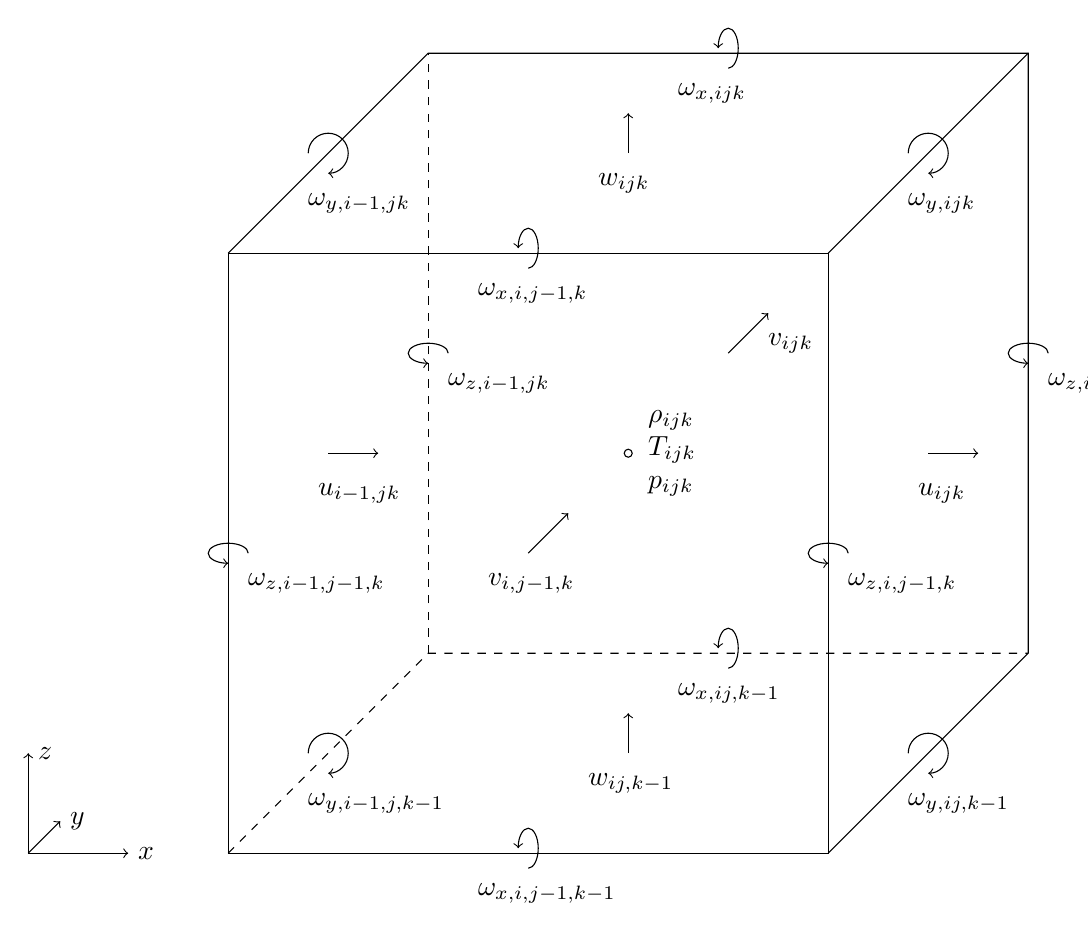
\begin{tikzpicture}[x=1in,y=1in]
\draw [->] (-1,0) -- (-0.5,0); \node[text width=1, anchor=west] at (-0.5,0) {$x$};
\draw [->] (-1,0) -- (-0.84,0.16); \node[text width=1, anchor=west] at (-0.84,0.16) {$y$};
\draw [->] (-1,0) -- (-1,0.5); \node[text width=1, anchor=west] at (-1,0.5) {$z$};
\draw (0,0) rectangle (3,3);
\draw (2,2) circle (0.02); \node[text width=1, anchor=west] at (2.05,2.0) {$\rho_{ijk}$ \\ $T_{ijk}$ \\ $p_{ijk}$ };
\draw (0,0) (3,0) -- (4,1) -- (4,4) -- (1,4) -- (0,3);
\draw (0,0) (3,3) -- (4,4);
\draw [dashed] (0,0) (0,0) -- (1,1) -- (4,1);
\draw [dashed] (0,0) (1,1) -- (1,4);
\draw [->] (0.5,2) -- (0.75,2); \node[text width=1, anchor=west] at (0.4,1.8) {$u_{i-1,jk}$};
\draw [->] (3.5,2) -- (3.75,2); \node[text width=1, anchor=west] at (3.4,1.8) {$u_{ijk}$};
\draw [->] (1.5,1.5) -- (1.7,1.7); \node[text width=1, anchor=west] at (1.25,1.35) {$v_{i,j-1,k}$};
\draw [->] (2.5,2.5) -- (2.7,2.7); \node[text width=1, anchor=west] at (2.65,2.55) {$v_{ijk}$};
\draw [->] (2.0,0.5) -- (2.0,0.7); \node[text width=1, anchor=west] at (1.75,0.35) {$w_{ij,k-1}$};
\draw [->] (2.0,3.5) -- (2.0,3.7); \node[text width=1, anchor=west] at (1.80,3.35) {$w_{ijk}$};
\draw [->] (0.4,3.5) arc (180:-90:.1); \node[text width=1, anchor=west] at (0.35,3.25) {$\omega_{y,i-1,jk}$};
\draw [->] (3.4,3.5) arc (180:-90:.1); \node[text width=1, anchor=west] at (3.35,3.25) {$\omega_{y,ijk}$};
\draw [->] (0.4,0.5) arc (180:-90:.1); \node[text width=1, anchor=west] at (0.35,0.25) {$\omega_{y,i-1,j,k-1}$};
\draw [->] (3.4,0.5) arc (180:-90:.1); \node[text width=1, anchor=west] at (3.35,0.25) {$\omega_{y,ij,k-1}$};
\draw [->] (1.5,-0.075) arc (-90:180:0.05 and 0.1); \node[text width=1, anchor=west] at (1.2,-0.2) {$\omega_{x,i,j-1,k-1}$};
\draw [->] (1.5, 2.925) arc (-90:180:0.05 and 0.1); \node[text width=1, anchor=west] at (1.2, 2.8) {$\omega_{x,i,j-1,k}$};
\draw [->] (2.5, 0.925) arc (-90:180:0.05 and 0.1); \node[text width=1, anchor=west] at (2.2, 0.8) {$\omega_{x,ij,k-1}$};
\draw [->] (2.5, 3.925) arc (-90:180:0.05 and 0.1); \node[text width=1, anchor=west] at (2.2, 3.8) {$\omega_{x,ijk}$};
\draw [->] (0.1, 1.5) arc (0:270:0.1 and 0.05); \node[text width=1, anchor=west] at (0.05, 1.35) {$\omega_{z,i-1,j-1,k}$};
\draw [->] (3.1, 1.5) arc (0:270:0.1 and 0.05); \node[text width=1, anchor=west] at (3.05, 1.35) {$\omega_{z,i,j-1,k}$};
\draw [->] (1.1, 2.5) arc (0:270:0.1 and 0.05); \node[text width=1, anchor=west] at (1.05, 2.35) {$\omega_{z,i-1,jk}$};
\draw [->] (4.1, 2.5) arc (0:270:0.1 and 0.05); \node[text width=1, anchor=west] at (4.05, 2.35) {$\omega_{z,ijk}$};
\end{tikzpicture}
\caption[Position of flow variables in a grid cell]{Position of flow variables in grid cell $ijk$. The arrows indicate the positive direction of the given variable. Scalar variables, such as the density, $\rho$, temperature, $T$, and pressure, $p$, are defined at the cell center. Velocity components, $\mathbf{u}=(u,v,w)$, are defined at their respective cell faces, and vorticity components, $\vec{\omega}=(\omega_x,\omega_y,\omega_z)$, are located at cell edges.}
\label{variable_positions}
\end{figure}

\section{Mass and Species Transport}
\label{sec_lumped_species}

The most basic description of the chemistry of fire is a reaction of a hydrocarbon fuel with oxygen that produces carbon dioxide and water vapor. Because fire is a relatively inefficient combustion process involving multiple fuel gases that contain more than just carbon and hydrogen atoms, the number of gas species to keep track of in the simulation is almost limitless. However, to make the simulations tractable, we limit the number of fuels to one, usually, and the number of reactions to just one or two. We also leave open the possibility that the reaction may not proceed for lack of sufficient oxygen in the incoming air stream, as when a fire in a closed compartment extinguishes itself. Even with this simplified approach to the chemistry, we still need to track at least six gas species (Fuel, O$_2$, CO$_2$, H$_2$O, CO, N$_2$) plus soot particulate. If we assume a single-step reaction, we do not need to solve explicitly seven transport equations. In fact, we only need to solve two -- one for the fuel and one for the products. The air is everything that is neither fuel nor products. However, to ensure realizability of species mass fractions, our strategy is to solve a transport equation for each species mass density and then to obtain the mixture mass density by summation of the species densities.

Whereas the fuel is usually a single gas species, the air and products are what are often referred to as ``lumped species''. A lumped species represents a mixture of gas species that transport together (i.e., the lumped species has a single set of transport properties) and react together, and from the point of view of the numerical model, a lumped species can be treated as a single species. In fact, the mass transport equations make no distinction between a single or lumped species. For example, air is a lumped species that consists of nitrogen, oxygen, and trace amounts of water vapor and carbon dioxide. We use the symbols $Z_A$, $Z_F$, and $Z_P$ to denote the mass fractions of air, fuel and products.  The lumped species mass fractions are linearly related to the primitive species mass fractions, $Y_\alpha$; thus, conversion from one to the other is a simple matter of performing a matrix multiplication.  For example, the complete combustion of methane:
\be \mathrm{CH_4 + 2 \, \left( O_2 + 3.76 \, N_2 \right)  \rightarrow CO_2 +2 \, H_2O + 7.52 \, N_2} \ee
is expressed as
\be \hbox{Fuel} + 2 \, \hbox{Air} \rightarrow \hbox{Products} \ee
and the primitive species can be recovered from the lumped species via
\be \left[ \begin{array} {c c c}
0.77 & 0.00 & 0.73 \\
0.23 & 0.00 & 0.00 \\
0.00 & 1.00 & 0.00 \\
0.00 & 0.00 & 0.15 \\
0.00 & 0.00 & 0.12  \end{array}
\right]
\left[ \begin{array} {c} Z_{\rm A} \\ Z_{\rm F} \\ Z_{\rm P} \end{array} \right] =
\left[ \begin{array} {c} Y_\NTWO \\ Y_\OTWO \\ Y_{\scriptscriptstyle \mathrm{CH_4}} \\ Y_\COTWO \\ Y_{\scriptscriptstyle \mathrm{H_2O}} \end{array} \right]
 \ee
Notice that the columns of the matrix are the mass fractions of the primitive species within a given lumped species.

The transport equation for each of the lumped species has the same form as the transport equation for a single species:
\be \dod{ }{t}(\rho Z_\alpha) + \nabla\!\cdot (\rho Z_\alpha \bu) = \nabla\!\cdot (\rho D_\alpha \nabla Z_\alpha) + \dm_\alpha''' + \dm_{\rm b,\alpha}''' \label{species} \ee
Note that the source term on the right hand side represents the addition of mass from evaporating droplets or other subgrid-scale
particles that represent sprinkler and fuel sprays, vegetation, and any other type of small, unresolvable object. These
objects are assumed to occupy no volume; thus they are seen by the governing equations as point sources of mass, momentum, and energy. It is important to
note, however, that the evaporated mass species must be one for which an explicit transport equation is solved. For example, water vapor is a product of
combustion, but it is also formed by evaporating sprinkler droplets. In cases such as these, there needs to be an explicit transport equation for water
vapor to distinguish between that which is formed by combustion and that which is evaporated from the droplets. Here $\dm_{\rm b,\alpha}'''$ is the production rate of species $\alpha$ by evaporating droplets or particles.

The mass density is obtained from $\rho = \sum (\rho Z)_\alpha$.  The summation of Eq.~(\ref{species}) over all $N_s$ species gives
\be \dod{\rho}{t} + \nabla\!\cdot (\rho \bu)  =  \dm_{\rm b}'''  \label{mass} \ee
because $\sum Z_\alpha=1$ and $\sum \dm_\alpha''' = 0$ and $\sum \dm_{\rm b,\alpha}'''=\dm_{\rm b}'''$, by definition, and because it is assumed that $\sum \rho D_\alpha \nabla Z_\alpha = 0$. This last assertion is not true, in general.  The diffusive flux for the most abundant local species is corrected to enforce the constraint.




\paragraph{Enforcing Realizability} ~\\

\noindent Realizability of species mass fractions requires $Y_\alpha \ge 0$ for all $\alpha$ and $\sum Y_\alpha = 1$.  Note that this is more restrictive than the boundedness constraint, which simply requires $0 \le Y_\alpha \le 1$.

If $(\rho Y)_\alpha$ obeys boundedness, $(\rho Y)_\alpha \ge 0$, and we solve $N_s$ species equations obtaining the density via $\rho = \sum_{\alpha=1}^{N_s} (\rho Y)_\alpha$, then mass fractions obtained by $Y_\alpha = (\rho Y)_\alpha/\rho$ are \emph{guaranteed to be realizable} (for $\rho>0$).  Thus, we have reduced the realizability problem to the ``easier'' problem of boundedness for $(\rho Y)_\alpha$. Details of the scalar boundedness correction are discussed in Appendix \ref{app_boundedness}.

With this approach we must take care to ensure $\sum \rho D_\alpha \nabla Z_\alpha = 0$.  Our strategy is to absorb any errors in diffusive transport into the most abundant species \emph{locally}.  That is, for a given cell face we set $\rho D_m \nabla Z_m = -\sum_{\alpha\ne m} \rho D_\alpha \nabla Z_\alpha$, where $m$ is the most abundant species adjacent to that face.  Note that since FDS is typically used as an LES code mass transport by molecular diffusion may be two or three orders of magnitude less than turbulent transport, which uses the same turbulent diffusion coefficient for all species. Therefore, the errors in summation of the diffusive fluxes tend to be small.

\section{Low Mach Number Approximation}

Rehm and Baum~\cite{Rehm:1} observed that for low speed applications like fire, the spatially and temporally resolved pressure, $p$, can be decomposed into a ``background'' pressure, $\bp(z,t)$, plus a perturbation, $\tp(x,y,z,t)$, with only the background pressure retained in the equation of state (ideal gas law):
\be \bp = \rho T \R \sum_\alpha  \frac{Z_\alpha}{W_\alpha} \equiv \frac{\rho \R T}{\bW}  \label{basicstate1} \ee
Note that $z$ is the spatial coordinate in the direction of gravity; thus, the stratification of the atmosphere is included in the background pressure. The perturbation, $\tp$, drives the fluid motion. This approximation has a number of consequences. First, building compartments connected via a heating, ventilation, and air conditioning (HVAC) system can each maintain individual background pressures. The air flows between compartments can be
described in terms of the differences in the background pressures, eliminating the need to solve detailed flow equations within the ventilation ducts.

The second consequence of the low Mach number approximation is that the internal energy, $e$, and enthalpy, $h$, may be related in terms of the thermodynamic (background) pressure: $h = e + \bp/\rho$.  The energy conservation equation may then be written in terms of the {\em sensible enthalpy}, $h_{\rm s}$:
\be \dod{ }{t}(\rho h_{\rm s}) + \nabla\!\cdot (\rho h_{\rm s} \bu) = \DoD{\bp}{t} + \dq''' + \dq_{\rm b}''' - \nabla\!\cdot \dbq'' \label{energy} 
\ee
The term $\dq'''$ is the heat release rate per unit volume from a chemical reaction. The term $\dq_{\rm b}'''$ is the energy transferred to subgrid-scale droplets and particles. The term $\dbq''$ represents the conductive, diffusive, and radiative heat fluxes:
\be
   \dbq'' = -k \nabla T - \sum_\alpha h_{\rm s,\alpha} \, \rho \, D_\alpha \nabla Z_\alpha + \dbq_{\rm r}''  \label{bqdot_def}
\ee
where $k$ is the thermal conductivity and $D_\alpha$ is the diffusivity of species $\alpha$.

Eq.~(\ref{energy}) is not solved explicitly. Instead, the velocity divergence is factored out as follows:
\be
\label{eqn_simplediv1}
\Div\mathbf{u} = \frac{1}{\rho h_{\rm s}} \left[ \DoD{}{t} (\bp-\rho h_{\rm s}) + \dq''' + \dq_{\rm b}^\ppp - \Div \dot{\mathbf{q}}^\pp \right]
\ee
The hydrodynamics solver guarantees that Eq.~(\ref{eqn_simplediv1}) is satisfied.  It follows that Eq.~(\ref{energy}) is also satisfied (energy is conserved).

Expanding the material derivatives on the right hand side of Eq.~(\ref{eqn_simplediv1}) produces a fairly complicated expression for
the divergence that includes the source and diffusion terms from the mass, species, and energy conservation equations. Its importance to the overall algorithm is that it can be computed using only the thermodynamic variables $\rho$, $Z_\alpha$, and $\bp$. As will be shown below, the way to advance the flow velocity in time is to first estimate the thermodynamic variables at the next time step, compute the divergence, and then solve an equation for the pressure that will guarantee that the divergence of the updated velocity is identical to that computed solely from the thermodynamic variables.



\section{Momentum Transport}

Noting the vector identity $(\bu \cdot \nabla) \bu = \nabla|\bu|^2/2 - \bu\times\bo $, and defining the stagnation energy per unit mass, $\cH \equiv |\bu|^2/2 + \tp/\rho$, the momentum equation can be written (see Chapter \ref{momentum_chapter} for a detailed derivation)
\be
   \dod{\bu}{t} - \bu\times\bo + \nabla \cH - \tp \, \nabla \left( 1/\rho\right) = \frac{1}{\rho} \Big[ (\rho-\rho_0) \bg + \bof_{\rm b} + \nabla\!\cdot \btau \Big] \label{momeqnoncon}
\ee
The term $\bof_\text{b}$ represents the drag force exerted by the subgrid-scale particles and droplets. The viscous stress, $\btau$, is closed via gradient diffusion with the turbulent viscosity obtained from the Deardorff eddy viscosity model \cite{Deardorff:1980,Pope:2000}. It is convenient to write Eq.~(\ref{momeqnoncon}) in the form:
\be
   \dod{\bu}{t} + \bF + \nabla \cH  = 0
\ee
so that a Poisson equation for the pressure can be derived by taking its divergence:
\be
   \nabla^2 \cH = - \left[ \dod{ }{t} (\nabla\!\cdot \bu) + \nabla\!\cdot \bF  \right]   \label{simplephi2}
\ee
Note the appearance of the time derivative of the divergence. This is an important feature of the time marching scheme. Note also that the right hand side of the Poisson equation retains a term that includes the perturbation pressure, $\tp \, \nabla (1/\rho)$. This term accounts for the baroclinic torque. It is included on the right hand side of the Poisson equation by using its value from the previous time step. This approximation allows us to solve a separable form of the Poisson equation, for which there are fast, direct solvers that are optimized for uniform grids~\cite{Sweet:1}.

\section{Combustion and Radiation}

FDS is described as a ``fire model'' because it incorporates source terms and boundary conditions that describe the
turbulent combustion of gaseous fuel and oxygen, the transport of thermal radiation through hot, soot-laden gases, the
thermal decomposition of real materials, the activation of sprinklers and smoke detectors, the transport of water and liquid fuel
droplets, and a variety of other features that describe fires inside and outside of buildings.

Combustion and radiation are introduced into the governing equations via the source terms, $\dq^\ppp$ and $\dq_{\rm r}^\ppp$,
in the energy transport equation. Since the energy equation is not solved explicitly, these terms find their way into the
expression for the divergence.

\subsection{Combustion}

For most applications, FDS uses a combustion model based on the mixing-limited, infinitely fast reaction of lumped species.
Lumped species are reacting scalar quantities that represent a mixture of species.  For example, air is a lumped species which is a mixture of
nitrogen, oxygen, water vapor, and carbon dioxide.  The reaction of fuel and oxygen is not necessarily instantaneous and
complete, and there are several optional schemes that are designed to predict the extent of combustion in under-ventilated spaces.

For an infinitely-fast reaction, reactant species in a given grid cell are converted to product species at a rate determined by a
characteristic mixing time, $\tau_{\rm mix}$. The heat release rate per unit volume is defined by summing the lumped species mass production rates times their respective heats of formation
\be
   \dq''' = -\sum_\alpha \dm_\alpha''' \, \Delta h_{\rm f,\alpha} \label{EDC1}
\ee  %Y rather than Z is correct in this equation
Details of $\tau_{\rm mix}$ and $\dm_\alpha'''$ are discussed in Chapter \ref{combustionsection}.

\subsection{Radiation}

The net contribution from thermal radiation in the energy equation is defined by:
\be
    \dq_r^\ppp \equiv -\nabla\!\cdot \dbq_{\rm r}''(\bx) =
    \kappa(\bx) \, \left[ U(\bx) - 4 \pi \, I_{\rm b}(\bx) \right]  \quad ; \quad
    U(\bx) = \int_{4\pi} \, I(\bx,\bs') \, d\bs'  \label{simple_rte}
\ee
where $\kappa(\bx)$ is the absorption coefficient, $I_b(\bx)$ is the source term, and $I(\bx,\bs)$ is the solution of the radiation transport equation (RTE) for a non-scattering gray gas:
\be
   \bs \cdot \nabla I(\bx,\bs) = \kappa(\bx) \; \left[ I_{\rm b}(\bx) - I(\bx,\bs) \right] \label{bandRTE1}
\ee
In practical simulations, the spectral dependence of $I$, $I_b$, and $\kappa$ cannot be resolved accurately, nor do we have reliable data for non-ideal fuels typical of real fires. While FDS does have an option to divide the radiation spectrum into a relatively small number of bands and solve a separate RTE for each band, it is usually not necessary because in real fires, soot is the dominant source and sink of thermal radiation and is not particularly sensitive to wavelength. The mean absorption coefficient, $\kappa$, is a function of species composition and temperature. Its values are obtained from a narrow-band model called RadCal~\cite{RadCal}.

The source term, $I_{\rm b}$, requires special treatment because of the limited resolution of the underlying numerical grid in the vicinity of flames. In large scale fire simulations, grid cells are typically on the order of
tens of centimeters. Flame sheets cannot be resolved, meaning that the computed cell-average temperature can be significantly lower than temperatures one would expect to find in the reacting flame. Consequently, the
source term is approximated in grid cells where fuel and oxygen react. Elsewhere, the subgrid temperature field is homogeneous and the source term can be computed directly:
\be \kappa \; I_{\rm b} = \left\{ \begin{array}{cll}
    \kappa \, \sigma \, T^4/\pi      & \hbox{Outside flame zone}, & \dot{q}'''=0  \\ [0.1in]
    C\, \kappa \, \sigma \, T^4/\pi  & \hbox{Inside flame zone}, & \dot{q}'''>0
    \end{array} \right.  \label{radapprox1}
\ee
The constant $C$ is computed at each time step so that the volume integral of Eq.~(\ref{simple_rte}) over the entire flaming region is approximately equal to the volume integral of $\chi_{\rm r} \,\dot{q}'''$ over that same region. Here, $\chi_{\rm r}$ is an empirical estimate of the {\em global} fraction of that energy emitted as thermal radiation. Typically, a sooty fire radiates approximately one-third of the total combustion energy.

The radiation equation is solved using a technique similar to a finite volume method for convective transport, thus the name given to it is the Finite Volume Method (FVM). Using approximately 100 discrete angles which are updated over multiple time steps, the finite volume solver requires about 20\% of the total CPU time of a calculation, a modest cost given the complexity of radiation heat transfer.

Water droplets can absorb and scatter thermal radiation. This is important in scenarios involving water mist suppression systems, but also plays a role in all sprinkler cases. The absorption and scattering coefficients are based on Mie theory. The scattering from the gaseous species and soot is considered negligible and is not included in the model.



\section{Solution Procedure}
\label{sec:solution_procedure}

In a given grid cell at the $n$th time step, we have the density, $\rho^n$, lumped species mass fractions, $Z_\alpha^n$, velocity
vector, $\bu^n$, and the Bernoulli integral, $\cH^n$.
In addition, for each compartment in the computational domain, we have a background pressure, $\bp^n$. The temperature is
found from the equation of state. These variables are advanced in time using an explicit second-order predictor/corrector scheme.
The basic procedure is as follows:

\paragraph{Predictor}

\begin{enumerate}
\item Estimate $\rho$, $Z_\alpha$, and $\bp$ at the next time step with an explicit Euler step. The species mass density is estimated by
\be \frac{(\rho Z)_\alpha^*- \rho^n Z_\alpha^n}{\dt} + \nabla\!\cdot \rho^n \, Z_\alpha^n \, \bu^n = \nabla\!\cdot (\rho^n D_\alpha^n \nabla Z_\alpha^n) + (\dot{m}_\alpha''' + \dot{m}_{\rm b,\alpha}''')^n \ee
The asterisk denotes a first order accurate estimate at the next time step. Note that the mass source terms are computed in the previous time step using the corrected value of the density and species mass fractions.

\item Compute the density from $\rho^* = \sum_\alpha (\rho Z_\alpha)^*$ and mass fractions from $Z_\alpha^* = (\rho Z)_\alpha^*/\rho^*$.

\item Compute the temperature, $T^*$, from the equation of state.

\item \label{step_pred_div} Compute the divergence, $(\nabla\!\cdot \bu)^*$, from Eq.~(\ref{eqn_simplediv1}) using the estimated thermodynamic quantities. Note that we use the parentheses to emphasize that an estimate of the velocity field, $\bu^*$, at the next time step has not been computed yet, only its divergence.

\item Solve the Poisson equation for the pressure term:
\be \nabla^2 \cH^n = - \frac{ (\nabla\!\cdot \bu)^* - \nabla\!\cdot \bu^n }{\dt} - \nabla\!\cdot \bF^n  \ee

\item Estimate the velocity at the next time step.
\be
\frac{\bu^* - \bu^n}{\dt} +  \bF^n + \nabla \cH^n  = 0
\ee
Note that this procedure guarantees that the divergence of the estimated velocity field, $\nabla\!\cdot \bu^*$, is identically
equal to the divergence that is derived from the estimated thermodynamic quantities, $(\nabla\!\cdot \bu)^*$, in Step \ref{step_pred_div}.

\item Check that the time step, $\dt$, satisfies the stability condition (see Sec.~\ref{stability}).
If the time step is too large, it is reduced so that it satisfies
the stability constraint and the procedure returns to the beginning of the time step.
If the stability criterion is satisfied, the procedure continues to the corrector step.
\end{enumerate}

\paragraph{Corrector}

\begin{enumerate}

\item Correct the transported species mass densities at the next time step.
\be
\frac{(\rho Z_\alpha)^{n+1} - \ha \left(\rho^n Z_\alpha^n + \rho^* Z_\alpha^* \right)}{\dt/2} +  \nabla\!\cdot \rho^* Z_\alpha^* \bu^* =
\nabla\!\cdot (\rho^* D_\alpha^* \nabla Z_\alpha^*) + (\dot{m}_\alpha'''+ \dot{m}_{\rm b,\alpha}''')^n
\ee
The background pressure is corrected similarly. Note that the mass source terms are the same as those added in the predictor step. They are only computed once per time step.

\item Compute the density $\rho^{n+1} = \sum_\alpha (\rho Z_\alpha)^{n+1}$ and mass fractions $Z_\alpha^{n+1} = (\rho Z_\alpha)^{n+1}/\rho^{n+1}$.

\item Compute the temperature, $T^{n+1}$, from the equation of state.

\item \emph{Time splitting for mass source terms}. After the corrector step for the transport scheme, source terms are computed and stored.  The source terms are evaluated using the results from the corrected scalar transport scheme. The source terms include the heat release rate per unit volume, $\dot{q}'''$, the net absorption/emittance of thermal radiation, $\nabla \cdot \dot{\bq}''$, and the mass species source terms, $\dot{m}_\alpha'''$. In addition, the terms in the divergence expression, Eq.~(\ref{eqn_div_1}), involving the source terms are computed and stored. All of these quantities are computed at this point in the time step and applied in both the predictor and corrector steps of the following time step.

\item \label{step_cor_div} Compute the divergence, $(\nabla\!\cdot \bu)^{n+1}$, from the corrected thermodynamic quantities.

\item Compute the pressure using the estimated quantities.
\be
\label{eqn_corrector_poisson2}
\nabla^2\cH^* = - \left[ \frac{ (\nabla\cdot\bu)^{n+1} - \ha \left( \nabla\cdot \bu^* + \nabla\cdot \bu^n \right) }{\dt/2} \right] - \nabla\!\cdot \mathbf{F}^*
\ee

\item Correct the velocity at the next time step.
\be
\frac{ \bu^{n+1} - \ha \left( \bu^* + \bu^n \right)}{\dt/2} + \mathbf{F}^* + \nabla \cH^* = 0
\ee
Note again that the divergence of the corrected velocity field is identically equal to the divergence that was computed in Step \ref{step_cor_div}.


\end{enumerate}

% !TEX root = FDS_Technical_Reference_Guide.tex

\typeout{new file: Mass_Chapter.tex}

\chapter{Mass, Species, and Enthalpy Transport}

This chapter describes in detail the equation of state in the low Mach number limit, the finite difference approximation of the mass and species conservation equations, and the role of the flow divergence as a surrogate for the enthalpy transport equation.
Due to the use of the low Mach number approximation, the energy conservation equation is not solved explicitly but rather is defined implicitly via the divergence of the flow field, which contains the combustion and radiation source terms.


\section{The Equation of State}

A distinguishing feature of a CFD model is the regime of
flow speeds (relative to the speed of sound) for which it is designed. High
speed flow codes involve compressibility effects and shock waves. Low speed
solvers, however, explicitly eliminate compressibility effects that give rise
to acoustic (sound) waves. The Navier-Stokes equations describe the
propagation of information at speeds comparable to that of the fluid flow (for fire, approximately \SI{10}{m/s}),
but also at speeds comparable to that of sound waves (for still air,
\SI{300}{m/s}). Solving a discretized form of these equations would require extremely small
time steps in order to account for information traveling at the speed of sound, making
practical simulations difficult.

Following the work of Rehm and Baum~\cite{Rehm:1}, an approximation to the equation of state is made by decomposing the pressure
into a ``background'' component and a perturbation. It is assumed that
the background component of pressure can differ from compartment to compartment. If
a volume within the computational domain is isolated from other volumes, except via leak paths or ventilation ducts, it is referred to as a ``pressure zone'' and assigned its own background pressure. The pressure field within the $m$th zone, for example, is a linear combination
of its background component and the flow-induced perturbation:
\be
   p(\bx,t) = \bp_m(z,t) + \tp(\bx,t)
\ee
Note that the background pressure is a function of $z$, the vertical spatial coordinate, and the time, $t$. For most compartment fire applications, $\bp_m$ changes very little with height or time. However, for scenarios where a fire increases the pressure in a closed compartment, or where the HVAC system affects the pressure, or when the height of the domain is significant, $\bp_m$ takes these effects into account~\cite{Baum:5}. The ambient pressure field is denoted $\bp_0(z)$. Note that the subscript 0 denotes the exterior of the computational domain, not time 0. This is the assumed atmospheric pressure stratification that serves as both the initial and boundary condition for the governing equations.

The purpose of decomposing the pressure is that for low Mach number flows, it can be assumed that the temperature and density are inversely proportional, and thus the equation of state (in the $m$th pressure zone) can be approximated as
\be
   \bp_m  =  \rho T \R \sum_\alpha \frac{Z_\alpha}{W_\alpha} = \frac{\rho T \R}{ \bW }  \label{state}
\ee
Recall from Section~\ref{sec_lumped_species} that $Z_\alpha$ is the mass fraction of lumped species $\alpha$. The pressure, $p$, in the state and energy equations is replaced by the background pressure $\bp_m$ to filter out sound waves that travel at speeds that are much faster than typical flow speeds expected in fire applications. The low Mach number assumption serves two purposes. First, the filtering of acoustic waves means that the time step in the numerical algorithm is bound only by the flow speed as opposed to the speed of sound, and second, the modified state equation leads to a reduction in the number of dependent variables in the system of equations by one. The energy equation (\ref{energy}) is not explicitly solved; rather, its source terms are included in the expression for the flow divergence, to be discussed later in the chapter.  When the velocity field satisfies the specified thermodynamic divergence, the conservative form of the sensible enthalpy equation is satisfied by construction.

The stratification of the atmosphere is derived from the relation
\be \frac{\d \bp_0}{\d z} = - \rho_0(z) \, g  \ee
where $\rho_0$ is the background density and $g=\SI{9.8}{m/s}$. Using Eq.~(\ref{state}), the background pressure can be written as a function of the background temperature, $T_0(z)$,
\be \bp_0(z) = p_\infty \; \exp \, \left( -\int^z_{z_\infty} \frac{\bW \, g}{\R \, T_0(z')} \d z' \right)  \label{pstrat} \ee
where the subscript infinity generally refers to the ground. A linear temperature stratification of the atmosphere may be
specified by the user such that $T_0(z) = T_\infty + \Gamma z$ where $T_\infty$ is the temperature at the ground and
$\Gamma$ is the lapse rate (e.g., $\Gamma = -\SI{0.0098}{K/m}$ is the {\em adiabatic lapse rate}).
In this case $\bp_0$ and $\rho_0$ are derived from Eqs.~(\ref{pstrat}) and (\ref{state}), respectively.
It can then be shown that for $\Gamma \ne 0$ the pressure stratification becomes
\be
   \bp_0(z) = p_\infty  \left( \frac{T_0(z)}{T_\infty} \right)^{\overline{W}g/\R \Gamma}
   \label{pstrat2}
\ee


\section{Mass and Species Transport}

The species transport equations are solved using a predictor-corrector scheme. Advection terms are written in flux divergence (conservative) form. In the predictor step, the mass density in cell $ijk$ at time level $n+1$ is estimated based on information at the $n$th level:
\be  \frac{(\rho Z_\alpha)_{ijk}^{*}-(\rho Z_\alpha)_{ijk}^n}{\dt}
  + \nabla\!\cdot(\overline{\rho Z_\alpha}^{\rm FL} \mathbf{u})_{ijk}^n
  = \nabla\!\cdot (\rho D_\alpha \nabla Z_\alpha)_{ijk}^n + \left( \dot{m}'''_\alpha + \dot{m}'''_{\rm b,\alpha} \right)_{ijk}^n
\ee
The quantity $\overline{\rho Z_\alpha}^{\rm FL}$ indicates a \emph{flux limiter} applied to the cell face value, as discussed below in Section \ref{sec_flux_limiters}. The mass source terms due to chemistry, evaporation, or pyrolysis are computed at the end of the previous time step and used in both the predictor and corrector steps. The mean chemical source term, $\dm_{\alpha}'''$, is discussed in Chapter~\ref{combustionsection}.  The bulk subgrid source term, $\dm_{\rm b,\alpha}'''$, is discussed in Chapters~\ref{chapter:solid_phase} and \ref{chapter:lagrangian_particles} on solid phase pyrolysis and Lagrangian particles, respectively.

In DNS mode, the molecular diffusivity is based on mixture-averaged binary Fickian diffusion.  In LES mode (default) the diffusivity is taken from the molecular and turbulent viscosities divided by the turbulent Schmidt number.  That is, to save cost we approximate the molecular plus turbulent diffusivity by $(\mu + \mu_t)/\mbox{Sc}_t$.   The turbulent Schmidt number is constant with default value $\mbox{Sc}_t = 0.5$.  The model for the turbulent viscosity $\mu_t$ is discussed in Section \ref{section:turbulent_viscosity}.  Optionally, by setting \textct{SIMULATION\_MODE='LES'} on \textct{MISC}, the molecular and turbulent transport coefficients are treated separately, $\rho D_\alpha + \mu_t/\mbox{Sc}_t$ (at added cost).  The same applies for the thermal diffusivity.

The corrector step is as follows:
\be \frac{(\rho Z_\alpha)_{ijk}^{n+1}-\ha\left[(\rho Z_\alpha)_{ijk}^n
    +(\rho Z_\alpha)_{ijk}^{*}\right]} {\ha \dt}
    + \nabla\!\cdot(\overline{\rho Z_\alpha}^{\rm FL} \mathbf{u})_{ijk}^*
    = \nabla\!\cdot (\rho D_\alpha \nabla Z_\alpha)_{ijk}^{*} + \left( \dot{m}'''_\alpha + \dot{m}'''_{\rm b,\alpha} \right)_{ijk}^n
\ee


\subsection{Flux Limiters}
\label{sec_flux_limiters}

A \emph{flux limiter} is an interpolation scheme for defining mass fluxes at cell faces. Simple linear interpolation of the cell-centered scalar variables to the cell face would result in a central difference scheme.  Such purely centered schemes are known to generate intolerable levels of dispersion error (spurious wiggles) leading to unphysical results such as negative densities or mass fractions outside the range of [0,1].  To address this issue, FDS relies on two schemes: a \emph{flux limiter} (discussed below) that handles the bulk of the problem, and a \emph{flux correction} (see Appendix~\ref{app_boundedness}) that adds the minimum amount of numerical diffusion to maintain boundedness.

For uniform flow velocity, a fundamental property of the exact solution to the equations governing scalar transport is that the total variation of the scalar field (the sum of the absolute values of the scalar differences between neighboring cells) is either preserved or diminished (never increased).  In other words, no new extrema are created.  Numerical schemes which preserve this property are referred to as total variation diminishing (TVD) schemes.  The practical importance of using a TVD scheme for fire modelling is that such a scheme is able to accurately track coherent vortex structure in turbulent flames and does not develop spurious reaction zones.

FDS employs two second-order TVD schemes as options for scalar transport: Superbee and CHARM.  Superbee \cite{Roe:1986} is recommended for LES because it more accurately preserves the scalar variance for coarse grid solutions that are not expected to be smooth.  Due to the gradient steepening applied in Superbee, however, the convergence degrades at small grid spacing for smooth solutions (the method will revert to a stair-step pattern instead of the exact solution).  CHARM \cite{Zhou:1995}, though slightly more dissipative than Superbee, is convergent, and is therefore the better choice for DNS calculations where the flame front is well resolved.

To illustrate how flux limiters are applied to the scalar transport equations, below we discretize the advection terms in Eq.~(\ref{species}) in one dimension:
\be  \frac{(\rho Z)_{i}^* - (\rho Z)_{i}^n}{\dt}
    + \frac{\overline{\rho Z}^{\rm FL}_{i+\frac{1}{2}} u_{i+\frac{1}{2}} - \overline{\rho Z}^{\rm FL}_{i-\frac{1}{2}} u_{i-\frac{1}{2}}}{\dx} = ...
\ee
Note that the $\pm\ha$ suffixes indicates a face value for a particular cell $i$. A flux-limited scalar value (density in this case) premultiplies the staggered, face-centered velocity to form the scalar advective flux.  Recall that these velocity values are primitive variables in the calculation---they are \emph{not} interpolated.
Consider face $i+\frac{1}{2}$ between cells $i$ and $i+1$ and let $\phi$ denote a general scalar variable, like $\rho Z_\alpha$.  The local (loc) and upstream (up) data variations are
\begin{align}
\delta \phi_{\rm loc} &= \phi_{i+1}-\phi_i \\
\delta \phi_{\rm up}  &= \left\{ \begin{array}{ll} \phi_i-\phi_{i-1} & \mbox{if} \quad u_i>0 \\ \phi_{i+2}-\phi_{i+1} & \mbox{if} \quad u_i<0 \end{array} \right.
\end{align}
The limiter function $B(r)$ depends on the upstream-to-local data ratio, $r=\delta \phi_{\rm up}/\delta \phi_{\rm loc}$. In FDS, options for the limiter function include \cite{Toro}:
\begin{table}[H]
\begin{center}
\begin{tabular}{lc}
Flux Limiter                           & $B(r)$                         \\
\hline
Central Difference                     & 1                              \\
Godunov                                & 0                              \\
MINMOD                                 & $\max(0,\min(1,r))$            \\
Superbee \cite{Roe:1986} (LES default) & $\max(0,\min(2r,1),\min(r,2))$ \\
CHARM \cite{Zhou:1995} (DNS default)   & $s(3s+1)/(s+1)^2$; $s=1/r$     \\
MP5 \cite{Suresh:1997}                 & see below
\end{tabular}
\end{center}
\end{table}
\noindent For the Central Difference, Godunov, MINMOD, and Superbee limiters, the scalar face value is found from
\begin{equation}
\label{eqn_flux_limiter}
\overline{\phi}^{\rm FL}_{i+1/2} = \left\{ \begin{array}{lcll} \phi_i &+& B(r) \,\frac{1}{2} \,\delta \phi_{\rm loc} & \mbox{if} \quad u_i>0 \vspace{0.2 cm}\\
\phi_{i+1} &-& B(r) \,\frac{1}{2} \,\delta \phi_{\rm loc} & \mbox{if} \quad u_i<0 \end{array} \right.
\end{equation}
For CHARM, the face value is given by~\cite{Kempf:2003}
\begin{equation}
\label{eqn_charm_limiter}
\overline{\phi}^{\rm FL}_{i+1/2} = \left\{ \begin{array}{lcll} \phi_i &+& B(r) \,\frac{1}{2} \,\delta \phi_{\rm up} & \mbox{if} \quad u_i>0 \vspace{0.2 cm}\\
\phi_{i+1} &-& B(r) \,\frac{1}{2} \,\delta \phi_{\rm up} & \mbox{if} \quad u_i<0 \end{array} \right.
\end{equation}
The MP5 scheme of Suresh and Huynh \cite{Suresh:1997} is based on the keen observation that three points cannot distinguish between extrema and discontinuities.  The functional form of the limiter is not as simple as the three-point schemes described above, so we refer the reader to the original paper or the FDS source code for details.  But the basic idea behind the method is to use a five-point stencil, three upwind and two downwind, to reconstruct the cell face value, considering both accuracy and monotonicity-preserving constraints.  An additional benefit of the MP5 scheme is that it was designed specifically with strong stability-preserving (SSP) Runge-Kutta time discretizations in mind.  The predictor-corrector scheme used by FDS is similar to the second-order SSP scheme described in \cite{Gottlieb:2001}.


\subsubsection{Notes on Implementation}

In practice, we set $r=0$ initially and only compute $r$ if the denominator is not zero.  Note that for $\delta \phi_{loc}=0$, it does not matter which limiter is used: all the limiters yield the same scalar face value.  For CHARM, we set both $r=0$ and $B=0$ initially and only compute $B$ if $r>0$ (this requires data variations to have the same sign). Otherwise, CHARM reduces to Godunov's scheme.

The Central Difference, Godunov, and MINMOD limiters are included for completeness, debugging, and educational purposes.  These schemes have little utility for typical FDS applications.

\subsection{Time Splitting for Mass Source Terms}
\label{sec_time_splitting}

Following the corrector step of the transport scheme, source terms are computed for the next time step.  The source terms are typically related to particle evaporation or combustion, and these processes are computed at the end of the time step. In the case of combustion, the total mass of a grid cell is not changed; rather the species mass fractions change. The mean chemical source term, $\dm_{\alpha}'''$, is discussed in Chapter~\ref{combustionsection}.  The bulk subgrid source term, $\dm_{\rm b,\alpha}'''$, is discussed in Chapters~\ref{chapter:solid_phase} and \ref{chapter:lagrangian_particles} on solid phase pyrolysis and Lagrangian particles, respectively.


\subsection{Boundary Conditions for Temperature, Species Mass Fraction, and Density}
\label{section:TZD_bc}

The gas temperature, species mass fractions, and density are computed at the center of each grid cell. At an exterior boundary, or at
the boundary of an interior obstruction, these values must be computed at the face of the cell that falls at the boundary interface. In general, the temperature at the boundary, $T_{\rm w}$, is computed first, followed by species mass fractions, $Z_{\rm \alpha,w}$, followed by density, $\rho_{\rm w}$. The density is typically determined from the equation of state:
\be  \rho_{\rm w} = \frac{\overline{p}_m}{ \R \, T_{\rm w} \, \sum_\alpha (Z_{\rm \alpha,w}/W_\alpha) }  \ee
Here, $\overline{p}_m$ denotes the background pressure of the gas phase region.

When necessary, the boundary value is linearly extrapolated one half of a grid cell into the ``ghost'' cell for use by the gas phase solver. In the sections below, the value at the center of the gas phase cell adjacent to the boundary is denoted with the subscript ``g'' (for ``gas phase'', \emph{not} ``ghost''), and the value at the boundary by ``w'' (for ``wall'').

\subsubsection{Solid Boundaries}

At a solid boundary, the surface temperature, $T_{\rm w}$, is either specified or computed as described in Chapter~\ref{chapter:solid_phase}. For an LES calculation, the convective heat flux at the surface is determined via an empirical heat transfer coefficient, $h$, and the convective heat flux at the boundary is written:
\be
   k \frac{T_{\rm g} - T_{\rm w}}{\dn/2} = h \; (T_{\rm g}-T_{\rm w})  \label{ebal}
\ee
where $\dn/2$ is the distance between the surface and the center of the adjacent gas phase cell. The convective heat transfer coefficient, $h$, is described in Section~\ref{conflux}. For a DNS calculation, the convective heat transfer is determined directly from the computed or specified surface temperature.

There is no transfer of mass at a solid boundary; thus, the boundary value for the species mixture $\alpha$ is simply
\be Z_{\rm \alpha,w} = Z_{\rm \alpha,g} \ee

\subsubsection{Open Boundaries}

The term ``open'' denotes a non-solid exterior boundary of the computational domain. Gases are allowed to flow freely in and out. At these boundaries, the temperature and species mass fractions take on their respective exterior values if the flow is incoming, and take on their respective values in the grid cell adjacent to the boundary if the flow is outgoing. This is a simple upwind boundary condition.



\subsubsection{Specified Mass Flux}

Here, the mass flux of species $\alpha$, $\dot{m}_\alpha''$, is specified or computed as part of the overall solid phase calculation. To determine the mass fraction of species mixture $\alpha$ at the boundary, $Z_{\alpha,f}$, the following equations must be solved iteratively
\begin{gather}
\label{eqn_total_mass_flux} \sum_\alpha \dot{m}_\alpha'' = \rho_{\rm w} u_n \\
\label{eqn_spec_mass_flux}  \dot{m}_\alpha'' = u_n \rho_{\rm w} Z_{\rm \alpha,w} - (\rho D_\alpha)_{\rm w} \, \frac{Z_{\rm \alpha,g}-Z_{\rm \alpha,w}}{\dn/2}
\end{gather}
where $u_n$ is the normal component of velocity at the wall pointing into the flow domain and $\dn/2$ is the distance between the center of the gas cell and the wall. Together with the equation of state, Eqs.~(\ref{eqn_total_mass_flux}) and (\ref{eqn_spec_mass_flux}) are solved iteratively for the unknowns $\rho_{\rm w}$, $u_n$, and $Z_{\rm \alpha,w}$.  The surface temperature used in the EOS depends on the thermal boundary condition.


\subsubsection{Mesh Interface Boundaries}

In simulations involving more than one numerical mesh, information has to be passed between meshes, even when
the meshes are being processed by separate computers. If two meshes abut each other, and the mesh cells are aligned and the same size, then
one mesh simply uses the density and species mass fractions of the adjacent mesh as the ``ghost'' cell values. However, in cases where the
mesh cells are not the same size, the exchange of information must be done more carefully. Consider a case where two meshes meet:
\begin{figure}[h!]
\begin{picture}(200,110)(0,-10)
\setlength{\unitlength}{0.02in}
\put(120,10){\framebox(20,20){ }}
\put(120,30){\framebox(20,20){ }}
\put(140,10){\framebox(40,40){ }}
\put(100,30){\makebox(0,0){Mesh 1}}
\put(200,30){\makebox(0,0){Mesh 2}}
\thicklines
\put(140,0){\line(0,1){60}}
\end{picture}
\caption{Mesh interface boundary with 2:1 refinement.}
\label{fig:meshinterface}
\end{figure}
\noindent
\paragraph{Advective Flux Matching}
We want the total and species mass fluxes between meshes to be the same. Let the density in cell $(1,j',k')$ of Mesh 2 be denoted $\smash{\rho_{1,j'k'}^{(2)}}$. Assume that this cell abuts two cells in Mesh 1. The densities in the two abutting cells of Mesh 1 are denoted $\smash{\rho_{I,jk}^{(1)}}$. Note that $j$ and $k$ are not the same as $j'$ and $k'$. $I$ is the number of cells in the $x$ direction of Mesh 1. The ghost cell quantities in Mesh 1 have an $i$ index of $I+1$. The ghost cell quantities in Mesh 2 have an $i$ index of 0. We want to assert mass conservation at the mesh interface:

\be
   \sum_{j,k} u_{I,jk}^{(1)} \; \rho_{{\rm w},jk}^{(1)} \; \dy^{(1)} \, \dz^{(1)}  =
              u_{0,j'k'}^{(2)} \; \rho_{{\rm w},j'k'}^{(2)} \; \dy^{(2)} \, \dz^{(2)}  \label{rhou}
\ee
\noindent
To enforce this condition, we obtain $\rho_{{\rm w},jk}^{(1)}$ on Mesh 1 and $\rho_{{\rm w},j'k'}^{(2)}$ on Mesh 2 from a flux limiter (see Section \ref{sec_flux_limiters}) once data has been exchanged between meshes.  If both Mesh 1 and Mesh 2 have the same grid resolution, then two layers of ghost cells are exchanged to enable second-order accuracy for advective fluxes.  First-order upwinding is used at refined mesh boundaries.

\paragraph{Diffusive Flux Matching}
For a mesh boundary without refinement, the exchange of ghost cell information is sufficient to achieve matched diffusive fluxes computed independently by each mesh process.  However, for refined meshes, special treatment is required.  The strategy employed is to compute the fine mesh fluxes and average them for the coarse mesh.  After the scalar transport update the scalar values are exchanged so that the coarse mesh has the necessary fine mesh values to independently compute and average the fine mesh fluxes for matching.  Referring again to Fig.~\ref{fig:meshinterface}, the following relationship is enforced at the mesh refinement boundary:
\be
\sum_{j,k} \frac{1}{2}\left[(\rho D_\alpha)_{1,j'k'}^{(2)}+(\rho D_\alpha)_{\mathrm{IBAR},jk}^{(1)}\right] \frac{Z_{\alpha,1,j'k'}^{(2)}-Z_{\alpha,\mathrm{IBAR},jk}^{(1)}}{\dx_{I,jk}^{(1)}} \; \dy_{jk}^{(1)} \, \dz_{jk}^{(1)} = \underbrace{\left[(\rho D_\alpha) \frac{\partial Z_\alpha}{\partial x}\right]_{0,j'k'}^{(2)}}_{\mathrm{computed\;term}} \; \dy_{j'k'}^{(2)} \, \dz_{j'k'}^{(2)}
\ee
Note that the value $\smash{Z_{\alpha,1,j'k'}^{(2)}}$ is direct injected from the coarse mesh as a fine mesh ghost cell value (i.e., no interpolation is performed to the fine mesh ghost cell center; this is a first-order approximation).  Similarly, the coarse mesh diffusivity term $\smash{(\rho D_\alpha)_{1,j'k'}^{(2)}}$ is directly injected to the fine mesh ghost cell to compute the average interface value.

\subsubsection{Special Topic: Vertical Mesh Coarsening in Atmospheric Flows}

In atmospheric flows, it may be beneficial to coarsen the mesh in the vertical direction.  Matching the heat flux at the mesh interface is not trivial due to the background pressure stratification and the relative coarse grid resolution usually applied to atmospheric flow calculations.  FDS does not explicitly match the flux.  Instead, it relies on the temperature gradient constructed from the interior ({\ct KKG}) and ghost cell ({\ct KK}) values to be equivalent (additionally, the interpolation of the transport coefficient at the mesh boundary must match, but this is less of a problem than the temperature gradient).  To further complicate matters, FDS always extracts the gas phase temperature value from the ideal gas law, given the cell species composition, density, and background pressure.

\begin{equation}
\label{eq:EOScode}
T(z) = \frac{P(z) \overline{W}(z)}{\rho(z) \, R} = \frac{\mathtt{PBAR}(z)}{\mathtt{RHO}(z) \, \mathtt{RSUM}(z)}
\end{equation}

At {\ct INTERPOATED} boundaries with mesh coarsening (or refinement) the positions of the ghost cell values do not match positions of the interior gas phase cell values from the neighboring mesh.  This is depicted for our problem in Fig.~\ref{fig:vertmeshcoarsening}.  Let $\delta z^{(1)}_{kkg}$ denote the cell height for the interior gas phase cell on Mesh 1, for example.  To match the temperature gradient at the mesh interface we require

\begin{equation}
\label{eq:TMPatminterp}
\frac{T^{(1)}_{kk} - T^{(1)}_{kkg}}{\mbox{$\frac{1}{2}$} \delta z^{(1)}_{kk} + \mbox{$\frac{1}{2}$}\delta z^{(1)}_{kkg}} = \frac{T^{(2)}_{kkg} - T^{(1)}_{kkg}}{\mbox{$\frac{1}{2}$} \delta z^{(2)}_{kkg} + \mbox{$\frac{1}{2}$}\delta z^{(1)}_{kkg}}
\end{equation}

Now, suppose we are filling ghost cell values for Mesh 1.  Our goal is to specify the ghost cell value of the density, $\rho^{(1)}_{kk}$, such that Eq.~(\ref{eq:TMPatminterp}) holds.  Plugging Eq.~(\ref{eq:EOScode}) into Eq.~(\ref{eq:TMPatminterp}), and defining
\begin{equation}
\label{eq:ddofactor}
\mathtt{DDO} = \frac{\delta z^{(1)}_{kk} + \delta z^{(1)}_{kkg}}{\delta z^{(2)}_{kkg} + \delta z^{(1)}_{kkg}}
\end{equation}
we get
\begin{equation}
\label{eq:atmrhoghost}
\rho^{(1)}_{kk} = \left. \left( \frac{P^{(1)}_{kk}}{\mathtt{RSUM}^{(1)}_{kk}} \right) \middle/ \left\{ \left(\frac{P^{(1)}_{kkg}}{\rho^{(1)}_{kkg}\,\mathtt{RSUM}^{(1)}_{kkg}}\right) + \mathtt{DDO}\left[ \left(\frac{P^{(2)}_{kkg}}{\rho^{(2)}_{kkg}\,\mathtt{RSUM}^{(2)}_{kkg}}\right) - \left(\frac{P^{(1)}_{kkg}}{\rho^{(1)}_{kkg}\,\mathtt{RSUM}^{(1)}_{kkg}}\right) \right] \right\} \right.
\end{equation}
A similar expression is obtained when viewing the interpolation from Mesh 2.

Note that this interpolation may be thought of as a central difference for the temperature gradient.  The corresponding density variation is nonlinear.  The mass fluxes computed by the flux limiter scheme described above still match at the refined mesh interface and therefore do not require adjustment.

This special treatment of the ghost cell density may be accessed in the source code by searching on the logical flag {\ct ATMOSPHERIC\_INTERPOLATION}.  By default, the procedure is invoked at vertical mesh refinement boundaries only if {\ct STRATIFICATION=.TRUE.} and if the vertical cell spacing {\ct DZ} on any mesh exceeds 2 m.  For smaller grid spacing the spurious temperature effect is not noticeable and it is deemed more appropriate to keep the temperature variation consistent with the flux limited interface density.  Setting the developer logical flag {\ct USE\_ATMOSPHERIC\_INTERPOLATION} on the {\ct WIND} line overrides the default behavior.

\begin{figure}[h!]

\begin{picture}(200,150)(0,-75)
\setlength{\unitlength}{0.02in}

\linethickness{0.25mm}
\put(140,0){\framebox(40,40){ }}
\put(140,-40){\framebox(40,40){ }}

\linethickness{0.05mm}
\put(140,-20){\framebox(20,20){ }}
\put(160,-20){\framebox(20,20){ }}
\put(140,-40){\framebox(20,20){ }}
\put(160,-40){\framebox(20,20){ }}
\put(140,0){\framebox(20,20){ }}
\put(160,0){\framebox(20,20){ }}

\put(150,10){\circle{2}}
\put(150,-10){\circle*{2}}
\put(170,10){\circle{2}}
\put(170,-10){\circle*{2}}
\put(160,20){\circle*{3}}
\put(160,-20){\circle{3}}

\put(100,-20){\makebox(0,0){Mesh 1}}
\put(100, 20){\makebox(0,0){Mesh 2}}

\put(125,0){\line(1,0){11}}
\put(100,0){\makebox(0,0){Mesh Interface}}

\put(174,-10){\line(1,0){21}}
\put(225,-10){\makebox(0,0){\ct M(1)\%TMP(KKG)}}
\put(253,-10){\vector(1,0){10}}
\put(272,-10){\makebox(0,0){$T^{(1)}_{kkg}$}}
\put(174,10){\line(1,0){21}}
\put(223,10){\makebox(0,0){\ct M(1)\%TMP(KK)}}
\put(253,10){\vector(1,0){10}}
\put(272,10){\makebox(0,0){$T^{(1)}_{kk}$}}

\put(170,-30){\line(1,0){17}}
\put(216,-30){\makebox(0,0){\ct M(2)\%TMP(KK)}}
\put(242,-30){\vector(1,0){10}}
\put(261,-30){\makebox(0,0){$T^{(2)}_{kk}$}}

\put(170,30){\line(1,0){17}}
\put(218,30){\makebox(0,0){\ct M(2)\%TMP(KKG)}}
\put(246,30){\vector(1,0){10}}
\put(265,30){\makebox(0,0){$T^{(2)}_{kkg}$}}

\put(170,-30){\line(-1,1){8}}
\put(170,30){\line(-1,-1){8}}
\end{picture}

\caption[Verticel mesh coarening]{Vertical mesh coarsening.  Mesh 1 is the fine mesh.  Mesh 2 is the coarse mesh.  In this example, the coarsening ratio is 1:2.  Solid dots represent interior gas phase unknown values.  Open circles represent ghost cell values.}
\label{fig:vertmeshcoarsening}
\end{figure}

\section{The Velocity Divergence}

Because of the low Mach number assumption, the velocity divergence (the rate of volumetric expansion) plays an important role in the overall solution scheme.  In the FDS algorithm, the divergence is a surrogate for the energy equation.  The divergence is factored out of the conservative form of the sensible enthalpy equation (see Appendix~\ref{app_divergence}) and when the divergence constraint is satisfied (enforced by the momentum update and solution of the Poisson equation for pressure) the conservative form of the sensible enthalpy equation is satisfied by construction.

For the $m$th zone, with background pressure $\bp_m$, the divergence may be written as
\begin{equation}
\label{eqn_divfromeos}
\nabla\!\cdot \bu = {D} - {P}\; \dod{\bp_m}{t}
\end{equation}
where
\begin{equation}
\label{eqn_fdsP1}
P = \frac{1}{\overline{p}_m} - \frac{1}{\rho c_p T}
\end{equation}
and
\begin{align}
\label{eqn_fdsD1}
D &= \frac{1}{\rho c_p T}\left[ \dot{q}^\ppp + \dot{q}_{\rm b}^\ppp - \Div \dot{\mathbf{q}}^\pp - \mathbf{u} \cdot\nabla (\rho h_{\rm s}) + w \rho_0 g_z\right] \notag\\[.1in]
&+ \frac{1}{\rho} \sum_\alpha \left(\frac{\overline{W}}{W_\alpha} - \frac{h_{\rm s,\alpha}}{c_p T} \right) \bigg[ \Div (\rho D_\alpha \nabla Y_\alpha) - \mathbf{u} \cdot \nabla (\rho Y_\alpha) +\dot{m}_\alpha^\tripleprime  \bigg] \notag \\[.1in]
&+ \frac{1}{\rho} \sum_\alpha \left(\frac{\overline{W}}{W_\alpha} - \frac{\int_{T_{\rm b}}^T c_{p,\alpha}(T') \, {\rm d}T'}{c_p T} \right) \, \dot{m}_{\rm b,\alpha}^\tripleprime
\end{align}

\subsection{Mass and Energy Source Terms}
\label{div_source_terms}

The volumetric source terms in the divergence expression require extended discussion.  The heat release rate per unit volume, $\dq'''$, and the mass generation rate of species $\alpha$ per unit volume, $\dot{m}_\alpha'''$, are detailed in Chapter~\ref{chapter:combustion}, Combustion. The flux term, $\dot{\mathbf{q}}^\pp$, is defined in Eq.~(\ref{bqdot_def}). The radiative source term, $\dq_{\rm r}'''$, that is included in $\nabla \cdot \dot{\mathbf{q}}^\pp$ is discussed in Chapter~\ref{chapter:radiation}, Thermal Radiation.  The bulk heat source from Lagrangian particles, $\dq_{\rm b}'''$, which accounts for convective heat transfer and radiative absorption, is discussed in Chapter~\ref{chapter:lagrangian_particles}, Lagrangian Particles.  The bulk mass source from Lagrangian particles, $\dot{m}_{\rm b,\alpha}'''$, is also found in Chapter~\ref{chapter:lagrangian_particles}.

The source terms are computed in the corrector stage of the time step, following the update of the density and species mass fractions. The terms in Eq.~(\ref{eqn_fdsD1}) involving $\dq_{\rm b}'''$, $\dot{m}_\alpha'''$, and $\dot{m}_{\rm b,\alpha}'''$ are stored in an array called {\ct D\_SOURCE} and applied in the construction of the divergence expression required for the corrected update of the velocity.

\subsection{Diffusion Terms}
\label{div_discret}

The thermal and material diffusion terms of Eq.~(\ref{eqn_fdsD1}) are pure second-order central differences. For example, the thermal
conduction term is differenced as follows:
\begin{align}
(\nabla\!\cdot k \nabla T)_{ijk}
            &&=&&& \frac{1}{\dx} \Bigg[ && k_{i+\ha,jk} && \frac{T_{i+1,jk}-T_{ijk}}{\dx}  &&-&& k_{i-\ha,jk}  && \frac{T_{ijk}-T_{i-1,jk}}{\dx}  &&\Bigg]  &+ \notag \\
            && &&& \frac{1}{\dy} \Bigg[ && k_{i,j+\ha,k}&& \frac{T_{i,j+1,k}-T_{ijk}}{\dy} &&-&& k_{i,j-\ha,k} && \frac{T_{ijk}-T_{i,j-1,k}}{\dy} &&\Bigg]  &+ \notag \\
            && &&& \frac{1}{\dz} \Bigg[ && k_{ij,k+\ha} && \frac{T_{ij,k+1}-T_{ijk}}{\dz}  &&-&& k_{ij,k-\ha}  && \frac{T_{ijk}-T_{ij,k-1}}{\dz}  &&\Bigg]  &
\end{align}
The thermal conductivity at the cell interface, denoted by the $\ha$ cell index, is the average of its values in the two adjacent cells.

\subsection{Corrections for Numerical Mixing}

The differencing of the convection terms, $\mathbf{u} \cdot\nabla (\rho h_s)$ and $\mathbf{u} \cdot \nabla (\rho Y_\alpha)$, is complex.  If not handled carefully, subtle issues related to numerical diffusion in the scalar transport schemes can cause significant conservation errors in the implied energy equation.  The proper discretization of these terms is discussed in Appendix~\ref{app_divergence}.

\subsection{Computing the Temperature}

The mean cell gas temperature, $T$, is derived from the density and species mass fractions via the equation of state:
\be T_{ijk} = \frac{\bp_m}{\rho_{ijk} \R\, \sum_{\alpha=0}^{N_s} (Z_{\alpha,ijk}/W_\alpha)}\ee

\subsection{Sensible Enthalpy}

The sensible enthalpy of the gas is a mass-weighted average of the enthalpies of the lumped species (denoted by $\alpha$), which are in turn a mass-weighted average of the enthalpies of the individual gas species (denoted by $n$):
\be
  h_{\rm s} = \sum_\alpha Z_\alpha \, h_{\rm s,\alpha} \quad;\quad  h_{\rm s,\alpha}=\sum_n Y_n \, h_{{\rm s},n}  \quad; \quad h_{{\rm s},n}(T)=\int_{T_0}^T c_{p,n}(T') \, \mbox{d}T'
\ee
The values of $h_{{\rm s},n}$ and $c_{p,n}$ for the individual gas species are obtained by table lookup from the NIST-JANAF tables~\cite{NIST_JANAF}. The values are taken to the nearest degree Kelvin.

\subsection{Computing the Background Pressure Rise}

To describe how the background pressure of the $m$th pressure zone, $\bp_m$, is updated in time, consider the expression for the
divergence written in compact notation:
\begin{equation}
\label{eqn_divfromeos2}
\nabla\!\cdot \bu = D - P\; \dod{\bp_m}{t}
\end{equation}
The terms $D$ and $P$ are defined by Eqs.~(\ref{eqn_fdsD1}) and (\ref{eqn_fdsP1}), respectively. The subscript $m$ refers to the
number of the {\em pressure zone}; that is, a volume within the computational domain that is allowed to have its own background pressure rise. A closed room
within a building, for example, is a pressure zone.
The time derivative of the background pressure of the $m$th
pressure zone is found by integrating Eq.~(\ref{eqn_divfromeos2}) over the zone volume (denoted by $\Omega_m$):
\begin{equation}
\dod{\bp_m}{t} = \left( \int_{\Omega_m} D \,\d V - \int_{\partial \Omega_m} \bu \cdot \d \bS \right) \Big/ \int_{\Omega_m} P \,\d V  \label{concon2}
\end{equation}
Equation~(\ref{concon2}) is essentially a consistency condition, ensuring that blowing air or starting a fire within a sealed
compartment leads to an appropriate decrease in the divergence within the volume.

\subsection{Combining Pressure Zones}

In the event that a barrier separating two pressure zones should rupture, Eq.~(\ref{concon2}) is modified so that the pressure in the
newly connected zones is driven towards an equilibrium pressure:
\be
  \bp_{\rm eq} = \sum_m \left( \bp_m \int_{\Omega_m} P \, \d V  \right)  \Big/  \sum_m \int_{\Omega_m} P \, \d V \approx \frac{ \sum_m V_m }{ \sum_m (V_m/\bp_m) }
\ee
Note that
\be
  \int_{\Omega_m} P \, \d V \approx  \frac{ V_m}{\gamma \, \bp_m }
\ee
where $V_m$ is the volume of zone $m$ and $\gamma$ is the ratio of specific heats.
To drive the pressure within the connected zones towards each other, a volume flow, $\dot{V}_m^*$, is applied to each zone. This flow is intended to move gas
from zones with the higher pressures towards zones with lower pressures. Eq.~(\ref{concon2}) now becomes:
\be
   \dod{\bp_{\rm eq}}{t} - \frac{ \bp_m - \bp_{\rm eq} }{\tau} =
   \left( \int_{\Omega_m} D \, \d V - \int_{\partial \Omega_m} \bu \cdot \d \bS - \dot{V}_m^* \right) \Big/ \int_{\Omega_m} P \, \d V
\ee
This equation is solved for $\dot{V}_m^*$.
The first term on the left is the change in the equilibrium pressure with time:
\be
   \dod{\bp_{\rm eq}}{t} = \left( \sum_m \int_{\Omega_m} D \, \d V - \sum_m \int_{\partial \Omega_m} \bu \cdot \d \bS \right) \Big/ \sum_m \int_{\Omega_m} P \, \d V
\ee
The summation is over all connected zones, and it is essentially the net change in pressure with time for the entire connected region. If there is any opening to the
exterior of the computational domain, this term is set to zero and all connected zone pressures are driven towards ambient.
The second term on the left forces the pressure in the $m$th pressure zone towards the equilibrium.
The constant, $\tau$, is a characteristic time for the pressure to come into equilibrium. Its default value is on the order of 1~s. In reality, room pressures typically
come into equilibrium very rapidly, but air movements associated with rapid changes in pressure can cause numerical instabilities.


{\bf Note:} Because of the low Mach number assumption, FDS should not be used for rapid discharge of pressure vessels.






% !TEX root = FDS_Technical_Reference_Guide.tex

\typeout{new file: Momentum_Chapter.tex}

\chapter{Momentum Transport and Pressure}
\label{momentum_chapter}

This chapter describes the solution of the momentum equation. This consists of three major parts: the LES formulation, the
discretization of the flux terms, and the solution of an elliptic partial differential equation for the pressure.

\section{Large Eddy Simulation (LES)}
\label{LES}

In this section, we temporarily return to formal LES filter notation and adopt Cartesian tensor index notation (repeated suffixes imply summation) in order to precisely define modeled terms. The LES equations are derived by applying a low-pass filter of width $\Delta$ to the DNS equations. The kernel usually associated with finite volume LES is a box filter---grid resolved quantities are physically interpreted as cell means.  This interpretation is somewhat misleading (see \cite{McDermott:2005b}), but a thorough discussion of filtering is beyond our scope, so the cell mean interpretation will suffice.  In FDS, the filter width is taken to be the cube root of the cell volume, $\Delta = V_{\rm c}^{1/3}$, $V_{\rm c} = \delta x \,\delta y\, \delta z$.  Then for any continuous field, $\phi$, a filtered field is defined as
\begin{equation}
\label{eqn_box_filter}
\overline{\phi}(x,y,z,t) \equiv \frac{1}{V_{\rm c}} \int_{x - \delta x/2}^{x + \delta x/2}\int_{y - \delta y/2}^{y + \delta y/2}\int_{z - \delta z/2}^{z + \delta z/2} \phi(x',y',z',t) \,\mbox{d} x' \,\mbox{d} y' \,\mbox{d} z'
\end{equation}
It is also conventional to define a mass-weighted or Favre filter such that $\overline{\rho}\,\widetilde{\phi} \equiv \overline{\rho \phi}$.

\subsection{The DNS Momentum Equation}

In conservative form, the DNS momentum equation for the $i$th component of velocity is
\begin{equation}
\label{eqn_dns_conservative}
\frac{\partial \rho u_i}{\partial t} + \frac{\partial}{\partial x_j} (\rho u_i u_j) = -\frac{\partial p}{\partial x_i} - \frac{\partial \tau_{ij}}{\partial x_j} + \rho g_i + f_{{\rm d},i} + \dot{m}_{\rm b}^\ppp u_{{\rm b},i}
\end{equation}
In our two-phase formulation, $f_{d,i}$ represents the drag force due to unresolved Lagrangian particles.  The bulk source term, $\dot{m}_b^\ppp u_{b,i}$, accounts for the effects of evaporation or pyrolysis. For Eq.~(\ref{eqn_dns_conservative}) to be applicable, the grid resolution should be smaller than the Kolmogorov scale, $\eta$, the length scale of the smallest turbulent eddies \cite{Pope:2000},
\begin{equation}
\label{eqn_kolmogorov_scale}
\eta \equiv (\nu^3/\epsilon)^{1/4}
\end{equation}
Here, $\nu$ is the kinematic viscosity and $\epsilon$ is the rate of viscous dissipation (the conversion of kinetic energy to heat by viscosity),
\begin{equation}
\epsilon \equiv \tau_{ij} \frac{\partial u_i}{\partial x_j} = 2 \mu \left( S_{ij} S_{ij} - \frac{1}{3} (\nabla\!\cdot \bu)^2 \right) \quad ; \quad S_{ij} \equiv \frac{1}{2}\left(\frac{\partial u_i}{\partial x_j} + \frac{\partial u_j}{\partial x_i}\right) \label{eq:strain_tensor}
\end{equation}

In fire scenarios, $\eta$ is usually on the order of one millimeter.  DNS is therefore impractical for all but special research flame calculations.

\subsection{The LES Momentum Equation}

For domain sizes ranging from meters to kilometers, the affordable grid resolution for most LES fire calculations ranges from centimeters to meters.  The goal of the LES is to evolve the cell mean values of mass, momentum, and energy explicitly, while accounting for the effects that subgrid transport and chemistry have on the mean fields.  To this end, we apply the box filter to the DNS equations to obtain the filtered equations.  As an example, consider the momentum equation.  Applying Eq.~(\ref{eqn_box_filter}) to Eq.~(\ref{eqn_dns_conservative}) results in
\begin{equation}
\label{eqn_LES_1}
\frac{\partial \overline{\rho u_i}}{\partial t} + \frac{\partial}{\partial x_j} (\overline{\rho u_i u_j}) = -\frac{\partial \overline{p}}{\partial x_i} - \frac{\partial \overline{\tau}_{ij}}{\partial x_j} + \overline{\rho} g_i + \bar{f}_{{\rm d},i} + \overline{\dot{m}_{\rm b}^\ppp u_{{\rm b},i}}
\end{equation}
The cell mean value, $\overline{\rho u_i u_j}$, is not itself a primitive variable in the calculation---we have no way of computing the term under the bar to advance Eq.~(\ref{eqn_LES_1}) in time.  We must, therefore, decompose the terms, and this leads to closure problems.

The next step is simply to apply the Favre filter,
\begin{equation}
\label{eqn_LES_2}
\frac{\partial \,\overline{\rho} \widetilde{u}_i}{\partial t} + \frac{\partial}{\partial x_j} (\overline{\rho} \widetilde{u_i u_j}) = -\frac{\partial \overline{p}}{\partial x_i} - \frac{\partial \overline{\tau}_{ij}}{\partial x_j} + \overline{\rho} g_i + \bar{f}_{{\rm d},i} + \overline{\dot{m}_{\rm b}^\ppp} \, \widetilde{u}_{{\rm b},i}
\end{equation}
The first term is now separable, provided we have a solution for $\overline{\rho}$. But we still have no way to compute the correlation $\widetilde{u_i u_j}$ on the grid. We cannot simply use $\widetilde{u}_i \widetilde{u}_j$ as a substitute (this is the old problem of ``the mean of the square does not equal the square of the mean''). Instead, we define the subgrid-scale (SGS) stress:
\begin{equation}
\label{eqn_sgs_stress}
\tau_{ij}^{\rm sgs} \equiv \overline{\rho} ( \widetilde{u_i u_j} - \widetilde{u}_i \widetilde{u}_j )
\end{equation}
Substituting Eq.~(\ref{eqn_sgs_stress}) into Eq.~(\ref{eqn_LES_2}) yields
\begin{equation}
\label{eqn_LES_3}
\frac{\partial \,\overline{\rho} \widetilde{u}_i}{\partial t} + \frac{\partial}{\partial x_j} (\overline{\rho} \widetilde{u}_i \widetilde{u}_j) = -\frac{\partial \overline{p}}{\partial x_i} - \frac{\partial \overline{\tau}_{ij}}{\partial x_j} - \frac{\partial \tau_{ij}^{\rm sgs}}{\partial x_j} + \overline{\rho} g_i + \bar{f}_{{\rm d},i} + \overline{\dot{m}_{\rm b}^\ppp} \, \widetilde{u}_{{\rm b},i}
\end{equation}
Equation (\ref{eqn_LES_3}) is what is typically referred to as the LES momentum equation (analogous to the Cauchy equation---constitutive models have not been applied).  All variables are primitive or computable once we find a suitable closure for the subgrid scale stress, $\tau_{ij}^{\rm sgs}$.

\subsubsection*{Constitutive Relationship}

There are a few more modifications we need to make in order to get Eq.~(\ref{eqn_LES_3}) into shape for FDS.  The first is to decompose the SGS stress and apply Newton's law of viscosity as the constitutive relationship for the deviatoric part.  Note that $\overline{\tau}_{ij}$ is already the deviatoric part of the viscous stress.  We model the total deviatoric stress as
\begin{equation}
\label{eqn_newtons_law_sgs}
\tau_{ij}^{\rm dev} \equiv \overline{\tau}_{ij} + \tau_{ij}^{\rm sgs} - \frac{1}{3}\tau_{kk}^{\rm sgs}\delta_{ij} = - 2 (\mu + \mu_{\rm t}) \left(\widetilde{S}_{ij} - \frac{1}{3}(\Div \widetilde{\mathbf{u}}) \delta_{ij} \right)
\end{equation}
Note that $\delta_{ij}$ is the Kronecker delta ($\delta_{ij}=1$ if $i=j$, $\delta_{ij}=0$ if $i\ne j$).  The turbulent viscosity, $\mu_t$, requires modeling, as discussed below.

\subsubsection*{Modified Pressure Term}

In LES of low-Mach flows, the isotropic part of the SGS stress must be absorbed by the pressure term.  Define the subgrid kinetic energy as half the trace of the SGS stress,
\begin{equation}
\label{eqn_ksgs_2}
k_{\rm sgs} \equiv \frac{1}{2} \tau_{kk}^{\rm sgs}
\end{equation}
and define the modified filtered pressure \cite{Pope:2000} as
\begin{equation}
\label{eqn_modified_pressure}
\bar{p} \equiv \overline{p} + \frac{2}{3}k_{\rm sgs}
\end{equation}
Upon substitution of Eqs.~(\ref{eqn_newtons_law_sgs}) and (\ref{eqn_modified_pressure}) into Eq.~(\ref{eqn_LES_3}), we have
\begin{equation}
\label{eqn_LES_4}
\frac{\partial \,\overline{\rho} \widetilde{u}_i}{\partial t} + \frac{\partial}{\partial x_j} (\overline{\rho} \widetilde{u}_i \widetilde{u}_j) = -\frac{\partial \bar{p}}{\partial x_i} - \frac{\partial \tau_{ij}^{\rm dev}}{\partial x_j} + \overline{\rho} g_i + \bar{f}_{{\rm d},i} + \overline{\dot{m}_{\rm b}^\ppp} \, \widetilde{u}_{{\rm b},i}
\end{equation}
Notice that Eq.~(\ref{eqn_LES_4}) closely resembles the DNS momentum equation, Eq.~(\ref{eqn_dns_conservative}).  For this reason, we may relax the filter formalism as we discuss the numerical details of the algorithm.  The user should simply understand that in the LES context when we write $\tau_{ij}$ we mean precisely $\tau_{ij}^{\rm dev}$, and similarly for pressure in LES $p$ refers to $\bar{p}$.

\subsubsection*{Bulk Mass Source Term}

When writing the momentum equation in non-conservative form, which we will do below, we must account for the introduction of mass from subgrid particles (evaporation of water droplets, for example).  Using the continuity equation, Eq.~(\ref{mass}), we can rewrite Eq.~(\ref{eqn_LES_4}) as follows:
\begin{equation}
\label{eqn_LES_5}
\overline{\rho} \,\DoD{\widetilde{u}_i}{t} = -\frac{\partial \bar{p}}{\partial x_i} - \frac{\partial \tau_{ij}^{\rm dev}}{\partial x_j} + \overline{\rho} g_i + \underbrace{\bar{f}_{{\rm d},i} + \overline{\dot{m}_{\rm b}^{\ppp}} (\widetilde{u}_{{\rm b},i} - \widetilde{u}_i)}_{\displaystyle\bar{f}_{{\rm b},i}}
\end{equation}
The last term in Eq.~(\ref{eqn_LES_5}) is absorbed into the bulk subgrid force term, $\bar{f}_{{\rm b},i}$, which also accounts for drag, as discussed in Chapter \ref{chapter:lagrangian_particles} on Lagrangian Particles.

\subsection{Production of Subgrid Kinetic Energy}

The transport equation for the resolved kinetic energy per unit mass, $K\equiv \mhalf \widetilde{u}_i\widetilde{u}_i$, is derived by dotting the LES momentum equation with the resolved velocity vector.  The result is
\begin{align}
\label{eqn_LES_KE}
\overline{\rho} \,\DoD{K}{t} &= -\widetilde{u}_i\frac{\partial \bar{p}}{\partial x_i} - \widetilde{u}_i\frac{\partial \tau_{ij}^{\rm dev}}{\partial x_j} + (\overline{\rho} g_i + \bar{f}_{b,i}) \widetilde{u}_i \notag \\
\overline{\rho} \,\DoD{K}{t} + \frac{\partial}{\partial x_j} ([\bar{p}\delta_{ij} + \tau_{ij}^{\rm dev}]\widetilde{u}_i) &=  \bar{p} \frac{\partial \widetilde{u}_i}{\partial x_i} + \tau_{ij}^{\rm dev}\frac{\partial \widetilde{u}_i}{\partial x_j} + (\overline{\rho} g_i + \bar{f}_{{\rm b},i}) \widetilde{u}_i
\end{align}
The terms on the left hand side represent transport.  The terms on the right hand side are sources or sinks of kinetic energy.  Of particular interest in LES is the \emph{production of subgrid kinetic energy}, buried in the second RHS term.  The effect of this term is to transfer energy between the resolved and unresolved scales of motion.  In the classical picture of the ``energy cascade'', the net transfer of energy is from large to small scales, where ultimately the motions are dissipated as heat by viscosity.  In LES, however, this term may also be a source of energy, a phenomenon called \emph{backscatter}.  An issue that makes designing subgrid closures for LES challenging is that, far from being the exception, backscatter is ubiquitous and often critical to the formation of large-scale motions (think of subgrid buoyancy-generated turbulence, e.g., the Rayleigh-Taylor instability)~\cite{Piomelli:1991}.
Most simple LES subgrid closures take production of subgrid kinetic energy to be equal to the dissipation of total kinetic energy.  Using gradient diffusion for SGS closure, this assumption implies the following:
\begin{align}
\label{eqn_ke_dissipation}
\tau_{ij}^{\rm dev}\frac{\partial \widetilde{u}_i}{\partial x_j} &= - 2 (\mu + \mu_{\rm t}) \left(\widetilde{S}_{ij} - \frac{1}{3}(\Div \widetilde{\mathbf{u}}) \delta_{ij} \right) \frac{\partial \widetilde{u}_i}{\partial x_j} && \notag\\
&= - 2 (\mu + \mu_{\rm t}) \left(\widetilde{S}_{ij} - \frac{1}{3}(\Div \widetilde{\mathbf{u}}) \delta_{ij} \right) \widetilde{S}_{ij} && \notag \\
&= - 2 (\mu + \mu_{\rm t}) \left(\widetilde{S}_{ij}\widetilde{S}_{ij} - \frac{1}{3}(\Div \widetilde{\mathbf{u}})^2 \right) = -2\mu \left(S_{ij}S_{ij} - \frac{1}{3}(\Div \mathbf{u})^2 \right) \equiv \varepsilon
\end{align}
Using a model kinetic energy spectrum (see \cite{Pope:2000}), Eq.~(\ref{eqn_ke_dissipation}) can be used to derive theoretical values for model constants, such as the Smagorinsky constant, discussed below.  See Appendix \ref{app:lilly_analysis}.

\subsection{Wind Fields via Mean Forcing or Nudging}
\label{sec:windfieldnudging}

A common technique used in data assimilation referred to as mean forcing or {\em nudging} is applied to model wind fields~\cite{Kalnay:2003}. Given a vertically and temporally varying wind field, $\bu_\infty(z,t)$, that is assumed to apply to the entire computational domain, a forcing term is added to the momentum equation:
\be
   \frac{\partial \bu}{\partial t} = \ldots + \frac{\bu_\infty - \overline{\bu}}{\tau}
\ee
where $\overline{\bu}$ is the average velocity vector over a particular horizontal slice of the atmosphere (typically a single horizontal row of grid cells). The relaxation time scale, $\tau$, is chosen by the user such that the computed velocity field faithfully follows the specified wind field. In cases where the wind is steady, the value of $\tau$ can be fairly large and hence the forcing term fairly small. However, if the wind field fluctuates rapidly in time, the value of $\tau$ needs to be chosen based on some trial and error.

\newpage
\section{Models for the Turbulent Viscosity}
\label{section:turbulent_viscosity}

In LES, the ``turbulence model'' refers to the closure for SGS flux terms.  In FDS, \emph{gradient diffusion} is the turbulence model used to close both the SGS momentum and scalar flux terms.  We then require a model for the turbulent transport coefficient: the turbulent (or eddy) viscosity or the turbulent (or eddy) diffusivity.  The turbulent diffusivity is obtained using a constant Schmidt number (for mass diffusivity) or Prandtl number (for thermal diffusivity), as discussed below, and so the most important transport coefficient is the turbulent viscosity, $\mu_{\rm t}$. There are several different options available that are described in this section. The Deardorff model, Section~\ref{sec:deardorff}, is the default. Its selection as the default was based on comparisons with a wide variety of full-scale experiments.

\subsection{Constant Coefficient Smagorinsky Model}

Following the analysis of Smagorinsky~\cite{Smagorinsky:1}, the eddy viscosity can be modeled as follows:
\be
\mu_t = \rho \, (C_{\rm s}\, \Delta)^2 \, |S| \label{constant_coef_LES} \quad ; \quad |S| = \left(2 S_{ij}S_{ij} - \frac{2}{3} (\nabla\!\cdot \bu)^2 \right)^\ha
\ee
where $C_{\rm s}=0.2$ is a constant and $\Delta = (\delta x \, \delta y \, \delta z)^{1/3}$ is the filter width. This model was used in FDS versions 1 through 5.  The value of $C_{\rm s}=0.2$ is nominally the value obtained from Lilly's analysis \cite{Lilly:1967} (production equals dissipation) for a spectral cutoff filter (implicit filters for energy conserving schemes more closely resemble a spectral cutoff than a box filter \cite{McDermott:2005b}).  The constant value is derived theoretically in Appendix \ref{app:lilly_analysis} and also confirmed in tests of decaying isotropic turbulence in the FDS Verification Guide \cite{FDS_Verification_Guide}.

\subsection{Dynamic Smagorinsky Model}

For the dynamic Smagorinsky model~\cite{Germano:1,Moin:1991}, the coefficient $C_{\rm s}$ in Eq.~(\ref{constant_coef_LES}) is no longer taken as a constant, but rather computed based on local flow conditions.

\subsection{Deardorff's Model (Default)}
\label{sec:deardorff}

By default, FDS uses a variation of Deardorff's model~\cite{Deardorff:1980}:
\be
  \mu_{\rm t} = \rho \, C_\nu \, \Delta \, \sqrt{ k_{\rm sgs} } \quad ; \quad
  k_{\rm sgs} = \ha \left( (\bar{u}-\hat{\bar{u}})^2 + (\bar{v}-\hat{\bar{v}})^2 + (\bar{w}-\hat{\bar{w}})^2 \right)  \label{Deardorff_LES}
\ee
where $\bar{u}$ is the average value of $u$ at the grid cell center (representing the LES filtered velocity at length scale $\Delta$) and $\hat{\bar{u}}$ is a weighted average of $u$ over the adjacent cells (representing a test-filtered field at length scale $2\Delta$):
\be
   \bar{u}_{ijk} = \frac{u_{ijk}+u_{i-1,jk}}{2} \quad ; \quad \hat{\bar{u}}_{ijk} = \frac{\bar{u}_{ijk}}{2} + \frac{\bar{u}_{i-1,jk} + \bar{u}_{i+1,jk} }{4}
\ee
The terms $\hat{\bar{v}}$ and $\hat{\bar{w}}$ are defined similarly.  The model constant is set to the literature value $C_\nu=0.1$ \cite{Pope:2000}.  The constant value is also derived theoretically in Appendix \ref{app:lilly_analysis}.  The algebraic form of subgrid kinetic energy is based on the ideas presented in the scale-similarity model of Bardina et al.~\cite{Bardina:1980}. (Note that Deardorff \cite{Deardorff:1980} solved a transport equation for $k_{\rm sgs}$.)

\subsubsection*{Corrections for atmospheric stratification}
\label{sec:potential_temp_correction}

A stably stratified atmosphere will suppress the generation of turbulent eddies and hence it will reduce turbulent transport in the vertical direction.  Deardorff \cite{Deardorff:1980} proposed a modification to the eddy length scale in the eddy viscosity to account for local stratification (temperature gradient in the vertical direction).  The model for the length scale is
\begin{equation}
\label{eq:eddy_length_stability_correction}
\ell_s = 0.76 \, \sqrt{ k_{\rm sgs} } \, \left(\frac{g}{\theta_0} \frac{\partial \theta}{\partial z}\right)^{-1/2}
\end{equation}
where the potential temperature is \cite{Stull:2000}
\begin{equation}
\label{eq:potential_tmp}
\theta = T \left(\frac{1\times 10^5}{p}\right)^{R/(\overline{W}c_p)}
\end{equation}
When the potential temperature gradient is positive the local fluid is stably stratified.  With the gradient in the demoninator, the length scale is reduced, causing a reduction in the eddy viscosity.  When {\ct POTENTIAL\_TEMPERATURE\_CORRECTION=.TRUE.} the turbulent viscosity is computed from
\be
  \label{eq:mut_theta_cor}
  \mu_{\rm t} = \rho \, C_\nu \, \min(\ell_s,\Delta) \, \sqrt{ k_{\rm sgs} }
\ee

\subsubsection*{Dynamic turbulent Prandtl number}
\label{sec:dyn_turb_Pr}

The turbulent Prandtl number is the ratio of the kinematic turbulent visocity to the turbulent thermal diffusivity, $\mbox{Pr}_t = \nu_t/\alpha_t$.  This parameter should approach unity if the flow is fully resolved.  To achieve this, Deardorff \cite{Deardorff:1980} proposed to compute the turbulent Prandtl number as follows:
\begin{equation}
\mbox{Pr}_t = \left(1 + \left[ \frac{2 \ell_s}{\Delta}\right]\right)^{-1}
\end{equation}
Hence, if $\ell_s = \Delta$, $\mbox{Pr}_t = 1/3$, and if $\ell_s = 0$, $\mbox{Pr}_t = 1$.  This dynamic turbulent Prandtl number is applied automatically if {\ct POTENTIAL\_TEMPERATURE\_CORRECTION=.TRUE.}.

\subsection{Vreman's Model}
\label{sec:vreman}

Vreman's eddy viscosity model \cite{vreman:2004} is given by
\begin{equation}
\label{eqn_mu_vreman}
\mu_{\rm t} = \rho \, c \, \sqrt{ \frac{B_\beta}{\alpha_{ij}\alpha_{ij}} }
\end{equation}
where
\begin{align}
B_\beta     &= \beta_{11}\beta_{22} - \beta_{12}^2 + \beta_{11}\beta_{33} - \beta_{13}^2 + \beta_{22}\beta_{33} - \beta_{23}^2 \quad ; \quad \beta_{ij} = \Delta_m^2 \alpha_{mi} \alpha_{mj} \\
\alpha_{ij} &= \frac{\partial u_j}{\partial x_i}
\end{align}
The basic idea behind Vreman's model is to expand the velocity field in a Taylor series and to test filter this field analytically, thus avoiding the expensive explicit test filtering operations necessary in the dynamic model.  Therefore, this model is inexpensive.  Unlike constant coefficient Smagorinsky, however, Vreman's model is convergent, making it applicable to highly resolved LES calculations.

The model constant may be related to the Smagorinsky constant, $c \approx 2.5 \, C_{\rm s}^2$.  Since Vreman's model is most applicable to high resolution cases, we base the coefficient off of $C_{\rm s} = 0.17$, which yields accurate results for highly resolved decaying isotropic turbulence (see the FDS Verification Guide \cite{FDS_Verification_Guide}).  The default Vreman constant is therefore set to $c = 0.07$.

\subsection{Renormalization Group (RNG) Model}
\label{sec:rng}

Renormalization group (RNG) theory \cite{Yakhot:1989} may be used to derive an effective eddy viscosity, $\mu_{\si{eff}} = \mu + \mu_t$, given by the cubic expression:
\begin{equation}
\label{eq:rng}
\mu_{\si{eff}} = \mu\left[1 + H\left( \frac{\mu_s^2 \mu_{\si{eff}}}{\mu^3} - C \right)\right]^{1/3}
\end{equation}
Here, $\mu_s$ is the Smagorinsky eddy viscosity (with $C_s=0.2$) and $H(x)$ is the Heaviside function ($H(x)=x$ if $x>0$, $H(x)=0$ if $x\le0$).

For regions of high turbulence intensity ($\mu_t \gg \mu$), RNG recovers the constant coefficient Smagorinsky model.  Unlike constant coefficient Smagorinsky, however, the RNG turns itself off in regions of low turbulence.  The cutoff constant, $C=10$, has been tuned to match the high wavenumber modes in the CBC experiment for the $64^3$ case (see FDS Verification Guide \cite{FDS_Verification_Guide}).

\subsection{Wall-Adapting Local Eddy-viscosity (WALE) Model}
\label{sec:wale}

The Wall-Adapting Local Eddy-viscosity, or WALE, model of Nicoud and Ducros \cite{Nicoud:1999} was originally conceived as a method for properly scaling the eddy viscosity in the vicinity of a wall.  While the invariant used in the Smagorinsky model $|S|$ is $O(1)$ near a wall, the invariant designed for WALE correctly scales as $O(y^3)$, where $y$ is the distance from the wall.  The WALE model is used for the eddy viscosity in the first off-wall grid cell.  The dynamic turbulent viscosity is written as follows:
\begin{equation}
\label{eq:wale}
\mu_{\si{t}} = \rho (C_{\si{w}} \Delta)^2 \frac{(S^d_{ij} S^d_{ij})^{3/2}}{(S_{ij} S_{ij})^{5/2} + (S^d_{ij} S^d_{ij})^{5/4}}
\end{equation}
where
\begin{equation}
S^d_{ij} S^d_{ij} = \frac{1}{6} \left(S^2 S^2 + \Omega^2 \Omega^2\right) + \frac{2}{3} S^2 \Omega^2 + 2 {IV}_{S\Omega}
\end{equation}
\begin{equation*}
S^2 = S_{ij} S_{ij} \quad ; \quad \Omega^2 = \Omega_{ij} \Omega_{ij} \quad ; \quad {IV}_{S\Omega} = S_{ik}S_{kj}\Omega_{jl}\Omega_{li}
\end{equation*}
The strain and rotation tensors are given by
\begin{equation}
S_{ij} = \frac{1}{2} \left( \frac{\partial u_i}{\partial x_j} + \frac{\partial u_j}{\partial x_i} \right) \quad ; \quad \Omega_{ij} = \frac{1}{2} \left( \frac{\partial u_i}{\partial x_j} - \frac{\partial u_j}{\partial x_i} \right)
\end{equation}

Nicoud and Ducros \cite{Nicoud:1999} suggest the model constant should be in the range $0.55 \le C_{\rm w} \le 0.60$.  FDS uses $C_{\rm w} = 0.60$ based on results for decaying isotropic turbulence \cite{FDS_Verification_Guide}.  It is apparent that WALE may also be used as a bulk flow eddy-viscosity model.  However, this has not been tested in fire applications.

\subsection{Thermal Conduction and Gas Species Diffusion}

The other diffusive parameters,
the thermal conductivity and mass diffusivity, are related to the turbulent viscosity by
\be k_{\rm t} = \frac{\mu_{\rm t} \, c_p}{\PR_{\rm t}}
\quad ; \quad
 (\rho D)_{\rm t} =\frac{\mu_{\rm t}}{\SC_{\rm t}} \ee
The turbulent Prandtl number $\PR_{\rm t}$ and the turbulent Schmidt number $\SC_{\rm t}$ are assumed to be constant for a given scenario.  The default value is 0.5 for both.  Justification for these values is given in~\cite{Zhang:1} based on smoke plume simulations.

\subsection{Numerical Implementation}

In the discretized form of the momentum equation, the modeled viscosity is defined at cell centers. For example, the constant coefficient Smagorinsky model takes on the following form:
\be \mu_{ijk} = \rho_{ijk} \, (C_{\rm s}\, \Delta)^2 \, |S|   \ee
where $C_{\rm s}$ is an empirical constant, $\Delta=(\dx\,\dy\,\dz)^\ot$, and
\be |S|^2 = 2\left(\dod{u}{x}\right)^2 + 2\left(\dod{v}{y}\right)^2+
  2\left( \dod{w}{z}\right)^2
       + \left( \dod{u}{y} + \dod{v}{x} \right)^2
       + \left( \dod{u}{z} + \dod{w}{x} \right)^2
       + \left( \dod{v}{z} + \dod{w}{y} \right)^2
       - \frac{2}{3} (\nabla\!\cdot \bu)^2  \ee
The quantity $|S|$ consists of second order spatial differences
averaged at cell centers. For example
\begin{align}
\dod{u}{x} &\approx \frac{u_{ijk}-u_{i-1,jk}}{\dx_i} \\
\dod{u}{y} &\approx \frac{1}{2} \left( \frac{u_{i,j+1,k}-u_{ijk}}{\dy_{j+\ha}} + \frac{u_{ijk}-u_{i,j-1,k}}{\dy_{j-\ha}} \right)
\end{align}
The divergence is described in Section~\ref{div_discret}.

The thermal conductivity and material diffusivity of the fluid are related to the viscosity by
\be k_{ijk} = \frac{c_{p,0} \, \mu_{ijk}}{\PR_{\rm t}}  \quad ; \quad
   (\rho D)_{ijk} = \frac{\mu_{ijk}}{\SC_{\rm t}}
\ee
where $\PR_{\rm t}$ is the turbulent Prandtl number and $\SC_{\rm t}$ is the turbulent Schmidt number, both assumed constant. Note that the specific heat $c_{p,0}$ is that of the dominant species of the mixture.



\subsection{Transport Coefficients for Direct Numerical Simulation (DNS)}
\label{DNS}

There are some flow scenarios where it is possible to use the molecular properties
$\mu$, $k$ and $D$ directly. Usually, this means that the numerical grid cells are on the
order of 1~mm or less, and the simulation is regarded as a
Direct Numerical Simulation (DNS).
For a DNS, the viscosity, thermal conductivity
and material diffusivity are approximated from kinetic theory because the temperature
dependence of each is important in combustion scenarios.
The viscosity of the species $\alpha$ is given by
\be \mu_\alpha = \frac{26.69\times 10^{-7} (W_\alpha \, T)^\ha}{\sigma_\alpha^2 \, \Omega_v}
\quad [=] \quad \si{kg/(m.s)} \ee
where $\sigma_\alpha$ is the Lennard-Jones
hard-sphere diameter ($\text{\AA}$) and $\Omega_v$ is the
collision integral, an empirical function of the
temperature $T$. The thermal conductivity of species $\alpha$ is given by
\be k_\alpha = \frac{\mu_\alpha \, c_{p,\alpha}}{\PR}  \quad [=] \quad \si{W/(m.K)} \ee
Note that the default value of the Prandtl number $\PR$ is 0.7.  However, this is an input property that can be set by the user.
The viscosity and thermal conductivity of a gas mixture are given by  ~\cite{Davidson:1993}
\be \mu_{\hbox{\tiny DNS}} = \frac{\sum_\alpha \mu_\alpha \; X_\alpha \; M_\alpha ^{1/2}}{\sum_\alpha X_\alpha \; M_\alpha ^{1/2}}  \quad ; \quad k_{\hbox{\tiny DNS}} = \frac{\sum_\alpha k_\alpha \; X_\alpha \; M_\alpha ^{1/2}}{\sum_\alpha X_\alpha \; M_\alpha ^{1/2}}  \ee
The binary diffusion coefficient of species $\alpha$
diffusing into species $\beta$ is given by
\be D_{\alpha \beta} = \frac{2.66\times 10^{-7} \, T^{3/2} }{W_{\alpha \beta}^\ha \, \sigma_{\alpha \beta}^2 \, \Omega_D }
\quad [=] \quad \si{m^2/s} \ee
where $W_{\alpha \beta}=2(1/W_\alpha+1/W_\beta)^{-1}$, $\sigma_{\alpha \beta}=(\sigma_\alpha+\sigma_\beta)/2$, and
$\Omega_D$ is the diffusion collision integral, an empirical
function of the temperature, $T$~\cite{Poling:1}.
It is assumed that nitrogen is the dominant species in any combustion
scenario considered here, thus the diffusion coefficient in the
species mass conservation equations is that of the given species diffusing
into nitrogen
\be (\rho D)_{\alpha,\hbox{\tiny DNS}} = \rho \;  D_{\alpha, 0} \ee
where species 0 is nitrogen.

\newpage

\section{Coupling the Velocity and Pressure}

This section explains how the momentum equation is written in finite difference form, and how the solution of the momentum equation requires the solution of an elliptic PDE for the pressure.

\subsection{Simplifications of the Momentum Equation}

The momentum equation in conservative form is written:
\be
   \dod{(\rho \bu)}{t} + \nabla \cdot \rho \bu \bu + \nabla p = \rho \bg + \bof_b + \nabla\!\cdot \btau_{ij}  \label{con_momentum}
\ee
First, we start with the non-conservative form of the momentum equation introduced above (see Eq.~\ref{eqn_LES_5})
\be
   \rho \left( \dod{\bu}{t} + (\bu \cdot \nabla)\bu  \right) + \nabla p = \rho \bg + \bof_b + \nabla\!\cdot \btau_{ij}  \label{momentum}
\ee
Note that all momentum exchange with Lagrangian particles is represented by the force term, $\bof_b$. Next, we make the following substitutions:
\begin{enumerate}
\item Subtract the hydrostatic pressure gradient, $\rho_0(z) \bg$, from both sides. Note that $\nabla p=\rho_0 \bg + \nabla \tp$, and $\rho_0(z)$ is the density profile of the ambient atmosphere.
\item Apply the vector identity: $(\bu \cdot \nabla) \bu = \nabla|\bu|^2/2 - \bu\times\bo$.
\item Divide all terms by the density, $\rho$.
\item Decompose the pressure term:
   \be \frac{1}{\rho} \nabla \tp = \nabla \left( \frac{\tp}{\rho}\right) - \tp \, \nabla \left(\frac{1}{\rho} \right)  \label{p_decomp} \ee
\item Define $\cH \equiv |\bu|^2/2 + \tp/\rho$.
\end{enumerate}
Now the momentum equation can be written
\be
   \dod{\bu}{t} \underbrace{- \bu\times\bo - \frac{1}{\rho} \Big[ (\rho-\rho_0) \bg + \bof_{\rm b} + \nabla\!\cdot \btau_{ij} \Big]}_{\bF_{\rm A}}  \underbrace{- \tp \, \nabla \left( \frac{1}{\rho}\right)}_{\bF_{\rm B}} + \nabla \cH =  0 \label{momeq}
\ee
Note that the subscripts A and B for the vector $\bF$ denote Advective and Baroclinic. As will be seen in the following sections, it is convenient to group the various terms of the momentum equation into these two terms.

\subsection{Finite-Difference Approximation of the Momentum Equation}
\label{findiffmom}

As discussed in the previous section, it is convenient to write the momentum equation in the form:
\be
   \dod{\bu}{t} + \bF + \nabla \cH = 0 \quad ; \quad \bF = \bF_{\rm A} + \bF_{\rm B} \label{simple_momentum_equation}
\ee
The advective and baroclinic terms, $\bF_{\rm A}$ and $\bF_{\rm B}$, are expanded as:
\begin{align}
F_{{\rm A},x} &= \hw \, \omy - \hv \, \omz  - \frac{1}{\rho} \left( (\rho-\rho_n)g_x + f_x  +  \dod{\tau_{xx}}{x} + \dod{\tau_{xy}}{y} + \dod{\tau_{xz}}{z} \right) \quad ; \quad & F_{{\rm B},x} = -\tp \, \dod{}{x} \left( \frac{1}{\rho} \right) \\[0.1in]
F_{{\rm A},y} &= \hu \, \omz - \hw \, \omx  - \frac{1}{\rho} \left( (\rho-\rho_n)g_y + f_y  +  \dod{\tau_{yx}}{x} + \dod{\tau_{yy}}{y} + \dod{\tau_{yz}}{z} \right) \quad ; \quad & F_{{\rm B},y} = -\tp \, \dod{}{y} \left( \frac{1}{\rho} \right) \\[0.1in]
F_{{\rm A},z} &= \hv \, \omx - \hu \, \omy  - \frac{1}{\rho} \left( (\rho-\rho_n)g_z + f_z  +  \dod{\tau_{zx}}{x} + \dod{\tau_{zy}}{y} + \dod{\tau_{zz}}{z} \right) \quad ; \quad & F_{{\rm B},z} = -\tp \, \dod{}{z} \left( \frac{1}{\rho} \right)
\end{align}
The term $\nabla \cH$ is referred to as the pressure gradient, even though, as discussed above, $\cH$ is not actually a pressure. Its discretization is:
\begin{align}
&\dod{\hu}{t} + F_{\x,ijk} + \frac{\hp_{i+1,jk} -\hp_{ijk}}{\dx}  = 0  \label{umom} \\[0.15in]
&\dod{\hv}{t} + F_{\y,ijk} + \frac{\hp_{i,j+1,k}-\hp_{ijk}}{\dy}  = 0  \label{vmom} \\[0.15in]
&\dod{\hw}{t} + F_{\z,ijk} + \frac{\hp_{ij,k+1} -\hp_{ijk}}{\dz}  = 0  \label{wmom}
\end{align}
where $\hp_{ijk}$ is taken at the center of cell $ijk$, $\hu_{ijk}$ and $F_{\x,ijk}$ are taken at the side of the cell facing in the forward $x$ direction, $\hv_{ijk}$ and $F_{\y,ijk}$ at the side facing in the forward $y$ direction, and $\hw_{ijk}$ and $F_{\z,ijk}$ at the side facing in the forward $z$ (vertical) direction.

For the discretization of $\bF_{\rm A}$, the components of the vorticity $(\om_x,\om_y,\om_z)$ are located at cell edges pointing in the $x$, $y$ and $z$ directions, respectively. The same is true for the off-diagonal terms of the viscous stress tensor: $\tau_{zy}=\tau_{yz}$, $\tau_{xz}=\tau_{zx}$, and $\tau_{xy}=\tau_{yx}$. The diagonal components of the stress tensor, $\tau_{xx}$, $\tau_{yy}$, and $\tau_{zz}$, and the external force components, $f_x$, $f_y$, and $f_z$, are located at their respective cell faces.
\begin{align}
F_{{\rm A},\x,ijk} &= \ha \left( w_{i+\ha,jk} \; \om_{y,ijk} + w_{i+\ha,j,k-1} \; \om_{y,ij,k-1} \right) - \ha \left( v_{i+\ha,jk} \; \om_{z,ijk} + v_{i+\ha,j-1,k} \; \om_{z,i,j-1,k} \right) \nonumber\\[.1in]
           &  - \frac{1}{\rho_{i+\ha,jk}} \left( f_{x,ijk} + \frac{\tau_{xx,i+1,jk}-\tau_{xx,ijk}}{\dx} + \frac{\tau_{xy,ijk}-\tau_{xy,i,j-1,k}}{\dy} + \frac{\tau_{xz,ijk}-\tau_{xz,i,j,k-1}}{\dz}  \right)  \\[.2in]
F_{{\rm A},\y,ijk} &= \ha \left( u_{i,j+\ha,k} \; \om_{z,ijk} + u_{i-1,j+\ha,k} \; \om_{z,i-1,jk} \right) - \ha \left( w_{i,j+\ha,k} \; \om_{x,ijk} + w_{i,j+\ha,k-1} \; \om_{x,ij,k-1} \right) \nonumber \\[.1in]
           &  - \frac{1}{\rho_{i,j+\ha,k}} \left( f_{y,ijk} + \frac{\tau_{yx,ijk}-\tau_{yx,i-1,jk}}{\dx} + \frac{\tau_{yy,i,j+1,k}-\tau_{yy,ijk}}{\dy} + \frac{\tau_{yz,ijk}-\tau_{yz,i,j,k-1}}{\dz} \right) \\[.2in]
F_{{\rm A},\z,ijk} &=  \ha \left( v_{ij,k+\ha} \; \om_{x,ijk} + v_{i,j-1,k+\ha} \; \om_{x,i,j-1,k} \right) -\ha \left( u_{ij,k+\ha} \; \om_{y,ijk} + u_{i-1,j,k+\ha} \; \om_{y,i-1,jk} \right) \nonumber \\[.1in]
           &  - \frac{1}{\rho_{ij,k+\ha}} \left( f_{z,ijk} + \frac{\tau_{zx,ijk}-\tau_{zx,i-1,jk}}{\dx} + \frac{\tau_{zy,ijk}-\tau_{zy,i,j-1,k}}{\dy} + \frac{\tau_{zz,ij,k+1}-\tau_{zz,ijk}}{\dz} \right)
\end{align}
The components of the vorticity vector are discretized:
\begin{align}
\om_{x,ijk} &= \frac{\hw_{i,j+1,k}-\hw_{ijk}}{\dy} - \frac{\hv_{ij,k+1}-\hv_{ijk}}{ \dz}  \\[.1in]
\om_{y,ijk} &= \frac{\hu_{ij,k+1}-\hu_{ijk}}{\dz} - \frac{\hw_{i+1,jk}-\hw_{ijk}}{\dx}  \\[.1in]
\om_{z,ijk} &= \frac{\hv_{i+1,jk}- \hv_{ijk}}{\dx} -\frac{\hu_{i,j+1,k}-\hu_{ijk}}{ \dy}
\end{align}
The components of the viscous stress tensor are discretized:
\begin{align}
\tau_{xx,ijk} &= \mu_{ijk} \left( \ft (\nabla\!\cdot \bu)_{ijk} - 2 \frac{v_{ijk}-v_{i,j-1,k}}{\dy} - 2 \frac{w_{ijk}-w_{ij,k-1}}{\dz} \right)  \\[.1in]
\tau_{yy,ijk} &= \mu_{ijk} \left( \ft (\nabla\!\cdot \bu)_{ijk} - 2 \frac{u_{ijk}-u_{i-1,jk}}{\dx}  - 2 \frac{w_{ijk}-w_{ij,k-1}}{\dz} \right)  \\[.1in]
\tau_{zz,ijk} &= \mu_{ijk} \left( \ft (\nabla\!\cdot \bu)_{ijk} - 2 \frac{u_{ijk}-u_{i-1,jk}}{\dx}  - 2 \frac{v_{ijk}-v_{i,j-1,k}}{\dy} \right)  \\[.1in]
\tau_{xy,ijk} &= \tau_{yx,ijk} = \mu_{i+\ha,j+\ha,k} \left( \frac{u_{i,j+1,k}-u_{ijk}}{\dy} + \frac{v_{i+1,jk} -v_{ijk}}{\dx} \right) \\[.1in]
\tau_{xz,ijk} &= \tau_{zx,ijk} = \mu_{i+\ha,j,k+\ha} \left( \frac{u_{ij,k+1}-u_{ijk}}{\dz}  + \frac{w_{i+1,jk}-w_{ijk}}{\dx} \right) \\[.1in]
\tau_{yz,ijk} &= \tau_{zy,ijk} = \mu_{i,j+\ha,k+\ha} \left( \frac{v_{ij,k+1}-v_{ijk}}{\dz}  + \frac{w_{i,j+1,k}-w_{ijk}}{\dy} \right)
\end{align}
The components of the baroclinic term, $\bF_{\rm B}$, are discretized:
\begin{align}
F_{{\rm B},\x,ijk} &=  - \frac{\tp_{i+1,jk}  \, \rho_{ijk} + \tp_{ijk} \, \rho_{i+1,jk}}{\rho_{ijk}+\rho_{i+1,jk}}   \, \frac{1}{\dx} \left( \frac{1}{\rho_{i+1,jk}}  - \frac{1}{\rho_{ijk}} \right) \\[.1in]
F_{{\rm B},\y,ijk} &=  - \frac{\tp_{i,j+1,k} \, \rho_{ijk} + \tp_{ijk} \, \rho_{i,j+1,k}}{\rho_{ijk}+\rho_{i,j+1,k}} \, \frac{1}{\dy} \left( \frac{1}{\rho_{i,j+1,k}} - \frac{1}{\rho_{ijk}} \right) \\[.1in]
F_{{\rm B},\z,ijk} &=  - \frac{\tp_{ij,k+1}  \, \rho_{ijk} + \tp_{ijk} \, \rho_{ij,k+1}}{\rho_{ijk}+\rho_{ij,k+1}}   \, \frac{1}{\dz} \left( \frac{1}{\rho_{ij,k+1}}  - \frac{1}{\rho_{ijk}} \right)
\end{align}
Notice the somewhat unusual discretization of the term $\tp \, \nabla (1/\rho)$, which is needed to be consistent with the discretization of the other two terms in Eq.~(\ref{p_decomp}):
\begin{align}
  \frac{1}{(\rho_{ijk}+\rho_{i,jk})/2} \frac{\tp_{i+1,jk}-\tp_{ijk}}{\dx} =& \frac{1}{\dx} \left( \frac{\tp_{i+1,jk}}{\rho_{i+1,jk}}-\frac{\tp_{ijk}}{\rho_{ijk}} \right) \nonumber \\[.1in]
  & - \frac{\tp_{i+1,jk} \, \rho_{ijk} + \tp_{ijk} \, \rho_{i+1,jk}}{\rho_{ijk}+\rho_{i+1,jk}} \frac{1}{\dx} \left( \frac{1}{\rho_{i+1,jk}} - \frac{1}{\rho_{ijk}} \right)
\end{align}



\subsection{The Poisson Equation for Pressure}
\label{PoissonEq}

Before the components of velocity can be advanced in time, an elliptic partial differential equation (known as a Poisson equation) must be solved for the pressure term, $\cH$. This equation is formed by taking the divergence of the momentum equation:
\be
   \nabla^2 \cH = -\dod{(\nabla\!\cdot \bu)}{t} - \nabla\!\cdot \left( \bF_{\rm A} + \bF_{\rm B} \right)  \label{pe}
\ee
Note that the perturbation pressure $\tp$ appears on both sides of Eq.~(\ref{pe}). The value of $\tp$ in $\bF_{\rm B}$ is taken from the last computed $\cH$. The pressure on the left hand side (incorporated in the variable $\cH$) is solved for directly. The reason for the decomposition of the pressure term is so that the linear algebraic system arising from the discretization of Eq.~(\ref{pe}) has constant coefficients (i.e., it is {\em separable}) and can be solved to machine accuracy by a fast, direct (i.e., non-iterative) method that utilizes Fast Fourier Transforms (FFT). As will be discussed below, the Poisson equation is solved multiple times, each time driving the old and new values of $\tp$ closer together.

The discretized form of the Poisson equation is
\begin{align}
\frac{\hp_{i+1,jk}-2\hp_{ijk}+\hp_{i-1,jk}}{\dx^2} +
\frac{\hp_{i,j+1,k}-2\hp_{ijk}+\hp_{i,j-1,k}}{\dy^2} +
\frac{\hp_{ij,k+1}-2\hp_{ijk}+\hp_{ij,k-1}}{\dz^2} \notag \\ =
    -\frac{F_{\x,ijk} - F_{\x,i-1,jk}}{\dx}
    -\frac{F_{\y,ijk} - F_{\y,i,j-1,k}}{\dy}
    -\frac{F_{\z,ijk} - F_{\z,ij,k-1}}{\dz} - \frac{\delta}{\delta t}(\nabla\!\cdot \bu)_{ijk}
\label{pe_fin}
\end{align}
This elliptic partial differential equation is solved using a direct FFT-based solver~\cite{Sweet:1} that is part of a library of routines for solving elliptic PDEs called CRAYFISHPAK\footnote{CRAYFISHPAK, a vectorized form of the elliptic equation solver FISHPAK, was originally developed at the National Center for Atmospheric Research (NCAR) in Boulder, Colorado.}. To ensure that the divergence of the fluid is consistent with the definition given in Eq.~(\ref{eqn_divfromeos}), the time derivative of the divergence is defined
\be
   \frac{\delta}{\delta t}(\nabla\!\cdot \bu)_{ijk} \equiv
          \frac{(\nabla\!\cdot \bu)_{ijk}^*
              - (\nabla\!\cdot \bu)_{ijk}^n}{\dt}
\ee
at the predictor step, and then
\be
   \frac{\delta}{\delta t}(\nabla\!\cdot \bu)_{ijk} \equiv
         \frac{(\nabla\!\cdot \bu)_{ijk}^{n+1} -
         \ha \left[ (\nabla\!\cdot \bu)_{ijk}^*
       + (\nabla\!\cdot \bu)_{ijk}^n \right]}{\dt/2}
\ee
at the corrector step. By construction, the thermodynamic divergence defined in Eq.~(\ref{eqn_divfromeos}) is identically equal to the divergence defined by
\be
(\nabla\!\cdot \bu)_{ijk} = \frac{u_{ijk}-u_{i-1,jk}}{\dx} + \frac{v_{ijk}-v_{i,j-1,k}}{\dy} + \frac{w_{ijk}-w_{ij,k-1}}{\dz}
\ee
The equivalence of the two definitions of the divergence is a result of the form of the discretized equations, the time-stepping scheme, and the direct solution of the Poisson equation for the pressure.

The following sections describe how the boundary conditions for the pressure equation are specified.


\subsubsection{Open Boundary Conditions (General)}

An open boundary is where fluid is allowed to flow into or out of the computational domain depending on the local pressure gradient. The boundary condition for the pressure depends on whether the local flow is incoming or outgoing. In either case, it is assumed that the quantity, $\cH = \tilde{p}/\rho + |\mathbf{u}|^2/2$, remains constant along a streamline. It is also assumed that the pressure perturbation at the boundary is a user-specified input, $\tilde{p}_{\rm ext}$, that is zero by default. The Poisson solver for $\cH$ requires a Dirichlet condition at an open boundary; that is, its value is specified at the external boundary of the mesh. As an example, consider the boundary, $x=x_{\min}$. The boundary value of $\cH$ is given by the following expressions depending on the direction of the flow across the external cell face:
\be
  {\mathtt{BXS(J,K)}} \equiv \cH_{\ha,jk} = \left\{ \begin{array}{ll} \displaystyle
          \displaystyle \frac{\tp_{\rm ext}}{\rho_{1,jk}} + \ha \left( \bar{u}_{1.jk}^2 + \bar{v}_{1,jk}^2 + \bar{w}_{1,jk}^2 \right)  & {\rm outgoing} \\ [0.2in]
          \displaystyle \frac{\tp_{\rm ext}}{\rho_\infty} + \ha \left( u_\infty^2 + v_\infty^2 + w_\infty^2 \right)  & {\rm incoming}
          \end{array} \right.
\ee
{\ct BXS} is the name of the array sent to the pressure solver. The bar over the velocity components indicates an average over the respective faces of the grid cell adjacent to the boundary. The subscript $\infty$ denotes user-specified far field velocity and density values. Typically, the far field velocity is zero, but for simulations involving an external wind, these values can be specified accordingly.

\subsubsection{Open Boundary Conditions (Wind)}

If {\ct SPEED} is specified on the {\ct WIND} line this invokes a slightly different type of {\ct OPEN} boundary condition that enforces a spatially (vertical only presently) and temporally varying external wind field on the boundaries.  This field also initializes the velocity throughout the domain.

Let $\mathbf{n}$ denote a unit normal vector pointing \emph{into} the domain.  Boundary values at an interface are denoted with a subscript ``$I$''.  Then $\bu_I\cdot\mathbf{n}>0$ is an inflow and $\bu_I\cdot\mathbf{n}<0$ is an outflow condition. At an inflow, generally the mean viscous and convective forces are small and a simplified momentum equation may be used to develop a boundary value for $H$, namely, $\partial u_i/\partial t = -\partial H/\partial x_i$. To develop the boundary condition, let $u$ denote the $x$-component of velocity and consider an interface normal to $x$ pointing into the domain.  The prescribed external wind field velocity component at height $z$ and time $t$ (discussed above in Sec.~\ref{sec:windfieldnudging}) is denoted $\bu_\infty(z,t)$.  Using a one-sided difference for $H$ and an explicit Euler approximation of the velocity time derivative.  Considering a left side boundary normal to the $x$ direction, at an outflow boundary, $H$ is set equal to the local kinetic energy per unit mass from the cell just upwind of the boundary:
\begin{equation}
\label{eq:Hout}
\mathtt{BXS(J,K)} = \frac{\tp_{\rm ext}}{\rho_{1,jk}} + \ha\,(\bar{u}^n \bar{u}^n + \bar{v}^n \bar{v}^n + \bar{w}^n \bar{w}^n)_{1,jk} \quad \mbox{if} \quad u_{0,jk}^n<=0 \quad \mbox{(outflow)}
\end{equation}
The overbar on the velocity components denotes a linear interpolation of the primitive staggered component values to the cell center.  At an inflow, the boundary value of $H$ is set to approximate a Neumann boundary with a specified velocity component normal to the boundary:
\begin{equation}
\label{eq:Hin}
\mathtt{BXS(J,K)} = \frac{\tp_{\rm ext}}{\rho_{\infty,jk}} + \cH_{\ha,jk}^n + \frac{\dx}{2}\left[\frac{u_\infty(z,t) - u_{0,jk}^n}{\dt}\right] \quad \mbox{if} \quad \mathbf{u}_I\cdot\mathbf{n}>0 \quad \mbox{(inflow)}
\end{equation}
Note that the tangential components of the velocity vector specified by the wind field are also applied on external domain boundaries as discussed in Sec.~\ref{sec:opentang}.


\subsubsection{Solid Boundary Conditions}

Boundary conditions at a solid surface fall into three distinct categories:
\begin{enumerate}
\item External boundary where the entire face of the mesh is either solid or a forced flow.
\item External boundary where there is a mix of open and solid surfaces.
\item Internal solid obstructions.
\end{enumerate}

\begin{description}
\item[Case 1:] FDS uses a direct Poisson solver that requires that one specify either Neumann (specified normal gradient) or Dirichlet (specified value) boundary conditions at the exterior of the mesh. If an entire face of the mesh is a solid or forced flow boundary, we can use the Neumann boundary condition for the entire face. For example, at the $x=x_{\hbox{\tiny max}}$ boundary we can specify the normal gradient of $\cH$: \be {\mathtt{BXF(J,K)}} \equiv \frac{\hp_{I+1,jk}^n-\hp_{I,jk}^n}{\dx} = -F_{x,I,jk}^n - \frac{u_{I,jk}^*-u_{I,jk}^n}{\dt} \label{dbc} \ee where {\ct BXF} is the name of the boundary condition array sent to the pressure solver, $\cH_{I+1,jk}$ lives in the center of the ghost cell to the right of the boundary, $\cH_{I,jk}$ lives in the center of cell to the left of the boundary, $F_{x,I,jk}^n$ is the $x$-component of $\bF$ at the vent or solid wall at the start of the time step, and $u_{I,jk}^*$ is the user-specified value of the $x$-component of velocity at the next time step. For the corrector step: \be {\mathtt{BXF(J,K)}} \equiv \frac{\hp_{I+1,jk}^*-\hp_{I,jk}^*}{\dx} = -F_{x,I,jk}^* - \frac{u_{I,jk}^{n+1}-\ha(u_{I,jk}^*+u_{I,jk}^n)}{\dt/2} \label{dbc2} \ee The normal velocity component at the next time step, $u_{I,jk}^{n+1}$, is exactly (to machine accuracy) the specified value. If the boundary is a solid wall, then this value starts and remains zero. If the boundary is a forced flow vent, then this value follows the user-specified time history.

\item[Case 2:] At exterior mesh faces with a mix of solid and open boundaries, we must apply Dirichlet boundary conditions at all cells, meaning that $\cH$ is specified rather than its gradient. Consider the same mesh face as in Case~1. We first modify the flux term using a previously computed value of the pressure and the desired time derivative of the velocity component: \be F_{x,I,jk}^{n,k} =  - \frac{ \cH_{I+1,jk}^{n,k-1} - \cH_{I,jk}^{n,k-1} }{\dx} - \frac{ u_{I,jk}^{*} - u_{I,jk}^n}{\dt} \label{Fspec} \ee Next, the value of $\cH$ is specified at the mesh boundary: \be {\mathtt{BXF(J,K)}} \equiv \cH_{I+\ha,jk}^{n,k} = \frac{\cH_{I,jk}^{n,k-1} + \cH_{I+1,jk}^{n,k-1} }{2} + \frac{\dx}{4\, \dt} \left( u_{I,jk}^{*,k-1}-u_{I,jk}^{*} \right) \label{HbcE} \ee The superscript $k$ is an iterative index. We use the interface value of $\cH$ from the previous iteration to estimate its value at the current. The term, $u_{I,jk}^{*,k-1}$, is a first-order estimate of the desired normal velocity component at the next time step, $u_I^{*}$. The purpose of the second term on the right hand side of Eq.~(\ref{HbcE}) is demonstrated by summing Eq.~(\ref{Fspec}) and Eq.~(\ref{HbcE}) which leads to: \be u_{I,jk}^{*} = u_{I,jk}^n + \frac{u_{I,jk}^{*,k-1}-u_{I,jk}^{*}}{2} - \dt \left( F_{x,I,jk}^{n,k} + \frac{ \cH_{I+\ha,jk}^{n,k} - \cH_{I,jk}^{n,k-1} }{ \dx/2} \right) \label{uIE} \ee Very loosely, this converges according to \be \left| u_{I,jk}^{*,k}-u_{I,jk}^{*} \right| \approx \left| \frac{u_{I,jk}^{*,k-1}-u_{I,jk}^{*}}{2} \right| \ee This iterative process continues until $\left| u_{I,jk}^{*,k} - u_{I,jk}^{*} \right|$ falls below a specified tolerance. By default, the tolerance is $\dx/2$. For the corrector step, this procedure is the same, except the boundary condition for the pressure term is: \be {\mathtt{BXF(J,K)}} \equiv \cH_{I+\ha,jk}^{*,k} = \frac{\cH_{I,jk}^{*,k-1} + \cH_{I+1,jk}^{*,k-1} }{2} + \frac{\dx}{2\, \dt} \left( u_{I,jk}^{n+1,k-1}-u_{I,jk}^{n+1} \right) \ee

\item[Case 3:] FDS uses a simple, direct-forcing immersed boundary method (IBM) \cite{Fadlun:2000} for block Cartesian geometries. Internal solid obstructions are represented as masked grid cells, but the no-flux condition (\ref{dbc}) cannot be directly prescribed at the boundaries of these blocked cells. However, by solving the pressure equation several times within a time step, the normal component of velocity can be driven to within some specified tolerance of the desired value. At the start of a time step, the components of $\bF$ are computed at all cell faces that do not correspond to walls. At those cell faces that do correspond to solid walls but are not located at the exterior of the computational grid, we prescribe (for example at the cell face where $u_{ijk}$ ``lives``): \be F_{x,ijk}^{n,k} = - \frac{\hp_{i+1,jk}^{n,k-1}-\hp_{ijk}^{n,k-1}}{\dx} -\frac{u_{ijk}^*-u_{ijk}^n}{\dt} \label{sbc} \ee at the predictor step, and \be F_{x,ijk}^{*,k} = - \frac{\hp_{i+1,jk}^{*,k-1}-\hp_{ijk}^{*,k-1}}{\dx} - \frac{u_{ijk}^{n+1}-\ha \left( u_{ijk}^*+u_{ijk}^n \right)}{\dt/2} \label{sbcc} \ee at the corrector step. Note that the superscript $n$ refers to the time step and $k$ refers to the iteration of the pressure solver. Note that $u_{ijk}^*$ and $u_{ijk}^{n+1}$ are approximate because the true value of the velocity time derivative depends on the solution of the pressure equation, but since the most recent estimate of pressure is used, the approximation is fairly good. Also, even though there are small errors in normal velocity at solid surfaces, the divergence of each blocked cell remains exactly zero for the duration of the calculation. In other words, the total flux into a given obstruction is always identically zero, and the error in normal velocity is usually at least several orders of magnitude smaller than the characteristic flow velocity. When implemented as part of a predictor-corrector updating scheme, the no-flux condition at solid surfaces is maintained fairly well.
\end{description}


\subsubsection{Boundary Conditions at Mesh Interfaces}
\label{section:mesh_interface}

Dirichlet boundary conditions are applied at the interface between two meshes, which means that $\cH$ is specified at the interface. Consider the interface between two non-overlapping meshes. The value of $\cH$ in the center of the rightmost cell of the left mesh is denoted $\cH_I$, and the value of $\cH$ in the center of the leftmost cell of the right mesh is $\cH_1$. The interface value of the left mesh is denoted $\cH_{I+\ha} \equiv (\cH_I + \cH_{I+1})/2$, and the interface value of the right mesh is denoted $\cH_\ha \equiv (\cH_0 + \cH_1)/2$. The specified value of $\cH$ for both meshes is:
\be
   \cH_{\ha}^k = \cH_{I+\ha}^k \equiv \frac{\cH_I^{k-1} + \cH_1^{k-1} }{2} + \frac{\dx}{4\, \dt} \left( u_I^{*,k-1}-u_0^{*,k-1} \right) \label{Hbc}
\ee
The superscript $k$ is an iterative index. The terms, $u_I^{*,k-1}$ and $u_0^{*,k-1}$, are first-order estimates of the normal velocity components at the next time step, based on the previous ($k-1$) estimate of the pressure field. For example, the normal velocity at the left mesh interface is calculated:
\be
  u_I^{*,k-1} = \bar{u}_I^n - \dt \left( F_{x,I}^{n} + \frac{ \cH_{I+\ha}^{k-1} - \cH_I^{k-1} }{ \dx/2} \right) \quad ; \quad \cH_{I+\ha}^{k-1} = \frac{\cH_I^{k-1}+\cH_1^{k-1}}{2} \label{u_est}
\ee
The purpose of the second term on the right hand side of Eq.~(\ref{Hbc}) is demonstrated by substituting $\cH_{I+\ha}^k$ from Eq.~(\ref{Hbc}) into Eq.~(\ref{u_est}) which leads to:
\be
   u_I^{*,k-1} = \bar{u}_I^n - \frac{u_I^{*,k-2}-u_0^{*,k-2}}{2} - \dt \left( F_{x,I}^{n} + \frac{ (\cH_I^{k-2}+\cH_1^{k-2})/2 - \cH_I^{k-1} }{ \dx/2} \right) \label{uI}
\ee
The extra term on the right hand side drives $u_I$ halfway towards $u_0$, which is itself driven halfway towards $u_I$. This iterative process continues until $\left| u_I^{*,k} - u_0^{*,k} \right|$ falls below a specified tolerance. By default, the tolerance is $\dx/2$.

For the corrector step, this procedure is the same, except the boundary condition for the pressure term is:
\be
   \cH_{\ha}^k = \cH_{I+\ha}^k \equiv \frac{\cH_I^{k-1} + \cH_1^{k-1} }{2} + \frac{\dx}{2\, \dt} \left( u_I^{n+1,k-1}-u_0^{n+1,k-1} \right)
\ee

\subsection{Iterative Procedure for Updating Velocity}
\label{section:pressure_iteration}

The Poisson solver in FDS produces an exact solution of Eq.~(\ref{pe_fin}) on each mesh. There are three problems with this solution, however:
\begin{enumerate}
\item The solution, $\cH$, is continuous at mesh interfaces, but the finite-difference of its gradient is not. This means that the normal component of velocity at the mesh interface will not agree at the next time step.
\item At solid internal boundaries, the normal component of velocity is not exactly zero because the normal component of $\bF$ is set equal to the previous value of the gradient of $\cH$. The no-flux boundary condition is only exact at external boundaries.
\item The perturbation pressure, $\tp$, that is included in $\bF$ is from the previous time step. Thus, after solving the Poisson equation, the value of $\tp$ implicit in $\cH$ will not equal the value in $\bF$.
\end{enumerate}
One solution to these three problems is to solve the Poisson equation multiple times, each time updating the lagged value of pressure until the normal component of velocity at internal solids and mesh boundaries converges within a specified tolerance, and until the old and new values of the perturbation pressure, $\tp$, converge to within a specified tolerance.

Following is a step by step procedure for advancing the velocity components. This same procedure is followed, with a few noted exceptions, in both the predictor and corrector stages of the time step.

\begin{enumerate}
\item The overlapping normal components of velocity that co-exist at the mesh interface are replaced by their average. Consider two meshes joined side by side in the $x$ direction. The component $u_I \equiv u_{I,jk}$ lives on the right boundary of the left hand mesh, and $u_0 \equiv u_{0,jk}$ lives on the left boundary of the right hand mesh. Define the discrete ``patch-averaged'' field $\bar{\mathbf{u}}$ which is identical at all overlapping mesh points. To do this we simply average the coincident values of the normal velocity component at the mesh interfaces. For instance, considering the same side-by-side meshes as before,
   \be
   \label{eqn_patchave_ufield}
      \bar{u}_I = \bar{u}_0 \equiv \frac{1}{2} \left( u_{I,jk} + u_{0,jk} \right)
   \ee
   for all patch boundary cells $j$ and $k$. Here, for simplicity, we are only considering the case in which the cell sizes are equivalent for the adjoining meshes (coarse-fine mesh interfaces are possible).
\item Compute $\bF_{\rm A}(\bar{\mathbf{u}})$ as described in Section~\ref{findiffmom}.

\item\label{step3} Add the baroclinic term $\bF(\bar{\mathbf{u}})=\bF_{\rm A}(\bar{\mathbf{u}})+\bF_{\rm B}(\bar{\mathbf{u}})$ as described in Section~\ref{findiffmom}.

\item Compute the normal component of $\bF$ at solid surfaces from Eq.~(\ref{sbc}) or Eq.~(\ref{sbcc}).

\item Solve the Poisson equation for the pressure $\cH$ as described in Section~\ref{PoissonEq}. At the predictor stage:
\be
\label{eqn_poisson_stg1}
\nabla^2 {\cH}^n = -\left(\frac{ \nabla\!\cdot \bu^* - \nabla\!\cdot \bu^n - \nabla\!\cdot (\bar{\bu}^n - \bu^n) }{\delta t}\right) - \mathbf{F}(\bar{\mathbf{u}}^n)
\ee
At the corrector stage:
\be
\label{eqn_poisson_stg2}
\nabla^2 {\cH}^* = -\left(\frac{ 2 \nabla \cdot \bu^{n+1} - \nabla\!\cdot \bu^* - \nabla\!\cdot (\bar{\bu}^* - \bu^*) - \nabla\!\cdot \bu^n - \nabla\!\cdot (\bar{\bu}^n - \bu^n) }{\delta t}\right) - \mathbf{F}(\bar{\mathbf{u}}^*)
\ee
The extra terms in the time derivative, $\nabla\!\cdot (\bar{\bu}^n - \bu^n)$ and $\nabla\!\cdot (\bar{\bu}^* - \bu^*)$, ``correct'' the divergence error. The benefit to averaging the normal components of velocity at mesh interfaces is that $\mathbf{F}$ is the same on each side of the interface, since all force terms are determined using the patch-averaged field. This also means that stress tensors computed at a mesh interface (which are buried in $\mathbf{F}$) are symmetric; this symmetry is a requirement for angular momentum conservation.  Thus, the patch-averaging procedure prevents the production of spurious vorticity at mesh interfaces.

\item Estimate the velocity field at the next time step. For the predictor step:
\begin{equation}
\label{eqn_RK1}
\mathbf{u}^{*,k} = \bar{\mathbf{u}}^n - \dt \left( \mathbf{F}(\bar{\mathbf{u}}^n) + {\nabla\cH}^{k-1} \right)
\end{equation}
At the corrector step:
\begin{equation}
\label{eqn_RK2}
\mathbf{u}^{n+1,k} = \ha \left( \bar{\mathbf{u}}^n + \bar{\mathbf{u}}^* - \dt \left( \mathbf{F}(\bar{\mathbf{u}}^*) + {\nabla\cH}^{k-1} \right) \right)
\end{equation}
Note that for both stages, the normal components of velocity at the interface are no longer expected to match because the individual pressure fields do not match exactly at the interface.

\item Check the convergence criteria. The default velocity tolerance is
   \be
      \left| u_I^* - u_0^* \right| < 0.5 \, \delta x
   \ee
    and the default convergence criteria for the pressure, $p=\rho(\cH-|\bu|^2/2)$, is
   \be
      \left| \nabla \cdot (p^k-p^{k-1}) \nabla (1/\rho) \right|<20/\dx^2
   \ee
   If the criteria are not met, return to Step~\ref{step3}.
\end{enumerate}




\newpage
\section{Velocity Boundary Conditions}
\label{info:velocity_bc}

This section describes how the tangential component of velocity is specified at solid surfaces, mesh interfaces, or open boundaries to the outside atmosphere. The normal component of velocity is not specified directly at these boundaries, but rather indirectly via the pressure boundary condition, as described in Section~\ref{PoissonEq}.

\subsection{Smooth Walls}
\label{smooth_wall_model}

In finite-volume LES, when the momentum equation is integrated over a cell adjacent to the wall it turns out that the most difficult term to handle is the viscous stress, $\tau_w$, because the wall-normal gradient of the streamwise velocity component cannot be resolved; the SGS stress at the wall is identically zero.  We have, therefore, an entirely different situation than exists in the bulk flow at high Reynolds number where the viscous terms are negligible and the SGS stress is of critical importance.  The fidelity of the SGS model still influences the wall stress, however, since other components of the SGS tensor affect the value of the near-wall velocity and hence the resulting viscous stress determined by the wall model. FDS models $\tau_w$ with a logarithmic velocity profile \cite{Pope:2000} described below.

An important scaling quantity in the near-wall region is the friction velocity, defined as $u_\tau \equiv \sqrt{\tau_w/\rho}$.
From the friction velocity we can define the nondimensional streamwise velocity $u^+ \equiv u/u_\tau$ and nondimensional wall-normal distance $y^+ \equiv y/\delta_\nu$, where $\delta_\nu = \nu/u_\tau = \mu/(\rho u_\tau)$ is the \emph{viscous length scale}. In FDS, the law of the wall is approximated by
\begin{align}
\label{eqn_visclayer} u^+ &= y^+                           && \mbox{for} \quad y^+ < 11.81 \\
\label{eqn_loglaw}    u^+ &= \frac{1}{\kappa} \ln y^+ + B  && \mbox{for} \quad y^+ \ge 11.81
\end{align}
where $\kappa = 0.41$ is the von K\'arm\'an constant and $B=5.2$.  The region $5 < y^+ < 30$, where both viscous and inertial stresses are important, is referred to as the buffer layer.  Following the work of Werner and Wengle \cite{Werner:1991}, the solution in this region is approximated by matching the viscous region and log regions at $y^+ = 11.81$.

%In FDS, the buffer layer is approximated with a semi-log fit connecting the limits of the viscous and log regions.
%\begin{align}
%\label{eqn_buffer_layer}
%u^+ &= (1/\kappa)_{\mbox{\tiny\emph{buffer}}} \ln y^+ + B_{\mbox{\tiny\emph{buffer}}}  && \mbox{for} \quad 5 < y^+ < 30
%\end{align}
%where $(1/\kappa)_{\mbox{\tiny\emph{buffer}}}=4.74$ and $B_{\mbox{\tiny\emph{buffer}}}=-2.63$.

For the purposes of adapting the log law model to FDS we suppose that the first off-wall velocity component represents the profile sampled at a distance $\delta y/2$ in the wall-normal direction---streamwise components of velocity are stored at the face center on a staggered grid.  The density and molecular viscosity are taken as the average of the neighboring cell values and uniform on the cell face where the streamwise velocity component is stored.

\subsection{Rough Walls}
\label{rough_wall_model}

For rough walls FDS employs the log law presented in Pope \cite{Pope:2000},
\begin{equation}
\label{eqn_roughwallloglaw}
u^+ = \frac{1}{\kappa} \ln \left(\frac{y}{s}\right) + \tilde{B}(s^+)
\end{equation}
where $s^+ = s/\delta_\nu$ is the roughness length in viscous units and $s$ is the dimensional roughness. The distance to the wall, $y$, is taken as $\delta y/2$ for the first off-wall grid cell.  The parameter $\tilde{B}$ varies with $s^+$ but attains a constant value $B_2=8.5$ in the fully rough limit.  In FDS, we implement $\tilde{B}$ as the following piece-wise function:
\begin{equation}
\tilde{B} = \left\{ \begin{array}{lll} B + (1/\kappa)\ln(s^+)  & \mbox{for} &          s^+ < 5.83 \\
                                       \tilde{B}_{\rm max}     & \mbox{for} & 5.83 \le s^+ < 30.0 \\
                                       B_2                     & \mbox{for} &          s^+ \ge 30.0 \end{array} \right.
\end{equation}
where $\tilde{B}_{\rm max} = 9.5$.

\subsection{Atmospheric Boundary Layer Model (Experimental)}
\label{sec:abl_wall_model}

The formulation for the ABL wall model implemented in FDS follows \cite{Stoll:2008}.  The potential temperature is given by $$\theta=T \left( \frac{p_0}{p} \right)^{R/(W_{\rm air} \, c_p)}$$ where $p_0$ is typically 100~kPa and $R/(W_{\rm air} \, c_p) \approx 0.286$.  The heat flux at the wall is given by
\be
\dot{q}''_{\rm w} = h (\theta_{\rm w} - \theta_{\rm g}) = h\,\Delta \theta \,\mbox{,}
\ee
where $h$ is the heat transfer coefficient to be determined.  The potential temperatures at the wall and first gas phase cell center are $\theta_{\rm w}$ and $\theta_{\rm g}$, respectively.  A positive heat flux indicates an unstable boundary layer while a negative heat flux indicates a stable boundary layer.

The key aspect of this model is that we require consistency between the surface heat flux, $\dot{q}''_{\rm w}$, and the wall stress obtained from the friction velocity, here denoted by $u_*$ to be consistent with the atmospheric literature ($u_* = u_\tau = \sqrt{\tau_w/\rho}$).  These quantities are linked via the Obukhov length, $L$.  The equations below for $L$, $u_*$, and $\dot{q}''_{\rm w}$ are solved simultaneously with $z=\Delta z/2$ being the distance of the first cell center away from the wall.  In practice, a simple Picard iteration usually converges to less than 1 \% error in three steps.

\begin{equation}
\label{eq:obukhov_length}
L = -\frac{u_*^3 \theta_{\rm g}}{\kappa \,g\, \dot{q}''_{\rm w}}
\end{equation}
\begin{equation}
\label{eq:ustar_abl_model}
u_* = \frac{|u|\kappa}{\ln(z/z_0)-\Psi_M(z/L)}
\end{equation}
\begin{equation}
\label{eq:q_abl_model}
\dot{q}''_{\rm w} = \frac{\Delta \theta \,u_*\kappa}{\ln(z/z_0)-\Psi_H(z/L)}
\end{equation}

The stability corrections, $\Psi_M$ and $\Psi_H$, for momentum and heat flux, respectively, are given taken from Dyer~\cite{Dyer:1974}:
\begin{eqnarray}
   \Psi_{\rm M}\left(\frac{z}{L}\right) &=& \left\{ \begin{array}{c@{\quad:\quad}l} \displaystyle -5 \, \frac{z}{L} & L \ge 0 \\[.2in]  \displaystyle 2 \, \ln \left[\frac{1+\zeta}{2}\right] + \ln \left[\frac{1+\zeta^2}{2}\right]-2 \, \tan^{-1}(\zeta) + \frac{\pi}{2} & L<0 \end{array} \right.  \\[.2in]
   \Psi_{\rm H}\left(\frac{z}{L}\right) &=& \left\{ \begin{array}{c@{\quad:\quad}l} \displaystyle -5 \, \frac{z}{L} & L \ge 0 \\[.2in]  \displaystyle 2 \, \ln \left[\frac{1+\zeta^2}{2}\right] & L<0 \quad \quad  \displaystyle \zeta=\left( 1 - \frac{16 \, z}{L} \right)^{1/4}  \end{array} \right.
\end{eqnarray}

\subsection{Wall Model Implementation}
Once $u_\tau$ has been determined from the model profile, the stress may be obtained from
\begin{equation}
\label{eqn_wall_stress}
\tau_w = \rho u_\tau^2
\end{equation}
Generally, this requires an iterative procedure since $\tau_w$ is needed to define $\delta_\nu$ and hence $y^+$.  The strategy employed in FDS is to first compute $\tau_w$ as if the flow is locally laminar (DNS), and if the calculation is an LES the laminar value is used as an initial guess.  Testing has shown that three iterations is sufficient to converge the residual error in the profile model to 1\%.

\subsection{Near-Wall Eddy Viscosity Model}
\label{sec:wall_wale_model}

The WALE model (see Sec.~\ref{sec:wale}) is used as the near-wall eddy viscosity model; that is, WALE is used to compute the eddy viscosity for any Cartesian cell adjacent to a solid boundary.  There are two reasons for this.  First, the test filtering operation needed for the subgrid kinetic energy in our implementation of Deardorff's model is not well defined near a wall.  Second, with the WALE model the eddy viscosity goes to zero at the correct rate, $\nu_t = O(y^3)$, without the need for an explicit damping function.

\subsection{Wall Damping of the Turbulent Viscosity}
\label{sec:wall_damping}

An alternative to the WALE model is to use Van Driest damping\footnote{Van Driest damping was the default wall model in FDS Version 6}. The turbulent viscosity $\nu_{\rm t} = \mu_{\rm t}/\rho$ may be thought of as a ``mixing length'' squared divided by a time scale.  For example, in the Smagorinsky model the mixing length is $\ell_{\rm mix} = C_{\rm s} \,\Delta$ and the time scale is the inverse of the strain rate invariant $1/|S|$.  Thus, the turbulent kinematic viscosity has units of length$^2$/time.

To achieve the correct decay of the Reynolds stresses near a wall, Van Driest~\cite{Wilcox:1} proposed the following modification:
\begin{equation}
\label{eqn_vdf}
\ell_{\rm mix} = C_{\rm s} \Delta \left[ 1 - \mathrm{e}^{-y^+/A} \right]
\end{equation}
where $A$ is a dimensionless empirical constant equal to 26.  The term in brackets is referred to as the {\em Van Driest damping function}. In FDS, due to difficulties defining a consistent test filter for use with either the Deardorff or the dynamic Smagorinsky turbulence model near the wall, at corners, and inside cavities, the turbulent viscosity of the first off-wall cell is obtained from the Smagorinsky model with Van Driest damping applied to the mixing length as shown in Eq.~(\ref{eqn_vdf}) with $y^+ = (\delta y/2)/\delta_\nu$ and $C_{\rm s} = 0.2$.  See Section~\ref{smooth_wall_model} for an explanation of terms. The viscosity near the wall is then given by
\begin{equation}
   \nu_{\rm t} = \ell_{\rm mix}^{\,2}\,|S|  \label{eqn_nearwall_viscosity}
\end{equation}
where the strain rate, $|S|$, is defined in Eq.~(\ref{constant_coef_LES}).

\subsection{Open Boundaries (General, Wind)}
\label{sec:opentang}

An open boundary is where the fluid is allowed to enter or exit the computational domain based on local pressure gradients, like at an open window or door of a building. Typically, the gradients of the tangential components of velocity are set to zero at an open boundary. That is, the ``ghost cell'' values of the tangential velocity components are set equal to their values in the first grid cell. However, if the user specifies a wind field $(u_\infty(z,t),v_\infty(z,t))$, then the tangential components of velocity are set to their respective far-field values at all inflow boundaries. At outflow boundaries, the standard zero-gradient condition is applied.

\subsection{Mesh Boundaries}

At the interface between two meshes, the tangential components of velocity are taken directly from the neighboring mesh via an MPI exchange.




\newpage
\section{Time Step and Stability Constraints}
\label{stability}

In explicit schemes, stability criteria may often be understood in terms of using the time step to maintain physically realizable conditions.  Below we examine the necessary conditions for stability in the presence of advection, diffusion, and expansion of the velocity and scalar fields.

\subsection{The Courant-Friedrichs-Lewy (CFL) Constraint}

The well-known CFL constraint given by
\begin{equation}
\mbox{CFL} = \delta t \frac{\|\mathbf{u}\|}{\delta x} \approx 1
\end{equation}
places a restriction on the time step due to the advection velocity. Physically, the constraint says that a fluid element should not traverse more than one cell within a time step. For LES, this constraint has the added advantage of keeping the implicit temporal and spatial filters consistent with each other.  In other words, in order to resolve an eddy of size $\delta x$, the time step needs to be in concert with the CFL.  If one were to employ an implicit scheme for the purpose of taking time steps say 10 times larger than the CFL limit, the smallest resolvable turbulent motions would then be roughly 10 times the grid spacing, which would severely limit the benefit of LES.  In most cases, if one wishes the simulation to run faster, a better strategy is to coarsen the grid resolution while keeping the CFL $\approx 1$.

The exact CFL needed to maintain stability depends on the order (as well as other properties) of the time integration scheme and the choice of velocity norm. Three choices for velocity norm are available in FDS (set on \textct{MISC}):
\vskip\baselineskip
\noindent
\textct{CFL\_VELOCITY\_NORM=0} (default, least restrictive, corresponds to $L_\infty$ norm of velocity vector)
    \begin{equation}
    \frac{\|\mathbf{u}\|}{\delta x} = \max \left(\frac{|u|}{\delta x}, \frac{|v|}{\delta y}, \frac{|w|}{\delta z}\right)
    \end{equation}
\textct{CFL\_VELOCITY\_NORM=1} (most restrictive, corresponds to $L_1$ norm of velocity vector)
    \begin{equation}
    \frac{\|\mathbf{u}\|}{\delta x} = \frac{|u|}{\delta x}+\frac{|v|}{\delta y}+\frac{|w|}{\delta z}
    \end{equation}
\textct{CFL\_VELOCITY\_NORM=2} ($L_2$ norm of velocity vector)
    \begin{equation}
    \frac{\|\mathbf{u}\|}{\delta x} = \sqrt{ (u/\delta x)^2+(v/\delta y)^2+(w/\delta z)^2 }
    \end{equation}

\subsection{The Von Neumann Constraint}

The Von Neumann constraint is given by
\begin{equation}
\mbox{VN} = \delta t \max \big[(\mu/\rho),D_\alpha \big] \; \sum_i \frac{1}{\delta x_i^2} < \frac{1}{2}
\end{equation}
We can understand this constraint in a couple of different ways.  First, we could consider the model for the diffusion velocity of species $\alpha$ in direction $i$, $V_{\alpha,i}Y_\alpha = -D_\alpha \partial Y_\alpha/\partial x_i$, and we would then see that VN is simply a CFL constraint due to diffusive transport.

We can also think of VN in terms of a total variation diminishing (TVD) constraint.  That is, if we have variation (curvature) in the scalar field, we do not want to create spurious wiggles that can lead to an instability by overshooting the smoothing step.  Consider the following explicit update of the heat equation for $u$ in 1D. Here subscripts indicate grid indices and $\nu$ is the diffusivity.
\begin{equation}
u_i^{n+1} = u_i^n + \frac{\delta t \, \nu}{\delta x^2} \left( u_{i-1}^n - 2u_i^n + u_{i+1}^n \right)
\end{equation}
Very simply, notice that if $\delta t \nu/\delta x^2 = 1/2$ then $u_i^{n+1} = (u_{i-1}^n + u_{i+1}^n)/2$.  If the time step is any larger we overshoot the straight line connecting neighboring cell values.  Of course, this restriction is only guaranteed to be TVD if the $u$ field is ``smooth'', else the neighboring cell values may be shifting in the opposite direction.  Unfortunately, in LES there is no such guarantee and so the VN constraint can be particularly devilish in generating instabilities. For this reason, some practitioners like to employ implicit methods for the diffusive terms.

\subsection{Realizable Mass Density Constraint}

In an explicit Euler update of the continuity equation, if the time increment is too large the computational cell may be totally drained of mass, which of course is not physical. The constraint $\rho^{n+1}>0$ therefore leads to the following restriction on the time step:
\begin{equation}
\label{eqn_dtmassrestrict}
\delta t < \frac{\rho^n}{\overline{\mathbf{u}}^n\cdot\nabla\rho^n + \rho^n \nabla\cdot\mathbf{u}^n}
\end{equation}
We can argue that the case we are most concerned with is when $\rho^n$ is near zero.  A reasonable approximation to (\ref{eqn_dtmassrestrict}) then becomes (time location suppressed, summation over $i$ is implied)
\be
\label{eqn_divstability}
\delta t < \frac{\rho}{\overline{u}_i \left(\frac{\rho-0}{\delta x_i}\right) + \rho \nabla\cdot\mathbf{u}} = \left[ \frac{\overline{u}_i}{\delta x_i} + \nabla\cdot\mathbf{u} \right]^{-1}
\ee
Equation (\ref{eqn_divstability}) basically adds the effect of thermal expansion to the CFL constraint and provides a reason to prefer \textct{CFL\_VELOCITY\_NORM=1} as the basis for the time step restriction.

\subsection{Realizable Fluid Volume Constraint}

Mass conservation tells us that the time rate of change of a fluid element with mass $\rho V$ does not change:
\begin{equation}
\label{eq:fluidelement}
\frac{\d (\rho V)}{\d t} = 0 \,\mbox{.}
\end{equation}
Using continuity, Eq.~(\ref{eq:fluidelement}) rearranges to
\begin{equation}
\label{eq:dvoldt}
\nabla\cdot\mathbf{u} = \frac{1}{V} \frac{\d V}{\d t} \,\mbox{,}
\end{equation}
where $V(t)$ is the time-dependent volume of the fluid element.  If $\nabla\cdot\mathbf{u}<0$, the fluid element is under compression.  In fire dynamics this usually occurs due to cooling (heat loss by radiation, for example).  Equation (\ref{eq:dvoldt}) highlights the physical interpretation of the velocity divergence as the rate of volumetric expansion of the fluid \emph{per unit volume}.

Equation (\ref{eq:dvoldt}) also implies a time step constraint.  Consider an explicit update of Eq.~(\ref{eq:dvoldt}) for the fluid volume:
\begin{equation}
V^{n+1} = V^n + \Delta t \, V^n (\nabla\cdot\mathbf{u})^{\!n} \,\mbox{.}
\end{equation}
If the fluid element is in compression (the divergence is negative), positivity of the fluid volume requires the time step to be limited by
\begin{equation}
\label{eq:volumedtrestriction}
\Delta t < -(\nabla\cdot\mathbf{u})^{\!-1} \,\mbox{.}
\end{equation}
Note that this is the analog of the positive mass density constraint when the divergence is positive and provides the rationale for using the absolute value of the divergence $|\nabla\cdot\mathbf{u}|$ in the final version of the CFL constraint shown below.

\subsection{Heat Transfer Constraint}

Note that the heat flux, $\dot{q}''_{\rm c}$, has units of \si{W/m$^2$}.  Thus, a velocity scale may be formed from $(\dot{q}''_{\rm c}/\rho_{\rm w})^{1/3}$, where $\rho_{\rm w}$ is the gas phase density at the wall. Anytime we have a velocity scale to resolve, we have a CFL-type stability restriction. Therefore, the heat transfer stability check loops over all wall cells to ensure $\delta t < (\delta x/2) / (\dot{q}''_{\rm c}/\rho_{\rm w})^{1/3}$.  This check is an option. It is not done by default.

\subsection{Adjusting the Time Step}

In the default LES mode of operation, the CFL is increased or decreased to remain between 0.8 and 1.  To be clear, the CFL constraint is now given by
\begin{equation}
\mbox{CFL} = \delta t \left( \frac{\|\mathbf{u}\|}{\delta x} + |\nabla\cdot\mathbf{u}| \right)
\end{equation}
In DNS mode, the time step is also adjusted to maintain VN between 0.4 and 0.5. If either the CFL or VN is too large then the new time step is set to 90\% of the allowable value.  If both CFL and VN are below their minimum values then the current time step is increased by 10\%.  See the User's Guide~\cite{FDS_Users_Guide} for details.





% !TEX root = FDS_Technical_Reference_Guide.tex

\typeout{new file: Combustion_Chapter.tex}

\chapter{Combustion (Chemically Reacting Flows)}
\label{chapter:combustion}

\label{combustionsection}
The combustion model determines the mean chemical mass production rate of species $\alpha$ per unit volume, $\dot{m}^{\prime\prime\prime}_{\alpha}$, in the species transport equation, Eq.~(\ref{species}).  In general, $\dot{m}^{\prime\prime\prime}_{\alpha}$ requires a closure model because the flame thickness is on the order of one millimeter while the grid spacing is typically on the order of tens of centimeters.  This chapter describes a turbulent batch reactor model for $\dot{m}^{\prime\prime\prime}_{\alpha}$ capable of handling a range of mixing conditions and chemical kinetics.  In the non-premixed, fast chemistry limit, which is valid for the vast majority of FDS applications, the reactor model reduces to a simple ``mixed is burnt'' approximation called the Eddy Dissipation Concept (EDC) \cite{Magnussen:1,Poinsot:TNC}.

The combustion model also determines the heat release rate for per unit volume, $\dot{q}^{\prime\prime\prime}$, which is a quantity of fundamental importance in fire physics and typically the largest contribution to the velocity divergence, Eq.~(\ref{eqn_fdsD1}).  Once $\dot{m}^{\prime\prime\prime}_{\alpha}$ has been determined, the heat release rate follows by summing the mass production rates for each species times their respective heats of formation.  Details are discussed below in Section \ref{sec:hrr}.

Before discussing the combustion model, we first discuss of our \emph{lumped species} approach (Section \ref{sec:lumpedspecies}), which reduces the computational burden of the full chemical system by combining species into groups that transport and react together.  In other words, we reduce the number of transport equations we need to solve, which significantly increases the speed of the code.  Our basic mixing-controlled, fast chemistry combustion model is presented in Section \ref{sec:fastchemistry}, followed by details on computing the heat release rate and a simple model for thermal extinction. The model for the mixing time scale (needed in both EDC and the general reactor model) is discussed in Section \ref{sec:reac_time_scale}. In Section \ref{sec:batchreactormodel}, we begin the discussion of our generalized combustion model which is designed to handle both fast and slow chemistry and a range of mixing conditions.  For fire, this method holds promise for improved prediction of carbon monoxide and soot. Each computational cell is treated as a partially-stirred batch reactor with a characteristic mixing time.  Once reactants are mixed, the reaction rate depends on kinetics.  Section \ref{sec:reac_time_integration} discusses available kinetic mechanisms within FDS, from infinitely fast chemistry (default) to Arrhenius rate laws and reversible reactions.

\section{Lumped Species Approach}
\label{sec:lumpedspecies}

In the typical FDS problem the primitive species are lumped into reacting groups and we consider the simple reaction
\begin{equation}\label{eq:simple}
\mathrm{Fuel + Air \rightarrow Products}
\end{equation}
We refer to the Fuel, Air, and Products in Eq.~(\ref{eq:simple}) as \emph{lumped species}.  The lumped species approach is a simplified reaction progress variable approach~\cite{fox2003} in which all the progress variables are mass fractions. This avoids any complications related to boundedness and ill-defined initial and boundary conditions.

\subsection{Relationship between Lumped and Primitive Species}

In a simple hydrocarbon reaction, the reactants are the fuel, oxygen, and nitrogen and the products are carbon dioxide, water vapor, and nitrogen. The primitive species mass fractions are given by the composition vector
\begin{equation}\label{eq:prim_vector}
\mathbf{Y} = [Y_{\mathrm{CH}_4}\, \, Y_{\mathrm{O}_2}\, \, Y_{\mathrm{N}_2}\, \, Y_{\mathrm{CO}_2}\, \, Y_{\mathrm{H}_2\mathrm{O}}]^T
\end{equation}
Lumped species are groups of primitive species which only exist in the flow in certain proportions. For example, Air can be assumed to be a lumped species composed of 21~\% O$_2$, 79~\% N$_2$ by volume, plus trace amounts of water vapor and carbon dioxide. The key assumption made in lumping primitive species is that the new species groups transport (implying equal diffusivities) and react together.

In terms of primitive species, a one-step methane reaction may be written as
\begin{equation}\label{eq:lumped_methane}
\mbox{CH}_4 + 2\, \mbox{O}_2+7.52\,\mbox{N}_2 \rightarrow \mbox{CO}_2+2\,\mbox{H}_2\mbox{O}+7.52\,\mbox{N}_2
\end{equation}
This is equivalent to
\begin{equation}\label{eq:lumped_expand}
\mathrm{9.52\underbrace{(0.21\,\mbox{O}_2+.79\,\mbox{N}_2)}_\text{Air, $Z_0$}+\underbrace{\mbox{CH}_4}_\text{Fuel,~$Z_1$} \rightarrow 10.52\underbrace{(0.095\,\mbox{CO}_2+0.19\,\mbox{H}_2\mbox{O}+0.715\,\mbox{N}_2)}_\text{Products,~$Z_2$}}
\end{equation}
where 9.52~moles of Air react with 1~mole of Fuel to produce 10.52~moles of Products. Notice that the primitive species have been grouped by volume fraction into lumped species and the lumped species stoichiometric coefficients are the sum of the primitive species coefficients from Eq.~(\ref{eq:lumped_methane}). Note that 9.52 $\times$ 0.21 is only approximately equal to 2. In practice the atom balance requires machine precision. To alleviate this issue, FDS internally normalizes the lumped species volume fractions and makes any necessary adjustments to the specified lumped stoichiometric coefficients. The lumped species mass fractions are denoted $Z_i$, $i=1,...,N_Z$, where $N_Z$ is the number of tracked species.

The linear transformation from lumped species to primitive species is given by
\begin{equation}\label{eq:transform}
\textbf{Y}=A\textbf{Z}
\end{equation}
where $A$ is the transformation matrix ($N_{y}$ rows $\times$ $N_{z}$ columns).  Each column of $A$ represents a different lumped species.  The elements of $A$ are the mass fractions for each primitive species in a given lumped species:
\begin{equation}\label{eq:A_def}
a_{\alpha\,i} = \frac{\upsilon_{\alpha\,i}W_{\alpha}}{\displaystyle \sum_{\beta}\upsilon_{\beta i}W_{\beta}}
\end{equation}
where $\upsilon_{\alpha\,i}$ are the volume fractions of primitive species $\alpha$ in lumped species $i$ and $W_\alpha$ are the molecular weights. If we want the primitive species in Eq.~(\ref{eq:lumped_expand}) and, as an example, say we have $\mathbf{Z} = [0.3 \,\,\, 0.2 \,\,\, 0.5]^T$, we can transform from lumped species to primitive species via

\begin{equation}\label{eq:transform_to_primitive}
\mathbf{Y}=\left[\begin{array}{c}
       Y_{\mathrm{O}_2} \\
       Y_{\mathrm{N}_2} \\
       Y_{\mathrm{CH}_4} \\
       Y_{\mathrm{CO}_2} \\
       Y_{\mathrm{H}_2\mathrm{O}} \\
     \end{array}\right]
     =\left[\begin{array}{ccc}
     0.2330 & 0 & 0 \\
     0.7670 & 0 & 0.7248 \\
     0 & 1 & 0 \\
     0 & 0 & 0.1514 \\
     0 & 0 & 0.1238 \\
     \end{array}\right]
     \left[\begin{array}{c}
     0.3 \\
     0.2 \\
     0.5 \\
     \end{array}\right]
     =\left[\begin{array}{c}
     0.0699\\
     0.5925\\
     0.2000\\
     0.0757\\
     0.0619\\
     \end{array}\right]
\end{equation}
To transform back to lumped species from primitive species we can use:
\begin{equation}\label{eq:transform_back}
\textbf{Z}=B\textbf{Y} \quad ; \quad B=(A^TA)^{-1}A^T
\end{equation}
provided $A$ has full rank and $\mathbf{Y}$ is realizable (i.e., the forward transformation is also possible).

\subsection{Default Hydrocarbon Combustion Chemistry}
\label{sec:simplechemistry}

The default reaction equation in FDS, known as ``simple chemistry,'' is defined as follows:
\begin{multline}\label{eq:full_lump}
\nu_{1}\underbrace{(\upsilon_{\mathrm{O}_{2},1} \, \mathrm{O}_2 +\upsilon_{\mathrm{N}_{2},1} \, \mathrm{N}_2 + \upsilon_{\mathrm{H}_{2} \, \mathrm{O},1} \, \mathrm{H}_2 \, \mathrm{O}+\upsilon_{\mathrm{CO}_{2},1} \, \mathrm{CO}_2)}_\text{Background,~$Z_1$} \; + \; \nu_{2} \, \underbrace{\mbox{C}_m\mbox{H}_n\mbox{O}_a\mbox{N}_b}_\text{Fuel,~$Z_2$} \quad \longrightarrow \\
\nu_{3}\underbrace{(\upsilon_{\mathrm{CO}_{2},3} \, \mathrm{CO}_2 + \upsilon_{\mathrm{H}_{2} \, \mathrm{O},3} \, \mathrm{H}_2 \, \mathrm{O} + \upsilon_{\mathrm{N}_{2},3} \, \mathrm{N}_2+\upsilon_{\mathrm{CO},3} \, \mathrm{CO} + \upsilon_{\mathrm{S},3} \, \mathrm{Soot})}_\text{Products,~$Z_3$}
\end{multline}
Here, the volume fraction of primitive species $\alpha$ in lumped species $i$ is denoted by $\upsilon_{\alpha\,i}$ and the stoichiometric coefficients for the lumped species $i$ are denoted by $\nu_{i}$.

Carbon monoxide and soot yields are zero by default. The user can specify the CO and soot yields ($y_{\mathrm{CO}}$ and $y_{\mathrm{S}}$ respectively). The CO yield, and similarly for soot, is the mass of CO produced per mass of fuel reacted:
\begin{equation}\label{eq:y_co}
y_\mathrm{CO} = \frac{\mbox{mass CO in Products}}{\mbox{mass of Fuel reacted}}
\end{equation}
In this reaction system, Air (Background) is lumped species 1, Fuel is lumped species 2, and Products is lumped species 3. To find the stoichiometric coefficients of CO and soot within the products lumped species, FDS uses
\begin{align}\label{eq:yields}
\nu_{2}\upsilon_{\mathrm{CO},2}&=-\nu_{1}\frac{W_1}{W_{\mathrm{CO}}}y_{\mathrm{CO}} \\
\nu_{2}\upsilon_{\mathrm{S},2}&=-\nu_{1}\frac{W_1}{W_{\mathrm{S}}}y_{\mathrm{S}}
\end{align}
The remaining coefficients come from an atom balance.

\paragraph{Example} Consider a methane--air reaction where methane has a specified CO yield of $y_{\mathrm{CO}}=0.1$ and a Soot yield of $y_{\mathrm{S}}=0.01$. The default FDS reaction system lumps these species into Products. Note that, by default, Air is primarily composed of oxygen and nitrogen but includes trace amounts of carbon dioxide and water vapor. For this reaction the transformation matrix, $A$, is

\begin{center}
\begin{tabular}{c c c c }
                   & Air & Fuel & Products \\ \hline
{CH$_4$}           & 0.000000 & 1.000000 & 0.000000 \\
{N$_2$}            & 0.763017 & 0.000000 & 0.720373 \\
{O$_2$}            & 0.231163 & 0.000000 & 0.000000 \\
{CO$_2$}           & 0.000592 & 0.000000 & 0.143067 \\
{CO}               & 0.000000 & 0.000000 & 0.005589 \\
{H$_2$O}           & 0.005228 & 0.000000 & 0.130412 \\
{C}                & 0.000000 & 0.000000 & 0.000559 \\
\end{tabular}
\end{center}

\noindent The preceding table shows that the addition of carbon monoxide and soot increases the number of primitive species in the reaction from five to seven. The number of lumped species, however, remains at three---the composition of Products has changed to include to the two additional species.  Note that FDS prints the $A$ matrix in the {\ct CHID.out} file so that the user can double check the reaction system.


\clearpage

\section{Turbulent Combustion}

\subsection{Mixing-Controlled Fast Chemistry (Default)}
\label{sec:fastchemistry}

For the vast majority of FDS applications the ``mixed is burnt'' assumption is adequate to model the reaction system and the mean chemical source term for Fuel is modeled using the Eddy Dissipation Concept (EDC) of Magnussen and Hjertager~\cite{Magnussen:1,Poinsot:TNC}:
\begin{equation}
\label{eq:edc}
\dot{m}_{\si{F}}^{\prime\prime\prime} = -\rho \frac{\min(Z_{\si{F}}, Z_{\si{A}}/s)}{\tau_{\rm mix}}
\end{equation}
Here, $Z_{\si{F}}$ and $Z_{\si{A}}$ are the lumped mass fractions of Fuel and Air, respectively, and $s$ is the mass stoichiometric coefficient for Air.  The quantity $\tau_{\rm mix}$ is a time scale for mixing which must be modeled (see Section \ref{sec:reac_time_scale}).  The EDC model therefore states that the rate of fuel consumption is proportional to both the local limiting reactant concentration and the local rate of mixing. As we will see below, the EDC model is a limiting case of a generalized partially-stirred batch reactor model in which all the reactants are initially unmixed and the rate of chemical kinetics is infinite.


\subsection{Heat Release Rate}
\label{sec:hrr}

The heat release per unit volume is found by summing the species mass production rates times the respective heats of formation:
\begin{equation}\label{eq:vol_heat_gen}
\dot{q}''' \equiv -\displaystyle \sum_{\alpha} \dot{m}_{\alpha}''' \, \Delta h_{{\rm f},\alpha}^0
\end{equation}


\subsection{Extinction}
\label{extinction}

Subgrid-scale modeling of gas phase suppression and extinction is still an area of active research in the combustion community. The physical mechanisms underlying these phenomena are complex, and even simplified models still rely on an accurate prediction of the flame temperature and local strain rate, neither of which is readily available in an LES calculation.

A limitation of the mixing-controlled reaction model described above is that it assumes fuel and oxygen always react regardless of the local conditions for temperature, dilution, or strain. For large-scale, well-ventilated fires, this approximation is usually sufficient. However, if a fire is in an under-ventilated compartment, or if a suppression agent like water mist or CO$_2$ is introduced, or if the strain between the fuel and oxidizing streams is high, burning may not occur.

FDS uses simple empirical rules---which ignore strain---to predict local extinction within a certain grid cell based on resolved species concentrations and the mean cell temperature.  The default FDS extinction model consists of two parts (shown below) based on the concept of a \emph{critical flame temperature} \cite{SFPE:Beyler}. If either criterion fails, then there is no chemical reaction and $\dot{m}_\alpha'''=0$ and $\dot{q}'''=0$ for that time step.

\paragraph{Basic Extinction Model}
\begin{enumerate}
\item If the cell temperature is below the auto-ignition temperature (AIT) for all fuels in the cell then combustion is suppressed. The auto-ignition temperature for each fuel is zero by default; thus, the user does not need to specify an ignition source.
\item If the potential combustion heat release from a \emph{local pocket of stoichiometric fuel-air-product (hereafter ``reactant'') mixture} cannot raise the temperature of that mixture above an empirically determined critical flame temperature, $T_{\rm CFT}$, then combustion is suppressed.  Consider the simple reaction $\mbox{Fuel} + \mbox{Air} \rightarrow \mbox{Products}$. The local mass fractions of lumped species Fuel, Air, and Products in the cell at the beginning of the combustion time step are $[Z_{\rm F}, Z_{\rm A}, Z_{\rm P}]$ and $s$ is the mass stoichiometric coefficient for Air (mass of Air required per mass of Fuel consumed). Based on the limiting reactant, the masses in the local reactant mixture are defined as follows (take 1 kg as a basis; the hat $\hat{\;}$ indicates a reactant mixture value):
\begin{align}
\label{eq:dzf} \hat{Z}_{\rm F} &= \min(Z_{\rm F},Z_{\rm A}/s) \\
\label{eq:dza} \hat{Z}_{\rm A} &= s \, \hat{Z}_{\rm F}
\end{align}
The stoichiometric mixture value for the product diluents is defined such that the following ratio holds:
\begin{align}
\label{eq:dzp} \frac{\hat{Z}_{\rm P}}{\hat{Z}_{\rm A}} &= \frac{\overbrace{Z_{\rm F} - \hat{Z}_{\rm F}}^{\mbox{\small unburned fuel}} + \;\; Z_{\rm P}}{Z_{\rm A}}
\end{align}
In other words, within the reactant mixture we lump unburned fuel in with any products or diluents and keep the ratio of diluent to air constant.

Another way to say this is that excess fuel acts as a diluent, but excess air does \emph{not}.  Hence, a large computational cell which is mostly air with a small amount of fuel (and no additional diluents) is likely to burn, whereas a cell which is mostly fuel with very little air will not burn.

Once the local reactant mixture has been determined, the extinction criterion is given by
\begin{align}
\label{eq:extinction}
\hat{Z}_{\rm F} \, (h_{\rm F}(T) + \Delta h_{\rm c,F}) + \hat{Z}_{\rm A} \, h_{\rm A}(T) + \hat{Z}_{\rm P} \, h_{\rm P}(T) <
\hat{Z}_{\rm F} \, h_{\rm F}(T_{\rm CFT}) + \hat{Z}_{\rm A} \, h_{\rm A}(T_{\rm CFT}) + \hat{Z}_{\rm P} \, h_{\rm P}(T_{\rm CFT})
\end{align}
where $T$ is the initial mean cell temperature and $T_{\rm CFT}$ is the critical flame temperature. If the inequality Eq.~(\ref{eq:extinction}) is true, then combustion is suppressed---the heat of combustion is not sufficient to raise the product mixture above its critical flame temperature.

\end{enumerate}

%The limiting flame temperature extinction algorithm is outlined below.
%
%\begin{enumerate}
%\item Search over all reactant species to find the limiting lumped species and express that species in terms of the reaction's fuel:
%\be
%\Delta \hat{Y}_{F} = - \min \left( \hat{Y}_F, \hat{Y}_{\alpha} \,\frac{\nu_{F}\,W_{F}}{\nu_{\alpha}\,W_{\alpha}}\right) \quad ; \quad \mbox{for all reactants, $\alpha$}
%\ee
%If fuel is the limiting reactant then $\Delta \hat{Y}_{F}$ is the local fuel mass fraction. If the oxidizer is the limiting reactant then $\Delta \hat{Y}_{F}$ is the mass fraction of fuel in stoichiometric proportion to oxidizer mass fraction.
%\item Store $\Delta \hat{Y}_{F}$, remove that amount of fuel from the local gas, and renormalize the mass fractions to account for the removal of fuel.
%\item Search over all the updated non-fuel reactant species in the gas to determine the limiting reactant.  This defines how much air is required to burn the fuel:
%
%\be \Delta \hat{Y}_{air} = \min \left(\frac{\Delta \hat{Y}_{F} W_{\alpha} \nu_{\alpha}}{Z_{\alpha} W_F} \right); \quad \mbox{for all non fuel reactants, $\alpha$, in reaction $n$} \ee
%Note: $\Delta \hat{Y}_{air}$ is in stoichiometric proportion to $\Delta \hat{Y}_{F}$.
%\item Compute the enthalpy for the fuel and the air at both the current temperature and the limiting flame temperature (LFT).
%\item Combustion is allowed if
%
%\be \Delta \hat{Y}_{air} h_{air}(T)+\Delta \hat{Y}_{F} \left( h_F(T)+\Delta h_{c,F} \right) > \Delta \hat{Y}_{air} h_{air}(T_{LFT})+ \Delta \hat{Y}_{F} h_F(T_{LFT}) \ee
%\item If combustion is not allowed, $\Delta \hat{Y}_{F}$ is set to 0.
%\end{enumerate}

\paragraph{Alternative Extinction Models}

In addition to the extinction model described above, there is the option to select a simpler extinction model based on the limiting oxygen concentration or a model for two-step chemistry (CO production). Details of these models are discussed in Appendix \ref{o2_based_model}.


\subsection{Reaction Time Scale Model}
\label{sec:reac_time_scale}

In this section we provide an expression for the mixing time based on the local state of the flow field.  The basic idea behind the model we propose here is to consider the three physical processes of diffusion, subgrid-scale (SGS) advection, and buoyant acceleration and to take the fastest of these processes (locally) as the controlling flow time scale~\cite{McDermott:2011}.

It is important to consider the behavior of an SGS model as the LES filter width (cell size) varies. The mixing times for diffusion, SGS advection, and buoyant acceleration scale differently with filter width and if we look to the limits of the filter scales an interesting picture emerges.  Referring to Fig.~\ref{fig_reaction_time_scale}, let us move from left to right along the horizontal axis following the thick black line which represents our time scale model for a hypothetical flow condition.  First, notice that the reaction time scale must be greater than or equal to the chemical time scale, $\tau_{\rm chem}$, which, though usually small, is finite. At a slightly larger scale, we expect the mixing time to vary as the square of the filter width because the mixing is controlled by molecular diffusion.  In this regime, denoted $\tau_{\rm d}$, the numerical solution is a DNS and this scaling law is valid while $\Delta$ is less than the Kolmogorov scale, $\eta$, the length scale of the smallest turbulent eddies (for this discussion we assume the Schmidt number (Sc) is of order unity). For a sufficiently high Reynolds number flow (such that an inertial subrange exists), as the filter width increases beyond the Kolmogorov scale we encounter a regime, marked $\tau_{\rm u}$, where turbulent advection controls the rate of mixing and the mixing time varies as the two-thirds power of the filter width \cite{Pope:2000}.  This is the regime where most LES submodels are valid (It is important to appreciate that fire differs from turbulent combustion in that the assumption of locally high Re is frequently invalid).

Now, let us imagine what should happen to the mixing time as the filter width increases beyond the inertial subrange to a length scale larger than the height of the flame itself (actually a possibility in wildfire modeling). We would \emph{not} expect the inertial range scaling to continue up through the so-called ``energy-containing'' range of turbulent length scales.  Rather, for fires we expect buoyant acceleration to control the mixing at these relatively coarse scales.  A time scale based on a constant acceleration goes as the square root of the filter width, as shown by the regime marked $\tau_{\rm g}$ in the diagram.  This shift in scaling may appear minor given the log-log nature of the plot, but the effect of the acceleration-based time scale is indeed significant for large cell sizes.  Finally, note that the flame height presents a limit to the reaction time scale, here denoted $\tau_{\rm flame}$, since all fuel must be consumed within a single cell.

\begin{figure}
\centering
\includegraphics[width=4.5in]{FIGURES/reaction_time_scale}
\vskip-.2cm
\caption{Reaction time scale model.}
\label{fig_reaction_time_scale}
\end{figure}

Of course, the relative importance of the physical processes will depend on the flow.  For example, if gravity is weak, the $\tau_{\rm g}$ line shifts up and may not affect the reaction time before the flame time scale is reached.  If the flow is highly turbulent, the inertial range scaling may be more dominant, which would be indicated by a lowering of the $\tau_{\rm u}$ line.  Or, for highly turbulent jet flames $\tau_{\rm flame}$ may be reached before the acceleration time scale has any effect.  Perhaps more typical for low strain fires, if an inertial subrange does not exist (if the Reynolds number is too low relative to the Froude number), then the $\tau_{\rm u}$ line in Fig.~\ref{fig_reaction_time_scale} moves up out of the picture and we are left with diffusion and buoyancy to control the mixing.

The bold solid line in Fig.~\ref{fig_reaction_time_scale} is mathematically represented by
\begin{equation}
\label{eqn_tau_mix}
\tau_{\rm mix} = \max(\tau_{\rm chem},\min(\tau_{\rm d},\tau_{\rm u},\tau_{\rm g},\tau_{\rm flame}))
\end{equation}
The mathematical details of the submodels are as follows:
\begin{align}
\label{eq:tau_diff} \tau_{\rm d} &= \frac{\Delta^2}{D_{\si{F}}} \\
\label{eq:tau_sgs}  \tau_{\rm u} &= \frac{C_u \,\Delta}{\sqrt{(2/3)k_{\rm sgs}}} \\
\label{eqn_tau_grav}\tau_{\rm g} &= \sqrt{ 2\Delta/g }
\end{align}
where $D_{\si{F}}$ is the diffusivity of the fuel species. Note that $k_{\rm sgs}$ is the unclosed subgrid kinetic energy per unit mass which by default is taken from the model for the turbulent viscosity (see Section \ref{section:turbulent_viscosity}).  The advective time scale constant is calibrated to match the Heskestad flame height correlation \cite{FDS_Validation_Guide} and is set to $C_u = 0.4$. The acceleration time scale $\tau_{\rm g}$ is the time required to travel a distance $\Delta$ starting from rest under a constant acceleration, $g=\SI{9.81}{m/s^2}$.


\subsection{Turbulent Batch Reactor Model}
\label{sec:batchreactormodel}

Modeling chemical reactions in turbulent flow is mathematically challenging because the length and time scales associated with the reactions may be orders of magnitude below what can be spatially and temporally resolved by the simulation.  When the fuel and oxidizer are initially unmixed (diffusion flame) and the kinetics are fast compared with mixing, the simple Eddy Dissipation Concept (EDC) model \cite{Magnussen:1,Poinsot:TNC} is sufficient.  However, for more complex reactions---such as carbon monoxide and soot formation---where reaction and mixing time scales may overlap, we require a more generalized approach.

To this end, we have developed a simple mixing environment method to close the mean chemical source term, $\dot{m}^{\prime\prime\prime}_{\alpha}$, in Eq.~(\ref{species}).  For pure diffusion flames our method is similar to EDC, but the method is not limited to diffusion flames.  Each computational cell is thought of as a turbulent batch reactor (TBR). At the start of a time step, each cell has an initial concentration of species (reactants, products, inerts) that exist with some degree of mixing. By default, each cell is completely unmixed at the start of a time step (corresponding to a diffusion flame). Generally, the rate of mixing is dominated by turbulence. The mixing time, $\tau_{\rm mix}$, was discussed in Section \ref{sec:reac_time_scale}. Once mixed, species can react based on specified kinetic parameters---reactions may be infinitely fast or governed by an Arrhenius rate law (Section \ref{Reaction_Rate_Model}).

At the start of the integration of the reactor model, the species transport equations have been solved and we know the mean cell concentrations of all reactants in our chemical system.  In this section, for simplicity we will work in terms of primitive species mass fractions.

\subsection{A Simple Subgrid Mixing Environment}
\label{sec:subgrid_evironment}

The cell mean mass fraction of $\alpha$, a function of time, is denoted $\widetilde{Y}_\alpha(t)$. The local concentration at any point within the cell exists in one of two states: completely unmixed or completely mixed.  Let $\hat{Y}_\alpha(t)$ denote the mass fraction of $\alpha$ in the mixed reactor zone, initially equal to the cell mean, $\hat{Y}_\alpha(0) = \widetilde{Y}_{\alpha}^0 \equiv \widetilde{Y}_{\alpha}(0)$.  With $\psi_\alpha \in [0,1]$ representing the sample space for the composition, the subgrid probability density function (PDF) may be written as
\begin{equation}
\label{eq:pdf}
f(\psi_\alpha;t) = w_1 \delta(0-\psi_\alpha) + w_2 \delta(1-\psi_\alpha) + w_3 \delta(\hat{Y}_\alpha[t] - \psi_\alpha)
\end{equation}
where $\delta(x)$ is the Dirac delta function.  In other words, if we look at a specific point, the mass fraction of species $\alpha$ may only be 0, 1, or equal to the mixed zone value, $\hat{Y}_\alpha$ (see Fig.~\ref{fig_subgrid_environment}).  The weights $w_i$ must satisfy integral constraints on the cell: $\int f(\psi_\alpha;t) \d \psi_\alpha = 1$, $\int f(\psi_\alpha;t) \psi_\alpha \d \psi_\alpha = \widetilde{Y}_\alpha(t)$.

\begin{figure}
\begin{center}
\begin{tikzpicture}[scale=0.75]
\begin{axis}[
    width=0.95\linewidth,
    axis equal image,
    enlargelimits=false,
    axis x line=none,
    axis y line=none,
    colorbar,
    point meta min=0, point meta max=1,
    colormap={whiteblack}{gray(0cm)=(0); gray(1cm)=(1)},
    colorbar style={
        title=Mass Fraction,
        at={(1.05,0.01)}, % Coordinate system relative to the main axis. (1,1) is upper right corner of main axis.
        anchor=south west,
        height=.98*\pgfkeysvalueof{/pgfplots/parent axis height}, % Scale the colorbar relative to the main axis
        /pgf/number format/.cd, % Change the key directory to /pgf/number format
        fixed, fixed zerofill, precision=1,
        /tikz/.cd  % Change back to the normal key directory
    }
    	]
	\addplot graphics [xmin=-2.10, xmax=-0.1, ymin=-1, ymax=1] {FIGURES/transport_vs_mixing_0461_b}
	node [above,white] at (30,15) {\Large(a)};
	\addplot graphics [xmin= 0.10, xmax= 2.1, ymin=-1, ymax=1] {FIGURES/transport_vs_mixing_0461_a}
	node [above,white] at (250,15) {\Large(b)};
\end{axis}
\end{tikzpicture}
\end{center}
\caption[Idealized subgrid environment for batch reactor model]{Subgrid environment at an instant in time in a hypothetical computational cell (batch reactor). (a) Well-resolved scalar field, highly unmixed, after turbulent transport. (b) Idealized subgrid environment: the local mass fraction is either 0, 1, or equal to a mixed mean.  In the present model, the gray region is called the ``mixed reactor zone'' and evolves in time (in volume and composition) during the integration of the batch reactor.}
\label{fig_subgrid_environment}
\end{figure}


For convenience, we define the \emph{unmixed fraction}, $\zeta(t)$, as the fraction of mass within the cell existing as either 0 or 1.  To satisfy the integral constraints, the PDF weights are set to
\begin{align}
w_1 &= \zeta \, (1 - \widetilde{Y}_\alpha^0) \\
w_2 &= \zeta \, \widetilde{Y}_\alpha^0 \\
w_3 &= 1-\zeta
\end{align}
As shown in Appendix~\ref{app:unmixed_fraction}, the unmixed fraction evolves by the following simple ODE
\begin{equation}
\label{eq:zeta}
\frac{\d \zeta}{\d t}=-\frac{\zeta}{\tau_{\rm mix}}
\end{equation}
with the solution
\begin{equation}
\label{eq:zeta_soln}
\zeta(t) = \zeta_0 \,{\rm e}^{-t/\tau_{\rm mix}}
\end{equation}
The initial condition $\zeta_0$ may be specified, modeled algebraically, or taken from the update of a passive scalar transport equation.  Currently, FDS takes $\zeta_0=1$ as default for LES mode (diffusion flame) and $\zeta_0=0$ as default for DNS (it is assumed that the mixing time scale is well-resolved).


\subsection{Mean Chemical Source Term}
\label{source_term}

At any point in time, the composition of the computational cell may be determined by combining the unmixed and mixed portions:
\begin{equation}
\label{eq:final_comp}
\widetilde{Y}_{\alpha}(t)= \zeta(t) \, \widetilde{Y}_{\alpha}^0 + (1-\zeta(t)) \, \hat{Y}_{\alpha}(t)
\end{equation}
Differentiating (\ref{eq:final_comp}) in time and using (\ref{eq:zeta}) we see that our model for the chemical source term needed in (\ref{species}) is given by
\begin{equation}
\label{mass_prod_rate}
\dot{m}^{\prime\prime\prime}_{\alpha} = \rho \frac{\mbox{d}\widetilde{Y}_{\alpha}}{\mbox{d}t}
= \rho \left[ \frac{\zeta}{\tau_{\rm{mix}}} (\hat{Y}_\alpha - \widetilde{Y}_{\alpha}^0)  + (1-\zeta) \frac{\mbox{d}\hat{Y}_\alpha}{\mbox{d}t} \right]
\end{equation}
Note that the unmixed fraction is comparable to the \emph{complement} of the fraction of ``reacting fine structures'' in other EDC formulations \cite{Chen:1,Panjwani:2010}, but in our model this fraction evolves in time.  A comparison between our model and that of Panjwani et al.~\cite{Panjwani:2010} is developed further in Appendix~\ref{app:eddy_dissipation_concept}.

An alternate derivation of (\ref{eq:final_comp}) and (\ref{mass_prod_rate}) in terms of moments of the transport equation for the PDF (\ref{eq:pdf}) is given in Appendix~\ref{app:pdf_transport}.  This derivation highlights that the implicit mixing model is a \emph{variant of} the `interaction by exchange with the mean' or IEM model \cite{Dopazo:1974}, which we refer to as the `interaction by exchange with the mixed mean' or IEMM.

\subsection{Evolution of the Composition in the Mixed Reactor Zone}

Since (\ref{mass_prod_rate}) was obtained by differentiating (\ref{eq:final_comp}) and we are ultimately interested in integrating over an LES times step $\Delta t$ to obtain the final cell composition, it turns out to be easier and more accurate to simply work in terms of (\ref{eq:final_comp}). Thus, the problem is reduced to finding a solution for $\hat{Y}_{\alpha}(t)$, since the solution $\zeta(t)$ is known from (\ref{eq:zeta_soln}).

The composition in the mixed reactor zone changes by two processes: mixing (mass is transferred from the unmixed zone to the mixed zone) and chemical reaction. As a consequence of the time splitting scheme, the total mass within the reactor (computational cell) is constant over a time step.  We denote this mass by $\rho V_{\rm c}$, where $\rho$ is the initial cell mass density and $V_{\rm c}$ is the cell volume.  The unmixed mass is denoted $U(t)$ and the mixed mass is denoted $M(t)$.  Given (\ref{eq:zeta_soln}), the following equations describe the cell mass evolution:
\begin{align}
\label{eq:mixunmix_1} \rho V_{\rm c} &= U(t) + M(t) \\
\label{eq:mixunmix_2} U(t) &= \zeta(t)\,\rho V_{\rm c} \\
\label{eq:mixunmix_3} M(t) &= (1-\zeta(t))\,\rho V_{\rm c}
\end{align}

Within the mixed reactor zone, let $m_\alpha(t)$ denote the mass of species $\alpha$.  The mass fraction of $\alpha$ in the mixed zone may then be written as
\begin{equation}
\label{eq:mass_fraction_mixed}
\hat{Y}_{\alpha}(t)\equiv\frac{m_{\alpha}(t)}{M(t)}
\end{equation}
This concentration is important because Arrhenius rate laws are based on the mixed composition only.

The ODE governing the mixed species mass is
\begin{align}
\label{eq:mixmass}
\frac{\d m_{\alpha}}{\d t} &= \hat{Y}_\alpha \frac{\d M}{\d t} + M \frac{\d \hat{Y}_\alpha}{\d t} \notag\\
&= - \widetilde{Y}_{\alpha}^0 \frac{\d U}{\d t} + M \frac{\d \hat{Y}_\alpha}{\d t} \notag\\
&= \rho V_{\rm c} \left[ \frac{\zeta \, \widetilde{Y}_{\alpha}^0 }{\tau_{\rm mix}} + (1-\zeta) \frac{\d \hat{Y}_\alpha}{\d t} \right]
\end{align}
The first term  on the RHS accounts for mixing.  The second term represents chemical kinetics. Note that in the second step we have utilized the fact that the unmixed composition remains constant (at the initial cell mean) throughout the time step. The third step follows from (\ref{eq:zeta}), (\ref{eq:mixunmix_2}), and (\ref{eq:mixunmix_3}).

\subsection{Time Integration for Mixing and Reaction}
\label{sec:reac_time_integration}

In this section, we discuss the numerical solution of (\ref{eq:mixmass}). Let $\Delta t^k$ represent the $k$th sub-time step in the integration (less than or equal to the LES time step $\delta t$); $t^k=0$ at the start of the reactor integration.  The integration is time split such that \emph{mixing is done first, followed by reaction}. A simple explicit update of (\ref{eq:mixmass}) over the sub-time interval $t^k$ to $t^k + \Delta t^k$ is given by
\begin{align}
\label{eq:dmdt_1} m_\alpha^* &= m_{\alpha}(t^k) - [ \zeta(t^k+\Delta t^k) - \zeta(t^k) ] \, \widetilde{Y}_{\alpha}^0 \, \rho V_{\rm c} \\
\label{eq:ystar}  \hat{Y}_\alpha^* &= m_\alpha^*/M^* \\
\label{eq:dmdt_2} \hat{Y}_\alpha(t^k + \Delta t^k) &= \hat{Y}_\alpha^* + \Delta \hat{Y}_\alpha^*
\end{align}
The superscript $^*$ indicates a post-mixing value.  The first step, (\ref{eq:dmdt_1}), is an analytical solution for the mixing step (first term in (\ref{eq:mixmass})), obtained using (\ref{eq:zeta_soln}).  The mixing time scale $\tau_{\rm mix}$, needed in (\ref{eq:zeta_soln}), is computed once per LES time step using (\ref{eqn_tau_mix}) and held constant during the reactor integration. The mixed mass, $M^* = M(t^k + \Delta t^k)$, is evaluated at the end of the subinterval using (\ref{eq:mixunmix_3}). For fast chemistry, we take only one sub-step ($\Delta t^{k=1} = \delta t$).

The method to determine $\Delta \hat{Y}_\alpha^*$ (the change in mass fraction of $\alpha$ due to chemical reaction) in (\ref{eq:dmdt_2}) depends on the complexity of the reaction system.  Below we first discuss the simplest case of infinitely fast chemistry.  Then we discuss finite-rate chemistry.

At the end of the time integration, the mixed zone composition, $\hat{Y}_\alpha(\delta t)$, is combined with the unmixed mass in (\ref{eq:final_comp}) to obtain the final cell composition.

%\subsection{Time Integration of Chemical Reactions}
%\label{sec:reac_time_integration}
%
%In this section, we discuss the numerical solution of Eq.~(\ref{eq:mixmass}).  The solution $m_\alpha(t)$ is then used together with $M(t)$ in Eq.~(\ref{eq:mass_fraction_mixed}) to determine the evolution of the mass fraction in the mixed zone of the reactor, $\hat{Y}_\alpha(t)$.
%
%Let $\Delta t^k$ represent the $k$th sub-time step in the integration (not necessarily equal to the FDS time step $\delta t$); $t^k=0$ at the start of the reactor integration.  The integration is time split such that \emph{mixing is done first, followed by reaction}. A simple explicit update of Eq.~(\ref{eq:mixmass}) over the sub-time interval $t^k$ to $t^k + \Delta t^k$ is given by
%\begin{align}
%\label{eq:dmdt_1} m_\alpha^* &= m_{\alpha}(t^k) + [ \zeta(t^k) - \zeta(t^k+\Delta t^k) ] \, \rho V \, \overline{Y}_{\alpha,0}  \\
%\label{eq:dmdt_2} m_\alpha(t^k + \Delta t^k) &= m_{\alpha}^* + M(t^k + \Delta t^k) \, \Delta \hat{Y}_\alpha^*
%\end{align}
%The superscript $^*$ indicates the post-mixing, pre-reaction value.  The first step, Eq.~(\ref{eq:dmdt_1}), is an analytical solution for the mixing step (second term in Eq.~(\ref{eq:mixmass})) over the subinterval, obtained using Eqs.~(\ref{eq:mixingstep}), (\ref{eq:mixunmix_2}), and (\ref{eq:zeta_soln}).  The unmixed fractions $\zeta(t^k)$ and $\zeta(t^k + \Delta t^k)$ are obtained from Eq.~(\ref{eq:zeta_soln}). The mixing time scale $\tau_{\rm mix}$ needed in Eq.~(\ref{eq:zeta_soln}) is computed once per FDS time step and held constant during the reactor integration. The mixed mass, $M(t^k + \Delta t^k)$, is evaluated at the end of the subinterval using Eq.~(\ref{eq:mixunmix_3}). For a single step, mixing-controlled reaction, we take only one sub-step and $\Delta t = \delta t$.  This is discussed in more detail below.
%
%The method to determine $\Delta \hat{Y}_\alpha^*$ (the change in mass fraction of $\alpha$ due to chemical reaction) in Eq.~(\ref{eq:dmdt_2}) depends on the complexity of the reaction system.  Below we first discuss the simplest (default) case of a single step, mixing-controlled (infinitely fast) reaction.  Then we discuss multiple fast reactions.  And finally, finite-rate chemistry.
%
%Once the mixed zone mass has been updated, the mixed zone mass fractions are computed by
%\begin{equation}
%\label{eq:mixed_mass_fraction_sub}
%\hat{Y}_\alpha(t^k + \Delta t^k) = \frac{m_\alpha(t^k + \Delta t^k)}{M(t^k + \Delta t^k)}
%\end{equation}
%At the end of the time integration, the mixed zone composition, $\hat{Y}_\alpha(\delta t)$, is combined with the unmixed mass in Eq.~(\ref{eq:final_comp}) to obtain the final cell composition.

\subsection{Infinitely Fast Chemistry (Default)}

%In practice, for fast chemistry $E$ and $n$ in Eq.~(\ref{eq:finite_rate_fin}) are set to zero, which removes the temperature dependence from the rate expression. The species exponents, $a_{\alpha}$, in Eqs.~(\ref{eq:aprime}) and (\ref{eq:finite_rate_fin}) are also set to zero to remove concentration dependence. Finally, the pre-exponential factor, $A^{\prime}$, is set to $1 \times 10^{16}$. As a result, $\mbox{d}\hat{Y}_{\rm F}/\mbox{d}t$ becomes sufficiently large such that the fuel in the mixed zone can be stoichiometrically consumed in a single time step, effectively making the rate infinite.

\subsubsection{Single Reaction}
For a single reaction, the change in fuel is based on the limiting reactant \cite{Poinsot:TNC}:
\begin{equation}\label{eq:stoich_fuel_single}
\Delta \hat{Y}_{\rm F} = -\min \left( \hat{Y}_{\rm F}, \hat{Y}_{\alpha} \,\frac{\nu_{\rm F}\,W_{\rm F}}{\nu_{\alpha}\,W_{\alpha}}\right) \quad ; \quad \mbox{for all reactants, $\alpha$}
\end{equation}
The minimum is taken in Eq.~(\ref{eq:stoich_fuel_single}) to ensure that the reactant species mass fractions remain realizable.

\subsubsection{Multiple Reactions}
For multiple reactions with infinitely fast chemistry, the reaction rate is treated as a second-order (assuming two reactants) Arrhenius reaction with zero activation energy.  The Arrhenius constant is set to a large value.  Further discussion of the time integration for these cases is given in Appendix \ref{chemistry_integration}.

\subsection{Finite-Rate Chemistry (Arrhenius Reaction)}
\label{Reaction_Rate_Model}

Consider a simple one-step forward reaction:
\begin{equation}\label{eq:generic_1step}
a\mathrm{A} + b\mathrm{B} \rightarrow c\mathrm{C} + d\mathrm{D}
\end{equation}
The rate expression for species A with a mixed zone concentration of $C_{\mbox{\scriptsize A}}$ in \si{mol/cm^3} and rate constant $k$ is
\begin{equation}\label{eq:generic_rate}
\frac{\d C_{\mbox{\scriptsize A}}}{\d t}= -k\; C_{\mbox{\scriptsize A}}^{\,a}\; C_{\mbox{\scriptsize B}}^{\,b}
\end{equation}
Consider a set of $N_r$ reactions with fuel F. The reaction rate (\si{mol/(cm^3.s)}) for F in the $i$th reaction is
\begin{equation}\label{eq:rate_f}
r_{\si{F},i}= -k_{i}\; \prod C_{\alpha}^{\,a_{\alpha,i}}
\end{equation}
For the $i$th Arrhenius reaction, the rate constant, $k_i$, depends on the temperature, $T$, the temperature exponent, $n_i$, the pre-exponential factor, $A_i$, and the activation energy, $E_i$:
\begin{equation}\label{eq:rate_cons}
k_i = A_i\;T^{n_i}\;\mathrm{e}^{-E_{a,i}/RT}
\end{equation}
Note that the units of $E_a$ are J/mol and units of $A$ are ((\si{mol/cm^3})$^{1-\sum a_{\alpha}}$)/s.  Note that $\sum a_{\alpha}$ is the \emph{order} of the reaction.  The units of $A$ take the appropriate form to ensure the units of Eq.~(\ref{eq:rate_f}) are \si{mol/(cm^3.s)}.

The reaction rate for species $\alpha$ of the $i$th reaction is based on the ratio of stoichiometric coefficients:
\begin{equation}\label{eq:rate_a}
r_{\alpha,i}= \left(\frac{\nu_{\alpha,i}}{\nu_{F,i}}\right)\,r_{\si{F},i}
\end{equation}
The change in concentration for species $\alpha$ within the mixed reactor zone is then:
\begin{equation}\label{rate_expression}
\frac{\d C_{\alpha}}{\d t} = \sum_{i} r_{\alpha,i}
\end{equation}
FDS only transports lumped species and only lumped species can be consumed or created.  Note, however, that any of the primitive species may participate in a reaction rate law.

It is more convenient for FDS to work in terms of mass fractions, $Y_{\alpha}$.  The concentrations (\si{mol/cm^3}) and mass fractions (kg $\alpha$/kg) are related by $C_{\alpha}=Y_{\alpha} \rho/(W_{\alpha} \times 1000)$, where the density, $\rho$, has units of \si{kg/m^3}.
To simplify the calculations within FDS, density and molecular weight are pulled out of the product concentrations on the right hand side of Eq.~(\ref{eq:rate_f}) and combined with the other constants to form $A^{\prime}$:
\begin{equation}\label{eq:aprime}
A^{\prime}_{i} = A_{i} \, \bigg( \prod \, [W_{\alpha} \times 1000]^{\,-a_{\alpha,i}} \bigg) \times \left(\frac{1 \; \si{kmol}}{10^3 \; \si{mol}}\right) \times \left(\frac{10^6 \; \si{cm^3}}{1 \; \si{m^3}}\right) \times W_{\,\si{F}}
\end{equation}
Using $A_i^{\prime}$, the reaction rate in mass units becomes
\begin{equation}\label{eq:finite_rate_fin}
r^{\prime}_{\si{F},i} = -A_i^{\prime}\;\rho^{\sum a_{\alpha,i}}\;T^{n_i}\;\mathrm{e}^{-E_i/RT}\;\prod Y_{\alpha}^{\,a_{\alpha,i}} \quad [=] \quad \left(\frac{\si{kg \; F}}{\si{m^3.s}}\right)
\end{equation}
The mass rate of reaction per unit volume for species $\alpha$ in the $i$th reaction is
\begin{equation}\label{eq:rate_a_y}
r^{\prime}_{\alpha,i}= \left(\frac{\nu_{\alpha,i}\,W_{\alpha}}{\nu_{\si{F},i}\,W_{\,\si{F}}}\right)\,r^{\prime}_{\si{F},i} \quad [=] \quad \left(\frac{\si{kg \; \alpha}}{\si{m^3.s}}\right)
\end{equation}
Last, the rate of change in composition for species $\alpha$ in the mixed reactor zone becomes
\begin{equation}\label{rate_expression_y}
\frac{\d \hat{Y}_{\alpha}}{\d t} = \frac{1}{\rho}\sum_{i} r^{\prime}_{\alpha,i} \quad [=] \quad \left(\frac{\si{kg \; \alpha}}{\si{kg.s}}\right)
\end{equation}
See Appendix~\ref{chemistry_integration} for a discussion on the algorithm used to ensure species remain bounded.

\subsubsection{Third Body Reactions}

At low pressures, it is common to see so-called \emph{third body} reactions.  These reactions require the presence of some other molecule, M, for heat dissipation \cite{Turns:1996}.  The reaction scheme is usually written as
\begin{equation}\label{eq:third_body}
\mathrm{A} + \mathrm{B} + \mathrm{M} \rightarrow \mathrm{C} + \mathrm{M}
\end{equation}
The Arrhenius rate law has a first-order dependence on the concentration of M.  Since M may be \emph{any} other molecule, we take $C_{\si{M}} = \bar{p}/(R T) = \rho/(\overline{W} \times 1000) \;[=]\;\si{mol/cm^3}$.

\subsubsection{Time Integration for Finite-Rate Chemistry}

For reactions other than single step, mixing controlled chemistry, a fourth-order explicit integrator with error control is used. The time integration follows the procedure outlined in Eqs.~(\ref{eq:dmdt_1}) and (\ref{eq:dmdt_2}), but multiple subiterations are generally needed and the change in composition over the subinterval in the mixed reactor zone, $\Delta \hat{Y}_\alpha^*$, is usually obtained by integrating an Arrhenius rate law (we say ``usually'' because a combination of fast and finite-rate chemistry is permissible). More detail on the numerical methods of the integrator, including a method to combat stiff chemistry, can be found in Appendix~\ref{chemistry_integration}.

\subsection{Change in Species Compositions}

Using the change in fuel concentration for each of the $i$ reactions, the change in each species $\alpha$ is given by
\begin{equation}\label{eq:change_alpha}
\Delta \hat{Y}_{\alpha} = \sum_i \,\left(\frac{\nu_{\alpha,i} \,W_{\alpha}}{\nu_{{\rm F},i} \,W_{{\rm F},i}}\right)\Delta \hat{Y}_{{\rm F},i}
\end{equation}




% !TEX root = FDS_Technical_Reference_Guide.tex

\typeout{new file: Radiation_Chapter.tex}

\chapter{Thermal Radiation}
\label{chapter:radiation}

Gas phase thermal conduction and radiation are represented by the divergence of the heat flux vector in the energy equation, $\nabla \cdot \dbq''$. This chapter describes the equations that govern the radiative component, $\dbq''_{\rm r}$.


\section{Radiation Transport Equation}
\label{RTEsection}

The Radiative Transport Equation (RTE) for an absorbing, emitting, and scattering medium is \cite{Viskanta:1987}
\begin{align}
\bs \cdot \nabla I_{\la}(\bx,\bs) &=
\underbrace{ - \kappa(\bx,\la)   \; I_\la(\bx,\bs) }_{\textrm{Energy loss by absorption}} -
\underbrace{\sigma_{\rm s}(\bx,\la) \; I_\la(\bx,\bs) }_{\textrm{Energy loss by scattering}} +  \notag \\[0.25in]
& \underbrace{   B(\bx,\la) }_{\textrm{Emission source term}} + \quad
\underbrace{   \frac{\sigma_{\rm s}(\bx,\la)}{4\pi}
\int_{4\pi}\Phi(\bs',\bs) \; I_{\la}(\bx,\bs') \; d\bs'
 }_{\textrm{In-scattering term}}
\label{RTEbasic}
\end{align}
where $I_{\la}(\bx,\bs)$ is the radiation intensity at wavelength, $\la$; $\bs$ is the direction vector of the intensity; and $\kappa(\bx,\la)$ and $\sigma_{\rm s}(\bx,\la)$ are the local absorption and scattering coefficients, respectively. $B(\bx,\la)$ is the emission source term, describing how much heat is emitted by the local mixture of gas, soot and droplets/particles. The integral on the right hand side describes the in-scattering from other directions. The in-scattering and scattering terms are detailed in Section~\ref{droplet-radiation}.

In practical simulations, the spectral dependence of the RTE cannot be resolved accurately. Instead, the radiation spectrum is divided into a relatively small number of bands and a separate RTE is derived for each band. For instance, the band specific RTE for a non-scattering gas is
\be
   \bs \cdot \nabla I_n(\bx,\bs) = B_n(\bx) - \kappa_n(\bx) \, I_n(\bx,\bs),\;\; n = 1...N  \label{bandRTE}
\ee
where $I_n$ is the intensity integrated over the band $n$, and $\kappa_n$ is the appropriate mean absorption coefficient for the band. When the intensities corresponding to the bands are known, the total intensity is calculated by summing over all the bands
\be
   I(\bx,\bs) = \sum_{n=1}^N I_n(\bx,\bs)
\ee

\subsection{Radiation Source Term}

The emission source term for radiation band $n$ is
\be
   B_n(\bx) = \kappa_n(\bx) \, I_{{\rm b},n}(\bx)
\ee
where $I_{{\rm b},n}$ is the fraction of the blackbody radiation at temperature $T(\bx)$:
\be
   I_{{\rm b},n}(\bx) = F_n(\la_{\rm min},\la_{\rm max}) \, \sigma \, T(\bx)^4/\pi
\ee
and $\sigma$ is the Stefan-Boltzmann constant. The calculation of factors $F_n$ is explained in Ref.~\cite{Siegel:1}. The measurement of the absorption coefficients, $\kappa_n$, is discussed in Appendix~\ref{absorption_coefficients}.

Even with a reasonably small number of bands, solving multiple RTEs is very time consuming. Fortunately, in most large-scale fire scenarios soot is the most important combustion product controlling the thermal radiation from the fire and hot smoke. As the radiation spectrum of soot is continuous, it is possible to assume that the gas behaves as a gray medium.  The spectral dependence is then lumped into one absorption coefficient ($N=1$) and the source term is given by the blackbody radiation intensity \cite{Ludwig:NASA}
\be
   I_{\rm b}(\bx) = \frac{\sigma \, T(\bx)^4}{\pi} \label{emission_source_term}
\ee
This is the default mode of FDS. For optically thin flames, however, where the yield of soot is small compared to the yields of $\rm CO_2$ and water vapor, the gray gas assumption can lead to an over-prediction of the emitted radiation. From a series of numerical experiments using methane as the fuel, it has been found that six bands ($N=6$) provide an accurate representation of the most important radiation bands of the fuel, $\rm CO_2$, and water vapor~\cite{Hostikka:3}. Table~\ref{banditos} through Table~\ref{band_MMA} list the band limits for various fuel species. The location of the bands have been adjusted to accommodate most of the features of the fuels spectra. If the absorption of the fuel is known to be important, separate bands can be reserved for fuel, increasing the total number of bands, $N$. The number of additional bands depends on the fuel, as discussed in Appendix~\ref{absorption_coefficients}.

\begin{table}[p]
\caption{Limits of the spectral bands for methane (CH$_4$).}
\label{banditos}
\begin{center}
\begin{tabular}{|*{7}{c|}}
\multicolumn{1}{c}{$\omega$ (1/cm)}
             & \multicolumn{1}{@{\hspace{-.2in}10000}c@{}}{ }
             & \multicolumn{1}{@{\hspace{-.2in} 3800}c@{}}{ }
             & \multicolumn{1}{@{\hspace{-.2in} 3400}c@{}}{ }
             & \multicolumn{1}{@{\hspace{-.2in} 2400}c@{}}{ }
             & \multicolumn{1}{@{\hspace{-.2in} 2174}c@{}}{ }
             & \multicolumn{1}{@{\hspace{-.2in} 1000}c@{50}}{ } \\
\hline
\hspace{0.2in} \underline{6 Band Model} \hspace{0.2in} & 1  & 2  & 3 & 4  & 5 & 6  \\ \cline{2-7}
                                     & Soot           & CO$_2$       & CH$_4$ & CO$_2$ & H$_2$O,CH$_4$& H$_2$O \\
\raisebox{1.5ex}[0pt]{Major Species} & CO$_2$, H$_2$O & H$_2$O, Soot & Soot   & Soot   & Soot         & CO$_2$ \\ \hline
\multicolumn{1}{c}{$\la$ ($\mu$m)}
             & \multicolumn{1}{@{\hspace{-.2in} 1.00}c@{}}{ }
             & \multicolumn{1}{@{\hspace{-.2in} 2.63}c@{}}{ }
             & \multicolumn{1}{@{\hspace{-.2in} 2.94}c@{}}{ }
             & \multicolumn{1}{@{\hspace{-.2in} 4.17}c@{}}{ }
             & \multicolumn{1}{@{\hspace{-.2in} 4.70}c@{}}{ }
             & \multicolumn{1}{@{\hspace{-.2in} 10.0}c@{200}}{ } \\
\end{tabular}
\end{center}
\end{table}

\begin{table}[p]
\caption{Limits of the spectral bands for ethane (C$_2$H$_6$).}
\label{band_Ethane}
\begin{center}
\begin{tabular}{|*{7}{c|}}
\multicolumn{1}{c}{$\omega$ (1/cm)}
             & \multicolumn{1}{@{\hspace{-.2in}10000}c@{}}{ }
             & \multicolumn{1}{@{\hspace{-.2in}3800}c@{}}{ }
             & \multicolumn{1}{@{\hspace{-.2in}3350}c@{}}{ }
             & \multicolumn{1}{@{\hspace{-.2in}2550}c@{}}{ }
             & \multicolumn{1}{@{\hspace{-.2in}1650}c@{}}{ }
             & \multicolumn{1}{@{\hspace{-.2in}1090}c@{50}}{ } \\
\hline
\hspace{0.2in} \underline{6 Band Model} \hspace{0.2in} & 1  & 2  & 3 & 4  & 5 & 6  \\ \cline{2-7}
                                      & Soot & CO$_2$ & C$_2$H$_6$ & CO$_2$ & C$_2$H$_6$ & H$_2$O \\
\raisebox{1.5ex}[0pt]{Major Species} & CO$_2$, H$_2$O & H$_2$O, Soot & Soot  & CO, H$_2$O, Soot & H$_2$O, Soot & CO$_2$, C$_2$H$_6$\\ \hline
\multicolumn{1}{c}{$\la$ ($\mu$m)}
             & \multicolumn{1}{@{\hspace{-.2in}1.00}c@{}}{ }
             & \multicolumn{1}{@{\hspace{-.2in}2.63}c@{}}{ }
             & \multicolumn{1}{@{\hspace{-.2in}2.99}c@{}}{ }
             & \multicolumn{1}{@{\hspace{-.2in}3.92}c@{}}{ }
             & \multicolumn{1}{@{\hspace{-.2in}6.06}c@{}}{ }
             & \multicolumn{1}{@{\hspace{-.2in}9.17}c@{200}}{ } \\

\end{tabular}
\end{center}
\end{table}

%%% TABLE ETHYLENE: CHECKED ON 04/09/13

\begin{table}[p]
\caption{Limits of the spectral bands for ethylene (C$_2$H$_4$).}
\label{band_Ethylene}
\begin{center}
\begin{tabular}{|*{7}{c|}}
\multicolumn{1}{c}{$\omega$ (1/cm)}
             & \multicolumn{1}{@{\hspace{-.2in}10000}c@{}}{ }
             & \multicolumn{1}{@{\hspace{-.2in}3800}c@{}}{ }
             & \multicolumn{1}{@{\hspace{-.2in}3375}c@{}}{ }
             & \multicolumn{1}{@{\hspace{-.2in}2800}c@{}}{ }
             & \multicolumn{1}{@{\hspace{-.2in}1650}c@{}}{ }
             & \multicolumn{1}{@{\hspace{-.2in}780}c@{50}}{ } \\
\hline
\hspace{0.2in} \underline{6 Band Model} \hspace{0.2in} & 1  & 2  & 3 & 4  & 5 & 6  \\ \cline{2-7}
                                      & Soot & CO$_2$ & C$_2$H$_4$ & CO$_2$ & C$_2$H$_4$ & H$_2$O \\
\raisebox{1.5ex}[0pt]{Major Species} & CO$_2$, H$_2$O & H$_2$O, Soot & Soot & CO, H$_2$O, Soot & H$_2$O, Soot & CO$_2$\\ \hline
\multicolumn{1}{c}{$\la$ ($\mu$m)}
             & \multicolumn{1}{@{\hspace{-.2in}1.00}c@{}}{ }
             & \multicolumn{1}{@{\hspace{-.2in}2.63}c@{}}{ }
             & \multicolumn{1}{@{\hspace{-.2in}2.96}c@{}}{ }
             & \multicolumn{1}{@{\hspace{-.2in}3.57}c@{}}{ }
             & \multicolumn{1}{@{\hspace{-.2in}6.06}c@{}}{ }
             & \multicolumn{1}{@{\hspace{-.2in}12.82}c@{200}}{ } \\

\end{tabular}
\end{center}
\end{table}

%%% TABLE PROPYLENE: CHECKED ON 04/09/13

\begin{table}[p]
\caption{Limits of the spectral bands for propylene (C$_3$H$_6$).}
\label{band_Propylene}
\begin{center}
\begin{tabular}{|*{7}{c|}}
\multicolumn{1}{c}{$\omega$ (1/cm)}
             & \multicolumn{1}{@{\hspace{-.2in}10000}c@{}}{ }
             & \multicolumn{1}{@{\hspace{-.2in}3800}c@{}}{ }
             & \multicolumn{1}{@{\hspace{-.2in}3250}c@{}}{ }
             & \multicolumn{1}{@{\hspace{-.2in}2600}c@{}}{ }
             & \multicolumn{1}{@{\hspace{-.2in}1950}c@{}}{ }
             & \multicolumn{1}{@{\hspace{-.2in}1175}c@{50}}{ } \\
\hline
\hspace{0.2in} \underline{6 Band Model} \hspace{0.2in} & 1  & 2  & 3 & 4  & 5 & 6  \\ \cline{2-7}
                                      & Soot & CO$_2$ & C$_3$H$_6$ & CO$_2$ & C$_3$H$_6$ & C$_3$H$_6$, H$_2$O \\
\raisebox{1.5ex}[0pt]{Major Species} & CO$_2$, H$_2$O & H$_2$O, Soot & Soot & CO, Soot & H$_2$O, Soot & CO$_2$\\ \hline
\multicolumn{1}{c}{$\la$ ($\mu$m)}
             & \multicolumn{1}{@{\hspace{-.2in}1.00}c@{}}{ }
             & \multicolumn{1}{@{\hspace{-.2in}2.63}c@{}}{ }
             & \multicolumn{1}{@{\hspace{-.2in}3.08}c@{}}{ }
             & \multicolumn{1}{@{\hspace{-.2in}3.85}c@{}}{ }
             & \multicolumn{1}{@{\hspace{-.2in}5.13}c@{}}{ }
             & \multicolumn{1}{@{\hspace{-.2in}8.51}c@{200}}{ } \\

\end{tabular}
\end{center}
\end{table}

%%% TABLE PROPANE: CHECKED ON 04/09/13

\begin{table}[p]
\caption{Limits of the spectral bands for propane (C$_3$H$_8$).}
\label{band_Propane}
\begin{center}
\begin{tabular}{|*{7}{c|}}
\multicolumn{1}{c}{$\omega$ (1/cm)}
             & \multicolumn{1}{@{\hspace{-.2in}10000}c@{}}{ }
             & \multicolumn{1}{@{\hspace{-.2in}3800}c@{}}{ }
             & \multicolumn{1}{@{\hspace{-.2in}3350}c@{}}{ }
             & \multicolumn{1}{@{\hspace{-.2in}2550}c@{}}{ }
             & \multicolumn{1}{@{\hspace{-.2in}1650}c@{}}{ }
             & \multicolumn{1}{@{\hspace{-.2in}1175}c@{50}}{ } \\
\hline
\hspace{0.2in} \underline{6 Band Model} \hspace{0.2in} & 1  & 2  & 3 & 4  & 5 & 6  \\ \cline{2-7}
                                      & Soot & CO$_2$ & C$_3$H$_8$ & CO$_2$ & C$_3$H$_8$ & H$_2$O \\
\raisebox{1.5ex}[0pt]{Major Species} & CO$_2$, H$_2$O & H$_2$O, Soot & Soot  & CO, H$_2$O, Soot & H$_2$O, Soot & CO$_2$\\ \hline
\multicolumn{1}{c}{$\la$ ($\mu$m)}
             & \multicolumn{1}{@{\hspace{-.2in}1.00}c@{}}{ }
             & \multicolumn{1}{@{\hspace{-.2in}2.63}c@{}}{ }
             & \multicolumn{1}{@{\hspace{-.2in}2.99}c@{}}{ }
             & \multicolumn{1}{@{\hspace{-.2in}3.92}c@{}}{ }
             & \multicolumn{1}{@{\hspace{-.2in}6.06}c@{}}{ }
             & \multicolumn{1}{@{\hspace{-.2in}8.51}c@{200}}{ } \\

\end{tabular}
\end{center}
\end{table}

%%% TABLE HEPTANE: CHECKED ON 04/09/13

\begin{table}[p]
\caption{Limits of the spectral bands for heptane (C$_7$H$_{16}$).}
\label{band_Heptane}
\begin{center}
\begin{tabular}{|*{7}{c|}}
\multicolumn{1}{c}{$\omega$ (1/cm)}
             & \multicolumn{1}{@{\hspace{-.2in}10000}c@{}}{ }
             & \multicolumn{1}{@{\hspace{-.2in}3800}c@{}}{ }
             & \multicolumn{1}{@{\hspace{-.2in}3250}c@{}}{ }
             & \multicolumn{1}{@{\hspace{-.2in}2550}c@{}}{ }
             & \multicolumn{1}{@{\hspace{-.2in}1775}c@{}}{ }
             & \multicolumn{1}{@{\hspace{-.2in}1100}c@{50}}{ } \\
\hline
\hspace{0.2in} \underline{6 Band Model} \hspace{0.2in} & 1  & 2  & 3 & 4  & 5 & 6  \\ \cline{2-7}
                                      & Soot & CO$_2$ & C$_7$H$_{16}$ & CO$_2$ & C$_7$H$_{16}$ & H$_2$O \\
\raisebox{1.5ex}[0pt]{Major Species} & CO$_2$, H$_2$O & H$_2$O, Soot & Soot  & CO, Soot & H$_2$O, Soot & CO$_2$\\ \hline
\multicolumn{1}{c}{$\la$ ($\mu$m)}
             & \multicolumn{1}{@{\hspace{-.2in}1.00}c@{}}{ }
             & \multicolumn{1}{@{\hspace{-.2in}2.63}c@{}}{ }
             & \multicolumn{1}{@{\hspace{-.2in}3.08}c@{}}{ }
             & \multicolumn{1}{@{\hspace{-.2in}3.92}c@{}}{ }
             & \multicolumn{1}{@{\hspace{-.2in}5.63}c@{}}{ }
             & \multicolumn{1}{@{\hspace{-.2in}9.09}c@{200}}{ } \\

\end{tabular}
\end{center}
\end{table}

%%% TABLE TOLUENE: CHECKED ON 04/09/13

\begin{table}[p]
\caption{Limits of the spectral bands for toluene (C$_7$H$_8$).}
\label{band_Toluene}
\begin{center}
\begin{tabular}{|*{7}{c|}}
\multicolumn{1}{c}{$\omega$ (1/cm)}
             & \multicolumn{1}{@{\hspace{-.2in}10000}c@{}}{ }
             & \multicolumn{1}{@{\hspace{-.2in}3800}c@{}}{ }
             & \multicolumn{1}{@{\hspace{-.2in}3200}c@{}}{ }
             & \multicolumn{1}{@{\hspace{-.2in}2550}c@{}}{ }
             & \multicolumn{1}{@{\hspace{-.2in}2050}c@{}}{ }
             & \multicolumn{1}{@{\hspace{-.2in}1200}c@{50}}{ } \\
\hline
\hspace{0.2in} \underline{6 Band Model} \hspace{0.2in} & 1  & 2  & 3 & 4  & 5 & 6  \\ \cline{2-7}
                                      & Soot & CO$_2$ & C$_7$H$_8$ & CO$_2$  & C$_7$H$_8$ & C$_7$H$_8$, H$_2$O \\
\raisebox{1.5ex}[0pt]{Major Species} & CO$_2$, H$_2$O & H$_2$O, Soot & Soot  & CO, Soot & H$_2$O, Soot & CO$_2$\\ \hline
\multicolumn{1}{c}{$\la$ ($\mu$m)}
             & \multicolumn{1}{@{\hspace{-.2in}1.00}c@{}}{ }
             & \multicolumn{1}{@{\hspace{-.2in}2.63}c@{}}{ }
             & \multicolumn{1}{@{\hspace{-.2in}3.12}c@{}}{ }
             & \multicolumn{1}{@{\hspace{-.2in}3.92}c@{}}{ }
             & \multicolumn{1}{@{\hspace{-.2in}4.88}c@{}}{ }
             & \multicolumn{1}{@{\hspace{-.2in}8.33}c@{200}}{ } \\

\end{tabular}
\end{center}
\end{table}

%%% TABLE METHANOL: CHECKED ON 04/09/13

\begin{table}[p]
\caption{Limits of the spectral bands for methanol (CH$_3$OH).}
\label{band_Methanol}
\begin{center}
\begin{tabular}{|*{7}{c|}}
\multicolumn{1}{c}{$\omega$ (1/cm)}
             & \multicolumn{1}{@{\hspace{-.2in}10000}c@{}}{ }
             & \multicolumn{1}{@{\hspace{-.2in}3825}c@{}}{ }
             & \multicolumn{1}{@{\hspace{-.2in}3200}c@{}}{ }
             & \multicolumn{1}{@{\hspace{-.2in}2600}c@{}}{ }
             & \multicolumn{1}{@{\hspace{-.2in}1675}c@{}}{ }
             & \multicolumn{1}{@{\hspace{-.2in}1125}c@{50}}{ } \\
\hline
\hspace{0.2in} \underline{6 Band Model} \hspace{0.2in} & 1  & 2  & 3 & 4  & 5 & 6  \\ \cline{2-7}
                                      & Soot & CH$_3$OH & CH$_3$OH & CO$_2$ & CH$_3$OH & CH$_3$OH, H$_2$O \\
\raisebox{1.5ex}[0pt]{Major Species} & CO$_2$, H$_2$O & CO$_2$, Soot & Soot  & CO, Soot & H$_2$O, Soot & CO$_2$\\ \hline
\multicolumn{1}{c}{$\la$ ($\mu$m)}
             & \multicolumn{1}{@{\hspace{-.2in}1.00}c@{}}{ }
             & \multicolumn{1}{@{\hspace{-.2in}2.61}c@{}}{ }
             & \multicolumn{1}{@{\hspace{-.2in}3.12}c@{}}{ }
             & \multicolumn{1}{@{\hspace{-.2in}3.85}c@{}}{ }
             & \multicolumn{1}{@{\hspace{-.2in}5.97}c@{}}{ }
             & \multicolumn{1}{@{\hspace{-.2in}8.89}c@{200}}{ } \\

\end{tabular}
\end{center}
\end{table}

%%% TABLE MMA: CHECKED ON 04/09/13

\begin{table}[p]
\caption{Limits of the spectral bands for methyl methacrylate (MMA).}
\label{band_MMA}
\begin{center}
\begin{tabular}{|*{7}{c|}}
\multicolumn{1}{c}{$\omega$ (1/cm)}
             & \multicolumn{1}{@{\hspace{-.2in}10000}c@{}}{ }
             & \multicolumn{1}{@{\hspace{-.2in}3800}c@{}}{ }
             & \multicolumn{1}{@{\hspace{-.2in}3250}c@{}}{ }
             & \multicolumn{1}{@{\hspace{-.2in}2650}c@{}}{ }
             & \multicolumn{1}{@{\hspace{-.2in}2050}c@{}}{ }
             & \multicolumn{1}{@{\hspace{-.2in}1250}c@{50}}{ } \\
\hline
\hspace{0.2in} \underline{6 Band Model} \hspace{0.2in} & 1  & 2  & 3 & 4  & 5 & 6  \\ \cline{2-7}
                                      & Soot           & CO$_2$ & MMA & CO$_2$ & MMA & MMA, H$_2$O \\
\raisebox{1.5ex}[0pt]{Major Species}  & CO$_2$, H$_2$O & H$_2$O, Soot & Soot   & CO, Soot & H$_2$O, Soot & CO$_2$\\ \hline
\multicolumn{1}{c}{$\la$ ($\mu$m)}
             & \multicolumn{1}{@{\hspace{-.2in}1.00}c@{}}{ }
             & \multicolumn{1}{@{\hspace{-.2in}2.63}c@{}}{ }
             & \multicolumn{1}{@{\hspace{-.2in}3.08}c@{}}{ }
             & \multicolumn{1}{@{\hspace{-.2in}3.77}c@{}}{ }
             & \multicolumn{1}{@{\hspace{-.2in}4.88}c@{}}{ }
             & \multicolumn{1}{@{\hspace{-.2in}8.00}c@{200}}{ } \\

\end{tabular}
\end{center}
\vspace{2in}
\end{table}

\subsection{Radiation Contribution to Energy Equation}

The radiant heat flux vector $\dbq_{\rm r}''$ is defined
\be \dbq_{\rm r}''(\bx) = \int_{4\pi} \; \bs' \, I(\bx,\bs') \; \d \bs'   \ee
The gas phase contribution to the radiative loss term in the energy equation is (under the gray gas assumption)
\be -\nabla\!\cdot \dbq_{\rm r}''(\bx)(\mbox{gas}) =
    \kappa(\bx) \, \left[ U(\bx) - 4 \pi \, I_{\rm b}(\bx) \right]  \quad ; \quad
    U(\bx) = \int_{4\pi} \, I(\bx,\bs') \, \d \bs'  \label{net_emission}
\ee
For N bands, the gas phase contribution to the radiative loss term in the energy equation is
\be
-\nabla\!\cdot \dbq_{\rm r}''(\bx)(\mbox{gas}) = \sum_{n=1}^N  \kappa(\bx) \, U_n(\bx) \, -4 \pi B_n(\bx) \quad
; \quad U_n(\bx) = \int_{4\pi} \, I_n(\bx,\bs') \, \d \bs'  \label{net_emission_Nbands}
\ee

In words, the net radiant energy gained by a grid cell is the
difference between that which is absorbed and that which is emitted.

\subsection{Correction of the Emission Source Term}

In calculations of limited spatial resolution, the source term, $I_{\rm b}$, defined in Eq.~(\ref{emission_source_term}) requires special treatment in the flaming region of the fire. Typical FDS calculations use grid cells that are tens of centimeters in size, and consequently the computed temperatures constitute a bulk average for a given grid cell and are considerably lower than the maximum temperature in a diffusion flame. Because of its fourth-power dependence on the temperature, the source term must be modeled in those grid cells where combustion occurs. Elsewhere, the computed temperature is used directly to compute the source term. It is assumed that this ``flaming region'' is where the local, nominal radiative loss is greater than a specified lower bound, $\chi_{\rm r} \dq'''>10$~kW/m$^3$. In this region, the global radiative fraction model is used. The emission source term is multiplied by a corrective factor, $C$:
\be I_{\rm b,f}(\bx) = C \, \frac{\sigma \, T(\bx)^4}{\pi}   \quad ; \quad
    C = \min \left( 100 \; , \; \max \left[ 1 \; , \; \frac{\sum_{\dq'''_{ijk}>0} \left( \chi_{\rm r} \, \dq'''_{ijk} + \kappa_{ijk} \, U_{ijk} \right) \, \d V}{\sum_{\dq'''_{ijk}>0} \left( 4 \, \kappa_{ijk} \, \sigma \, T^4_{ijk} \right) \, \d V} \right] \right) \label{corrected_emission_source_term}
\ee
When the source term defined in Eq.~(\ref{corrected_emission_source_term}) is substituted into Eq.~(\ref{net_emission}), the net radiative emission from the flaming region becomes the desired fraction of the total heat release rate. Note that this correction factor is bounded below by 1 and above by 100. The upper bound is arbitrary, meant to prevent spurious behavior at the start of a simulation.

The radiative fraction, $\chi_{\rm r}$, is a useful quantity in fire science. It is the nominal fraction of the combustion energy that is emitted as thermal radiation. For most combustibles, $\chi_{\rm r}$ is between 0.3 and 0.4~\cite{Beyler2:SFPE}. However, in Eq.~(\ref{corrected_emission_source_term}), $\chi_{\rm r}$ is interpreted as the fraction of energy radiated from the flaming region.  For a small fire with a base diameter less than approximately 1~m, the local $\chi_{\rm r}$ is approximately equal to its global counterpart. However, as the fire increases in size, the global value will typically decrease due to a net re-absorption of the thermal radiation by the increasing smoke mantle~\cite{Takahashi:1}.

To account for the possibility that different fuels may have different values of radiative fraction, $\chi_{\rm r}$ is defined on a per-reaction basis, similar to the approach discussed by Gupta et al.~\cite{Gupta:2015}. If multiple $\chi_{\rm r}$ values are given, FDS will generate a local $\chi_{\rm r}$ by weighting the reaction specific $\chi_{\rm r}$ values by the local reaction rates.


\section{Numerical Method}
\label{radnumericalmethodsection}

This section describes how $\nabla\!\cdot \dbq_{\rm r}''$ (the radiative loss
term) is computed at all gas-phase cells, and how the
the radiative heat flux $\dq_{\rm r}''$ is computed at solid boundaries.

\subsection{Angular Discretization}
\label{radiation-discre}

To obtain the discretized form of the RTE, the unit sphere is divided into a finite number of solid angles.
The coordinate system used to discretize the solid angle is
shown in Figure~\ref{Angular}.
\begin{figure}[ht]
\begin{center}
\includegraphics[height=2in]{FIGURES/RadCoord}
\caption{Coordinate system of the angular discretization.}
\label{Angular}
\end{center}
\end{figure}
The discretization of the solid angle is done by dividing first
the polar angle, $\theta$, into $N_{\theta}$ bands, where
$N_{\theta}$ is an even integer.
Each $\theta$-band is then divided into
$N_{\phi}(\theta)$ parts in the azimuthal ($\phi$) direction.
$N_{\phi}(\theta)$ must be divisible by 4.
The numbers $N_{\theta}$ and $N_{\phi}(\theta)$ are chosen
to give the total number of angles $N_{\Omega}$ as close to
the value defined by the user as possible.
$N_{\Omega}$ is calculated as
\be
 N_{\Omega} = \sum_{i=1}^{N_{\theta}} N_{\phi}(\theta_i)
\ee
The distribution of the angles is based on empirical rules that try
to produce equal solid angles $\delta \bO^l = 4\pi/N_{\Omega}$. The
number of $\theta$-bands is
\be
 N_{\theta} = 1.17 \; N_{\Omega}^{1/2.26}
\ee
rounded to the nearest even integer. The number of $\phi$-angles
on each band is
\be
 N_{\phi}(\theta) = \max\left\{4,
        0.5\,N_{\Omega}\,\left[\cos(\theta^-)-\cos(\theta^+)\right]\right\}
\ee
rounded to the nearest integer that is divisible by 4.
$\theta^-$ and $\theta^+$ are
the lower and upper bounds of the $\theta$-band, respectively.
The discretization is symmetric with respect to the planes $x=0$, $y=0$, and
$z=0$. This symmetry has three important benefits:
First, it avoids the problems caused by the fact that the first-order
upwind scheme, used to calculate intensities on the cell boundaries,
is more diffusive in non-axial directions than axial.
Second, the treatment of the mirror boundaries becomes very simple, as
will be shown later. Third,
it avoids so called
``overhang'' situations, where $\bs\cdot {\bf i}$, $\bs\cdot {\bf j}$
or $\bs\cdot {\bf k}$ changes sign inside
the control angle. These ``overhangs'' would make the resulting system of
linear equations more complicated.

In the axially symmetric case these ``overhangs'' cannot be avoided, and a
special treatment, developed by Murthy and Mathur~\cite{Murthy}, is
applied. In these cases $N_{\phi}(\theta_i)$ is kept constant, and
the total number of angles is $N_{\Omega} = N_{\theta} \times
N_{\phi}$. In addition, the angle of the vertical slice of the cylinder is
chosen to be the same as $\delta\phi$.



\subsection{Spatial Discretization}


The grid used for the RTE solver is the same as for the hydrodynamic solver. The radiative transport equation~(\ref{bandRTE}) is solved using
techniques similar to those for convective transport in finite volume methods for fluid flow~\cite{Raithby}; thus, the name given to it is
the Finite Volume Method (FVM). More details of the model implementation are included in Ref.~\cite{Hostikka:2008}.

The thermal radiation spectrum is first divided into bands, as described in section~\ref{RTEsection}.  The procedure outlined below is
applied for each band of a wide band model, and thus the subscript $n$ has been removed for clarity.
The unit sphere is then discretized, as described in section~\ref{radiation-discre}.
Finally, the computational domain is divided into numerical grid as described in section~\ref{govequations}.
In each grid cell, a discretized equation is derived by integrating Eq.~(\ref{bandRTE}) over the volume of cell $ijk$ and the control
angle $\delta \Omega^l$, to obtain
\be
  \int_{\delta \Omega^l} \int_{V_{ijk}}
   \bs' \cdot \nabla I(\bx',\bs') \d\bx' \d\bs' =
   \int_{\delta \Omega^l} \int_{V_{ijk}} \kappa(\bx') \;
    \left[ I_{\rm b}(\bx') - I(\bx',\bs') \right] \d \bx' \d \bs'
\ee
The volume integral on the left hand side is replaced by a surface integral over the cell faces using the divergence theorem.
\be
  \int_{\delta \Omega^l} \int_{A_{ijk}}
   \left(\bs' \cdot \bn' \right) I(\bx',\bs') \d\bn' \d\bs' =
   \int_{\delta \Omega^l} \int_{V_{ijk}} \kappa(\bx') \;
    \left[ I_{\rm b}(\bx') - I(\bx',\bs') \right] \d \bx' \d \bs'
\ee
Assuming that the radiation intensity $I(\bx,\bs)$ is constant on each
of the cell faces, the surface integral can be approximated by a sum
over the cell faces.  Assuming further that $I(\bx,\bs)$ is constant within the volume $V_{ijk}$ and over the angle $\delta \bO^l$, and that
$\kappa(\bx')$ and $I_{\rm b}(\bx')$ are constants within the volume $V_{ijk}$, we obtain
\be  \sum_{m=1}^6 A_m \; I_m^l \;
      \int_{\Omega^l}(\bs' \cdot \bn_m) \d \bs'
   = \kappa_{ijk} \,
     \left[ I_{{\rm b},ijk} - I_{ijk}^l \right] \; V_{ijk} \,
     \delta \Omega^l   \label{RTEdiscrete2}
\ee
where
\begin{tabbing}
$I_{ijk}^l$ \hspace{1in}  \=  radiant intensity in direction $l$ \\
$I_m^l$                   \>  radiant intensity at cell face $m$ \\
$I_{b,ijk}$               \>  radiant blackbody Intensity in cell \\
$\delta \Omega^l$         \>  solid angle corresponding to direction $l$ \\
$V_{ijk}$                 \>  volume of cell $ijk$ \\
$A_m$                     \>  area of cell face $m$ \\
$\bn_m$                   \>  unit normal vector of the cell face $m$
\end{tabbing}
Note that while the intensity is assumed constant within
the angle $\delta \bO^l$, its direction covers the angle $\delta \bO^l$
exactly.The local incident radiation intensity is
\be
 U_{ijk} = \sum_{l=1}^{N_{\Omega}} I_{ijk}^l \delta\Omega^l
\ee

In Cartesian coordinates\footnote{In the axisymmetric case equation~(\ref{RTEdiscrete2}) becomes
a little bit more complicated, as the cell face normal vectors $\bn_m$ are not always constant. However, the computational efficiency can still be
retained.},
the normal vectors $\bn_m$ are the base vectors of the coordinate system and the integrals over the solid
angle do not depend on the physical coordinate, but the direction only. These integrals are denoted as
\be
D_m^l= \int_{\Omega^l}(\bs' \cdot \bn_m) \d \bs'
\label{cellfaceintegral}
\ee
and the discrete equation becomes
\be  \sum_{m=1}^6 A_m \; I_m^l \; D_m^l
   = \kappa_{ijk} \,
     \left[ I_{{\rm b},ijk} - I_{ijk}^l \right] \; V_{ijk} \,
     \delta \Omega^l   \label{RTEdiscrete3}
\ee
The cell face intensities, $I_m^l$ appearing on the left hand side of (\ref{RTEdiscrete3}) are calculated using a first order
upwind scheme. Consider, for example, a control angle having a direction vector $\bs$. If the radiation is traveling in the positive
$x$-direction, i.e., $\bs\cdot {\bf i} \geq 0$, the intensity on the upwind side, $I_{xu}^l$ is assumed to be
the intensity in the neighboring cell, $I_{i-1\,jk}^l$, and the intensity on the downwind side is the (unknown) intensity in the cell
itself $I_{ijk}^l$. The discrete RTE can now be written using the upwind intensities $I^l_{xu}$, $I^l_{yu}$ and $I^l_{zu}$ and $I_{ijk}^l$:
\begin{align}
   \notag A_x \; I_{xu}^l \; D_{xu}^l  & + A_x \; I_{ijk}^l \; D_{xd}^l +  \\
   \notag A_y \; I_{yu}^l \; D_{yu}^l  & + A_y \; I_{ijk}^l \; D_{yd}^l +  \\
   \notag A_z \; I_{zu}^l \; D_{zu}^l  & + A_z \; I_{ijk}^l \; D_{zd}^l  \\
   & = \kappa_{ijk}\,I_{{\rm b},ijk} V_{ijk} \,\delta \Omega^l
   - \kappa_{ijk}\,I_{ijk}^l       V_{ijk} \,\delta \Omega^l
\label{RTEdiscrete4}
\end{align}
where the $D$-terms on the LHS are integrals (\ref{cellfaceintegral}) evaluated on upwind and downwind sides of the cell. In the rectilinear mesh,
$D_{xu}^l = -D_{xd}^l$ and the equation can be simplified further. In addition, the integrals over the solid angle can be calculated analytically
\begin{align}
   D_x^l & = \int_{\Omega^l}(\bs^l\cdot {\bf i}) \, \d\Omega = \int_{\dph}\int_{\dth} (\bs^l\cdot{\bf i}) \sin\theta \; \d \theta \d\phi = \int_{\dph}\int_{\dth} \cos\phi\sin\theta\sin\theta\; \d\theta \d\phi \notag \\
         & = \frac{1}{2}\left( \sin\phi^+ - \sin\phi^- \right) \left[\Delta\theta - \left(\cos\theta^+\sin\theta^+ - \cos\theta^-\sin\theta^-\right)\right]  \\
   D_y^l & = \int_{\Omega^l}(\bs^l\cdot {\bf j}) \, \d\Omega  =  \int_{\dph}\int_{\dth} \sin\phi\sin\theta\sin\theta\; \d\theta \d\phi \notag \\
         & = \frac{1}{2}\left( \cos\phi^- - \cos\phi^+ \right) \left[\Delta\theta - \left(\cos\theta^+\sin\theta^+ - \cos\theta^-\sin\theta^-\right)\right]  \\
   D_z^l & = \int_{\Omega^l}(\bs^l\cdot {\bf k}) \d \Omega = \int_{\dph}\int_{\dth} \cos\theta\sin\theta\;  \d\theta \d\phi \notag \\
         & = \frac{1}{2}\Delta\phi \left[\left(\sin\theta^+\right)^2 - \left(\sin\theta^-\right)^2\right]
\\
   \delta \Omega^l & = \int_{\Omega^l} \d \Omega = \int_{\dph}\int_{\dth} \sin\theta \; \d\theta \d\phi
\end{align}
Equation (\ref{RTEdiscrete4}) for the unknown intensity $I_{ijk}^l$ is written in the form
\be
  a_{ijk}^l I_{ijk}^l =
  a_{x}^l   I_{xu}^l +
  a_{y}^l   I_{yu}^l +
  a_{z}^l   I_{zu}^l +   b_{ijk}^l \label{RTEdiscrete5}
\ee
where
\begin{align}
  a_{ijk}^l & = A_x |D_x^l| + A_y |D_y^l| +A_z |D_z^l| + \kappa_{ijk} \; V_{ijk} \delta\Omega^l \\
  \notag \\
  a_{x}^l & = A_x |D_x^l| \\
  a_{y}^l & = A_y |D_y^l| \\
  a_{z}^l & = A_z |D_z^l| \\
  b_{ijk}^l & = \kappa_{ijk} \; I_{{\rm b},ijk} \; V_{ijk} \; \delta\Omega^l
\end{align}
Here $\bf i$, $\bf j$ and $\bf k$ are the base vectors of the Cartesian coordinate system. $\theta^+$, $\theta^-$, $\phi^+$ and
$\phi^-$ are the upper and lower boundaries of the control angle in the polar and azimuthal directions, respectively, and $\Delta\theta =
\theta^+ - \theta^-$ and $\Delta\phi = \phi^+ - \phi^-$.

The solution method of (\ref{RTEdiscrete4}) is based on an explicit marching sequence~\cite{Kim}. The marching direction depends on the
propagation direction of the radiation intensity. As the marching is done in the ``downwind'' direction, the ``upwind'' intensities in all
three spatial directions are known, and the intensity $I_{ijk}^l$ can be solved directly from an algebraic equation. In the first cell to be solved,
all the upwind intensities are determined from solid or gas phase boundaries. In theory, iterations are needed if the reflections
or scattering are important, or if the scenario is optically very thick. Currently, no iterations are made.

\subsection{Boundary Conditions}

The boundary condition for the radiation intensity leaving
a gray diffuse wall is given as
\be I_{\rm w}(\bs) = \frac{\epsilon \, \sigma \, T_{\rm w}^4}{\pi} + \frac{1-\epsilon}{\pi}
 \int_{\bs'\cdot \bn_{\rm w} < 0} I_{\rm w}(\bs')\; |\bs'\cdot \bn_{\rm w} | \; \d\bs'
 \label{RTEbc} \ee
where $I_{\rm w}(\bs)$ is the intensity at the wall, $\epsilon$ is the
emissivity, and $T_{w}$ is the wall surface temperature.
In discretized form, the boundary condition on a solid wall is given as
\be I_{\rm w}^l = \frac{\epsilon \, \sigma \, T_{\rm w}^4}{\pi} + \frac{1-\epsilon}{\pi} \sum_{D_{\rm w}^{l'}<0} I_{\rm w}^{l'}\; |D_{\rm w}^{l'} |  \ee
where $D_{\rm w}^{l'}= \int_{\Omega^{l'}}(\bs\cdot \bn_{\rm w})\d\Omega$.
The constraint $D_{\rm w}^{l'}<0$ means that only the ``incoming'' directions
are taken into account when calculating the reflection.
The {\em net} radiative heat flux on the wall is
\be \dq_{\rm r}'' = \sum_{l=1}^{N_{\Omega}} I_{\rm w}^l \int_{\delta \Omega^l} (\bs' \cdot \bn_{\rm w}) \, \d\bs'
     = \sum_{l=1}^{N_{\Omega}} I_{\rm w}^l D_n^l \label{qrdef} \ee
where the coefficients $D_n^l$ are equal to $\pm D_x^l$, $\pm D_y^l$ or
$\pm D_z^l$, and can be calculated for each wall element at the start of the
calculation.

The open boundaries are treated as black walls, where the incoming intensity is
the blackbody intensity of the ambient temperature. On mirror
boundaries the intensities leaving the wall
are calculated from the incoming intensities using a
predefined connection matrix:
\be  I_{{\rm w},ijk}^l = I^{l'} \ee
Computationally intensive integration over all the incoming directions
is avoided by keeping the solid angle discretization symmetric on the $x$, $y$ and $z$ planes.
The connection matrix associates one incoming direction $l'$ to each mirrored direction on each wall cell.


\clearpage

\section{Absorption and Scattering by Small Droplets and Particles}
\label{droplet-radiation}

The attenuation of thermal radiation by liquid droplets and small particles is an important consideration, especially for water mist systems~\cite{Ravigururajan:1}.  Droplets and particles attenuate thermal radiation through a combination of scattering and absorption~\cite{Tuntomo:1}.  The radiation-spray interaction must therefore be solved for both the accurate prediction of the radiation field and for the particle energy balance. If the gas phase absorption and emission in Eq.~(\ref{RTEbasic}) are temporarily neglected for simplicity, the radiative transport equation becomes
\be
\bs \cdot \nabla I_{\la}(\bx,\bs) = -\Big[\kappa_{\rm p}(\bx,\la) + \sigma_{\rm p}(\bx,\la)\Big]
I_{\la}(\bx,\bs) +\kappa_{\rm p}(\bx,\la) \; I_{{\rm b,p}}(\bx,\la) +
\frac{\sigma_{\rm p}(\bx,\la)}{4\pi}
\int_{4\pi}\Phi(\bs,\bs') \; I_{\la}(\bx,\bs') \, \d\bs'
\label{RTEspray}
\ee
where $\kappa_{\rm p}$ is the particle absorption coefficient, $\sigma_{\rm p}$ is the particle scattering coefficient and $I_{{\rm b,p}}$ is the emission term of the particles. $\Phi(\bs',\bs)$ is a scattering phase function that gives the scattered intensity fraction from direction $\bs'$ to $\bs$.

\subsection{Absorption and Scattering Coefficients}

Radiation absorption and scattering by particles depends on their cross sectional areas and radiative material properties. For simplicity, we assume that the particles are spherical in shape, in which case the cross sectional area of a particle is $\pi r^2$, where $r$ is the particle radius. If the local number density distribution of particles at location $\bx$ is denoted by $n(r(\bx))$, the local absorption and scattering coefficients within a spray/particle cloud can be calculated from:
\begin{align}
\kappa_{\rm p}(\bx,\la) &= \int_0^\infty n(r(\bx)) \; Q_{\rm a}(r,\la) \; \pi r^2 \; \d r \\[0.1in] %N(\bx)\int_0^\infty f(r,d_m(\bx)) \; C_{\rm a}(r,\la) \; dr \\
\sigma_{\rm p}(\bx,\la) &= \int_0^\infty n(r(\bx)) \; Q_{\rm s}(r,\la) \; \pi r^2 \; \d r           %N(\bx)\int_0^\infty f(r,d_m(\bx)) \; C_{\rm s}(r,\la) \; dr
\end{align}
where $Q_{\rm a}$ and $Q_{\rm s}$ are the absorption and scattering efficiencies, respectively. For the computation of the spray/particle cloud radiative properties, spherical particles are assumed and the radiative properties of the individual particles are computed using Mie theory.

Based on Refs.~\cite{Collin} and \cite{Maruyama}, the real particle size distribution inside a grid cell is modeled as a mono-disperse suspension whose diameter corresponds to the Sauter mean ($d_{32}$) diameter of the poly-disperse spray. This assumption leads to a simplified expression of the radiative coefficients
\begin{align}
\kappa_{\rm p}(\bx,\la) &= A_{\rm p}(\bx) \; Q_{\rm a}(r_{32},\la) \\[0.1in]
\sigma_{\rm p}(\bx,\la) &= A_{\rm p}(\bx) \; Q_{\rm s}(r_{32},\la)
\end{align}
These expressions are functions of the total cross sectional area per unit volume of the droplets, $A_{\rm p}$, which is computed simply by summing the cross sectional areas of all the droplets within a cell and dividing by the cell volume. For practical reasons, a relaxation factor of 0.5 is used to smooth slightly the temporal variation of $A_{\rm p}$.

\subsection{Approximating the In-Scattering Integral}

An accurate computation of the in-scattering integral on the right hand side of Eq.~(\ref{RTEspray}) would be extremely time consuming and require a prohibitive amount of memory because the individual intensities in each location would have to be stored. Instead, a simplified form of Eq.~(\ref{RTEspray}) can be derived:
\be
\bs \cdot \nabla I_{\la}(\bx,\bs) =
-\left[\kappa_{\rm p}(\bx,\la) + \overline{\sigma}_{\rm p}(\bx,\la)\right]
I_{\la}(\bx,\bs)
+\kappa_{\rm p}(\bx,\la) \; I_{\rm b,p}(\bx,\la)
+\frac{\overline{\sigma}_{\rm p}(\bx,\la)}{4\pi}U(\bx,\la) \label{simple_particle_RTE}
\ee
where $U(\bx)$ is the total intensity integrated over the unit sphere and $\overline{\sigma}_{\rm p}$ is an effective scattering coefficient. The derivation of Eq.~(\ref{simple_particle_RTE}) is given in Appendix~\ref{radiation_derivations}. This simplified equation can be integrated over the spectrum to get the band specific RTE's. The procedure is exactly the same as that used for the gas phase RTE. After the band integrations, the spray RTE for band $n$ becomes:
\be
\bs \cdot \nabla I_{n}(\bx,\bs) =
-\left[\kappa_{{\rm p},n}(\bx) + \overline{\sigma}_{{\rm p},n}(\bx)\right] I_n(\bx,\bs)
+\kappa_{{\rm p},n}(\bx) \; I_{{\rm b,p},n}(\bx)
+\frac{\overline{\sigma}_{{\rm p},n}(\bx)}{4\pi}U_n(\bx)
\ee
where the source function is based on the average particle temperature within a cell.


\subsection{Forward Fraction of Scattering}
\label{forward_fraction}

The effective scattering coefficient in Eq.~(\ref{simple_particle_RTE}) is defined:
\be
\label{effective_sigma_d2}
\overline{\sigma}_{\rm p}(\bx,\la) = \frac{4\pi}{4\pi-\delta\Omega^l} \Big(1-\chi_{\rm f}(\bx,\la)\Big) \; \sigma_{\rm p}(\bx,\la)
\ee
where $\chi_{\rm f}$ is the fraction of the total intensity originally within the solid angle $\delta\Omega^l$ that is scattered into the same angle, $\delta\Omega^l$. The computation of $\chi_{\rm f}$ has been derived in Ref.~\cite{Yang:3}. It can be shown that here $\chi_{\rm f}$ becomes:
\be
\chi_{\rm f}(r,\la) = \frac{1}{\delta\Omega^l}
\int_{\mu^l}^1\int_{\mu^l}^1\int_{\mu_{\rm p,0}}^{\mu_{\rm p,\pi}}
\frac{P_0(\theta_{\rm p},\la)}
{\left[(1-\mu^2)(1-\mu'^2)-(\mu_{\rm p}-\mu\mu')^2\right]^{1/2}}
\; \d\mu_{\rm p} \, \d\mu \, \d\mu'
\ee
where $\mu_{\rm p}$ is a cosine of the scattering angle $\theta_{\rm p}$ and $P_0(\theta_{\rm p},\la)$ is a single droplet scattering phase function
\be
P_0(\theta_{\rm p},\la) =
\frac{\la^2\left(|S_1(\theta_{\rm p})|^2+|S_2(\theta_{\rm p})|^2\right)}{2 \, Q_{\rm s}(r,\la) \pi r^2}
\ee
$S_1(\theta_{\rm p})$ and $S_2(\theta_{\rm p})$ are the scattering amplitudes, given by Mie-theory. The integration limit, $\mu^l$, is a cosine of the polar angle defining the boundary of the symmetric control angle, $\delta\Omega^l$
\be
\mu^l = \cos(\theta^l) = 1 - \frac{2}{N_\Omega}
\ee
The limits of the innermost integral are
\be
\mu_{\rm p,0}   = \mu\mu' + \sqrt{1-\mu^2}\sqrt{1-\mu'^2}  \quad ; \quad
\mu_{\rm p,\pi} = \mu\mu' - \sqrt{1-\mu^2}\sqrt{1-\mu'^2}
\ee


\subsection{Solution Procedure}

The absorption and scattering coefficients, $\kappa_{\rm p}$ and $\overline{\sigma}_{\rm p}$ are not repeatedly calculated during the simulation. Instead, they are tabulated at the beginning of the simulation for each band and a range of different Sauter mean diameters, $r_{32}$. The averaged quantities, now functions $r_{32}$ only, are stored in one-dimensional arrays. During the simulation, the local properties are found by table look-up.

In the band integration of $\kappa_{\rm p}$ and $\overline{\sigma}_{\rm p}$, a constant ``radiation'' temperature, $T_{\rm rad}$, is used to provide the wavelength weighting (Planck function).  $T_{\rm rad}$ should be selected to represent a typical radiating flame temperature. A value of 1173~K is used by default.

The absorption and scattering efficiencies, $Q_{\rm a}$ and $Q_{\rm s}$, and the scattering phase function $P_0(\theta_{\rm p},\la)$, are calculated using the MieV code developed by Wiscombe~\cite{Wiscombe}. The spectral properties of the particles can be specified in terms of a wavelength-dependent complex refractive index. Pre-compiled data are included for water and a generic hydrocarbon fuel based on diesel fuel and heptane. For water, the values of the imaginary part of the complex refractive index (related to the absorption coefficient) are taken from Ref.~\cite{Hale:1}, and a value of 1.33 is used for the real part. For fuel, the droplet spectral properties are taken from Ref.~\cite{Dombrovsky:1}, which includes measurements of the refractive index of a diesel fuel and a comparison of the values with those of heptane. The diesel properties are used for the real part of the refractive index. For the complex part, the heptane properties are used to avoid the uncertainty associated with different types of diesel fuels. Usually, the radiative properties of the particle cloud are more sensitive to the particle size and concentration than to values of the refractive index.



\subsection{Heat Absorbed by Droplets and Small Particles}

The droplet contribution to the radiative loss term is
\be \dot{q}'''_{\rm r} \equiv -\nabla\!\cdot \dbq_{\rm r}''(\bx)(\mbox{droplets}) =
    \kappa_{\rm p}(\bx) \, \left[ U(\bx) - 4 \pi \, I_{{\rm b,p}}(\bx) \right]
\ee
For each individual droplet, the radiative heating/cooling power is computed as
\be
\dq_{\rm r} = \frac{m_{\rm p}}{\rho_{\rm p}(\bx)}
    \kappa_{\rm p}(\bx) \, \left[ U(\bx) - 4\pi \, I_{{\rm b,p}}(\bx) \right]
\ee
where $m_{\rm p}$ is the mass of the droplet and $\rho_{\rm p}(\bx)$ is the total density of droplets in the cell.



\section{Absorption by Large, Non-Scattering Particles}

FDS uses Lagrangian particles to represent objects that are not resolvable on the numerical grid, but are still relatively large compared to liquid droplets. For example, vegetation is modeled as a collection of large, opaque, non-scattering particles. For more discussion of the radiation absorption by large particles, see Section~\ref{rad_part_absorb}.









%!TEX root = FDS_Technical_Reference_Guide.tex

\typeout{new file: Solid_Chapter.tex}

\chapter{Solid Phase} \label{SolidPhase}
\label{chapter:solid_phase}

FDS assumes that solid surfaces consist of multiple layers, with each layer composed of multiple material components that can undergo multiple thermal degradation reactions. Heat conduction is assumed only in the direction normal to the surface. Each reaction can produce multiple gas and solid species. This chapter describes the heat conduction equation for solid materials, plus the various coefficients, source terms, and boundary conditions, including the computation of the convective heat flux $\dq_{\rm c}''$ at solid boundaries.



\section{The Heat Conduction Equation for a Solid}

The one-dimensional heat conduction equation for the solid phase temperature $T_{\rm s}(x,t)$ is applied in the direction $x$ pointing into the solid (the point $x = 0$ represents the surface)\footnote{In cylindrical and spherical coordinates, the heat conduction equation is written
\be
  \rho_{\rm s} c_{\rm s} \; \dod{T_{\rm s}}{t} = \frac{1}{r} \, \dod{}{r}
  \left(r \, k_{\rm s} \dod{T_{\rm s}}{r} \right)+\dq_{\rm s}'''
  \quad ; \quad
  \rho_{\rm s} c_{\rm s} \; \dod{T_{\rm s}}{t} = \frac{1}{r^2} \, \dod{}{r}
  \left(r^2 \, k_{\rm s} \dod{T_{\rm s}}{r} \right)+\dq_{\rm s}'''
  \label{1dheatcyl}
\ee
FDS offers the user these options for cases where the obstruction surface is not flat, but rather cylindrical or spherical in shape. This option is useful in describing the behavior of small, complicated ``targets'' like cables or heat detection devices.}
\be
  \rho_{\rm s} c_{\rm s} \; \dod{T_{\rm s}}{t} = \dod{}{x} \left( k_{\rm s} \dod{T_{\rm s}}{x} \right) + \dq_{\rm s}'''
  \label{1dheat}
\ee
Section~\ref{matcoefs} describes the component-averaged material properties, $k_{\rm s}$ and $\rho_{\rm s} c_{\rm s}$. The source term, $\dq_{\rm s}'''$,
consists of chemical reactions and radiative absorption:
\be
  \label{eq:solid_energy_source_term}
  \dq_{\rm s}'''=\dq_{\rm s,c}'''+\dq_{\rm s,r}'''
\ee
Section~\ref{pyrosection} describes the term $\dq_{\rm s,c}'''$, which is essentially the heat production (loss) rate given by the  pyrolysis models for different types of solid and liquid fuels. Section~\ref{inradsection} describes the term $\dq_{\rm s,r}'''$, the radiative absorption and emission in depth.

The boundary condition on the front surface of a solid obstruction is
\be
 -k_{\rm s}\frac{\partial T_{\rm s}}{\partial x}(0,t) = \dot{q}_{\rm c}''+ \dot{q}_{\rm r}''
\ee
where $\dot{q}_{\rm c}''$ is the convective and $\dot{q}_{\rm r}''$ the radiative flux. If the radiation is assumed to penetrate in depth, the surface radiation term, $\dot{q}_{\rm r}''$, is set to 0. Section~\ref{conflux} describes the convective heat transfer to the solid surface.

On the back surface, there are two possible boundary conditions: (1) if the back surface is assumed to be open either to an ambient void or to another part of the computational domain, the back side boundary condition is similar to that of the front side, or (2) if the back side is assumed to be perfectly insulated, an adiabatic condition is used
\be
 -k_{\rm s}\frac{\partial T_{\rm s}}{\partial x} = 0
\ee
The numerical solution of the solid phase heat equation is presented in detail in Appendix~\ref{solid-phase-discretization}.

\subsection{Radiation Heat Transfer to Solids}
\label{inradsection}

If it is assumed that the thermal radiation from the surrounding gases is absorbed within an infinitely thin layer at the surface of the solid obstruction, then the net radiative heat flux is the sum of incoming and outgoing components, $\dq_{\rm r}'' = \dq_{\rm r,in}'' - \dq_{\rm r,out}''$:
\begin{align}
 \dq_{\rm r,in}'' &= \epsilon\,
 \int_{\bs'\cdot \bn_{\rm w} < 0} I_{\rm w}(\bs')\; |\bs'\cdot \bn_{\rm w} | \; \d\bO
 \label{RFluxIn1} \\[0.2in]
 \dq_{\rm r,out}'' &= \epsilon\,\sigma\,T_{\rm w}^4
 \label{RFluxOut1}
\end{align}
However, many common materials are not opaque; thus, the radiation penetrates the material to some finite depth. The radiative transport within the solid (or liquid) can be described as a source term in Eq.~(\ref{1dheat}). A ``two-flux'' model based on the Schuster-Schwarzschild approximation~\cite{Siegel:1} assumes the radiative intensity is constant inside the ``forward'' and ``backward'' hemispheres. The transport equation for the intensity in the ``forward'' direction is
\be
 \frac{1}{2}\frac{\d I^+(x)}{\d x}=\kappa_{\rm s}\,\left(I_{\rm b}-I^+(x)\right)
 \label{RInForward}
\ee
where $x$ is the distance from the material surface and $\kappa_{\rm s}$ is the component-averaged absorption coefficient:
\be
   \kappa_{\rm s} = \sum_{\alpha=1}^{N_{\rm m}} X_\alpha \; \kappa_{{\rm s},\alpha}
\ee
A corresponding formula can be given for the ``backward'' direction. Multiplying Eq.~\ref{RInForward} by $\pi$ gives us the ``forward'' radiative heat flux into the solid
\be
 \frac{1}{2}\frac{{\d\dq^+_{\rm r}(x)} }{\d x}=\kappa_{\rm s}\,
       \left(\sigma\,T_{\rm s}^4-\dq_{\rm r}^+(x)\right)
 \label{RFluxForward}
\ee
The radiative source term in the heat conduction equation is the sum of the ``forward'' and ``backward'' flux gradients
\be
  \dq_{\rm s,r}'''(x) = \frac{\d\dq_{\rm r}^+(x)}{\d x}+\frac{\d\dq_{\rm r}^-(x)}{\d x}
\ee
The boundary condition for Eq.~\ref{RFluxForward} at the solid (or liquid) surface is given by
\be
 \dq_{\rm r}^+(0) = \dq_{\rm r,in}'' + (1-\epsilon)\,\dq_{\rm r}^-(0)
 \label{RFluxInBC}
\ee
where $\dq_{\rm r}^-(0)$ is the ``backward'' radiative heat flux at the surface. In this formulation, the surface emissivity and the internal absorption are assumed constant.

The two-flux model has not been adapted for cylindrical or spherical geometry.

\subsection{Convective Heat Transfer to Solids}
\label{conflux}

The calculation of the convective heat flux depends on whether one is performing a direct numerical simulation (DNS) or a large eddy simulation (LES). For DNS, the convective heat transfer is calculated directly from the resolved gas and solid phase variables. For LES, there are a variety of empirical options.

\subsubsection{Direct Numerical Simulation}

In a DNS calculation, the convective heat flux to a solid surface $\dq''_{\rm c}$ is obtained directly from the gas temperature gradient at the boundary
\be
   \dq_{\rm c}'' = - k \; \dod{T}{n} = -k \frac{T_{\rm w}-T_{\rm g}}{\dn/2}
\ee
where $k$ is the thermal conductivity of the gas, $n$ is the spatial coordinate pointing into the solid, $\dn$ is the normal grid spacing, $T_{\rm g}$ is the gas temperature in the center of the first gas phase cell, and $T_{\rm w}$ is the wall surface temperature.

\subsubsection{Empirical Natural/Forced Convection Model}

In an LES calculation, the convective heat transfer coefficient, $h$, is based on a combination of natural and forced convection correlations:
\be \dq_{\rm c}'' = h \, (T_{\rm g} - T_{\rm w}) \quad \hbox{W/m}^2 \quad ; \quad
    h = \max \, \left[ \; C\, |T_{\rm g}-T_{\rm w}|^\ot \; , \;
    \frac{k}{L} \, \NU \; , \;
    \frac{k}{\dn/2} \right]  \quad  \si{W/(m^2.K)}
    \label{eq:qconv}
\ee
where $C$ is a empirical coefficient for natural convection (1.52 for a horizontal plate and 1.31 for a vertical plane or cylinder)~\cite{Holman:1}, $L$ is a characteristic length related to the size of the physical obstruction, and $k$ is the thermal conductivity of the gas. The Nusselt number (Nu) depends on the geometric and flow characteristics. For many flow regimes, it has the form:
\be
   \NU = C_1 + C_2 \, \RE^n \, \PR^m  \quad ; \quad \RE = \frac{\rho |\bu| L}{\mu} \quad ; \quad \PR = 0.7
\ee
For planar surfaces, the default values are $C_1=0$, $C_2=0.037$, $n=0.8$, $m=0.33$, and $L=1$~m. For cylindrical surfaces, the default values are $C_1=0$, $C_2=0.683$, $n=0.466$, $m=0.33$, and $L=D$, the diameter of the cylinder. For spherical surfaces, the default values are $C_1=2$, $C_2=0.6$, $n=0.5$, $m=0.33$, and $L=D$, the diameter of the sphere. Note that for a sphere, the coefficient for natural convection, $C$, is assumed to be zero. It is possible to change these values for a particular application, but it is not possible to find a set of parameters that is appropriate for the wide variety of scenarios considered. Various correlations for planes, cylinders, and spheres can be found in Refs.~\cite{Holman:1,Incropera:1}.

To avoid excessively large values of the heat transfer coefficient for very small cylinders and spheres, an upper bound is imposed:
\be
    h<0.5 \, \frac{r \, \rho \, c}{n \, \dt}
\ee
where $r$ is the radius of the cylinder or sphere, $\rho c$ is the density times specific heat of the solid material, $\dt$ is the time step, and $n=2$ for a cylinder and $n=3$ for a sphere. The factor of 0.5 on the right hand side of the inequality ensures that the change in temperature of the small particle in one time step cannot exceed one half of the difference between the gas and solid.


\subsubsection{Optional Near-Wall Model}
\label{conflux_wall_model}

This section describes an optional model for the heat transfer coefficient which may be more appropriate for well-resolved LES calculations.  This model has been validated for low Reynolds number heated channel flow \cite{Park:2012} and has been used in a model to predict upper layer temperature in airplane cargo compartments \cite{Oztekin:FM2012}.

Wall models aim to mimic the sudden change from molecular to turbulent transport close to the walls using algebraic formulations without resolving the smallest length scales. The theory follows dimensional analysis based on the idea that shear at the wall is constant. Accordingly, non-dimensional velocity can be defined as a function of non-dimensional length scale. In FDS, the wall model for velocity is implemented based on the law of the wall with a semi-log fit connecting the limits of the viscous and log regions (see Section~\ref{info:velocity_bc}).

By analogy to the near-wall model for velocity, the non-dimensional temperature is defined as
\begin{equation}
T^+ = \frac{T_{\rm g} - T_{\rm w}}{T_\tau}
\end{equation}
where $T_{\rm g}$ is the first off-wall gas-phase cell temperature.  The model profile is given by
\begin{align}
\label{eqn_t_visclayer} T^+ &= \mbox{Pr}\;y^+                            && \mbox{for} \quad y^+ \le 11.81 \\
\label{eqn_t_loglaw}    T^+ &= \frac{\mbox{Pr}_t}{\kappa} \ln y^+ + B_T  && \mbox{for} \quad y^+ \ge 11.81
\end{align}
where Pr and Pr$_{\rm t}$ are the molecular and turbulent Prandtl numbers  (Pr$_t=0.5$ by default in FDS), and $\kappa = 0.41$ is the von K\'arm\'an constant.  The temperature scale, $T_{\tau}$, is defined by
\begin{equation}
\label{eqn_friction_temperature}
T_{\tau} \equiv \frac{\dot{q}_{\rm c}''}{{\rho}{c_p}{u_{\tau}}}
\end{equation}
where $\dot{q}_{\rm c}''$, $\rho$, $c_p$ and $u_{\tau}$  are the convective heat flux at the wall, the gas density, the specific heat, and the friction velocity, respectively.

The second term, $B_T$, on the right hand side of Eq.~\ref{eqn_t_loglaw} is a function of the molecular Prandtl number and can be determined experimentally. Mathematically, this term is the integration constant stemming from the relation between velocity and temperature gradients. Physically, it represents the resistance to the heat and momentum transport close to the wall. FDS uses the experimental correlation proposed by Kader~\cite{Kader:1981}
\begin{align}
\label{eqn_t_bt}
B_T =(3.85 \,\mbox{Pr}^{1/3}-1.3)^2 + 2.12 \,\ln\mbox{Pr}
\end{align}
%The region $5 < y^+ < 30$ is referred to as the buffer layer.  In FDS, the buffer layer is approximated with a semi-log fit connecting the limits of the viscous and log regions
%\be
%\label{eqn_t_buffer_layer}
%T^+ = (\mbox{Pr}_t /\kappa)_{\rm buffer} \, \ln y^+ + B_{T,{\rm buffer}} \quad \mbox{for} \quad 5 < y^+ < 30
%\ee
%where
%\begin{align}
%(\mbox{Pr}_t /\kappa)_{\rm buffer} &= 1.79\,(B_T + 3.40 \,\mbox{Pr}_t - 5 \,\mbox{Pr}) \\[0.1in]
%B_{T,{\rm buffer}} &= 5 \,\mbox{Pr} - 1.61 \,(\mbox{Pr}_t /\kappa)_{\rm buffer}
%\end{align}
%To obtain a consistent convective heat transfer coefficient in all regions, $T^+$ is adjusted to $\max(T^+,T^+ (y^+ = 5))$ for the buffer and log layers ($y^+ \ge 5$).

The convective heat transfer coefficient ($h$) is obtained from the definition of $h$ and $T^+$:
\begin{align}
\label{eqn_h_model}
h = \frac{\dot{q}_{\rm c}''}{(T_{\rm g} - T_{\rm w})}= \frac{{\rho}{c_p}{u_{\tau}}}{T^+}
\end{align}


\subsection{Component-Averaged Thermal Properties}
\label{matcoefs}

The conductivity and volumetric heat capacity of the solid are defined as
\be
   k_{\rm s} = \sum_{\alpha=1}^{N_{\rm m}} X_\alpha \; k_{{\rm s},\alpha} \quad ; \quad
   \rho_{\rm s} c_{\rm s} = \sum_{\alpha=1}^{N_{\rm m}} \rho_{{\rm s},\alpha} \; c_{{\rm s},\alpha}
\ee
where $N_{\rm m}$ is the number of material components forming the solid, $X_\alpha$ is the volume fraction of component $\alpha$, and $\rho_{{\rm s},\alpha}$ is the {\em component density:}
\be
  \rho_{\rm s,\alpha}=\rho_{\rm s} \, Y_\alpha
\ee
where $\rho_{\rm s}$ is the density of the composite material and $Y_\alpha$ is the mass fraction of component $\alpha$. The solid density is the sum of the component densities
\be
  \rho_{\rm s} = \sum_{\alpha=1}^{N_{\rm m}} \rho_{\rm s,\alpha}
\ee
and the volume fraction of component $\alpha$ is computed as
\be
  X_\alpha = \frac{\rho_{\rm s,\alpha}}{\rho_\alpha}  \left/ \sum_{\beta=1}^{N_{\rm m}}\frac{\rho_{\rm s,\beta}}{\rho_{\beta} }  \right.
  \label{volfrac}
\ee
where $\rho_\alpha$ is the true density of material $\alpha$. Multi-component solids are defined by specifying the mass fractions, $Y_\alpha$, and densities, $\rho_\alpha$, of the individual components of the composite.


\subsection{Solid Heat Transfer 3D (Beta)}
\label{sec:ht3d}

This section describes the governing equations for heat transfer in the 3D solver, which may be implemented in FDS by setting {\ct HT3D=.TRUE.} on an {\ct OBST} line.  In-depth radiation may be treated using an optically thick approximation \cite{Modest:2003}, as discussed below.

Let $k_{\mathrm{s}}$, $\rho_{\mathrm{s}}$, and $c_{\mathrm{s}}$ denote, respectively, the thermal conductivity, density, and specific heat of the solid. The thermal properties may be functions of temperature.  The mean temperature of an Eulerian cell in the solid phase is denoted $T_{\mathrm{s}}$.  The heat flux vector is $\dot{\mathbf{q}}''$ and the volumetric heat source, either specified or from chemical reaction, is denoted $\dot{q}_{\mathrm{s}}'''$.  The governing equation for heat transfer is
\begin{equation}
  \rho_{\mathrm{s}} c_{\mathrm{s}} \; \dod{T_{\mathrm{s}}}{t} = - \Div\dot{\mathbf{q}}'' + \dot{q}_{\mathrm{s}}'''
  \label{eq:3dheat}
\end{equation}

\subsubsection*{Heat Flux}
\label{sec:heat_flux1}
{}
The intercell fluxes are continuous.  If the {\ct OBST} material properties of neighboring cells are the same, then thermal properties at face centers are taken as linear averages when computing the intercell flux. The intercell flux at time level $n$ may be obtained from either of the following (in practice the first relationship is used):
\begin{equation}
\label{eq:intercell_flux}
\dot{q}_{x,i+\frac{1}{2}}'' = - \left. k_{\mathrm{s}} \dod{T_{\mathrm{s}}}{x} \right|_{i+\frac{1}{2}} \approx - k_{{\mathrm{s}},i} \frac{T_{{\mathrm{s}},i+\frac{1}{2}}^n - T_{{\mathrm{s}},i}^n}{\frac{1}{2}\delta x_i} = - k_{{\mathrm{s}},i+1} \frac{T_{{\mathrm{s}},i+1}^n - T_{{\mathrm{s}},i+\frac{1}{2}}^n}{\frac{1}{2}\delta x_{i+1}}
\end{equation}

If the neighboring cells have different material properties (consider the $x$ direction with cell indices $i$ and $i+1$), then the cell interface temperature, $T_{s,i+\frac{1}{2}}$, is computed using
\begin{equation}
\label{eq:interface_tmp}
T_{{\mathrm{s}},i+\frac{1}{2}}^n = \frac{T_{{\mathrm{s}},i}^n + \left[\frac{k_{{\mathrm{s}},i+1}}{k_{{\mathrm{s}},i}} \frac{\delta x_i}{\delta x_{i+1}}\right] T_{{\mathrm{s}},i+1}^n}{1 + \left[\frac{k_{{\mathrm{s}},i+1}}{k_{{\mathrm{s}},i}} \frac{\delta x_i}{\delta x_{i+1}}\right]}
\end{equation}
which reduces to a simple linear average if $k_{{\mathrm{s}},i}=k_{{\mathrm{s}},i+1}$ and $\delta x_i=\delta x_{i+1}$.

\subsubsection*{Heat Flux with Local Material Deformation}
\label{sec:heat_flux2}

As a material shrinks or swells, the distance between material points decreases or increases.  It is challenging to handle this behavior on a static Eulerian grid.  Consider the situation depicted in Fig.~\ref{fig:flux_deform} where the material is shrinking.  As the temperature points move closer, the effect is to increase the intercell heat flux.  The flux becomes
\begin{equation}
\label{eq:fluxdef}
\dot{q}_{x,i+\frac{1}{2}}'' \approx - k_{i+\frac{1}{2}} \frac{ T_{s,i+1}-T_{s,i}}{\frac{1}{2}(\delta \tilde{x}_i + \delta \tilde{x}_{i+1})}
\end{equation}

\begin{figure}
\centering
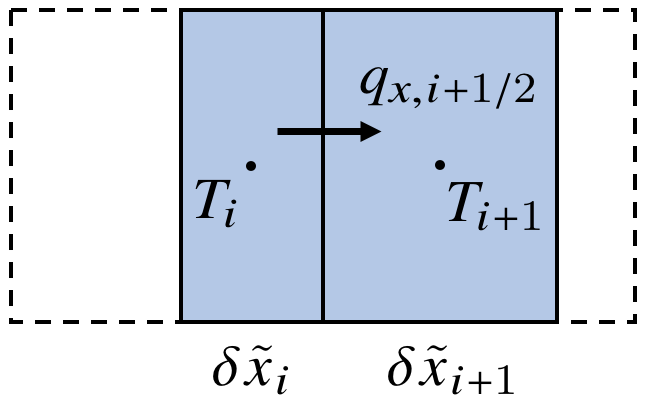
\includegraphics[height=1.25in]{FIGURES/flux_deform}
\caption{Diagram of intercell heat flux with a shrinking material.}
\label{fig:flux_deform}
\end{figure}

\noindent Calculation of the cell volumes, $\delta \tilde{x}$, etc., for pyrolysis with material deformation is discussed below.

\subsubsection*{Boundary Conditions}
\label{sec:boundary_conditions}

For two-way coupling between the gas and solid phase the boundary condition is continuity of heat flux and temperature.  On the gas phase side, the heat fluxes are due to convection and radiation, and on the solid phase side the heat flux is due to conduction.  The surface temperature links all these fluxes at an instant in time.  Let $T_{\mathrm{w}}$ denote the interface temperature between the gas and solid, the face temperature of the ``wall cell''.  The flux continuity boundary condition implies
\begin{equation}
\label{eq:fluxcontinuity}
\dot{q}_{{\mathrm{r}}, in}'' - \dot{q}_{{\mathrm{r}}, out}'' + \dot{q}_{\mathrm{c}}'' = -k_{\mathrm{s}} \left. \frac{\partial T_{\mathrm{s}}}{\partial n} \right|_{\mathrm{w}}
\end{equation}
To obtain the surface temperature, we take $\dot{q}_{{\mathrm{r}}, in}''$ from the radiation solver, linearize $\dot{q}_{{\mathrm{r}}, out}''$, and use Newton's law of cooling for $\dot{q}_{\mathrm{c}}''$. The flux condition may then be discretized as
\begin{equation}
\label{eq:discflux}
( \dot{q}_{{\mathrm{r}}, in}'' )^n + 3 \varepsilon^n \sigma \, (T_{\mathrm{w}}^n)^4 - 4 \varepsilon^n \sigma \, (T_{\mathrm{w}}^n)^3 \, T_{\mathrm{w}}^{n+1} + h^n (T_{\mathrm{g}}^n - T_{\mathrm{w}}^{n+1}) = -2 \, k_{\mathrm{s}}^n \, \frac{T_{\mathrm{s}}^n - T_{\mathrm{w}}^{n+1}}{\delta}
\end{equation}
where $T_{\mathrm{g}}$ is the gas temperature in the first off-wall grid cell and $n$ indicates the time level in the simulation.  Our result for the updated boundary temperature is
\begin{equation}
\label{eq:tmpwall}
T_{\mathrm{w}}^{n+1} = \frac{ ( \dot{q}_{{\mathrm{r}}, in}'' )^n + 3 \varepsilon^n \sigma \, (T_{\mathrm{w}}^n)^4 + h^n \, T_{\mathrm{g}}^n + 2 \, k_{\mathrm{s}}^n \, T_{\mathrm{s}}^n/\delta }{ 4 \varepsilon^n \sigma \, (T_{\mathrm{w}}^n)^3 + h^n + 2 \, k_{\mathrm{s}}^n / \delta}
\end{equation}

\subsubsection*{Surface Heat Flux Internal Wall Model}

In Eqs.~(\ref{eq:discflux}) and (\ref{eq:tmpwall}), the conductive heat flux into the wall is presumed to be resolved by a length scale, $\delta$.  In the 3D heat transfer model this length scale is \emph{not} taken to be the 3D cell spacing normal to the wall---the required 3D grid resolution would make the model intractable.  Instead, an internal wall model is employed.  To be consistent with the resolution of the 1D heat conduction model, the thermal penetration depth is taken to be
\begin{equation}
\label{eq:pendepth}
\delta = \sqrt{\frac{ \tau \; k_{\mathrm{s}}}{\rho_{\mathrm{s}} c_{\mathrm{s}}}}
\end{equation}
where $\tau$ is a somewhat arbitrary time scale set to unity.

% An alternate model for the thermal penetration depth that does not rely on an arbitrary time scale is
% \begin{equation}
% \label{eq:pendepth2}
% \delta = \left( \frac{\rho_{\mathrm{s}} \alpha_{\mathrm{s}}^3}{\dot{q}_w''} \right)^{1/3}
% \end{equation}
% where $\alpha_{\mathrm{s}} = k_{\mathrm{s}}/( \rho_{\mathrm{s}} c_{\mathrm{s}} )$.  Equation (\ref{eq:pendepth2}) is iterative since $\dot{q}_w''$ depends on $\delta$ (but convergence is very fast).  This length scale tends to be smaller than the depth given by Eq.~(\ref{eq:pendepth}).  The appropriate choice of length scale may be problem dependent.  Determining robust guidelines for grid independence of solid phase calculations is still an open area of research.  Presently, Eq.~(\ref{eq:pendepth2}) must be implemented at the source code level (there is no user hook).

\subsubsection*{Internal Radiation}
\label{sec:radiation}

The \emph{absorption coefficient} of the solid is denoted $\kappa_{\mathrm{s}}$.  If $\delta \times \kappa_{\mathrm{s}} \gg 1$, the material may be considered ``optically thick'' \cite{Modest:2003}.  This applies to many problems in pyrolysis.  The optically thick approximation implies a ``radiative conductivity'',
\begin{equation}
\label{eq:krad}
k_{\mathrm{r}} = \frac{16 n_{\mathrm{s}}^2 \sigma T_{\mathrm{s}}^3}{3 \kappa_{\mathrm{s}}} \,\mbox{,}
\end{equation}
which may simply be added to the material conductivity in the solver. Note that increasing the solid conductivity reduces the surface temperature, per Eq.~(\ref{eq:fluxcontinuity}), consistent with the notion that the radiation is not absorbed at the surface. Here, $n_{\mathrm{s}}$ is the material refractive index and $\sigma$ is the Stefan-Boltzmann constant.


\newpage
\section{Pyrolysis Models}
\label{pyrosection}

This section describes how solid phase reactions and the chemical source term in the solid phase heat conduction equation, $\dot{q}_{\rm s,c}'''$ (see Eq.~(\ref{eq:solid_energy_source_term})),  are modeled. This is commonly referred to as the ``pyrolysis model'', but it actually can represent any number of reactive processes, including evaporation, charring, and internal heating.


\subsection{Specified Heat Release Rate}

Often the intent of a fire simulation is merely to predict the transport of smoke and heat from a {\em specified} fire. In other words, the heat release rate is a specified input, not something the model predicts. In these instances, the desired heat release rate is translated into a mass flux for fuel at a given solid surface, which can be thought of as the surface of a burner:
\be
   \dm_{\rm f}'' = \frac{ f(t) \; \dq_{\rm user}''}{\Delta H_{\si{c}}}
\ee
Usually, the user specifies a desired heat release rate per unit area, $\dq_{\rm user}''$, plus a time ramp, $f(t)$, and the gas phase heat of combustion, $\Delta H_{\si{c}}$. The mass flux of fuel from the surface to the gas, $\dm_{\rm f}''$, can then be computed. A special subset of this approach is where the user also specifies a heat of combustion, density, and thickness for the burning material. If the default simple chemistry model described in Section~\ref{sec:simplechemistry}, with its single combustion reaction, is being used and there are multiple materials burning, one or more materials might have a different heat of combustion, $\Delta H_{\si{c}{\rm ,solid}}$, than the gas-phase combustion reaction. To account for this, FDS adjusts $\dm_{\rm f}''$ so that the solid phase has the appropriate mass loss rate, $\dm_{\rm f,solid}''$.
\be
\dm_{\rm f,solid}'' = \dm_{\rm f}'' \frac{\Delta H_{\si{c}}}{\Delta H_{\si{c}{\rm ,solid}}}
\ee

\subsection{Solid Fuels}

Solids can undergo simultaneous reactions under the following assumptions:
\begin{itemize}
\setlength{\itemsep}{0.0in}
\item instantaneous release of gas species
\item local thermal equilibrium between the solid and gaseous components
\item no condensation of gaseous products
\item no porosity effects\footnote{Although porosity is not explicitly included in the model, it is possible to account for it because the volume fractions defined by Eq.~(\ref{volfrac}) need not sum to unity, in which case the thermal conductivity and absorption coefficient are effectively reduced.}
\end{itemize}
Each material component may undergo several competing reactions, and each of these reactions may produce some other solid component (residue) and gaseous species according to specified yield coefficients.  These coefficients should sum to 1, but yields summing to less than 1 can account for products that are not explicitly included in the simulation.

The local density of material component $\alpha$ evolves in time according to the solid phase species conservation equation
\be
  \dod{ }{t} \left( \frac{\rho_{\rm s,\alpha}}{\rho_{\rm s}(0)} \right) =
    -\sum_{\beta=1}^{N_{\rm r,\alpha}} r_{\alpha \beta} + S_\alpha
  \label{solid_species_conservation}
\ee
where $N_{\rm r,\alpha}$ is the number of reactions for material $\alpha$, $r_{\alpha \beta}$ is the rate of reaction $\beta$ in units of \si{1/s},
and $\rho_{\rm s}(0)$ is the initial density of the material layer. $S_\alpha$ is the production rate of material component $\alpha$ as a result of
the reactions of the other components. The reaction rates are functions of solid and gas phase conditions and calculated as a combination of Arrhenius
and power functions:
\be
r_{\alpha \beta} =
    \underbrace{\left( \frac{\rho_{\rm s,\alpha}}{\rho_{\rm s}(0)}\right)^{n_{\rm s,\alpha\beta}}}_\textrm{Reactant dependency}
    \underbrace{A_{\alpha \beta} \; \exp \left(-\frac{E_{\alpha\beta}}{RT_{\rm s}}\right)}_\textrm{Arrhenius function}
    \underbrace{\left[X_{\rm O_2}(x)\right]^{n_{\rm O_2,\alpha\beta}}}_\textrm{Oxidation function}
    \underbrace{\max \big[0,S_{\rm thr,\alpha,\beta}(T_{\rm s}-T_{\rm thr,\alpha \beta}) \big]^{n_{\rm t,\alpha\beta}}}_\textrm{Power function}
   \label{Arrhenius}
\ee
The first term describes the dependence of the reaction rate on the concentration of the reactant itself, with $n_{\rm s,\alpha\beta}$ being the partial
reaction order. The second term is the Arrhenius function which is commonly used to describe the reaction kinetics, i.e. the dependence of the reaction
rate on the material temperature. The chapter on pyrolysis in the FDS Verification Guide describes methods for determining the kinetic parameters
$A_{\alpha \beta}$ and $E_{\alpha\beta}$ using bench-scale measurement techniques.

The third term can be used to describe the dependence on the
local oxygen concentration $X_{\rm O_2}(x)$ and the heterogeneous reaction order, $n_{\rm O_2,\alpha\beta}$.
The oxygen concentration profile within practical materials depends on the competition between diffusion and reactive consumption.
As FDS does not solve for the transport of gaseous species within condensed phase materials, a simple exponential profile is assumed and the
user is expected to specify the characteristic depth at which oxygen would be present.
The local oxygen volume fraction at depth $x$ is calculated from the gas phase (first grid cell) oxygen volume fraction $X_{\rm O_2,g}$ as
\be
X_{\rm O_2}(x) = X_{\rm O_2,g}\exp(-x/L_{\rm g,\alpha\beta})
\ee
where $L_{\rm g,\alpha\beta}$ is the characteristic depth of oxygen diffusion. Specifying $L_{\rm g,\alpha\beta}=0$ means that the reaction takes place
only at the surface of the material.

The fourth term is the power function where $T_{\rm thr,\alpha \beta}$ is a threshold temperature that can be used to dictate that the reaction must not occur below ($S_{\rm thr,\alpha,\beta}=+1$)  or above ($S_{\rm thr,\alpha,\beta}=-1$) a user-specified temperature. By default, the fourth term is deactivated ($S_{\rm thr,\alpha,\beta}=+1, T_{\rm thr,\alpha\beta}=0$ K).

Note that the solid species conservation equation~\ref{solid_species_conservation} and the reaction rate equation~\ref{Arrhenius} are inconsistent with the common practice of chemical kinetics convention, where the unit of the reaction rate is usually \si{kg/(m^3.s)} or \si{mol/(m^3.s)}. The current form can be obtained by dividing a more conventional reaction rate equation by $\rho_{\rm s}(0)$. This form is very close to the form used in \cite{Gpyro:FSJ} with the exception that initial layer density $\rho_{\rm s}(0)$ is used for scaling instead of the instantaneous value.

The production term $S_\alpha$ is the sum over all the reactions where the solid residue is material $\alpha$
\be
S_\alpha = \sum_{\alpha'=1}^{N_{\rm m}} \sum_{\beta=1}^{N_{\rm r,\alpha'}}
           \nu_{\alpha,\alpha' \beta} \; r_{\alpha' \beta}
       \quad \quad
           \hbox{(where Residue$_{\alpha' \beta}$ = Material$_\alpha$) }
\ee
where $\nu_{\alpha,\alpha' \beta}$ is the yield of component $\alpha$ from reaction $\beta$ of component $\alpha'$. The volumetric production rate of each gas species, $\gamma$, is
\be
\label{eq:pyrolyzate}
\dot{m}_{\gamma}''' = \rho_{\rm s}(0)\; \sum_{\alpha=1}^{N_{\rm m}} \sum_{\beta=1}^{N_{\rm r,\alpha}}
    \nu_{\rm \gamma,\alpha \beta} \; r_{\alpha \beta}
\ee
It is assumed that the gases are transported instantaneously to the surface, where the
mass fluxes are given by\footnote{In cylindrical and spherical coordinates, the mass fluxes are
\be
   \dm_\gamma'' =\frac{1}{R_{\rm out}}   \int_{R_{\rm in}}^{R_{\rm out}} \dm_\gamma'''(x) \,r \d r \;\; ; \;\;
   \dm_\gamma'' =\frac{1}{R_{\rm out}^2} \int_{R_{\rm in}}^{R_{\rm out}} \dm_\gamma'''(x) \,r^2 \d r \;\;
\ee}
\be
\label{eq:1dmassflux_solid}
\dm_\gamma'' = \int_0^L \dm_\gamma'''(x) \,\d x
\ee
where $L$ is the thickness of the solid. The chemical source term in the heat conduction equation is
\be
\label{eq:qchem_solid}
\dot{q}_{\rm s,c}'''(x) = -\rho_{\rm s}(0)\; \sum_{\alpha=1}^{N_{\rm m}} \sum_{\beta=1}^{N_{\rm r,\alpha}}  r_{\alpha \beta}(x) H_{\rm r,\alpha \beta}
\ee
where $H_{\rm r,\alpha \beta}$ is the heat of reaction.

\subsection{Phase Change Reactions}

To describe freezing or melting of liquids, the two phases are separated by a sharp interface at the constant phase-change temperature, $T_{\rm f}$. The location of the phase boundary $x_{\rm f}$ is governed by the equation
\be
k_{\rm s,1} \dod{T_{\rm s,1}}{x}-k_{\rm s,2}\dod{T_{\rm s,2}}{x} = \rho_{\rm s} H_{\rm r,\alpha\beta} \dod{x_{\rm f}}{t}
\ee
where 1 and 2 refer to the materials on the two sides of the boundary. In the context of the fixed-grid finite-difference method, it is more convenient
to allow a small deviation from $T_{\rm f}$ and solve for the amount of mass reacting during the time step, $\Delta t$,
from the energy required to convert the mass from one phase to the other
\be
\dot{m}''' \Delta t = \frac{\rho_{\rm s} c_{\rm s}(T_{\rm s}-T_{\rm f})}{H_{\rm r,\alpha\beta}}
\ee
This reaction can be implemented by setting $T_{\rm thr,\alpha\beta} = T_{\rm f}$ and $A_{\alpha\beta} = c_{\rm s}$ and turning on a specific
{\em phase-change reaction} mode. The reaction rate given by Eq.~\ref{Arrhenius} is then divided by the factor $H_{\rm r,\alpha\beta} \Delta t$.

\subsection{Liquid Fuels}

Consider a liquid consisting of one or more components. The evaporation rate of each evaporating liquid component, $\alpha$, is governed by the following relation:
\be
\dot{m}_\alpha'' = h_{\rm m} \, \rho_{\rm film} \, \ln \left( 1+B \right) \left( Y_{\alpha,{\rm sv}}+\frac{Y_{\alpha,{\rm sv}}-Y_{\alpha,{\rm g}}}{B} \right) \quad ; \quad B=\frac{\sum_{\alpha'} (Y_{\alpha',{\rm sv}}-Y_{\alpha',{\rm g}})}{1-\sum_{\alpha'} Y_{\alpha',{\rm sv}}}  \label{mdot_alpha}
\ee
$h_{\rm m}$ is the mass transfer coefficient, $\rho_{\rm film}$ is the density within a thin surface layer, $B$ is the Spalding mass transfer number, $Y_{\alpha,{\rm sv}}$ is the ``surface vapor'' mass fraction of component $\alpha$ at the liquid surface, and $Y_{\alpha,{\rm g}}$ is the mass fraction of component $\alpha$ in the center of the grid cell adjacent to the liquid surface. The composition of the surface layer is obtained using Raoult's law with the Clausius-Clapeyron equation for the equilibrium vapor pressure.  The volume fraction of component $\alpha$ at the surface is:
\be
   X_{\alpha,{\rm sv}} = X_{\alpha,\ell} \, \exp \left[ -\frac{ h_{\rm v,\alpha} W_{\alpha}}\R \left(\frac{1}{T_{\rm s}}-\frac{1}{T_{\rm b,\alpha}} \right) \right]  \quad ; \quad
   Y_{\alpha,{\rm sv}} = \frac{X_{\rm \alpha,sv} W_{\alpha} }{\sum_{\alpha'} X_{\rm \alpha',sv} W_{\alpha'} + (1-\sum_{\alpha'} X_{\rm \alpha',sv}) W_{\rm air} }
   \label{CC_liquid}
\ee
Here $X_{\alpha,\ell}$ is the volume fraction of component $\alpha$ in the liquid, $h_{\rm v,\alpha}$ is its heat of vaporization, $W_\alpha$ is its molecular weight, $T_{\rm b,\alpha}$ is its boiling temperature, and $T_{\rm s}$ is the surface temperature.  The mass transfer coefficient is given by
\be
h_{\rm m}= \frac{\SH \, D_{\rm film}}{L} \quad ; \quad \SH=0.037~\SC^{\frac{1}{3}} \RE^{\frac{4}{5}} \quad ; \quad {\rm Sc}=\frac{ \mu_{\rm film} }{ \rho_{\rm film} \, D_{\rm film}} \quad ; \quad \RE= \frac{\rho_{\rm film}~||\bu||~L}{\mu_{\rm film}}
\ee
Sh is the Sherwood number and $D$ is the mole-weighted gas phase diffusivity:
\be
   D_{\rm film} = \frac{ \sum_\alpha X_{\alpha,{\rm sv}} D_\alpha }{\sum_\alpha X_{\alpha,{\rm sv}} }
\ee
where $D_\alpha$ is the diffusivity of species $\alpha$ into air evaluated at the film temperature. The Reynolds number is based on the gas velocity in the gas cell adjacent to the surface, $||\bu||$, the length scale, $L$, and the density and viscosity of the surface film. The length scale, $L$, is 1~m for a liquid pool unless specified otherwise. The film density is
\be
   \rho_{\rm film} = \frac{ p_0 }{ \R \, T_{\rm film} \, \left( \sum_\alpha Y_{\alpha,{\rm sv}}/W_\alpha + (1-\sum_\alpha Y_{\alpha,{\rm sv}})/W_{\rm air} \right) }
\ee
It is assumed that the composition of the film layer consists of evaporated liquids and air.

In practice, a liquid fuel may have multiple components, like gasoline or kerosene, but for the sake of reducing CPU time, all liquid components can be assumed to evaporate to form a common lumped gas species whose mass fraction is denoted $Z_{\rm g}$. In this case, the effective mass fraction of gas species $\alpha$ is assumed to be proportional to its value at the liquid surface:
\be
   Y_{\rm \alpha,g} = Z_{\rm g} \frac{Y_{\rm \alpha,sv}}{\sum_{\alpha'} Y_{\alpha',{\rm sv}}}
\ee
The assumption of an assumed lumped gas species is not mandatory---one can evaporate each liquid component to form a unique gas species.

For simplicity, the liquid fuel itself is treated like a thermally-thick solid for the purpose of computing the heat conduction. There is no computation of the convection of the liquid within the pool. Obviously, this assumption has consequences. One of which is related to the fact that the evaporation rate expression ({\ref{mdot_alpha}) is applied only to the surface liquid layer. However, it is possible that an interior liquid layer may possess a temperature, $T_\ell$, in excess of the boiling temperature of an individual liquid component, $T_{\rm b,\alpha}$. If this is the case, an additional amount of component $\alpha$ is boiled off from the surface so as to drive the liquid temperature back towards the boiling point of component $\alpha$. This addition to the surface mass flux takes the form:
\be
   \dot{m}_\alpha'' = \frac{ \rho_{\ell,\alpha} \left( h(T_{\ell})-h(T_{\rm b,\alpha}) \right) \delta}{h_{\rm v,\alpha} \dt} \quad ; \quad  h(T) = \int_0^T  c_s(T') \d T'
\ee
where $\rho_{\ell,\alpha}$ is the mass per unit volume of liquid component $\alpha$, $h(T)$ is the enthalpy of the liquid, $\delta$ is the layer thickness, $h_{\rm v,\alpha}$ is the heat of vaporization of component $\alpha$, and $\dt$ is the time step.





\subsection{Shrinking and Swelling Materials}
\label{sec:shrink_swell}

The layer thickness is updated according to the ratio of the instantaneous material density and the density of the material in its pure form. In case of several material components, the amount of swelling and shrinking is determined by the maximum and sum of these ratios, respectively. In each time step, the size of each condensed phase cell is multiplied by the following factor:
\be
\delta =
   \begin{cases}
   \max_{\alpha}\left(\frac{\rho_{\rm s,\alpha}}{\rho_\alpha}\right) & \text{if }\max_{\alpha}\left(\frac{\rho_{\rm s,\alpha}}{\rho_\alpha}\right) \geq 1 \\
   \sum_{\alpha}\left(\frac{\rho_{\rm s,\alpha}}{\rho_\alpha}\right) & \text{if }\max_{\alpha}\left(\frac{\rho_{\rm s,\alpha}}{\rho_\alpha}\right) < 1
   \end{cases}
\ee
Correspondingly, the densities are divided by the factor $\delta$ to conserve mass.

\subsection{Solid Pyrolysis 3D (Beta)}

To begin our discussion of pyrolysis it is useful to start with definitions of the material mass density and volume.  We consider a solid composed of a mixture of material components $\alpha$.  The \emph{material density} (a property of the material) is
\begin{equation}
\label{eq:matden}
\rho_\alpha \equiv \frac{m_\alpha}{V_\alpha}
\end{equation}
The \emph{bulk density} is
\begin{equation}
\label{eq:bulkden}
\rho_{\mathrm{s},\alpha} \equiv \frac{m_\alpha}{V_{\mathrm{s}}}
\end{equation}
And the \emph{total solid density} is
\begin{equation}
\label{eq:totalsolidden}
\rho_{\mathrm{s}} \equiv \sum_\alpha \rho_{\mathrm{s},\alpha}
\end{equation}

The reaction kinetics and heat source terms are the same in 1D and 3D.  The bulk density of material component $\alpha$ evolves by Eq.~(\ref{solid_species_conservation}) and the chemical heat source term is given by Eq.~(\ref{eq:qchem_solid}).

\subsubsection*{Local Material Deformation}
\label{sec:locmatdef}

A discussion about how the 1D model handles shrinking and swelling materials can be found in Sec.~\ref{sec:shrink_swell}.  In this section, we deal with the same issue in 3D.  One of the key differences in the 1D and 3D models is that the concept of ``thickness'' in the 1D model is not dependent at all on the 3D computational mesh.  In the 1D solver, the material shrinks from the bottom up, with the face of the solid stationary (until the cell potentially burns away).

Conversely, in 3D the solid mass is tied to the Eulerian grid cell.  The grid cell itself cannot disappear.  Instead we track the solid volume relative to the local cell volume.  This volume ratio may be computed from the material densities as follows:
\begin{equation}
\label{eq:volratio}
\phi_{\mathrm{s}} \equiv \frac{V_{\mathrm{s}}}{V_{\mathrm{cell}}} = \frac{\sum_\alpha V_\alpha}{V_{\mathrm{cell}}} = \sum_\alpha \frac{m_\alpha/\rho_\alpha}{m_\alpha/\rho_{\mathrm{s},\alpha}} = \sum_\alpha \frac{\rho_{\mathrm{s},\alpha}}{\rho_\alpha}
\end{equation}

We presently consider two simple models for material deformation: isotropic and unidirectional.  The method is based on the definition $V_{\mathrm{s}}= \phi_{\mathrm{s}} V_{\mathrm{cell}}$, which is equivalent to $\prod_i \delta \tilde{x}_i = \phi_{\mathrm{s}} \prod_i \delta x_i$. For a 2D case, if the material deforms equally in both directions (isotropic) then the spacing used to compute heat fluxes is computed from
\begin{align}
\label{eq:dxdefiso}
\delta \tilde{x} &= \phi_{\mathrm{s}}^{1/2} \delta x \nonumber\\
\delta \tilde{y} &= \phi_{\mathrm{s}}^{1/2} \delta y
\end{align}

If, on the other hand, we have a preferred direction for mass loss (such as in a cone calorimeter test), then the deformation is considered unidirectional.  The flux spacing is computed as (deformation in $x$)
\begin{align}
\label{eq:dxdefuni}
\delta \tilde{x} &= \phi_{\mathrm{s}} \delta x \nonumber\\
\delta \tilde{y} &= \delta y
\end{align}

\subsection{Mass Transport}
\label{sec:mass_transport}

The movement of pyrolysis gas through the material to the solid surface is complicated to model in detail.  In many practical codes, mass transfer resistance is simply ignored.  Thus, any gas generated via pyrolysis is imagined to instantaneously appear at the solid surface as a mass flux boundary condition to the gas phase.  The 3D model allows both instantaneous transport and diffusive transport, which we discuss below.

\subsubsection*{Gas Generation}
\label{eq:gas_generation}

Similar to Eq.~(\ref{eq:pyrolyzate}), in 3D the mass generation rate per unit volume of pyrolysis gas component $\gamma$ in cell $i,j,k$ is given by
\begin{equation}
\label{eq:massprod}
\dot{m}_{\gamma,i,j,k}''' = \rho_{\mathrm{s}}(0)_{i,j,k} \sum_{\alpha=1}^{N_{\mathrm{m}}} \sum_{\beta=1}^{N_{\mathrm{r},\alpha}} \nu_{\gamma,\alpha\beta} r_{\alpha\beta,i,j,k}
\end{equation}

\subsubsection*{Instantaneous Transport}
\label{sec:instantaneous_transport}

Similar to the 1D model, instantaneous transport is the default mode of operation in the 3D model.  However, implementation is not as straight-forward in 3D since Eulerian cells more than one cell below the surface are not usually tied to a ``wall cell''.  In 3D, unless the user specifies otherwise, mass is ejected via the nearest wall cell and the deformation model is taken to be isotropic.  Alternatively, the user may specify the direction for mass ejection and the deformation model becomes unidirectional.

For instantaneous transport, the mass flux at the solid surface for a given wall cell is the summation of the mass production in the column of solid cells tied to the wall cell.  For a column of cells in the $z$ direction tied to wall cell $w$, we have
\begin{equation}
\label{eq:mdotint}
\dot{m}_{\gamma,w}'' = \sum_{k \in w} \dot{m}_{\gamma,i,j,k}''' \,\delta z_k
\end{equation}
This is the 3D discrete analog of Eq.~(\ref{eq:1dmassflux_solid}).

\subsubsection*{Diffusive Transport}
\label{sec:diffusive_transport}

A less arbitrary way to assign the pyrolysis gas to a wall cell is to simply solve a transport equation.  While the physics is not so simple in reality, an isotropic diffusion model of transport has several advantages:  It is easy to implement.  It avoids any ad hoc assumptions applied in the instantaneous model.  It handles smoldering combustion and char oxidation naturally.  And finally, while the physics are not perfect, they are usually qualitatively correct and the implementation lends itself to improvement.

The diffusive transport equation for gas component $\gamma$ is given by
\begin{equation}
\label{eq:diff}
\frac{\partial \rho_\gamma}{\partial t} = - \Div\mathbf{J}_\gamma + \dot{m}_{\gamma}'''
\end{equation}
where the diffusive flux is modeled with Fick's law,
\begin{equation}
\label{eq:fick}
\mathbf{J}_\gamma = - D_{\gamma} \tilde{\nabla} \rho_\gamma
\end{equation}
Note that the gradient operator is written in terms of a deformed space coordinate, in the same manner as the heat flux.  In the current implementation, the diffusivity is isotropic.  The default is the gas phase molecular value for component $\gamma$.  However, the user may adjust this value if needed.

\subsubsection*{Transport Boundary Conditions}
\label{sec:transport_bcs}

Consider the flux between solid cell $i$ and gas phase cell $i+1$.  The surface is denoted by F for ``face value''. The mass flux at the solid surface is taken from
\begin{equation}
\label{eq:massflux_boundary}
J_{\gamma,\mathrm{F}} = - D_{\gamma,\mathrm{F}} \frac{\rho_{\gamma,\mathrm{F}} - \rho_{\gamma,i}}{\frac{1}{2}\delta \tilde{x}_i}
\end{equation}
where
\begin{equation}
\label{eq:rhoF}
\rho_{\gamma,\mathrm{F}} =
\left\{\begin{array}{ll}
0                          & \mbox{if $\gamma$ is fuel} \\
\rho Y_{\gamma,\mathrm{F}} & \mbox{if $\gamma$ is oxidizer} \\
\rho_{\gamma,i}            & \mbox{if boundary is impermeable, $J_{\gamma,\mathrm{F}}=0$}
\end{array}\right.
\end{equation}

The boundary conditions in Eq.~(\ref{eq:rhoF}) provide qualitatively correct behavior for the pyrolysis gases (transport \emph{out} of the solid) while allowing diffusion of oxidizer into the solid.  Using $\rho Y_{\gamma,\mathrm{F}}$ for the fuel can lead to erratic behavior caused by diffusion of fuel back into the solid, which is not physical.  This ad hoc treatment of the boundary is a limitation of the diffusion model, but we note that the scheme is no worse than the instantaneous transport out of the solid used in most 1D models.

It should be noted that $\rho Y_{\gamma,\mathrm{F}}$ is currently taken from the gas phase solver at the current time level.  The mass flux is therefore time lagged between the gas phase and solid phase solvers, unlike the surface temperature from Eq.~(\ref{eq:tmpwall}).  This is a potential source of error that will be addressed in future development.



% !TEX root = FDS_Technical_Reference_Guide.tex

\typeout{new file: Particle_Chapter.tex}

\chapter{Lagrangian Particles}
\label{chapter:lagrangian_particles}

Lagrangian particles are used to represent a wide variety of objects that cannot be resolved on
the numerical grid. Liquid droplets are the most common example. This chapter outlines the treatment of the transport, size
distribution, and mass, momentum and energy transfer to and from Lagrangian particles.  The formulation presented here closely follows the dispersed discrete-element formulation presented in \cite{Crowe:1}.

\section{Particle Transport in the Gas Phase}

In the gas phase momentum equation, Eq.~(\ref{momentum}), the force term $\bof_{\rm b}$ represents the momentum transferred from particles to the gas. It is obtained by summing the force transferred from each particle in a grid cell and dividing by the cell volume, $V$:
\be
    {\bof_{\rm b}} = \frac{1}{V} \sum  \left[ \frac{\rho}{2} \, C_{\rm d} \, A_{\rm p,c} \, (\bu_{\rm p}-\bu) |\bu_{\rm p}-\bu| - \frac{\d m_{\rm p}}{\d t} \, (\bu_{\rm p}-\bu) \right] \label{part_force}
\ee
where $C_{\rm d}$ is the drag coefficient, $A_{\rm p,c}$ is the particle cross-sectional area, $r_{\rm p}$ is the particle radius, $\bu_{\rm p}$ is the particle velocity, $m_{\rm p}$ is the particle mass, $\bu$ is the gas velocity, and $\rho$ is the gas density. The subscript ``b'' stands for ``bulk,'' meaning that the particles in the cell represent a bulk mass dragging on the gas.

The particle acceleration is given by
\be
    \frac{\d \bu_{\rm p}}{\d t} = \bg - \ha \frac{\rho\,C_{\rm d} \, A_{\rm p,c}}{m_{\rm p}} \,
    (\bu_{\rm p}-\bu) |\bu_{\rm p}-\bu|
    \label{part_accel}
\ee
The particle position, $\bx_{\rm p}$, is determined from the equation
\be
    \frac{\d \bx_{\rm p}}{\d t} = \bu_{\rm p}
\ee
The exact solution procedure of the above model is presented in Appendix~\ref{particle_momentum_transfer}. The drag coefficient (default based on a sphere) is a function of the local Reynolds number that is based on the particle diameter, $D$ ($2 r_{\rm p}$)
\begin{align}
 C_{\rm d} &= \left\{ \begin{array}{ll}
     24/\RE_D                                          & \RE_D < 1    \\[0.1in]
     24\left(0.85+0.15 \, \RE_D^{0.687} \right)/\RE_D  & 1 < \RE_D < 1000 \label{sphere_drag}\\[0.1in]
     0.44                                              & 1000 < \RE_D
     \end{array} \right.  \\[0.2in]
\RE_D &= \frac{\rho \, |\bu_{\rm p}-\bu| \, 2 r_{\rm p}}{\mu(T)} \end{align}
where $\mu(T)$ is the dynamic viscosity of air at temperature $T$~\cite{Crowe:1}\footnote{Note that the 0.85 in the second line of Eq.~(\ref{sphere_drag}) has been inserted to ensure continuity of the functional relationship at $\RE_D=1$.}. For cylindrical particles, the following correlation was derived from data presented by Schlichting~\cite{Schlichting:1}:
\begin{align}
 C_{\rm d} &= \left\{ \begin{array}{ll}
     10/\RE_D^{0.8}                                & \RE_D < 1    \\[0.1in]
     10\left(0.6+0.4 \, \RE_D^{0.8} \right)/\RE_D  & 1 < \RE_D < 1000 \\[0.1in]
     1                                             & 1000 < \RE_D
     \end{array} \right.
\end{align}
Additional corrections are made to account for drag reduction due to the wake effect~\cite{Ramirez:1} and deformation of the droplet~\cite{Loth:1}.


\subsection{Using Lagrangian Particles to Represent Vegetation}

For some applications, it is convenient to use Lagrangian particles to represent stationary vegetation, like grasses or leaves, or airborne vegetation, like burning brands. Typically, these different types of vegetation are grouped into different classes of fuel ``elements'', each of which is represented by a single representative particle in each grid cell. Each representative particle contributes to the bulk force term:
\be
    {\bof_{\rm b}} = \sum_{\rm e} {\bof_{\rm b,e}} \quad ; \quad {\bof_{\rm b,e}} = \frac{\rho}{2} \, C_{\rm d} \, C_{\rm s,e} \,  \beta_{\rm e} \, \sigma_{\rm e} \, (\bu_{\rm p,e}-\bu) |\bu_{\rm p,e}-\bu| + \dot{m}_{\rm p,e}''' \, (\bu_{\rm p,e}-\bu)   \label{part_force_veg}
\ee
The terms with subscript ``e'' refer to a particular class of fuel \underline{e}lements and are determined geometrically or empirically.  The shape factor, $C_{\rm s,e}$, is the ratio of the particle's projected cross sectional area, $A_{\rm p,c}$, to its surface area, $A_{\rm p,s}$. A perfect sphere has a shape factor of $\pi r^2/4 \pi r^2=1/4$, but for actual vegetation, the shape factor is assigned an empirical value that accounts for both shape and orientation. Pine needles, for example, project a different cross sectional area depending on their orientation. The drag coefficient, $C_{\rm d}$, is empirically derived and takes into account both the geometry and shadowing effects of closely packed objects. It is typically expressed as a constant rather than a function of the Reynolds number.  $\beta_{\rm e}$ is the volume fraction; that is, the ratio of the volume occupied by solid mass to the overall volume of the vegetation, sometimes referred to as the {\em packing ratio}. $\sigma_{\rm e}$ is the surface to volume ratio of a single particle. $\dot{m}_{\rm p,e}'''$ is the mass generation rate per unit volume of that particular vegetation element.

A convenient way to describe the geometric properties of vegetation is by specifying the surface to volume ratio, $\sigma_{\rm e}$, the volume (packing) ratio, $\beta_{\rm e}$, and an assumed shape, like a sphere or cylinder. The volume fraction is sometimes expressed as a mass per unit volume, or {\em bulk density}, $m'''=\rho_{\rm e} \, \beta_{\rm e}$, where $\rho_{\rm e}$ is the density of the solid. With this information, and the following relations:
\be
   C_{\rm s,e} = \frac{A_{\rm p,c}}{A_{\rm p,s}} \quad ; \quad  \beta_{\rm e}=\frac{n_{\rm p,e} \, V_{\rm p}}{V} = \frac{m'''}{\rho_{\rm e}} \quad ; \quad \sigma_{\rm e}=\frac{A_{\rm p,s}}{V_{\rm p}}
\ee
we can convert the drag force expression in Eq.~(\ref{part_force_veg}) to its equivalent in Eq.~(\ref{part_force}) where the single particle element is represented as $n_{\rm p,e}$ spheres or cylinders occupying a grid cell volume, $V$. In the model, it is sufficient to have only one weighted particle per grid cell per fuel element to represent all of the actual particles of that vegetation class.

One further simplification of Eq.~(\ref{part_force_veg}) is made by lumping terms into a single {\em frontal area density}
\be
   \kappa_{\rm e} = C_{\rm s,e} \,  \beta_{\rm e} \, \sigma_{\rm e} = \frac{ n_{\rm p,e} \, A_{\rm p,c}}{V} \label{kappa_eq}
\ee
$\kappa_{\rm e}$ can also be thought of as an {\em absorption coefficient} for the purpose of computing thermal radiation absorption. In practice, $\kappa_{\rm e}$ is not determined from Eq.~(\ref{kappa_eq}). Rather, it is obtained by measuring the relative amount of sunlight that penetrates a slab of vegetation of thickness, $L$:
\be
   W = {\rm e}^{-\kappa_{\rm e} L}
\ee
Here, $W$ is the relative area of ``white'' of the shadowgraph formed by sunlight passing through the vegetation. It can also be thought of as the fraction of blue sky one sees when looking through a tree canopy of thickness $L$. It is often referred to as the {\em frontal area index} or {\em frontal area fraction}, not to be confused with the {\em frontal area density}, $\kappa_{\rm e}$.

\subsection{Drag Reduction}
\label{sec:threeway}

Typically, Lagrangian particle models only consider two-way coupling between the gas and particles. This means that each particle interacts with the carrier fluid individually. Momentum lost from a particle is added to the fluid and vice versa. If the spray is dense enough, however, the individual particles influence each other through aerodynamic interactions. These effects cannot be captured by the current Eulerian-Lagrangian model for two reasons. First, the Lagrangian particles occupy no volume in the Eulerian space. Second, the separation lengths would be of sub-grid scale in most practical simulations. The aerodynamic interactions start to have an effect when the average particle spacing is less than 10 diameters~\cite{Prahl:1,Prahl:2}. This corresponds to a particle volume fraction, $\alpha$, of approximately 0.01. Volume fractions as high as this can sometimes be achieved inside water mist sprays. If the spray is even more dense, particle-particle collisions or four-way coupling would need to be considered.

In a configuration where two particles with the same diameter are directly in line, the reduction of the drag force on the second particle can be modeled by the following~\cite{Ramirez:1}:
\be
  C_{\rm d} = C_{\rm d,0} \, \frac{F}{F_0}, \label{eq:dragred}
\ee
where $C_{\rm d,0}$ is the single particle drag coefficient and $F / F_0$ is the hydrodynamic force ratio of the trailing particle to an isolated particle:
\be
  \frac{F}{F_0} = W \left[ 1 + \frac{\RE}{16} \frac{1}{\left( L / D - 1
  / 2 \right)^2} \exp \left( - \frac{\RE}{16} \frac{1}{\left( L / D - 1
  / 2 \right)^{}} \right) \right]. \label{eq:dragredfact}
\ee
where $\RE$ is the single particle Reynolds number, $L$ is the distance between the particles, and $W$ is the non-dimensional, non-disturbed wake velocity at the center of the trailing particle
\be
  W = 1 - \frac{C_{\rm d,0}}{2} \left[ 1 - \exp \left( - \frac{\RE}{16}
  \frac{1}{\left( L / D - 1 / 2 \right)} \right) \right]. \label{eq:Wake-Vel}
\ee
This model assumes that the spheres are traveling directly in-line with each other. As such, this provides an upper bound for the strength of the aerodynamic interactions between two particles of the same size. The average separation distance $L/D$ between particle centers is calculated from the local particle volume fraction, $\alpha$, as follows:
\be
  L/D = \left(\pi/6\alpha \right)^{\frac{1}{3}}.
\ee
This simple approximation assumes that particles are uniformly distributed in each computational cell~\cite{Bhattacharyya2008}.

In reality, the spray is not monodisperse and the separation distance between the interacting particles varies. In the simulation, the drag reduction factor in Eq.~\ref{eq:dragred} is only used when the local droplet volume fraction exceeds \num{1e-5}. The drag reduction model is turned on by default.

As $L/D$ approaches zero, the drag coefficient approaches
\be
  C_{\rm d} = C_{\rm d,0} \left(1 - \frac{C_{\rm d,0}}{2}\right),
\ee
which is 78\% of that for an isolated spherical particle.

An alternative approach to drag reduction was provided by Prahl et al.~\cite{Prahl:1} who studied the interaction between two solid spheres in steady or pulsating flow by detailed numerical simulations. According to their study, the above equation underestimates the drag reduction significantly at small drop-to-drop distances. The inflow pulsations were found to reduce the effect of the drag reduction. At large distances, the two results are similar, the Ram\'{\i}rez-Mu\~{n}oz correlation showing more drag reduction. This is not surprising since the velocity profile of a fully developed axi-symmetric wake behind an axi-symmetric body is used in developing the drag reduction correction in Eqs.~\ref{eq:dragredfact} and \ref{eq:Wake-Vel}. At short distances, the wake is not fully developed and the assumption does not hold.

\section{Liquid Droplet Size Distribution}

The cumulative volume distribution for a liquid spray is represented by a combination of log-normal and Rosin-Rammler distributions~\cite{Chan:1}:
\be F_{\rm v}(D) = \left\{ \begin{array}{ll}
   \frac{1}{\sqrt{2\pi}} {\displaystyle \int_0^D} \, \frac{1}{\sigma\, D'} \,
   \exp \left( -\frac{[\ln(D'/D_{\rm v,0.5})]^2}{2\sigma^2} \right) \; \d D'            & (D \le D_{\rm v,0.5}) \\ [0.2in]
   1 - \exp \left( -0.693 \left(\frac{D}{D_{\rm v,0.5}}\right)^\gamma \right)           & (D > D_{\rm v,0.5})
   \end{array} \right.  \ee
where $D_{\rm v,0.5}$ is the median volumetric droplet diameter (i.e., half the mass is carried by droplets with diameters of $D_{\rm v,0.5}$ or less), and $\gamma$ and $\sigma$ are empirical constants equal to approximately 2.4 and 0.48, respectively.\footnote{The Rosin-Rammler and log-normal distributions are smoothly joined if $\sigma=2/(\sqrt{2\pi} \, (\ln\,2) \; \gamma)=1.15/\gamma$ .} Alternatively, the user may specify any form of size distribution using the tabulated input data.

The median droplet diameter is a function of the sprinkler orifice diameter, operating pressure, and geometry. Research at Factory Mutual has yielded a correlation for the median droplet diameter~\cite{Yu:2}
\be
   \frac{D_{\rm v,0.5}}{d} \propto \WE^{-\ot}  \label{dropcor}
\ee
where $d$ is the orifice diameter of the nozzle. The orifice Weber number, the ratio of inertial forces to surface tension forces, is given by
\be
   \WE = \frac{\rho_{\rm p} \, u_{\rm p}^2 \, d}{\sigma}  \label{Weber}
\ee
where $\rho_{\rm p}$ is the liquid density, $u_{\rm p}$ is the discharge velocity, and $\sigma$ is the liquid surface tension (\SI{72.8e-3}{N/m} at \SI{20}{\degreeCelsius} for water).
The discharge velocity can be computed from the mass flow rate, a function of the operating pressure and orifice coefficient known as the K-factor. FM reports that the constant of proportionality in Eq.~(\ref{dropcor}) appears to be independent of flow rate and operating pressure. Three different sprinklers were tested in their study with orifice diameters of \SI{16.3}{\milli m}, \SI{13.5}{\milli m}, and \SI{12.7}{\milli m}, and the constants were approximately 4.3, 2.9, and 2.3, respectively. The strike plates of the two smaller sprinklers were notched, while that of the largest sprinkler was not~\cite{Yu:2}.

In real sprinkler systems, the operating pressure is affected by the number of open nozzles. Typically, the pressure in the piping is high when the first sprinkler activates, and
decreases when more and more sprinkler heads are activated. The pipe pressure has an effect on flow rate, droplet velocity and droplet size distribution. FDS does not predict the variation of pipe pressure; it should be specified by the user. The following dependencies are used to update the droplet boundary conditions for mass flow, droplet speed, and median diameter:
\be
    \dot{m}_{\rm p} \propto p^{1/2} \quad ; \quad u_{\rm p} \propto p^{1/2} \quad ; \quad D_{\rm v,0.5}  \propto  p^{-1/3}
\ee
The droplet diameters are randomly chosen from the given size distribution. The cumulative number fraction (CNF), $F_{\rm n}$, is determined from the cumulative volume fraction, $F_{\rm v}$, as follows
\be
   F_{\rm n}(D) = \int_0^D \frac{F'_{\rm v}(D')}{D'^3} \, \d D'  \left/ \int_0^\infty \, \frac{F'_{\rm v}(D')}{D'^3}
     \, \d D' \right. \quad ; \quad F_{\rm v}' \equiv \frac{\d F_{\rm v}}{\d D}
\ee
Figure~\ref{rosin} displays the Rosin-Rammler/log-normal function and the resulting cumulative number fraction.
\begin{figure}[t]
\begin{center}
\includegraphics[width=4.5in]{SCRIPT_FIGURES/particle_size_distribution}
\caption[Liquid droplet size distribution]{Cumulative Volume Fraction and Cumulative Number
Fraction functions of the droplet size distribution from
a typical industrial-scale sprinkler. The median volumetric diameter, $D_{\rm v,0.5}$, is
1~mm, $\sigma=0.48$ and $\gamma=2.4$.}
\label{rosin}
\end{center}
\end{figure}

The selection of droplet diameters makes use of a stratified sampling technique to ensure that the droplets span the entire range of sizes, even with a relatively small number of droplets. Without the stratification, the tails of the distribution can be poorly represented. The procedure for selecting droplet sizes is as follows:
\begin{enumerate}
\item Suppose that the mass flow rate of the liquid is $\dm$, that the time interval for droplet insertion is $\dt$, and that the number of droplets inserted each time interval is $N$.
\item Divide the droplet diameter range into a number of bins of equal width.
\item Randomly choose $N$ integers, $n_i$, ranging from 1 to the total number of bins.
\item Choose $N$ uniformly distributed real numbers between 0 and 1 and calculate $N$ random droplet diameters:
\be
   D_i = F^{-1}_{\rm n} \Big[ F_{\rm n}(D_{n_i,\min}) + {\cal U}(0,1)\left(F_{\rm n}(D_{n_i,\max})-F_{\rm n}(D_{n_i,\min}) \right) \Big] \label{Ud_strat}
\ee
where ${\cal U}(0,1)$ is a uniformly distributed real number between 0 and 1 and $D_{n_i,\min}$ and $D_{n_i,\max}$ are the minimum and maximum diameters of bin $n_i$.
\item Compute weighting constants for each droplet $C_i = F_{\rm n}(D_{n_i,\max}) - F_{\rm n}(D_{n_i,\min})$.
\item Compute a global weighting constant, C, to maintain the overall mass balance:
    \be \dm \; \dt = C \, \sum_{i=1}^N \; C_i \; \frac{4}{3} \pi \rho_{\rm p}
      \left( \frac{D_i}{2} \right)^3
    \ee
    The mass and heat transferred from each droplet will be multiplied by the weighting factor $C$.
\end{enumerate}


\section{Spray Initialization}

The droplets are introduced into the simulation along a spherical surface whose diameter is a specified stand-off distance from the nozzle orifice. It is assumed that the droplets have fully atomized by this stage. The longitude of the initial droplet position, $0\le \theta < 2 \pi$, is randomly chosen from a uniform distribution. The latitude, $0 \le \phi < \pi$, is randomly selected from the following distribution:
\begin{equation}
  f(\phi) = \exp \left[ - \beta \left( \frac{\phi - \phi_{\min}}{\phi_{\max} - \phi_{\min}} \right)^2 \right]
\end{equation}
Note that $\phi=0$ is the south pole of the sphere. The spread parameter, $\beta$, is 5 by default. All the droplets are given the same initial speed in the direction of the surface normal.



\section{Heating and Evaporation of Liquid Droplets}

Liquid droplets can represent either discrete airborne spheres or elements of the thin liquid film that forms on wetted solids. These film ``droplets'' are still individually tracked as Lagrangian particles, but the heat and mass transfer coefficients are different. In the discussion to follow, the term ``droplets'' will be used to describe either form.

Over the course of a time step of the gas phase solver, the droplets in a given grid cell evaporate to form the gas species $\alpha$. The evaporation rate is a function of the liquid equilibrium vapor mass fraction, $Y_{\rm \alpha,\ell}$, the local gas phase vapor mass fraction, $Y_{\rm \alpha,g}$, the (assumed uniform) droplet temperature, $T_{\rm p}$, and the local gas temperature, $T_{\rm g}$. The subscript ``g'' refers to the average of the quantity in the cell occupied by the droplet. The subscript ``p'' refers to the liquid droplet. If the droplet is attached to a solid, $T_{\rm s}$ is the surface temperature. The mass and energy transfer between the gas and the liquid can be described by the following set of equations~\cite{Cheremisinoff:1}
\begin{align}
\frac{\d m_{\rm p}}{\d t} & = - A_{\rm p,s} \, h_{\rm m} \, \rho_{\rm f} \, (Y_{\alpha,\ell} - Y_{\rm \alpha, g}) \label{droplet_mass} \\[0.2in]
\rho_{\rm g} V \frac{\d Y_{\rm \alpha, g}}{\d t} & = -\left(1-Y_{\rm \alpha, g}\right)\frac{\d m_{\rm p}}{\d t}  \label{droplet_gas_fraction} \\[0.2in]
\frac{\d T_{\rm p}}{\d t} & = \frac{1}{m_{\rm p} \, c_{\rm p}}  \left[ \dq_{\rm r} + A_{\rm p,s} \, h_{\rm g}  \, (T_{\rm g}-T_{\rm p}) + A_{\rm p,s} \, h_{\rm w}  \, (T_{\rm w}-T_{\rm p}) + \frac{\d m_{\rm p}}{\d t} \; h_{\rm v} \right]  \label{droplet_temp}  \\[0.2in]
\frac{\d T_{\rm g}}{\d t} & = \frac{1}{m_{\rm g} \, c_{\rm g}}  \left[A_{\rm p,s} \, h_{\rm g}  \, (T_{\rm p}-T_{\rm g}) - \frac{\d m_{\rm p}}{\d t} \; (h_{\rm \alpha,p}-h_{\rm \alpha,g}) \right]  \label{droplet_gas_temp}   \\[0.2in]
\frac{\d T_{\rm w}}{\d t} & = -\frac{A_{\rm p,s} \, h_{\rm w}}{m_{\rm w} \, c_{\rm w}} (T_{\rm w}-T_{\rm p})  \label{droplet_solid_temp}
\end{align}
The droplet is taken to be a pure liquid of species $\alpha$ (usually, either water or fuel).  Here, $m_{\rm p}$ is the mass of the droplet (or that fraction of the surface film associated with the formerly airborne droplet), $A_{\rm p,s}$ is the surface area of the liquid droplet, $h_{\rm m}$ is the mass transfer coefficient to be discussed below, $\rho_{\rm g}$ is the gas density, $\rho_{\rm f}$ is the particle film density, $c_{\rm p}$ is the liquid specific heat, $c_{\rm g}$ is the gas specific heat, $h_{\rm g}$ is the heat transfer coefficient between the droplet and the gas, $\dq_{\rm r}$ is the rate of radiative heating of the droplet (see Eq.~(\ref{eq:qr})), $h_{\rm \alpha,p}$ is the vapor specific enthalpy at the particle temperature, and $h_{\rm \alpha,g}$ is the vapor specific enthalpy at the gas temperature.

Equation (\ref{droplet_solid_temp}) is only used if the droplet were located on a wall surface in which case the droplet is treated as film with half its area exposed to gas and half its area exposed to solid. In that equation $h_{\rm w}$ is the heat transfer coefficient between the droplet and the solid, $m_{\rm w}$ is the mass of the first node of the solid, and $c_{\rm w}$ is the solid specific heat.

The vapor mass fraction of the gas, $Y_{\rm \alpha,g}$, is obtained from the gas phase mass transport equations, and the liquid equilibrium vapor mass fraction is obtained from the Clausius-Clapeyron equation
\be X_{\rm \alpha,\ell} = \exp \left[ \frac{h_{\rm v} \, W_{\alpha}}R
      \left( \frac{1}{T_{\rm b}}-\frac{1}{T_{\rm p}} \right) \right]  \quad ; \quad
      Y_{\rm \alpha,\ell} = \frac{X_{\rm \alpha,\ell}}{X_{\rm \alpha,\ell} \, (1-W_{\rm a}/W_{\alpha}) + W_{\rm a}/W_{\alpha}}  \label{clausius_clapeyron} \ee
where $X_{\alpha,\ell}$ is the equilibrium vapor {\em volume} fraction, $W_{\alpha}$ is the molecular weight of the gaseous species $\alpha$, $W_{\rm a}$ is the molecular weight of air, $R$ is the universal gas constant, and $T_{\rm b}$ is the boiling temperature of the liquid at standard atmospheric pressure.

Mass and heat transfer between liquid and gas are described with analogous empirical correlations. The mass transfer coefficient, $h_{\rm m}$, is described by the empirical relationships~\cite{Sazhin:2006}:
\be
   h_{\rm m} = \frac{\SH \, D_{\rm \ell g}}{L} \, \frac{B_M}{Y_{\alpha,\ell} - Y_{\rm \alpha, g}}
\label{eq:h_m_vap}\ee
\be
   \SH = \frac{\ln(1+B_M)}{B_M} {\SH}_0
\ee
\be
   {\SH}_0 = \left\{ \begin{array}{ll}
     2 + 0.6   \, \RE_D^\ha           \, \SC^\ot & \hbox{droplet} \\
         0.037 \, \RE_L^{\frac{4}{5}} \, \SC^\ot & \hbox{film}
   \end{array} \right.
\ee
\be
   B_M = \frac{Y_{\alpha,\ell} - Y_{\rm \alpha, g}}{1-Y_{\alpha,\ell}}
\label{eq:B_M_vap}\ee
where $B_M$ is the Spalding mass transfer number \cite{Spalding:1}, $\SH_0$ is the low mass flux Sherwood number, $\SH$ is the Sherwood number with blowing, $D_{\rm \ell g}$ is the binary diffusion coefficient between the liquid vapor and the surrounding gas (usually assumed air), $L$ is a length scale equal to either the droplet diameter or 1~m for a surface film, $\RE_D$ is the Reynolds number of the droplet (based on the diameter, $D$, and the relative air-droplet velocity), $\RE_L$ is the Reynolds number based on the length scale $L$, and $\SC$ is the Schmidt number ($\nu/D_{\rm \ell g}$, assumed 0.6 for all cases).  Note that the mass transfer coefficient, $h_m$, is formulated so that the mass flux model given by Eq.~(\ref{droplet_mass}) recovers Eq.~(108) of Sazhin \cite{Sazhin:2006} but still works within the implicit time update.

An analogous relationship exists for the heat transfer coefficient~\cite{Sazhin:2006}:
\be
   h = \frac{\NU \, k}{L}
\ee
\be
   \NU = \frac{\ln(1+B_M)}{B_M} {\NU}_0
\ee
\be
   \NU_0 = \left\{ \begin{array}{ll}
     2 + 0.6   \, \RE_D^\ha           \, \PR^\ot & \hbox{droplet} \\
         0.037 \, \RE_L^{\frac{4}{5}} \, \PR^\ot & \hbox{film}
   \end{array} \right.
\ee
where $\NU_0$ is the low mass flux Nusselt number, $\NU$ is the Nusselt number with blowing, $k$ is the thermal conductivity of the gas, and $\PR$ is the Prandtl number (assumed 0.7 for all cases). In cases where the droplet is actually a portion of the liquid film attached to a solid surface, half of the droplet mass is heated or cooled by the solid surface and half is heated or cooled by the gas.

The exchange of mass and energy between liquid droplets and the surrounding gases (or solid surfaces) is computed droplet by droplet. After the temperature of each droplet is computed, the
appropriate amount of vaporized liquid is defined as a source term for the given mesh cell, any heat transfer to a solid is stored as a convective term, and the net effect of heat transfer and mass addition to the gas is defined as a divergence. The mass and divergence terms are discussed in the sections that follow.

Equation~(\ref{droplet_mass}) through Equation~(\ref{droplet_gas_temp}) are solved as a set of coupled implicit equations over the course of a gas phase time step. Details on this solution process are given in Appendix~\ref{app_drop_evaporation}.

\subsection{Filtered Volumetric Source Terms}

The filtered volumetric source terms for mass and energy---which are required in the mass transport equation, Eq.~(\ref{species}), and the divergence expression, Eq.~(\ref{eqn_simplediv1})---are obtained by summation of the individual particle source contributions with a given cell divided by the LES time step, $\delta t_{\si{LES}}$, and the local cell volume, $V_{\si{c}}$. The bulk mass and energy source terms are, respectively,
\begin{equation}
\label{eq:bulk_source}
\dot{m}_{{\rm b},\alpha}^{\ppp} = - \frac{ \sum_p \sum_n \delta m_{\si{p}}^n }{\delta t_{\si{LES}} V_{\si{c}}} \quad ; \quad
\dot{q}_{\rm b}^{\ppp} = - \frac{ \sum_p \sum_n \delta q_{\si{p}}^n }{\delta t_{\si{LES}} V_{\si{c}}} \,\mbox{.}
\end{equation}
where $n$ represents the sub-time step in the integration of the droplet mass and energy equations.  The summation over $p$ is over all the particles within the cell.

\subsection{Lagrangian Contribution to the Velocity Divergence}

In practice, the filtered mass and energy source term contributions to the velocity divergence constraint are collected in a single term denoted {\ct D\_SOURCE} within the code,
\begin{equation}
D_{\si{\tiny SOURCE}} = \frac{1}{\rho} \sum_\alpha \frac{\overline{W}}{W_\alpha} \, \dot{m}_{{\rm b},\alpha}^{\ppp} + \frac{1}{\rho c_p T} \left( \dot{q}_{\rm b}^{\ppp} - \sum_\alpha \dot{m}_{{\rm b},\alpha}^{\ppp} \, \int_{T_{\rm b}}^T c_{p,\alpha} \d T'  \right)
\label{eq:D_SOURCE_vap}
\end{equation}
which is embedded in Eq.~(\ref{eqn_fdsD1}).

\section{Fire Suppression by Water}

The previous sections describe heat transfer from a liquid droplet to a gas, a solid, or both. Although there is some
uncertainty in the values of the respective heat transfer coefficients,
the fundamental physics are fairly well understood. However, when
the droplets encounter burning surfaces,
simple heat transfer correlations become more difficult to apply.
The reason for this is that the water is not only cooling the surface
and the surrounding gas, but it is also changing the pyrolysis rate
of the fuel. If the surface of the fuel is planar, it is possible
to characterize the decrease in the pyrolysis rate as a function of
the decrease in the total heat feedback to the surface. Unfortunately,
most fuels of interest in fire applications are multi-component solids
with complex geometry at scales unresolvable by the computational grid.

\subsection{Droplet Transport on a Surface}

When a liquid droplet hits a solid horizontal surface, it is assigned a
random horizontal direction and moves at a fixed velocity until it
reaches the edge, at which point it drops straight down at the same
fixed velocity. This ``dripping'' velocity has been measured for water to be on
the order of 0.5~m/s~\cite{Hamins:1,Hamins:IAFSS2002}.
While attached to a surface, the ``droplet'' is assumed to form a thin film of liquid that
transfers heat to the solid, and heat and mass to
the gas. The film thickness, $\delta$, is given by
\be
   \delta = \max \left( \delta_{\min} , \sum \frac{4}{3} \, \frac{\pi \, r_{\rm p}^3}{A} \right)
\ee
where $A$ is the area of the wall cell to which the droplet is attached. It is assumed that the minimum film thickness, $\delta_{\min}$, is \SI{1e-5}{m}. This prevents a very small amount of liquid from spreading across the entire cell width. It is also assumed that the liquid is opaque with regard to thermal radiation.

\subsection{Reduction of Pyrolysis Rate due to Water}

To date, most of the work in this area has been performed at Factory Mutual. An important paper on the subject is by Yu {\em et al.}~\cite{Yu:1}. The authors consider dozens of rack storage commodity fires of different geometries and water application rates, and characterize the suppression rates in terms of a few global parameters. Their analysis yields an expression for the total heat release rate from a rack storage fire after sprinkler activation
\be
   \dQ = \dQ_0 \; \mathrm{e}^{-k (t-t_0)}  \label{fmexting}
\ee
where $\dQ_0$ is the total heat release rate at the time of application $t_0$, and $k$ is a fuel-dependent constant. This analysis is based on global water flow and burning rates. Equation~(\ref{fmexting}) accounts for both the cooling of non-burning surfaces as well as the decrease in heat release rate of burning surfaces. In the FDS model, the cooling of unburned surfaces and the reduction in the heat release rate are computed locally. Thus, it is awkward to apply a global suppression rule. However, the exponential nature of suppression by water is observed both locally and globally, thus it is assumed that the local heat release rate per unit area can be expressed in the form~\cite{Hamins:1,Hamins:IAFSS2002}
\be
   \dq''(t) = \dq_0''(t) \; \mathrm{e}^{-\int k(t) \, \d t}
\label{nistexting} \ee
where $\dq_0''(t)$ is the burning rate per unit area of the fuel when no water is applied and $k(t)$ is a linear function of the local water mass per unit area, $m_{\rm w}''$, expressed in units of \si{kg/m^2},
\be
   k(t) = a \; m_{\rm w}''(t) \quad   \hbox{s}^{-1}
\ee
Note that $a$ is an empirical constant that is dependent on the material properties of the solid fuel and its geometrical configuration.



\section{Using Lagrangian Particles to Model Complex Objects}
\label{rad_part_absorb}

There are many real objects that participate in a fire that cannot be modeled easily as solid obstructions that conform to the rectilinear mesh. For example, electrical cables, dry brush, tree branches, and so on, are potential fuels that cannot be well-represented as solid cubes, not only because the geometry is wrong, but also because the solid restricts the movement of hot gases through the complex collection of objects.  Additionally objects such as window screens also impose flow restrictions but are typically not resolvable in an engineering calculation. As a potential remedy for the problem, these objects can be modeled as discrete particles that are either spheres, cylinders or small sheets. Each particle can be assigned a surface type in much the same way as is done for solid obstructions that conform to the numerical grid. The particle is assumed to be thermally-thick, but for simplicity the heat conduction within the particle is assumed to be one-dimensional in either a cylindrical, spherical or cartesian coordinate system.

It is assumed that the particles interact with the surrounding gas via an additional source term in the energy conservation equation. For a grid cell with indices $ijk$, the source term is:
\be \label{eq:qr}
   \dq_{{\rm r},ijk}''' \equiv (-\nabla \cdot \dot{\bq}_{\rm r}'')_{ijk} = \sum \kappa_{\rm p} \left( U_{ijk} - 4 \sigma \, T_{\rm p}^4 \right)
\ee
where the summation is over all the particles within the cell. The effective absorption coefficient for a single particle is given by
\be
   \kappa_{\rm p} = \frac{A_{\rm p}}{4 \, \dx \, \dy \, \dz}
\ee
where $A_{\rm p}$ is the surface area of the particle and $\dx \, \dy \, \dz$ is the volume of the cell. The net radiative heat flux onto the surface of the particle is
\be
   \dq_{\rm r,p}'' = \epsilon \left( \frac{U_{ijk}}{4} - \sigma T_{\rm p}^4 \right)
\ee


\subsection{Porous Media (Filters, Screens, Metal Meshes, and Similar Materials)}

Air filters, screens, grating, and similar flow obstructions can all be considered
as type of porous media. In general, material forming the porous media will have dimensions will below that of the grid size (e.g. 100 micron diameter filter fibers on a multi-cm grid).  There is, therefore, no easy way to model these materials using solid obstructions. Lagrangian particles can; however, be used to represent both the drag and the mass of these materials. By placing particles in a plane or volume and assigning the particles a porous media drag law, the effects of the porous media can be modeled. The pressure drop over a length $\Delta x$ through porous media is given by \cite{VafaiTien:1981}:
\be
   \frac {\Delta p}{\Delta x} =  \frac{\mu}{K} u + \rho \frac{Y}{\sqrt{K}} \, u^2
\ee
where $K$ is a permeability constant, $Y$ is an inertial constant, $u$ is the velocity normal to the screen, $\rho$ is the density, and $\mu$ is the viscosity of the gas. In the case of a non-isotropic media, the constants $K$ and $Y$ will vary with the flow direction.
The force vector $\bof_{\rm b}$ in Eq.~(\ref{momentum}) represents the momentum transferred from the screen to the gas:
\be
   \bof_{\rm b} = \left( \frac{\mu}{K} + \rho \frac{Y}{\sqrt{K}} |\bu| \right) \bu
\ee

For the special case of screens, gratings, and similar thin porous materials the permeability and inertial constants have been experimentally correlated to screen porosity.  $K$ and $Y$ are functions of the screen porosity (free area/total area), $\phi$:\cite{Bartzanas:1}:
\be
   K = 3.44 \times 10^{-9} \; \phi^{1.6} \; \; \hbox{m}^2 \quad ; \quad Y = 0.043 \, \phi^{2.13}
\ee
For a screen the force vector must account for the actual screen thickness, $l$, being less than that of the grid cell:
\be
   \bof_{\rm b} = l \; \left( \frac{\mu}{K} + \rho \frac{Y}{\sqrt{K}} |\bu| \right) \left( \frac{u}{\dx} , \frac{v}{\dy} , \frac{w}{\dz} \right)
\ee
This force term essentially spreads the pressure drop over the width of a grid cell.


\section{Turbulent Dispersion}

\subsection{Massless Tracers}

The effect of subgrid-scale turbulent fluid motion on the velocity and position of a Lagrangian particle may be accounted for using a random walk model \cite{Raman:CF}.  The position of a tracer particle obeys the stochastic differential equation
\be
\mbox{d}\mathbf{x}^* = \left[ \tilde{\mathbf{u}} + \frac{1}{\bar{\rho}}\nabla (\bar{\rho}\,D_t) \right] \,\mbox{d}t + \sqrt{2D_t} \,\mbox{d}\mbox{\textbf{W}}
\ee
where $\mathbf{x}^*$ denotes the particle position (an asterisk signifies a particle property), $\tilde{\mathbf{u}}$ is the resolved LES velocity, $D_t$ is the turbulent diffusivity (taken from an eddy viscosity model, for example), and $\mbox{\textbf{W}}$ is an independent Wiener process.  Notice that if no turbulent diffusion exists, the particle follows the resolved flow.  The term added to the resolved velocity accounts for the deterministic mean drift and the random walk term (Wiener process) accounts for the reorientation effect of unresolved turbulent motion.

For those unfamiliar with stochastic differential equations, the Wiener process may be understood numerically as $\mbox{dW}(t) = (\delta t)^{1/2} \, \zeta(t)$ in the limit $\delta t \rightarrow 0$, where $\zeta(t)$ is an independent standardized Gaussian random variable \cite{Pope:2000}.  In FDS, $\zeta(t)$ are generated from a Box-Muller transform \cite{Box-Muller:1958}.

\subsection{Massive Particles}

For massive particles, a random walk model is not used.  Instead, the fluid velocity used in the drag calculation is augmented with an isotropic velocity fluctuation taken from an estimate of the subgrid kinetic energy.  Following \cite{Breuer:2012}, the gas velocity used in Eqs.~(\ref{part_force}) and (\ref{part_accel}) is given by
\be
\mathbf{u} = \tilde{\mathbf{u}} + u^\prime \, {\bm \zeta}
\ee
where $\tilde{\mathbf{u}}$ is the resolved LES velocity, $u^\prime = \sqrt{\frac{2}{3}\,k_{sgs}}$, and the components of $\bm \zeta$ are independent standardized Gaussian random variables (zero mean and unit variance) generated from a Box-Muller transform \cite{Box-Muller:1958}.  The subgrid kinetic energy is estimated from the turbulent viscosity as $k_{sgs} = (\mu_t/(\rho C_{\nu} \Delta))^2$; $C_\nu = 0.1$ is the Deardorff eddy viscosity coefficient.




\include{Device_Chapter}
% !TEX root = FDS_Technical_Reference_Guide.tex

\typeout{new file: HVAC_Chapter.tex}

\chapter{Heating, Ventilation, and Air Conditioning (HVAC)}

HVAC systems are found throughout the built environment.  During a fire, HVAC ducts can serve as a path for heat and combustion products to be moved through a building and the ducts can serve as a supply of fresh air.  In some facilities, such as data centers and clean rooms, fire detection devices are placed inside of HVAC ducts. HVAC systems may also serve as part of the fire protection system for a building when used to exhaust smoke or maintain stairwell pressurization.

FDS has relatively simple fixed flow boundary conditions for velocity or mass flux, and it has a simple pressure boundary condition. While these can adequately represent very simple HVAC features, they cannot model an entire multi-room system. There is no coupling of the mass, momentum, and energy solutions amongst the multiple inlets and outlets comprising the HVAC network. To address this limitation, an HVAC network solver has been added to FDS.

The reader may find it useful to read a literature review on coupled hybrid modelling in fire applications~\cite{Ralph:1} and review similar work in coupling CFD to a 1-D nodal model for analysis of ventilation in tunnel fires \cite{Colella:2010, Colella:2011}.

\section{Governing Equations}

The overall HVAC solver is based on the MELCOR~\cite{MELCOR} thermal hydraulic solver.  MELCOR is a computer program for simulating accidents in nuclear power plant containment buildings.
The Fire and Smoke Simulator (FSSIM)~\cite{FSSIM}, a network fire model, has shown prior success in using the MELCOR solver to model fire spread and smoke movement
in the presence of complex ventilation systems, and the FDS implementation of the MELCOR solver is largely based on the implementation found in FSSIM.  The coupling of the HVAC solver to the remainder of the FDS computation is in part based upon approaches taken in GOTHIC~\cite{GOTHIC}, another containment analysis code that couples CFD-like features for large containment volumes with a network model for piping and ventilation.

The MELCOR solver uses an explicit solver for the conservation equations of mass and energy combined with an implicit solver for the conservation of momentum equation. An HVAC system is represented as a network of nodes and ducts.  A node represents where a duct joins with the FDS computational domain or where multiple ducts are joined such as at a tee joint. A duct segment in the network represents any continuous flow path not interrupted by a node and as such may include multiple fittings (elbows, expansions, or contractions, etc.)
and may have varying area over its length.  The current implementation of the model does not account for mass storage within an HVAC network. The nodal conservation equations of
mass, energy, and momentum (in that order) are:
\be \sum\limits_{j} \rho_j \, u_j \, A_j = 0   \label{HVACmass} \ee
\be \sum\limits_{j} \rho_j \, u_j \, A_j \, h_j= 0   \label{HVACenergy} \ee
\be \rho_j L_j \frac{\d u_j}{\d t} = \left(p_i - p_k\right)+\left(\rho g \Delta z\right)_j+\Delta p_j - \frac{1}{2}K_j \rho_j \left| u_j \right| u_j  \label{HVACmomentum} \ee
where $u$ is the duct velocity, $A$ is the duct area, and $h$ is the enthalpy of the fluid in the duct.
The subscript $j$ indicates a duct segment, the subscripts $i$ and $k$ indicate nodes (where one or more ducts join or where a duct terminates in a compartment).
$\Delta p$ is a fixed source of momentum (a fan or blower), $L$ is the length of the duct segment, and $K$ is the total dimensionless loss coefficient of the duct segment (which includes wall friction losses and minor losses).

Since nodes have no volume, the mass and energy conservation equations require that what flows into a node must also flow out. In the momentum equation the terms on the right hand side consist of the pressure gradient between the upstream and the downstream node, the buoyancy head, pressure rise due to an external source (e.g., a fan or blower), and the pressure losses due to wall friction or the presence of duct fittings.

\section{Solution Procedure}

The momentum equation (\ref{HVACmomentum}) is non-linear with respect to velocity due to
the loss term.  Additionally, the pressure difference between two nodes in the network is impacted by the pressure change at all
nodes coupled to that duct either directly (part of the same duct network) or indirectly (connected to the same compartment as another duct network).
Solving the momentum equation, requires accounting for both of these.  This is done with the following discretization:
\be u^{n+1}_j=u^{n}_j + \frac{\Delta t^n}{\rho_j L_j} \left[ \left(\tilde{p}^n_i - \tilde{p}^n_k\right)+\left(\rho g \Delta z\right)^{n}_j+\Delta p^{n}_j -
   \frac{1}{2}K_j \rho_j \left(\left|u^{n-}_j+u^{n+}_j\right|u^n_j-\left|u^{n+}_j \right|u^{n-}_j \right) \right] \label{HVACdiscretemomentum} \ee
The superscripts $n+$ and $n-$ on the velocity are used to linearize the flow loss in a duct to avoid a non-linear differential equation for velocity.
The $n+$ superscript is the prior iteration value and the $n-$ is either the prior iteration value or zero if flow reversal occurred between iterations.
This approach is used to speed convergence when duct flows are near zero to avoid large changes in $K$ if the forward and reverse losses are markedly different.
Note that the node pressures are not expressed as $P^n_i$, but rather as $\tilde{p}^n_i$.  This indicates an extrapolated pressure at the end of the current time step
rather than the actual pressure at the end of the time step.  The pressure in a compartment is a function of the mass and energy flowing in and out.
If that compartment is connected to other compartments by doors or other openings, then the pressure is also dependent upon flows into and out those other compartments.
Those mass and energy flows include both those being predicted by the HVAC model and those being predicted by the CFD model.
For example, in Fig.~\ref{hvacpressure}, the un-shaded compartments have pressure solutions that are dependent upon the flows predicted by both the
HVAC model and the CFD model and all of those compartments need to be included in the extrapolated pressure for those compartments.
Since the two models are not fully coupled, the extrapolated pressure is an estimate of the pressure at the end of the time step based upon the pressure rise for the prior time step.

\begin{figure}[ht!]
   \begin{center}
      \scalebox{0.8}{\includegraphics{FIGURES/hvacpressure}}
      \caption[Illustration of interdependent pressure solutions]{\label{hvacpressure} Illustration of interdependent pressure solutions.  All unshaded compartments have pressures that are dependent upon each other.}
   \end{center}
\end{figure}

The extrapolated pressure for a compartment can be determined by using Eq.~(\ref{concon2}) and correcting the integral over velocity for the current solution of
all interdependent HVAC flows into or out of an FDS pressure zone:
\be \tilde{p}^n_i  = p^{n-1}_i+\left(\frac{\d p^{n-1}_i}{\d t} + \frac{{\sum_j u^{n-1}_j A^{n-1}_j} - {\sum_j u^n_j A^n_j}}{\int_{\Omega_m} P \, \d V}\right)\Delta t^n = \tilde{p}^{*\,n}_i - \frac{\Delta t^n \sum_j u^n_j A^n_j}{\int_{\Omega_m} P \, \d V}
   \label{HVACextrapolatedpressure} \ee
If the summation term for the velocities being predicted in this time step is removed from Eq.~(\ref{HVACextrapolatedpressure}) and placed on the left hand side of Eq.~(\ref{HVACdiscretemomentum}) and the remaining terms of Eq.~(\ref{HVACextrapolatedpressure}) are placed on the right hand side we obtain the following:
\begin{align}
   u^n_j \left( 1+\frac{\Delta t^n K_j}{2 L_j} \left| u^{n-}_j+u^{n+}_j \right| \right) &-
    \frac{\Delta {t^n}^2}{\rho_j L_j} \frac{{\sum_{j\in i} u^n_j A^n_j}-{\sum_{j\in k} u^n_j A^n_j}}{{\int_{\Omega_m} P \, \d V}}= \nonumber \\
  & u^{n-1}_j+ \frac{\Delta t^n}{\rho_j L_j}
  \left(\tilde{p}^{*\,n}_i-\tilde{p}^{*\,n}_k +  (\rho g \Delta z)_j + \Delta p_j \right) +
  \frac{\Delta t^n K_j}{2 L_j}\left|u^{n+}_j\right| \left|u^{n-}_j\right| \label{HVACfullexpansion}
\end{align}
If node $i$ or node $k$ for duct $j$ in Eq.~(\ref{HVACfullexpansion}) is an internal duct node, then extrapolated pressures are not computed and the actual node pressure is solved for.
Applying Eq.~(\ref{HVACfullexpansion}) to each duct results in a linear set of equations.
Adding additional equations to the set for the mass conservation at internal duct nodes, results in complete set of equations.
The solution scheme is as follows:

\begin{enumerate}
\item Determine the boundary conditions at all points where the HVAC network joins the FDS computational domain using the previous time step values.
\item Compute the extrapolated pressures for each pressure zone using the previous iteration (previous time step if the first iteration).
\item Assemble the linear set of equations for conservation of momentum and conservation of mass.
\item Solve the equation and check the solution for errors in mass conservation, flow reversal over the time step, and the magnitude of change in the velocity solution for each duct.  If any convergence check fails, the solution is re-iterated with new extrapolated pressures.  Density and enthalpy values are taken as the upwind values in each iteration.  After each iteration, the temperature and density of each node are update using the velocity and pressure solution.  The node temperature is computed by summing the enthalpy flows into the node and computing the average temperature that represents the total enthalpy.  Density is then updated using the equation of state and the new temperature.
\end{enumerate}

\subsection{Filtration}

Filters have two effects on the flow in an HVAC network.  First, a filter causes a flow loss whose magnitude depends on the loading of the filter.  Second, a filter removes mass from flow going through the filter as a function of the filter's efficiency. Filter losses are evaluated using the filter loading at the start of each time step.  This loss is applied to the upstream duct.  The filter loss is computed as a function of the total filter loading using either a linear ramp or a user defined table.  The total loading of the filter is determined by summing the mass of each species trapped times a weighting factor for that species.

The filter is assumed to remove a fixed fraction (the filter's efficiency) of the species being trapped by the filter.  Each species can be given its own removal efficiency.   Eq.~(\ref{HVACmass}) for a filter is therefore given as:
\be
   u_{\rm out} \, \rho_{\rm out} \, A_{\rm out} = u_{\rm in} \, \rho_{\rm in} \, A_{\rm in} - \sum_j u_{\rm in} \, \rho_{\rm in} \, A_{\rm in} Y_{j,{\rm in}} E_j = u_{\rm in} \, \rho_{\rm in} \, A_{\rm in}  \left(1 - \sum_j Y_{j,{\rm in}} E_j \right)
\ee
where $j$ is a species being filtered and $E_j$ is its removal efficiency.

\subsection{Node Losses}

Some nodes in the modeled HVAC system will represent items such as tees.  Flow through such a node will result in a flow loss.  However, as seen in Eq.~(\ref{HVACfullexpansion}), flow loss terms appear only in the equations for a duct.  This means that losses that are physically associated with a node must be expressed numerically as equivalent losses in the ducts attached to the node.  The losses also need to be applied in a manner that represents the flow conditions within the node.  For example, if a tee has flow into one leg and out of two legs, it would not make sense to apply the loss to the upstream leg as there would be no way to distinguish losses due to any changes of the flow splitting in the downstream legs.  Loss terms are applied as follows:

\begin{enumerate}
\item If there is no flow at the node, then each duct connected to the node is assigned the average of all the losses for flows to the duct from all other ducts.
\item If there is flow into only one connected duct, then each outflowing duct is assigned the flow loss for flow from the inlet duct to the outlet duct.
\item If there is flow out of only one connected duct, then each inflowing duct is assigned the flow loss for flow from the inlet duct to the outlet duct corrected for any change in duct area from inlet to outlet (node losses are input as a function of the downstream duct area).
\item If there is flow into multiple ducts and out of multiple ducts, then each outgoing duct is given the average loss from the inflowing ducts weighted by the volume flow.
\end{enumerate}

\subsection{Duct Losses}

The total flow loss in the duct, $K$, is the sum of fitting losses in the duct (e.g. elbows, expansion/reduction, orifice plates), $K_{\mbox{\tiny minor}}$, plus losses due to wall friction, $K_{\mbox{\tiny wall}}$.  Minor losses are a user input. If a duct roughness is set, wall friction losses are modeled as follows:
\be 
   K_{\mbox{\tiny wall}} = \frac{f \, L}{D} 
\ee
where $D$ is the duct diameter.  $f$ is determined from the Colebrook equation. However, since this equation does not have an analytical solution, an approximation by Zigrang and Sylvester is used~\cite{Zigrang:1}.
\be 
   \frac{1}{\sqrt{f}} \; = \; -2 \, \log_{10} \left(\frac{\epsilon/D}{3.7}\; - \; \frac{4.518}{\mathrm{Re}_D} \, \log_{10} \left( \frac{6.9}{\mathrm{Re}_D}+\left( \frac{\epsilon/D}{3.7} \right)^{1.11} \right) \right) 
\ee
where $\epsilon$ is the absolute roughness of the duct.

\subsection{Heating and Cooling Coils}

A duct can contain a heating or cooling coil.  These either add or remove heat from the mass flowing in a duct.  This enthalpy change is then added to the duct enthalpy flow at the downstream node prior to computing the node temperature.  Two models are available.  The first model is a constant heat model that adds or removes heat at a fixed rate as long as the coil is operating.  The second model is an effectiveness type heat exchanger model in which four parameters are specified: the enthalpy of the working fluid ($c_{p,\text{\tiny fl}}$), the temperature of the working fluid, ($T_\text{\tiny fl}$), the mass flow rate of the working fluid ($\dot{m}_\text{\tiny fl}$), and the effectiveness ($\eta$).  The rate of enthalpy change is then computed as follows:

\be T_{\rm out} = \frac{\dot{m}_{\rm duct} \, c_{p,{\rm duct,in}} \, T_{\rm duct,in} + \dot{m}_{\rm fl} \, c_{p,{\rm fl}} \, T_{\rm fl}}
                             {\dot{m}_{\rm duct} \, c_{p,{\rm duct,in}} + \dot{m}_{\rm fl} \, c_{p,{\rm fl}} } \ee

\be \dot{q}_{\rm coil}= \dot{m}_{\rm fl} c_{p,{\rm fl}} \left(T_{\rm fl} -T_{\rm out} \right) \eta \ee

\section{Leakage}

With rare exceptions, walls, floors, and ceilings are not air tight.  Gaps around windows and doors and openings for electrical, mechanical, and other systems provide small flow paths through obstructions.  These flow paths can be modeled as an equivalent HVAC system where each leakage path is a single duct.  The area of the duct is total leakage area and the terminal nodes of the duct can be considered the entire area of the surfaces defined as participating in that flow path.


\newpage
\section{Coupling the HVAC solver to FDS}

\subsection{Boundary Conditions for the HVAC Solver}

Prior to updating the HVAC solution, the inlet conditions at each duct node are determined by summing the mass and energy of the gas cells next to duct node and averaging the pressure.  The total mass and energy along with the average pressure are then used to determine the average temperature.


\be \bar{\rho}_i = \frac{\sum\limits_{j} \rho_j \, A_j}{\sum\limits_{j} A_j}  \quad ; \quad
    \bar{Y}_{\alpha,i} = \frac{\sum\limits_{j} Y_{\alpha,j} \, \rho_j \, A_j}{\sum\limits_{j} \rho_j \, A_j}  \quad ; \quad
    \bar{P}_i = \frac{\sum\limits_{j} P_j \, A_j}{\sum\limits_{j} A_j}  \ee
\be \bar{h}_i =  \frac{\sum\limits_{j} \rho_j \, A_j \, c_p(T_j,Y_j)}{\sum\limits_{j}  \rho_j \, A_j} \quad ; \quad
    \bar{T}_i = \frac{\bar{h}_i}{ c_p (\bar{T}_i,\bar{Y}_i)} \ee
where $i$ is a duct node and $j$ are the gas cells adjacent to the node.

\subsection{Boundary Conditions for the FDS Hydrodynamic Solver}

For wall cells containing inflow from an HVAC duct that is not leakage flow, the surface temperature, $T_w$, is set to the value in the connected duct.  If the flow is a leakage flow, then $T_w$ is computed based on the thermal properties assigned to the surface (see Chapter ~\ref{SolidPhase}) .  The remaining wall boundary conditions are computed as follows:
\be
   \dot{m}''_{\alpha} = Y_{\alpha,d} \, \dot{m}'' \quad ; \quad \dot{m}'' = \frac{u_d \, \rho_d \, A_d}{A_v}
\ee
where the subscript $d$ is the attached duct and $A_v$ is the total area of the vent (which in the case of leakage flow is the total area of all surfaces for that leak path).
\be
   u_w = \frac{\dot{m}''}{\rho_w} \quad ; \quad \rho_w = \frac {p \, \overline{W}}{\R \, T_w}
\ee
\be
   Y_{\alpha,w} = \frac{\dot{m}''_{\alpha} + \frac{2 \, \rho_w \, D \, Y_{\alpha,\text{\tiny gas}}}{\delta n}}{ \frac{2 \, \rho_w \, D}{\delta n}+u_w \, \rho_w}
\ee
The above three equations are solved iteratively with a limit of 20 iterations (typically only one or two iterations are needed).

For wall cells with outflow to an HVAC duct, the wall boundary conditions are set to gas cell values except for a leakage flow where the temperature is computed based on the thermal properties assigned to the surface.



\bibliography{../Bibliography/FDS_refs,../Bibliography/FDS_general,../Bibliography/FDS_mathcomp}

\appendix

%\backmatter

%\addtocontents{toc}{\protect\setcounter{tocdepth}{0}}
% !TEX root = FDS_Technical_Reference_Guide.tex

\typeout{new file: Appendices.tex}

\chapter{Nomenclature}
\label{nomenclature}

\begin{tabbing}
$A_{\rm p,c}$ \hspace{1in}\= droplet/particle cross sectional area \\
$A_{\rm p,s}$ \hspace{1in}\= droplet/particle surface area \\
$A_{\alpha\beta}$         \> pre-exponential factor for solid phase Arrhenius reaction \\
B                       \> emission source term; particle mobility \\
$C$                       \> sprinkler C-factor; coefficient of natural convection \\
$C_{\rm d}$               \> drag coefficient \\
$C_{\rm m}$               \> momentum accommodation coefficient \\
Cn                        \> Cunningham slip correction factor \\
$C_{\rm s}$               \> Smagorinsky constant (LES); thermal slip coefficient  \\
$C_{\rm t}$               \> thermal accommodation coefficient \\
$c$                       \> solid material specific heat; speed of light in vacuum \\
$c_p$                     \> constant-pressure specific heat \\
$D$                       \> droplet/particle diameter   \\
$D_{\alpha}$              \> diffusion coefficient \\
$D_{\rm v,0.5}$           \> median volumetric droplet diameter \\
$E$                       \> activation energy \\
Fu                        \> Fuchs factor \\
$\bof_{\rm b}$            \> external force vector (excluding gravity) \\
$g$                       \> acceleration of gravity \\
$\bg$                     \> gravity vector, normally $(0,0,-g)$ \\
$\cH$                      \> total pressure divided by the density (Bernoulli integral)\\
$H_{{\rm r},\alpha\beta}$ \> heat of reaction for a solid phase reaction     \\
$h$                       \> heat transfer coefficient; mass transfer coefficient; enthalpy; Planck constant      \\
$h_{\rm s,\alpha}$        \> sensible enthalpy of species $\alpha$   \\
$I$                       \> radiation intensity per unit of solid angle     \\
$I_{\rm b}$               \> radiation blackbody intensity per unit of solid angle  \\
$I_{b,\rm \la}$           \> spectral radiation blackbody intensity as function of wavelength per unit of solid angle  \\
$I_{b,\rm \om}$           \> spectral radiation blackbody intensity as function of wavenumber per unit of solid angle  \\
$k$                       \> thermal conductivity; suppression decay factor \\
$k_{\rm B}$               \> Boltzmann constant                             \\
Kn                        \> Knudsen number \\
$K_{\rm th}$              \> thermophoretic velocity coefficient \\
$L$                       \> characteristic length; surface thickness \\
$\dm_{{\rm b},\alpha}'''$ \> mass production rate per unit volume of species $\alpha$ by evaporating droplets/particles \\
$\dm_\alpha'''$           \> mass production rate per unit volume of species $\alpha$ by chemical reactions \\
$\dm_{\rm w}''$           \> water mass flux  \\
$m_{\rm w}''$             \> water mass per unit area \\
$n_{\rm s}$               \> partial reaction order for solid \\
$n_{\rm O_2}$             \> partial reaction order for oxygen \\
$\NU$                     \> Nusselt number \\
$\PR$                     \> Prandtl number \\
$p$                       \> pressure \\
$\bp_0$                   \> atmospheric pressure profile \\
$\bp_m$                   \> background pressure of $m$th pressure zone \\
$\tp$                     \> pressure perturbation \\
$\dbq''$                  \> heat flux vector \\
$\dq'''$                  \> heat release rate per unit volume \\
$\dq_{\rm r}''$           \> radiative heat flux \\
$\dq_{\rm c}''$           \> convective heat flux \\
$\dQ$                     \> total heat release rate \\
$\dQ^*$                   \> fire Froude number \\
$\R$                      \> universal gas constant \\
Re                        \> Reynolds number \\
$r_{\rm p}$               \> particle/droplet radius \\
$r_{\alpha\beta}$         \> solid phase reaction rate \\
RTI                       \> Response Time Index of a sprinkler \\
$\bs$                     \> unit vector in direction of radiation intensity \\
$\SC$                     \> Schmidt number \\
$\SH$                     \> Sherwood number \\
$S_\alpha$                \> solid component production rate \\
$T$                       \> temperature \\
$t$                       \> time           \\
$U$                       \> integrated radiant intensity; optical pathlength \\
$\bu=(u,v,w)$             \> velocity vector  \\
$W_\alpha$                \> molecular weight of gas species $\alpha$ \\
$\bW$                     \> molecular weight of the gas mixture \\
$\WE$                     \> Weber number \\
$\bx=(x,y,z)$             \> position vector  \\
$X_\alpha$                \> volume fraction of species $\alpha$   \\
$Y_\alpha$                \> mass fraction of species $\alpha$   \\
$\bar{Y}_\alpha$          \> mean mass fraction of species $\alpha$   \\
$\hat{Y}_\alpha$          \> mass fraction of species $\alpha$ in mixed zone of a computation cell \\
$Y_\OTWO^\infty$          \> mass fraction of oxygen in the ambient   \\
$Y_{\rm F}$               \> mass fraction of fuel   \\
$y_{\rm s}$               \> soot yield \\
$Z_\alpha$                \> species mixture $\alpha$   \\
\hspace{0.1in}            \> \\
{\bf Greek Letters}       \> \\
\hspace{0.1in}            \> \\
$\alpha$                  \> ratio of gas conductivity to the particle conductivity; integrated band intensity \\
$\gamma$                  \> ratio of specific heats; Rosin-Rammler exponent; spectral fine structure parameter of narrow band \\
$\Delta$                  \> LES filter width \\
$\Delta h$                \> heat of combustion \\
$\Delta h_\OTWO$          \> energy released per unit mass oxygen consumed \\
$\Delta h_{\rm f,\alpha}^0$ \> heat of formation of species $\alpha$ \\
$\delta$                  \> film thickness; scaling factor of thickness and density \\
$\epsilon$                \> dissipation rate; emissivity; agglomeration factor \\
$\eta$                    \> agglomeration apportioning factor \\
$\kappa$                  \> absorption coefficient; von Karman constant \\
$\lambda$                 \> mean free path of gas molecules; wavelength of thermal radiation\\
$\mu$                     \> dynamic viscosity \\
$\nu$                     \> frequency of the thermal radiation \\
$\nu_\alpha$              \> stoichiometric coefficient, species $\alpha$ \\
$\nu_{\rm s}$             \> yield of solid residue in solid phase reaction \\
$\nu_{{\rm g},\gamma}$    \> yield of gaseous species $\gamma$ in solid phase reaction \\
$\rho$                    \> density \\
$\bar{\tau}_{\om}$        \> mean spectral transmissivity of a narrow band centered in $\om$ \\
$\btau_{ij}$              \> viscous stress tensor \\
$\Phi$                    \> agglomeration kernel \\
$\phi$                    \> porosity \\
$\chi$, $C_{\rm s}$       \> shape factor \\
$\chi_{\rm r}$            \> radiative loss fraction \\
$\sigma$                  \> Stefan-Boltzmann constant; constant in droplet size distribution; surface tension \\
$\sigma_{\rm p}$          \> particle scattering coefficient \\
$\sigma_{\rm s}$          \> scattering coefficient \\
$\tau^+$                  \> dimensionless stopping distance \\
$\om$                     \> wavenumber of thermal radiation \\
$\bo=(\omx,\omy,\omz)$    \> vorticity vector \\
$\Omega$                  \> solid angle \\
\hspace{0.1in}            \> \\
{\bf Subscripts}          \> \\
\hspace{0.1in}            \> \\
0                         \> initial value \\
a                         \> air \\
b                         \> bulk phase property; boiling \\
B                         \> Brownian \\
c                         \> convective \\
d                         \> drag \\
e                         \> effective properties \\
g                         \> gas \\
$ijk$                     \> gas phase cell indices \\
n                         \> band properties \\
p                         \> particle/droplet \\
PK                        \> collision efficiency \\
$p$                       \> pressure \\
r                         \> radiative \\
s                         \> solid; sensible; soot\\
S                         \> sticking factor \\
w                         \> wall \\
$\alpha$                  \> gas species index \\
$\beta$                   \> index of reaction \\
$\la$                     \> wavelength \\
$\om$                     \> wavenumber \\
\end{tabbing}





\chapter{A Velocity Divergence Constraint for Large-Eddy Simulation of Low-Mach Flows}
\label{app_divergence}

The equations governing the evolution of a low-Mach, variable density fluid---first introduced by Rehm and Baum in 1978 \cite{Rehm:1}---are continuity, species concentration (mass fraction), momentum, energy (sensible enthalpy), and the ideal gas equation of state:
\begin{gather}
\label{eqn_rho} \frac{\partial \rho}{\partial t} + \Div(\rho\mathbf{u}) = \dot{m}_{\rm b}''' \\
\label{eqn_Y_a} \frac{\partial \rho Y_\alpha}{\partial t} + \Div(\rho Y_\alpha \mathbf{u}) = \Div (\rho D_\alpha \nabla Y_\alpha) + \dot{m}_\alpha^\tripleprime + \dot{m}_{{\rm b},\alpha}^\tripleprime \\
\label{eqn_u}   \frac{\partial \rho \mathbf{u}}{\partial t} + \Div(\rho \mathbf{u} \mathbf{u}) = -\nabla \tilde{p} - \Div\mathbf{\tau} + (\rho-\rho_0) \mathbf{g} \\
\label{eqn_h_s} \frac{\partial \rho h_s}{\partial t} + \Div(\rho h_s \mathbf{u}) = \frac{\mbox{D} \bar{p}}{\mbox{D} t} + \dot{q}^\tripleprime - \Div \dot{\mathbf{q}}^\pp \\
\label{eqn_eos} \rho = \frac{\bar{p} \overline{W}}{RT}
\end{gather}
In this appendix, starting from the conservative form of the sensible enthalpy transport equation, we derive a numerically consistent velocity divergence constraint for use in large-eddy simulation (LES) of low-Mach flows.  The result accounts for numerical transport of mass and energy, which is difficult to eliminate in relatively coarse, engineering LES calculations when total variation diminishing (TVD) scalar transport schemes are employed.  Without the correction terms derived here, unresolved (numerical) mixing of gas species with different heat capacities and molecular weights may lead to erroneous mixture temperatures and ultimately to an imbalance in the energy budget.

\section{The Divergence Constraint}
\label{div_constraint}

As mentioned, the present work stems from attempts to understand and correct an energy budget imbalance that became evident after implementing both temperature-dependent specific heats and TVD scalar transport. One of the revelations of this work has been that the choice of starting point for deriving the divergence constraint naturally leads to two different forms of the divergence expression.  While these forms are mathematically equivalent, they lead to two completely different---and yet completely plausible---numerical formulations.

\subsection{From Continuity}
Starting from the continuity equation, we can factor out the velocity divergence leaving the material derivative of the density:
\begin{align}
\Div\mathbf{u} &= -\frac{1}{\rho}\frac{\D\rho}{\D t} + \frac{1}{\rho} \dot{m}_{\rm b}'''
\end{align}
Using the ideal gas law and differentiating the equation of state leads to
\begin{align}
\label{eqn_div_1}
\Div\mathbf{u} &= \left(\frac{1}{\rho c_p T} - \frac{1}{\bar{p}} \right)\frac{\mbox{D} \bar{p}}{\mbox{D} t} \notag\\[.1in]
&+ \frac{1}{\rho c_p T} \left[ \dot{q}^\tripleprime - \Div \dot{\mathbf{q}}^\pp \right] \notag\\[.1in]
&+ \frac{1}{\rho} \sum_\alpha \left(\frac{\overline{W}}{W_\alpha} - \frac{h_{s,\alpha}}{c_p T} \right) \big[ \Div (\rho D_\alpha \nabla Y_\alpha) + \dot{m}_\alpha^\tripleprime \big] \notag \\[.1in]
&+ \frac{1}{\rho} \sum_\alpha \left(\frac{\overline{W}}{W_\alpha} - \frac{\int_{T_{\rm b}}^T c_{p,\alpha}(T') \, {\rm d}T'}{c_p T} \right) \, \dot{m}_{\rm b,\alpha}^\tripleprime
\end{align}

\subsection{From Sensible Enthalpy}
Alternatively, we may factor the velocity divergence from the sensible enthalpy transport equation:
\begin{align}
\label{eqn_div_new}
\Div\mathbf{u} &= \frac{1}{\rho h_s} \left[ \frac{\D}{\D t}(\bar{p}-\rho h_s) + \dot{q}^\tripleprime - \Div \dot{\mathbf{q}}^\pp \right]
\end{align}
From this starting point, (arguably) the natural result for the divergence expression is
\begin{align}
\label{eqn_div_2}
\Div\mathbf{u} &= \frac{1}{\rho c_p T}\frac{\mbox{D} \bar{p}}{\mbox{D} t} - \frac{1}{\bar{p}} \frac{\partial \bar{p}}{\partial t} \notag\\[.1in]
&+ \frac{1}{\rho c_p T}\left[ \dot{q}^\tripleprime - \Div \dot{\mathbf{q}}^\pp - \mathbf{u} \cdot\nabla (\rho h_s) \right] \notag\\[.1in]
&+ \frac{1}{\rho} \sum_\alpha \left(\frac{\overline{W}}{W_\alpha} - \frac{h_{s,\alpha}}{c_p T} \right) \big[ \Div (\rho D_\alpha \nabla Y_\alpha) - \mathbf{u} \cdot \nabla (\rho Y_\alpha) + \dot{m}_\alpha^\tripleprime \big] \notag \\[.1in]
&+ \frac{1}{\rho} \sum_\alpha \left(\frac{\overline{W}}{W_\alpha} - \frac{\int_{T_{\rm b}}^T c_{p,\alpha}(T') \, {\rm d}T'}{c_p T} \right) \, \dot{m}_{\rm b,\alpha}^\tripleprime
\end{align}

\subsection{Comparison}
Notice the subtle differences between the first, second, and third lines of (\ref{eqn_div_1}) and (\ref{eqn_div_2}).  The first lines differ by $\displaystyle (\mathbf{u}\cdot\nabla \bar{p})/\bar{p}$. In (\ref{eqn_div_2}), the second and third lines each contain an extra term accounting for advection of enthalpy and mass, respectively, $\mathbf{u} \cdot\nabla (\rho h_s)$ and $\mathbf{u} \cdot \nabla (\rho Y_\alpha)$.  Using (\ref{eqn_rho})-(\ref{eqn_eos}), it can be shown that (\ref{eqn_div_1}) and (\ref{eqn_div_2}) are mathematically equivalent (see Section \ref{app_div_equivalence}).


\section{The Discrete Divergence}
\label{discrete_divergence}

The \emph{conservative form} of the sensible enthalpy transport equation---which derives its name from the flux divergence form of the mean transport term on the left hand side---is
\begin{equation}
\label{eqn_conservative_enthalpy}
\frac{\partial (\rho h_s)}{\partial t} + \underbrace{\Div(\rho h_s \mathbf{u})}_{\mbox{mean transport}} = \frac{\D \bar{p}}{\D t} + \dot{q}^\tripleprime - \Div \dot{\mathbf{q}}^\pp \,\mbox{.}
\end{equation}
This form is called conservative because, by Gauss's theorem, the integral of the discrete flux divergence over the domain is equivalent to the surface integral of the flux over the boundary of the domain.  For a periodic domain the integral is zero---\emph{flow in} must equal \emph{flow out}. The key to guaranteeing discrete conservation of sensible enthalpy is to first discretize the mean transport term.  Below an overline will denote a slope-limiting interpolation operator.  As discussed in Section \ref{app_transport_decomposition}, this operator is specially designed to be consistent with flux-limited, total variation diminishing (TVD) transport for the conservative form of the mean transport term.

Expanding the mean transport term and rearranging (\ref{eqn_conservative_enthalpy}) in terms of the discrete divergence yields
\begin{equation}
\label{eqn_discrete_divergence}
\Div \mathbf{u} = \frac{1}{\rho h_s}\left[ -\left( \frac{\partial (\rho h_s)}{\partial t} + \overline{\mathbf{u}\cdot\nabla(\rho h_s)} \right) + \frac{\D \bar{p}}{\D t} + \dot{q}^\tripleprime - \Div \dot{\mathbf{q}}^\pp \right] \,\mbox{.}
\end{equation}
The numerical details of $\overline{\mathbf{u}\cdot\nabla(\rho h_s)}$ are the key to assuring discrete conservation (see Section \ref{app_transport_decomposition}). Mathematically, (\ref{eqn_discrete_divergence}) is  equivalent to (\ref{eqn_div_new}). Numerically, however, (\ref{eqn_discrete_divergence}) accounts for the critical details of the TVD transport scheme.

Most of the complexity in the divergence expression is buried in the time derivative term, $\partial (\rho h_s)/\partial t$.  Using (\ref{eqn_rho})-(\ref{eqn_eos}), it can be shown that (\ref{eqn_discrete_divergence}) expands to yield (\ref{eqn_div_2}) (see Section \ref{app_time_derivative}).


\subsection{Factoring the Discrete Flux Divergence}
\label{app_transport_decomposition}

Below we show the numerical decomposition of the enthalpy flux divergence for cell $i$ in 1D.  The operator $\delta(\,\,\,)/\delta x$ denotes a central difference.  Density $\rho$ and sensible enthalpy $h_s$ are stored at cell centers indexed by $i$, $i+1$, etc.  Velocity $u$ is stored at the cell face and indexed by $i+\mhalf$, etc.  Here an overline applied to a face value ($i\pm\mhalf$ suffix) denotes a flux limiter, which is basically a special interpolation of the scalar field to the cell face.  The purpose of the flux limiter is to prevent spurious oscillations in the scalar solution.  Such oscillations must be avoided because they may lead to boundedness violations and instability.

In decomposing the flux divergence, our goal is to break the term into two parts as follows:
\begin{align}
\label{eqn_flux_decomposition}
\left[\frac{\delta (\rho h_s u)}{\delta x}\right]_i &= \frac{ \overline{(\rho h_s)}_{i+\thalf} u_{i+\thalf} - \overline{(\rho h_s)}_{i-\thalf} u_{i-\thalf} }{\delta x} \notag\\
&= (\rho h_s)_i \underbrace{\frac{u_{i+\thalf}-u_{i-\thalf}}{\delta x}}_{\displaystyle\Div\mathbf{u}} + \underbrace{\frac{\Delta_{i+\thalf} u_{i+\thalf} + \Delta_{i-\thalf} u_{i-\thalf}}{\delta x}}_{\displaystyle\overline{\mathbf{u}\cdot\nabla(\rho h_s)}}
\end{align}
Here $\Delta_{i+\thalf}$ represents a limited slope of the scalar data ($\rho h_s$ in this case) at the face $i+\frac{1}{2}$.  The slope limiters for cell $i$ are defined such that
\begin{align}
\label{eqn_slope_1} (\rho h_s)_i + \Delta_{i+\thalf} = \overline{(\rho h_s)}_{i+\thalf} \\
\label{eqn_slope_2} (\rho h_s)_i - \Delta_{i-\thalf} = \overline{(\rho h_s)}_{i-\thalf}
\end{align}

Note that while scalar face values are unique to the face $\left[\overline{(\rho h_s)}_{i+\thalf} = \overline{(\rho h_s)}_{i+1-\thalf}\right]$, the limited slopes are not ($\Delta_{i+\thalf} \ne \Delta_{i+1-\thalf}$).

\subsection{Example: Pure Upwinding}
Suppose all $u>0$ in 1D, a wind from left to right.  For Godunov's scheme (first-order upwinding) the limited slopes would be computed as follows:
\begin{align}
\Delta_{i+\thalf} &= \overline{(\rho h_s)}_{i+\thalf} - (\rho h_s)_i \notag\\
&= (\rho h_s)_i - (\rho h_s)_i \notag\\
&= 0
\end{align}
\begin{align}
\Delta_{i-\thalf} &= (\rho h_s)_i - \overline{(\rho h_s)}_{i-\thalf} \notag\\
&= (\rho h_s)_i - (\rho h_s)_{i-1}
\end{align}
The cell-average advection term therefore becomes
\begin{align}
\overline{\mathbf{u}\cdot\nabla(\rho h_s)} &= u_{i-\thalf} \left[ \frac{(\rho h_s)_i - (\rho h_s)_{i-1}}{\delta x} \right]
\end{align}

\subsection{Example: Central Differencing}
For central differencing the limited slopes would be computed as follows:
\begin{align}
\Delta_{i+\thalf} &= \overline{(\rho h_s)}_{i+\thalf} - (\rho h_s)_i \notag\\
&= \frac{1}{2}\left[(\rho h_s)_i + (\rho h_s)_{i+1}\right] - (\rho h_s)_i \notag\\
&= \frac{1}{2}\left[(\rho h_s)_{i+1} - (\rho h_s)_i\right]
\end{align}
\begin{align}
\Delta_{i-\thalf} &= (\rho h_s)_i - \overline{(\rho h_s)}_{i-\thalf} \notag\\
&= (\rho h_s)_i - \frac{1}{2}\left[(\rho h_s)_{i-1} + (\rho h_s)_i\right] \notag\\
&= \frac{1}{2}\left[ (\rho h_s)_i - (\rho h_s)_{i-1} \right]
\end{align}
The cell-average advection term therefore becomes
\begin{align}
\overline{\mathbf{u}\cdot\nabla(\rho h_s)} &= \frac{1}{2}  u_{i+\thalf} \left[ \frac{(\rho h_s)_{i+1} - (\rho h_s)_i}{\delta x} \right] + \frac{1}{2} u_{i-\thalf} \left[ \frac{(\rho h_s)_i - (\rho h_s)_{i-1}}{\delta x} \right]
\end{align}

\subsection{General Implementation: Using Flux Limiters}
The examples above are for illustration purposes only.  In general, we first compute the flux-limited face values and obtain the limited slopes from (\ref{eqn_slope_1}) and (\ref{eqn_slope_2}).  The cell-average advection term is then computed from the second underbrace in (\ref{eqn_flux_decomposition}).


\section{Decomposing the Time Derivative}
\label{app_time_derivative}

Using the ideal gas law, the time derivative of the enthalpy can be decomposed as follows:
\begin{align}
\label{eqn_drhdt}
\frac{\partial (\rho h_s)}{\partial t} &= \rho \frac{\partial h_s}{\partial t} + h_s \frac{\partial \rho}{\partial t} \notag\\
&= \rho \sum_\alpha \left( Y_\alpha c_{p,\alpha} \frac{\partial T}{\partial t} + h_{s,\alpha} \frac{\partial Y_\alpha}{\partial t}\right) + h_s \frac{\partial \rho}{\partial t} \notag\\
&= \rho c_p \frac{\partial T}{\partial t} + \rho \sum_\alpha h_{s,\alpha} \frac{\partial Y_\alpha}{\partial t} + h_s \frac{\partial \rho}{\partial t} \notag\\
&= \rho c_p T \left[ \frac{1}{\bar{p}} \frac{\partial \bar{p}}{\partial t} + \frac{1}{\overline{W}} \frac{\partial \overline{W}}{\partial t} - \frac{1}{\rho} \frac{\partial \rho}{\partial t}\right] + \rho \sum_\alpha h_{s,\alpha} \frac{\partial Y_\alpha}{\partial t} + h_s \frac{\partial \rho}{\partial t} \notag\\
&= \rho c_p T \left[ \frac{1}{\bar{p}} \frac{\partial \bar{p}}{\partial t} - \sum_\alpha \frac{\overline{W}}{W_\alpha} \frac{\partial Y_\alpha}{\partial t} - \frac{1}{\rho} \frac{\partial \rho}{\partial t}\right] + \rho \sum_\alpha h_{s,\alpha} \frac{\partial Y_\alpha}{\partial t} + h_s \frac{\partial \rho}{\partial t} \notag\\
&=  \frac{\rho c_p T}{\bar{p}} \frac{\partial \bar{p}}{\partial t}  + \rho \sum_\alpha \left( h_{s,\alpha} - c_p T \frac{\overline{W}}{W_\alpha}\right)\frac{\partial Y_\alpha}{\partial t} + (h_s - c_p T) \frac{\partial \rho}{\partial t}
\end{align}
The time derivative of the mass fractions, which originates from the species transport equation, is:
\begin{align}
\label{eqn_dydt}
\frac{\partial Y_\alpha}{\partial t} &= \frac{1}{\rho} \left[ \Div (\rho D_\alpha \nabla Y_\alpha) + \dot{m}_\alpha^\tripleprime - Y_\alpha \frac{\partial \rho}{\partial t} - \Div (\rho Y_\alpha \mathbf{u}) \right]
\end{align}
Using (\ref{eqn_dydt}) in (\ref{eqn_drhdt}) and summing over species to eliminate the density time derivative we obtain
\begin{align}
\label{eqn_drhdt2}
\frac{\partial (\rho h_s)}{\partial t} &= \frac{\rho c_p T}{\bar{p}} \frac{\partial \bar{p}}{\partial t}  + \sum_\alpha \left( h_{s,\alpha} - c_p T \frac{\overline{W}}{W_\alpha}\right)\left[ \Div (\rho D_\alpha \nabla Y_\alpha) + \dot{m}_\alpha^\tripleprime - \mathbf{u}\cdot\nabla(\rho Y_\alpha) - \rho Y_\alpha \Div \mathbf{u} \right]
\end{align}
Plugging (\ref{eqn_drhdt2}) into (\ref{eqn_div_new}) yields (almost done)
\begin{align}
\label{eqn_div_3}
\Div \mathbf{u} &= \frac{1}{\rho h_s}\frac{\mbox{D} \bar{p}}{\mbox{D} t} - \frac{c_p T}{h_s}\frac{1}{\bar{p}} \frac{\partial \bar{p}}{\partial t} \notag\\
&+ \frac{1}{\rho h_s}\left[ \dot{q}^\tripleprime - \Div \dot{\mathbf{q}}^\pp - \mathbf{u} \cdot\nabla (\rho h_s) \right] \notag\\
&+ \frac{1}{\rho h_s} \sum_\alpha \left(c_p T\frac{\overline{W}}{W_\alpha} - h_{s,\alpha} \right) \bigg[ \Div (\rho D_\alpha \nabla Y_\alpha) - \mathbf{u} \cdot \nabla (\rho Y_\alpha) - \rho Y_\alpha \Div \mathbf{u} \bigg] \notag\\
&+ \frac{1}{\rho h_s} \sum_\alpha \left(c_p T\frac{\overline{W}}{W_\alpha} - h_{s,\alpha} \right) \dot{m}_\alpha^\tripleprime
\end{align}
\begin{align}
\label{eqn_div_4}
\Div \mathbf{u} + \frac{1}{\rho h_s} \sum_\alpha \left(c_p T\frac{\overline{W}}{W_\alpha} - h_{s,\alpha} \right) \rho Y_\alpha \Div \mathbf{u}  &= \frac{1}{\rho h_s}\frac{\mbox{D} \bar{p}}{\mbox{D} t} - \frac{c_p T}{h_s}\frac{1}{\bar{p}} \frac{\partial \bar{p}}{\partial t} \notag\\
&+ \frac{1}{\rho h_s}\left[ \dot{q}^\tripleprime - \Div \dot{\mathbf{q}}^\pp - \mathbf{u} \cdot\nabla (\rho h_s) \right] \notag\\
&+ \frac{1}{\rho h_s} \sum_\alpha \left(c_p T\frac{\overline{W}}{W_\alpha} - h_{s,\alpha} \right) \bigg[ \Div (\rho D_\alpha \nabla Y_\alpha) - \mathbf{u} \cdot \nabla (\rho Y_\alpha) + \dot{m}_\alpha^\tripleprime\bigg]
\end{align}
\begin{align}
\label{eqn_div_5}
\Div \mathbf{u} + \left(\frac{c_p T}{h_s} - 1\right)\Div \mathbf{u}  &= \frac{1}{\rho h_s}\frac{\mbox{D} \bar{p}}{\mbox{D} t} - \frac{c_p T}{h_s}\frac{1}{\bar{p}} \frac{\partial \bar{p}}{\partial t} \notag\\
&+ \frac{1}{\rho h_s}\left[ \dot{q}^\tripleprime - \Div \dot{\mathbf{q}}^\pp - \mathbf{u} \cdot\nabla (\rho h_s) \right] \notag\\
&+ \frac{1}{\rho h_s} \sum_\alpha \left(c_p T\frac{\overline{W}}{W_\alpha} - h_{s,\alpha} \right) \bigg[ \Div (\rho D_\alpha \nabla Y_\alpha) - \mathbf{u} \cdot \nabla (\rho Y_\alpha) + \dot{m}_\alpha^\tripleprime \bigg]
\end{align}
Finally... (compare with (\ref{eqn_div_2}))
\begin{align}
\label{eqn_div_6}
\Div \mathbf{u} &= \frac{1}{\rho c_p T}\frac{\mbox{D} \bar{p}}{\mbox{D} t} - \frac{1}{\bar{p}} \frac{\partial \bar{p}}{\partial t} \notag\\
&+ \frac{1}{\rho c_p T}\left[ \dot{q}^\tripleprime - \Div \dot{\mathbf{q}}^\pp - \mathbf{u} \cdot\nabla (\rho h_s) \right] \notag\\
&+ \frac{1}{\rho} \sum_\alpha \left(\frac{\overline{W}}{W_\alpha} - \frac{h_{s,\alpha}}{c_p T} \right) \bigg[ \Div (\rho D_\alpha \nabla Y_\alpha) - \mathbf{u} \cdot \nabla (\rho Y_\alpha) + \dot{m}_\alpha^\tripleprime \bigg]
\end{align}

\section{Equivalence between Divergence Expressions}
\label{app_div_equivalence}

The equivalence between (\ref{eqn_div_1}) and (\ref{eqn_div_2}) is apparent based on the following:
\begin{flalign}
-\frac{1}{\rho c_p T} \mathbf{u}\cdot\nabla(\rho h_s) - \frac{1}{\rho} \sum_\alpha \left( \frac{\overline{W}}{W_\alpha} - \frac{h_{s,\alpha}}{c_p T} \right) \mathbf{u}\cdot\nabla(\rho Y_\alpha) &&\notag
\end{flalign}
\vskip-\baselineskip
\begin{align}
&= -\frac{1}{\rho c_p T} \left[ \rho \mathbf{u}\cdot\nabla h_s + h_s \mathbf{u}\cdot\nabla \rho \right] - \frac{1}{\rho} \sum_\alpha \left( \frac{\overline{W}}{W_\alpha} - \frac{h_{s,\alpha}}{c_p T} \right) \left[ \rho \mathbf{u}\cdot\nabla Y_\alpha + Y_\alpha \mathbf{u}\cdot\nabla \rho \right] \notag\\
&= -\frac{1}{c_p T} \mathbf{u}\cdot \sum_\alpha \left[ Y_\alpha \nabla h_{s,\alpha} + h_{s,\alpha} \nabla Y_\alpha \right] - \frac{1}{\rho} \mathbf{u}\cdot\nabla \rho - \sum_\alpha \left( \frac{\overline{W}}{W_\alpha} - \frac{h_{s,\alpha}}{c_p T} \right) \mathbf{u}\cdot\nabla Y_\alpha \notag\\
&= -\frac{1}{c_p T} \mathbf{u}\cdot \sum_\alpha Y_\alpha \nabla h_{s,\alpha} - \frac{1}{\rho} \mathbf{u}\cdot\nabla \rho - \sum_\alpha \frac{\overline{W}}{W_\alpha} \mathbf{u}\cdot\nabla Y_\alpha \notag\\
&= -\frac{1}{c_p T} \mathbf{u}\cdot \sum_\alpha Y_\alpha c_{p,\alpha} \nabla T - \frac{1}{\rho} \mathbf{u}\cdot\nabla \rho - \mathbf{u}\cdot \sum_\alpha \overline{W} \nabla (Y_\alpha/W_\alpha) \notag\\
&= -\mathbf{u}\cdot \left[\frac{1}{T} \nabla T + \frac{1}{\rho} \nabla \rho + \overline{W} \nabla (1/\overline{W}) \right] \notag\\
&= -\frac{1}{\bar{p}} \mathbf{u}\cdot \nabla \bar{p}
\end{align}


\section{Simplifications for Constant Specific Heat}

Recall that for an ideal gas we may write
\begin{align}
c_{p,\alpha} = c_{v,\alpha} + R/W_\alpha = \frac{R}{W_\alpha} \left(\frac{\gamma_\alpha}{\gamma_\alpha-1}\right) \,\mbox{,}
\end{align}
where $c_{p,\alpha}$ is the specific heat of $\alpha$ at constant pressure, $c_{v,\alpha}$ is the specific heat at constant volume, and $\gamma_\alpha = c_{p,\alpha}/c_{v,\alpha}$.  Commonly, the ratio of specific heats is approximated to be constant, and for fire calculations typically the value for air is chosen, $\gamma \approx 1.4$.  If we take the reference temperature to be zero, the sensible enthalpy in this case becomes
\begin{align}
\rho h_s = \rho c_p T = \rho T \sum_\alpha Y_\alpha c_{p,\alpha} = \rho R T \left(\frac{\gamma}{\gamma-1}\right)\sum_\alpha \frac{Y_\alpha}{W_\alpha} = \rho \frac{R T}{\overline{W}} \left(\frac{\gamma}{\gamma-1}\right) = \bar{p}\left(\frac{\gamma}{\gamma-1}\right)
\end{align}
Therefore, if $\bar{p}$ is constant and uniform then $\rho h_s$ is constant and uniform.  Consequently, $\partial (\rho h_s)/\partial t = 0$ and $\nabla (\rho h_s) = 0$, so we require no corrections to the divergence expression.  This improves the speed of the code since these divergence corrections are rather expensive.  To employ this simplification, the user enters \emph{both} {\ct CONSTANT\_SPECIFIC\_HEAT\_RATIO=.TRUE.} and {\ct STRATIFICATION=.FALSE.} on the {\ct MISC} line of the input file.


%\chapter{Multi-environment Extension of Reactor Model}
%
%\label{multi_env_edc}
%
%In the current formulation of the reactor model FDS does not transport the mixing variable. At the start of a time step, mixing is assumed to be in the unmixed state. We would like to extend the reactor model so that we can eventually construct PDFs of reactor concentration. The difficulty is how to construct/transport the necessary information to build the PDF.
%
%One efficient way to describe a PDF is to use moments; where a moment can be thought of a statistical descriptor of the distribution. The first moment of a distribution is the mean of the distribution, the second is the variance, etc. Therefore, the more moments we know, the better the description of the distribution we have. For a given PDF, p(y), the $k^{th}$ moment of $y$ of the distribution is:
%\begin{equation}\label{eq:int_moment}
%_{y}M_{k} = \int y^{k}p(y)\mathrm{d}y
%\end{equation}
%Solving this integral equation can become difficult as it requires the function form of the PDF. An alternative way to compute moments is to use Gaussian-quadrature, which represents the moment integral in Eq.~\ref{eq:int_moment} as an n-point sum \cite{mcgraw:1997}:
%\begin{equation}\label{eq:qmom}
%_{y}M_{k}=\displaystyle \sum_{i=1}^{n} \hat y_{i}^{k} w_{i}
%\end{equation}
%This technique is known as the quadrature method of moments (QMOM) where  $\hat y_i^k$ is known at the $i^{th}$ quadrature point, $w_i$ is known as the $i^{th}$ quadrature weight, and $n$ is the number of quadrature points. If we consider the unmixed fraction as a weight describing the amount of mixing, the steps to obtain higher order statistics about the batch reactor composition begin to take shape. The unmixed fraction, $\zeta$, exists in two probabilistic states: $p1$ and $p2$, where $p2 = 1-p1$. State 1 ($p1$) describes the amount of the cell that is mixed while state 2 ($p2$) describes the unmixed portion. If we know the mass fractions of species in both mixing states (quadrature points) and the corresponding weights to those states, then we can use QMOM to construct the reactor distribution.
%
%In this case, the quadrature weights become the unmixed fraction, $\zeta_{i}$, and the quadrature points become the mass fractions $\phi_{\alpha,i}$. Applying Eq.~\ref{eq:qmom}, the moments of the distribution in the reactor are:
%\begin{eqnarray}\label{eq:moments}
%M_{0} &=& \displaystyle \sum_{i=1}^{n} \zeta_{i} \\
%\nonumber M_{1} &=& \displaystyle \sum_{i=1}^{n} \zeta_{i} \phi_{\alpha,i} \\
%\nonumber M_{2} &=& \displaystyle \sum_{i=1}^{n} \zeta_{i} \phi_{\alpha,i}^2
%\end{eqnarray}
%The mean of the distribution becomes $M_{1}$ and the centered variance becomes $M_{2}-M_{1}^{2}$. To implement subgrid statistics in FDS, we would either need to transport the unmixed fraction or develop a model for the subgrid variance. Since scalar transport is expensive, a first approach is to develop a model to approximate the subgrid variance. If the variance is known, QMOM can then be used to solve for the initial unmixed fraction.


\chapter{Gas Phase Absorption Coefficients}
\label{absorption_coefficients}

The instantaneous absorption coefficient $\kappa_n$ of the gas mixture at location $\bx$ is calculated as a sum (superposition) of individual gases' gray or band-mean absorption coefficients $\kappa_{n,i}$
\begin{equation}
\kappa_{n}(\bx) = \sum_i \kappa_{n,i}(Y_i(\bx),T(\bx))
\end{equation}

For the calculation of $\kappa_{n,i}(Y_i,T)$, a narrow-band model, RADCAL~\cite{RadCal}, has been
implemented in FDS. During the initialization stage, RADCAL is used to generate tables of mean absorption coefficients for each individual species in mass fraction range $0 \leq Y_i \leq 1$ and temperature range 270 K $ \leq T \leq $ 2470 K. During the simulation, the local value of $\kappa_n$ is found from the nearest temperature value (lookup) and by interpolating the concentration value.

RADCAL computes the spectral properties of the radiation participating species at discrete values of the spectrum (expressed either in wavenumber $\om$ or in wavelength $\la$) and temperature,
and returns two alternative mean absorption coefficients for each spectral band, $n$. The first coefficient is the Planck mean coefficient \cite{Tien:1968}
\begin{equation}
\kappa_{n,i,{\rm P}}(Y_i,T) = \dfrac{\pi}{\sigma T^4}
\displaystyle\int_{\la_{\min}}^{\la_{\max}}{I_{\rm b,\la}(T)
100 \, \bar{\kappa}_i(\la,T) \, P_i \; \d \la}
\end{equation}
where $\la$ is the wavelength, expressed in units of ${\rm \mu m}$, $P_i=Y_i/(Y_i + (1-Y_i)W_i/W_{\rm N_2})$ is the partial pressure of participating species $i$, in units of ${\rm atm}$, and $\bar{\kappa}_i$ is the spectral absorption coefficient of participating species $i$, in units of ${\rm atm^{-1}cm^{-1}}$. Note that the temperature used in the calculation of $\kappa_n$ is the local gas temperature; thus, $\kappa_{n,i,{\rm P}}(P,T)$ is a function of the gas phase temperature and partial pressure and is independent of the pathlength. Its units are 1/m.
The factor $100$ is introduced to convert $\bar{\kappa}_i$ from ${\rm atm^{-1}cm^{-1}}$ to ${\rm atm^{-1}m^{-1}}$.
RADCAL can do these calculations for mixtures of several species, but in FDS, it is used for a single species at the time.

The source term $I_{\rm b,\la}(T)$ is the {\em Planck blackbody distribution law} which expresses the equilibrium rate of radiant energy emitted from a blackbody at temperature, $T$, and as function of wavelength, $\la$. Formally, the monochromatic blackbody radiant energy emitted at a wavelength $\la$ is given by \cite{Penner:1959}
\be \label{eq:Planck_law}
I_{\rm b,\la}(T)\d \la = \dfrac{2 \, h \, c^2 \, \la^{-5}}{\exp\left(\dfrac{h \, c}{k_{\rm B} \, \la \, T }\right)-1}\d \la
\ee
Here, $h$ is the Planck constant ($6.626 \times 10^{-34}$~J$\cdot$s), $c$ is the speed of light in vacuum ($2.998 \times 10^8$~m/s), and $k_{\rm B}$ is the Boltzmann constant ($1.381 \times 10^{-23}$~J/K) \cite{Mohr:2012}.
$I_{\rm b,\la}(T)$ is in units of $\rm{W/m^{2}/str/m}$; the wavelengths are converted from $\rm{\mu m}$ to $\rm{m}$.

The second coefficient is the so-called {\em path mean} or {\em effective} absorption coefficient, $\kappa_{n,i,{\rm e}}(Y_i,T,L)$ which is defined according to the following equation
\be
   \underbrace{\int_{\la_{\rm min}}^{\la_{\rm max}}I(\la,L,Y_i,T,T_{\rm rad}) \; \d \la}_{I_{\rm tot}}
   = \frac{\sigma}{\pi}
    \left[\left(1-{\rm e}^{-\kappa_{n,i,{\rm e}}\, L}\right) \, T^4 + {\rm e}^{-\kappa_{n,i,{\rm e}} \, L} \, T_{\rm rad}^4\right]
    \label{RADCAL_kappamean_def}
\ee
where $L$ is the path length and $T_{\rm rad}$ is the effective temperature of flame radiation. RADCAL calculates the left hand integral by calculating the intensity leaving a uniform gas layer of equivalent thickness $L$, bounded by a black wall at temperature $T_{\rm rad}$, for a large number of narrow spectral bands. Solving from equation~\ref{RADCAL_kappamean_def} gives
\be
  \kappa_{n,i,{\rm e}}(Y_i,T,L) = -\frac{1}{L}\ln\left(\frac{I_{\rm tot}-I_b(T)}{I_b(T_{\rm rad})-I_b(T)}\right)
\ee
where $I_b(T) = \sigma T^4/\pi$.

By default in FDS, the pathlength, $L$, is 10~cm. It can also be specified by the user. If $T=T_{\rm rad}$ the intensity does not depend on $\kappa_{n,i,{\rm e}}$, and the value $\kappa_{n,i,{\rm e}}(T_{\rm rad})$ is therefore interpolated from the neighboring temperatures.

In cases with only one band ($N$=1), the smaller of the two absorption coefficients is used:
\be
   \kappa_{n,i}=\min \Big( \kappa_{n,i,{\rm P}}(Y_i,T),\kappa_{n,i,{\rm e}}(Y_i,T,L) \Big)
\ee
If $N>1$ or $L=0$, $\kappa_{n,i}=\kappa_{n,i,{\rm P}}$. Note that the spectral data within RADCAL are used whenever the gas mixture contains water vapor, fuel or combustion products, regardless of the number of radiation bands $N$.

\textbf{Note on wavenumber, wavelength, and frequency}: some confusion might arise when dealing with the various quantities describing the wave nature of radiation. These quantities are wavenumber $\om$, wavelength $\la$, and frequency denoted here $\nu$. Most users may be familiar with the frequency $\nu$, in units of \textit{hertz}, ${\rm Hz}$, representing the number of cycles per second. While this unit is preferred for radiation waves of low energy such as radio waves, wavelength and wavenumber are preferred for waves of higher energy. Wavenumber and wavelength are related to frequency through \cite{Penner:1959}
\be
 \la = c/\nu \: \: \rm{and} \: \: \om = \nu /c
\ee
where $c$ is the speed of light in a vacuum. The wavelength, $\la$, represents the distance traveled by the wave during one cycle, assuming it travels at the speed of light in a vacuum. Its units are commonly expressed in ${\rm \mu m}$. Wavenumber, $\om$, is the reciprocal of the wavelength. It represents the number of cycles per unit length. In most infrared spectroscopic work, it is expressed in units of ${\rm cm^{-1}}$. This is the unit used in the sections below. One can  easily switch from wavenumber in units of ${\rm cm^{-1}}$ to wavelength in units of ${\rm \mu m}$ using the relation
\be
  \la \; {\rm \mu m}  \; = 10000/\om \; \; {\rm cm^{-1}}
\ee
Finally, the user who wishes to express the Planck blackbody distribution law
as a function of wavenumber should take caution when performing the change of variables. One should start by expressing that the radiant energy emitted
at a wavelength $\la$ is the same as the radiant energy emitted at the corresponding wavenumber $\om$ \cite{Tien:1968}
\be \label{eq:Planck_WN_WL}
I_{\rm b,\la}(T) \d \la = -I_{\rm b,\om}(T)\d \om
\ee
the negative sign is introduced because $\om$ is the reciprocal of $\la$.
Since $\la$ = 1/$\om$, it comes
\be
\dfrac{\d \la}{\d \om} = -\dfrac{1}{\om^2}
\ee
Equation \ref{eq:Planck_WN_WL},
can be rewritten using Eq.~\ref{eq:Planck_law} as
\be\label{eq:Planck_WN}
  I_{\rm b,\om}(T)\d \om = \dfrac{2 \, h \, c^2 \, \om^{3}}{\exp\left(\dfrac{h \, c\, \om}{k_{\rm B} \, T }\right)-1}\d \om
\ee
$I_{\rm b,\om}(T)$ is in units of $\rm{W/m/str/m^{-1}}$; the wavenumbers are converted from $\rm{cm^{-1}}$ to $\rm{m^{-1}}$.
The user who wishes to analyze the fuel bands presented below (given in wavenumber) with the Planck blackbody distribution law should use Eq.~\ref{eq:Planck_WN} but should NOT use Eq.~\ref{eq:Planck_law} with $\la$ = 1/$\om$.


A combination of molecular models and data tables are used to compute the spectral radiative properties of the radiation participating species. The original version of RADCAL includes spectral properties of $\rm CO_2$, $\rm H_2O$, $\rm CO$, and $\rm CH_4$ that are either modeled through quantitative molecular spectroscopy derivations or tabulated from the fitting of experimental data into appropriate statistical narrow band models \cite{RadCal}. The original RADCAL data have been supplemented with new tabulated experimental data for the following fuels:
\begin{itemize}
  \item Ethylene:  $\rm C_2H_4$
  \item Ethane:    $\rm C_2H_6$
  \item Propylene: $\rm C_3H_6$
  \item Propane:   $\rm C_3H_8$
  \item Toluene:   $\rm C_7H_8$
  \item \textit{n}-Heptane: $\rm C_7H_{16}$
  \item Methanol:  $\rm CH_3OH$
  \item Methyl Methacrylate: $\rm C_5H_8O_2$
\end{itemize}
These new data have been obtained through FTIR measurements for wavenumbers between 700~cm$\rm ^{-1}$ and 4000~cm$\rm ^{-1}$~\cite{Wakatsuki:2005}. A useful quantity to compare the relative importance of the different IR bands is provided by the integrated band intensity, $\alpha_i$, defined for the $i$th participating species as \cite{Matheson:1932}:
\be
  \alpha_i(T) = \displaystyle\int_{\om_{\min}}^{\om_{\max}} \bar{\kappa}_i(\om',T) \; \d \om'
\ee
whose units are $\rm {atm^{-1} cm^{-2}}$. The value of the spectral absorption coefficient, $\bar{\kappa}_i$, is averaged over a narrow band whose spectral width, $\Delta \om$, varies from 5~cm$^{-1}$ for $\om < $ 1100~cm$^{-1}$, to 25~cm$^{-1}$ for 1100~cm$^{-1} \leq \om < $ 5000~cm$^{\rm -1}$, and to 50~cm$^{\rm -1}$ for 5000~cm$^{\rm -1}\leq \om$.

The subsections below briefly describe the molecular bands where the species are active for each of the gas-phase radiative species, and provide for most of them the integrated band intensity of their most important bands at the indicated temperature. Outside these bands, the species are transparent. At the start of a simulation, the absorption coefficients are calculated using RADCAL and then tabulated as a function of species concentration and temperature. During the simulation, the local absorption coefficient is interpolated from the table of values. The contributions of individual species are summed to the the total absorption coefficient.



\subsubsection{Carbon Dioxide: $\rm CO_2$}

Carbon dioxide is a linear molecule and has four vibrational modes, but only two fundamental IR vibration frequencies \cite{Herzberg:1949}. It has five distinct bands that are included in RADCAL, see Table~\ref{Table::CO2}.
\begin{table}[h!]
    \centering
    \caption{Spectral bands of $\rm CO_2$ included in RADCAL.}
    \vspace{0.1in}
    \label{Table::CO2}
    \begin{tabular}{|c|c|c|c|}
      \hline
      Band \# & \multicolumn{2}{|l|}{Bounds (cm$\rm ^{-1}$) } & Method \\
      \cline{1-4}
      1 &  500 & 880  & tabulated \\
      2 &  880 & 1100 & modeled \\
      3 & 1975 & 2475 & modeled \\
      4 & 3050 & 3800 & modeled \\
      5 & 4550 & 5275 & modeled \\
      \hline
    \end{tabular}
\end{table}
The strongest band in the $\rm CO_2$ spectrum is Band~3. At 300~K, it has an integrated band intensity of 2963~atm$^{-1}$cm$^{-2}$. The tabulated data were obtained from experiments with temperatures ranging from 300~K to 2400~K using the Goody statistical narrow band model.

\subsubsection{Carbon Monoxide: $\rm CO$}

Carbon Monoxide is a diatomic molecule and as such, it has only one vibrational mode \cite{Herzberg:1949}. RADCAL includes one distinct band, see Table \ref{Table::CO}.
\begin{table}[h!]
    \centering
    \caption{Spectral bands of $\rm CO$ included in RADCAL.}
    \vspace{0.1in}
    \label{Table::CO}
    \begin{tabular}{|c|c|c|c|}
      \hline
      Band \# & \multicolumn{2}{|l|}{Bounds (cm$\rm ^{-1}$) } & Method \\
      \cline{1-4}
      1 & 1600 & 2400 & modeled \\
      \hline
    \end{tabular}
\end{table}
It corresponds to the stretching of the triple bond $\rm C \equiv O$. The first overtone (centered at $ \om\approx 4260\;\rm {cm^{-1}}$) is not accounted for; its integrated band intensity is negligible at standard temperature and pressure. At 295~K, the integrated band intensity of Band~1 is $260\;\rm {atm^{-1}cm^{-2}}$.
The statistical narrow band model associated with $\rm CO$ is the Goody model. Recommended temperatures of use range from 295~K to 2500~K.

\subsubsection{Water Vapor: $\rm H_2O$}

Due to the non-linearity of its molecular structure, the IR spectrum of water vapor is complex and broad \cite{Herzberg:1949}. In RADCAL, water vapor spectrum from 50~cm$\rm ^{-1}$ to 9300~cm$\rm ^{-1}$ is considered. Data in RADCAL are provided by Ludwig~\textit{et al.}~\cite{Ludwig:NASA}. Experimental data have been fitted using the statistical Goody narrow band model. The strongest bands at standard temperature and pressure are located in the ranges $\left[50-2100\right]$~cm$\rm ^{-1}$: $\alpha = 300\;\rm {atm^{-1}cm^{-2}}$, and $\left[3000-4000\right]$~cm$\rm ^{-1}$: $\alpha = 220\;\rm {atm^{-1}cm^{-2}}$.

\subsubsection{Methane: $\rm CH_4$}

Methane is a spherical top molecule of tetrahedral shape with the carbon atom occupying the center of the tetrahedron \cite{Herzberg:1949}. It belongs to the point group $T_d$. The methane IR spectrum is the result of the vibration-rotation modes of the $\rm C-H$ groups. It has nine vibrational modes, but due to its symmetry, this translates into only two distinct IR active fundamental vibration frequencies. In RADCAL, the methane IR spectrum is divided into three distinct bands (fundamentals + degenerates), see Table \ref{Table::CH4}.
\begin{table}[ht]
      \centering
      \caption{Spectral bands of $\rm CH_4$ included in RADCAL.}
      \vspace{0.1in}
      \label{Table::CH4}
    \begin{tabular}{|c|c|c|c|c|c|}
    \hline
    Band \# & \multicolumn{2}{|l|}{Bounds (cm$\rm ^{-1}$) } & Method & Assignment & $\alpha(T=296 \; {\rm K}) \; (\rm {atm^{-1} cm^{-2}})$   \\
    \cline{1-6}
    1 & 1150 & 1600 & tabulated &  $\rm C-H$ Bend    & 237  \\
    2 & 2700 & 3250 & tabulated &  $\rm C-H$ Stretch & 212  \\
    3 & 3400 & 5000 & modeled   &  $\rm C-H$ Stretch &   \\
    \hline
   \end{tabular}
\end{table}
The strongest bands are Bands~1 and 2 which at standard temperature and pressure have an integrated band intensity of $237\;\rm {atm^{-1}cm^{-2}}$ and $212\;\rm {atm^{-1}cm^{-2}}$, respectively. The tabulated data were obtained from high resolution FTIR experiments with temperatures varying from 300~K to 1400~K~\cite{Wakatsuki:2005}. The spectral absorption coefficients were obtained assuming the FTIR measurements to be in the weak line regime and applying the Beer-Lambert Law to the experimental spectral transmissivity.




\subsubsection{Ethylene: $\rm C_2H_4$}

Ethylene is a molecule with a plane symmetrical form and belongs to the point group $D_{2h}$ \cite{Herzberg:1949}. The ethylene IR spectrum is the result of the vibration-rotation modes of the $\rm C=C$, $\rm CH$, and $\rm CH_2$ groups. It has 12 vibrational modes. In RADCAL, its IR spectrum is divided into four distinct bands, see Table \ref{Table::C2H4}.
\begin{table}[ht]
    \centering
    \caption{Spectral bands of $\rm C_2H_4$ included in RADCAL.}
    \vspace{0.1in}
    \label{Table::C2H4}
    \begin{tabular}{|c|c|c|c|c|c|}
      \hline
      Band \# & \multicolumn{2}{|l|}{Bounds (cm$\rm ^{-1}$) } & Method & Assignment & $\alpha(T=296 \; {\rm K}) \; (\rm {atm^{-1} cm^{-2}})$\\
      \cline{1-6}
      1 & 780  & 1250 & tabulated &  $\rm CH_2$ Bend      & 366 \\
      2 & 1300 & 1600 & tabulated &  $\rm CH_2$ Bend      & 43\\
      3 & 1750 & 2075 & tabulated &  $\rm C=C$  Stretch   & 20 \\
      4 & 2800 & 3400 & tabulated &  $\rm C-H$  Stretch   & 183 \\
      \hline
    \end{tabular}
\end{table}
Band~1 is the strongest absorbing band. All the ethylene IR spectral absorption data were obtained from high resolution FTIR experiments with temperatures varying from 296~K to 801~K~\cite{Wakatsuki:2005}. The spectral absorption coefficients were obtained by fitting the experimental spectral transmissivity of a homogeneous column of isothermal ethylene with a total pressure of 1~atm using the Goody model.

\subsubsection{Ethane: $\rm C_2H_6$}

Ethane has a three-fold axis of symmetry and belongs to the point group $D_{3d}$ \cite{Herzberg:1949}. The ethane IR spectrum is the result of the vibration-rotation modes of the $\rm C-C$, $\rm CH$, and $\rm CH_2$ groups. It has 18 vibrational modes; its IR spectrum is divided into three distinct bands, see Table~\ref{Table::C2H6}.
\begin{table} [ht]
    \centering
    \caption{Spectral bands of $\rm C_2H_6$ included in RADCAL.}
    \vspace{0.1in}
    \label{Table::C2H6}
    \begin{tabular}{|c|c|c|c|c|c|}
      \hline
      Band \# & \multicolumn{2}{|l|}{Bounds (cm$\rm ^{-1}$) } & Method & Assignment & $\alpha(T=296 \; {\rm K}) \; (\rm {atm^{-1} cm^{-2}})$\\
      \cline{1-6}
      1 & 730  & 1095 & tabulated &  $\rm CH_3$ Rock   &  29  \\
      2 & 1250 & 1700 & tabulated &  $\rm CH$  Bend    &  64  \\
      3 & 2550 & 3375 & tabulated &  $\rm CH$  Stretch &  761 \\
      \hline
    \end{tabular}
\end{table}
Band~3 corresponds to the stretching of $\rm CH$ and is the strongest absorbing band. At standard temperature and pressure, its integrated band intensity is more than 10 times the value of
Band~2, and more than 20 times the value of Band~1. All the ethane IR spectral absorption data were obtained from high resolution FTIR experiments with temperatures varying from 296~K to 1000~K~\cite{Wakatsuki:2005}. The spectral absorption coefficients were obtained by fitting the experimental spectral transmissivity of a homogeneous column of isothermal ethane with a total pressure of 1~atm using the Elsasser model.

\subsubsection{Propylene: $\rm C_3H_6$}

Propylene has only one plane of symmetry and belongs to the point group $C_s$ \cite{Herzberg:1949}. The propylene IR spectrum is the result of the vibration-rotation modes of the $\rm C-C$, $\rm C=C$, $\rm CH$, $\rm CH_2$, and $\rm CH_3$ groups. It has 21 vibrational modes; its IR spectrum is divided into three distinct bands, see Table \ref{Table::C3H6}.
\begin{table}[ht]
   \centering
   \caption{Spectral bands of $\rm C_3H_6$ included in RADCAL.}
   \vspace{0.1in}
   \label{Table::C3H6}
   \begin{tabular}{|c|c|c|c|c|c|}
    \hline
    Band \# & \multicolumn{2}{|l|}{Bounds (cm$\rm ^{-1}$) } & Method & Assignment & $\alpha(T=296 \; {\rm K}) \; (\rm {atm^{-1} cm^{-2}})$\\
    \cline{1-6}
    1 & 775  & 1150 & tabulated &  $\rm C-C$ Stretch, $\rm CH_3$ Rock & 296 \\
    2 & 1225 & 1975 & tabulated &  $\rm C=C$ Stretch, $\rm CH$ Bend   & 271 \\
    3 & 2650 & 3275 & tabulated &  $\rm CH$ Stretch                   & 509 \\
    \hline
   \end{tabular}
\end{table}
Band~3 corresponds to the stretching of $\rm CH$ and is the strongest of all propylene absorbing bands. All the propylene IR spectral absorption data were obtained from high resolution FTIR experiments with temperatures varying from 296~K to 1003~K~\cite{Wakatsuki:2005}. The spectral absorption coefficients were obtained by fitting the experimental spectral transmissivity of a homogeneous column of isothermal propylene with a total pressure of 1~atm using the Goody model.

\subsubsection{Propane: $\rm C_3H_8$}

Propane has two planes of symmetry and two axes of rotation. It belongs to the point group $C_{2v}$ \cite{Herzberg:1949}. The propane IR spectrum is the result of the vibration-rotation modes of the $\rm C-C$, $\rm CH_2$, $\rm CH_3$ groups. It has 27 vibrational modes; its IR spectrum is divided into two distinct bands, see Table \ref{Table::C3H8}.
\begin{table}[ht]
   \centering
   \caption{Spectral bands of $\rm C_3H_8$ included in RADCAL.}
   \vspace{0.1in}
   \label{Table::C3H8}
   \begin{tabular}{|c|c|c|c|c|c|}
    \hline
    Band \# & \multicolumn{2}{|l|}{Bounds (cm$\rm ^{-1}$) } & Method & Assignment & $\alpha(T=295 \; {\rm K}) \; (\rm {atm^{-1} cm^{-2}})$ \\
    \cline{1-6}
    1 & 1175 & 1675 & tabulated &  $\rm CH_3$ Bending        & 121 \\
    2 & 2550 & 3375 & tabulated &  $\rm CH_3, CH_2$ Stretch  & 1186 \\
    \hline
   \end{tabular}
\end{table}
Band~2 corresponds to the stretching of $\rm CH_3$ and $\rm CH_2$ and is the strongest of all propane absorbing bands. For similar conditions, Band~1 has a much lower integrated band intensity. All the propane IR spectral absorption data were obtained from high resolution FTIR experiments with temperatures varying from 295~K to 1009~K~\cite{Wakatsuki:2005}. The spectral absorption coefficients were obtained by fitting the experimental spectral transmissivity of a homogeneous column of isothermal propane with a total pressure of 1~atm using the Goody model.

\subsubsection{Toluene: $\rm C_7H_8$}

Toluene has only one plane of symmetry. It belongs to the point group $C_{s}$ \cite{III2011}. The toluene IR spectrum is the result of the vibration-rotation modes of the $\rm C=C$, $\rm CH$, and $\rm CH_3$ groups. It has 39 vibrational modes. For ease of modeling using statistical narrow band models, its IR spectrum has been divided into five distinct bands, see Table \ref{Table::C7H8}.
\begin{table}[ht]
   \centering
   \caption{Spectral bands of $\rm C_7H_8$ included in RADCAL.}
   \vspace{0.1in}
   \label{Table::C7H8}
   \begin{tabular}{|c|c|c|c|c|c|}
    \hline
    Band \# & \multicolumn{2}{|l|}{Bounds (cm$\rm ^{-1}$) } & Method & Assignment & $\alpha(T=300 \; {\rm K}) \; (\rm {atm^{-1} cm^{-2}})$\\
    \cline{1-6}
    1 & 700  & 805  & tabulated &  $\rm CH$ Bending      & 237 \\
    2 & 975  & 1175 & tabulated &  $\rm CH$ Bending      & 40  \\
    3 & 1275 & 1650 & tabulated &  $\rm CH_3$ Bending    & 166 \\
    4 & 1650 & 2075 & tabulated &  $\rm C=C$ Stretching  & 101 \\
    5 & 2675 & 3225 & tabulated &  $\rm CH_3$, $\rm CH$  Stretching & 510  \\
    \hline
   \end{tabular}
\end{table}
Band~5 corresponds to the stretching of $\rm CH_3$ and $\rm CH$, and it is the strongest absorbing band. All the toluene IR spectral absorption data were obtained from high resolution FTIR experiments with temperatures varying from 300~K to 795~K~\cite{Wakatsuki:2005}. The spectral absorption coefficients were obtained by fitting the experimental spectral transmissivity of a homogeneous column of isothermal toluene with a total pressure of 1~atm using the Goody model.

\subsubsection{\textit{n}-Heptane: $\rm C_7H_{16}$}

\textit{n}-heptane has two planes of symmetry and two axes of rotation. It belongs to the point group $C_{2v}$ \cite{III2011}. The \textit{n}-heptane IR spectrum results from the vibration-rotation modes of the $\rm C-C$, $\rm CH_2$, and $\rm CH_3$ groups. It has 63 vibrational modes. For ease of modeling using statistical narrow band models, its IR spectrum has been divided into two distinct bands, see Table \ref{Table::C7H16}.
\begin{table}[ht]
   \centering
   \caption{Spectral bands of $\rm C_7H_{16}$ included in RADCAL.}
   \vspace{0.1in}
   \label{Table::C7H16}
   \begin{tabular}{|c|c|c|c|c|c|}
    \hline
    Band \# & \multicolumn{2}{|l|}{Bounds (cm$\rm ^{-1}$) } & Method & Assignment & $\alpha(T=293 \; {\rm K}) \; (\rm {atm^{-1} cm^{-2}})$\\
    \cline{1-6}
    1 & 1100  & 1800 & tabulated &  $\rm CH_2, CH_3$ Bending    & 298 \\
    2 & 2250  & 3275 & tabulated &  $\rm CH_2, CH_3$ Stretching & 3055 \\
    \hline
   \end{tabular}
\end{table}
Band~2 corresponds to the stretching of $\rm CH_3$ and $\rm CH_2$ groups, and is the strongest absorbing band. All the \textit{n}-heptane IR spectral absorption data were obtained from high resolution FTIR experiments with temperatures varying from 293~K to 794~K~\cite{Wakatsuki:2005}. The spectral absorption coefficients were obtained by fitting the experimental spectral transmissivity of a homogeneous column of isothermal \textit{n}-heptane with a total pressure of 1~atm using the Goody model.

\subsubsection{Methanol: $\rm CH_3OH$}

Methanol has only one plane of symmetry. It belongs to the point group $C_{s}$ \cite{Herzberg:1949}. The methanol IR spectrum results from the vibration-rotation modes of the $\rm C-O$, $\rm OH$, and $\rm CH_3$ groups. It has 12 vibrational modes. For ease of modeling using statistical narrow band models, its IR spectrum has been divided into four distinct bands, see Table \ref{Table::CH3OH}.
\begin{table}[ht]
   \centering
   \caption{Spectral bands of $\rm CH_3OH$ included in RADCAL.}
   \vspace{0.1in}
   \label{Table::CH3OH}
   \begin{tabular}{|c|c|c|c|c|c|}
    \hline
    Band \# & \multicolumn{2}{|l|}{Bounds (cm$\rm ^{-1}$) } & Method & Assignment &  $\alpha(T=293 \; {\rm K}) \; (\rm {atm^{-1} cm^{-2}})$ \\
    \cline{1-6}
    1 & 825  & 1125 & tabulated & $\rm C-O$ Stretching   & 593 \\
    2 & 1125 & 1700 & tabulated & $\rm CH_3, OH$ Bending & 197 \\
    3 & 2600 & 3225 & tabulated & $\rm CH_3$ Stretching  & 684 \\
    4 & 3525 & 3850 & tabulated & $\rm OH$ Stretching    & 112 \\
    \hline
   \end{tabular}
\end{table}
Band~3 corresponds to the stretching of the $\rm CH_3$ group and is the strongest absorbing band. All the methanol IR spectral absorption data were obtained from high resolution FTIR experiments with temperatures varying from 293~K to 804~K~\cite{Wakatsuki:2005}. The spectral absorption coefficients were obtained by fitting the experimental spectral transmissivity of a homogeneous column of isothermal methanol with a total pressure of 1~atm using the Goody model.

\subsubsection{Methyl Methacrylate: $\rm C_5H_8O_2$}

Methyl Methacrylate or MMA has the most complex IR spectrum of all the fuels presented above. With 15 atoms, it has 39 vibrational modes \cite{III2011}. The MMA IR spectrum results from the vibration-rotation modes of the $\rm C-O$, $\rm C=O$, $\rm C=C$, $\rm CH_2$, and $\rm CH_3$ groups. For ease of modeling using statistical narrow band models, its IR spectrum has been divided into six distinct bands, see Table \ref{Table::C5H8O2}.
\begin{table}[ht]
   \centering
   \caption{Spectral bands of $\rm C_5H_8O_2$ included in RADCAL.}
   \vspace{0.1in}
   \label{Table::C5H8O2}
    \begin{tabular}{|c|c|c|c|c|c|}
    \hline
    Band \# & \multicolumn{2}{|l|}{Bounds (cm$\rm ^{-1}$) } & Method & Assignment &  $\alpha(T=396 \; {\rm K}) \; (\rm {atm^{-1} cm^{-2}})$ \\
    \cline{1-6}
    1 & 750  & 875  & tabulated & $\rm CH_2$ Bending          & 42   \\
    2 & 875  & 1050 & tabulated & $\rm CH_2$ Bending          & 131  \\
    3 & 1050 & 1250 & tabulated & $\rm C-O$ Stretching        & 800  \\
    4 & 1250 & 1550 & tabulated & $\rm CH_3$ Bending          & 490  \\
    5 & 1550 & 1975 & tabulated & $\rm C=C, C=O$ Stretching   & 538  \\
    6 & 2650 & 3275 & tabulated & $\rm CH_2, CH_3$ Stretching & 294  \\
    \hline
   \end{tabular}
\end{table}
Band~3 corresponds to the stretching of the $\rm C-O$ group and has the highest integrated band intensity. All the MMA IR spectral absorption data were obtained from high resolution FTIR experiments with temperatures varying from 396~K to 803~K~\cite{Wakatsuki:2005}. The spectral absorption coefficients were obtained by fitting the experimental spectral transmissivity of a homogeneous column of isothermal MMA with a total pressure of 1~atm using the Goody model.

\subsubsection{Statistical Narrow Band Models}

This section briefly describes the statistical models used to obtain most of the
tabulated species IR spectral absorption coefficients at different temperatures,
$\bar{\kappa}_i(\om,T)$. Narrow band models are used in lieu of line-by-line models to
represent the IR spectra of radiating species in engineering applications. In the narrow band approach, the whole spectrum is
divided into small spectral bands (typically several $\rm cm^{-1}$), and
different statistical approaches are used to compute the average radiative
properties over these narrow bands. Two main models are presented below: the
Elsasser model and the Goody model. Both models assume Lorentz lines.

The Elsasser model assumes all the lines to have the same shape, same strength,
and to be equally spaced from each other. In this model, the spectral
transmissivity, $\bar{\tau}_{\om}$, of a homogeneous isothermal column filled
with only some gas of species $i$,
at a total pressure $P_T$ and with an optical pathlength $U = P_i L$ ($L$
being the column physical length and $P_i$ the $i$th participating radiating
species partial pressure), is given by the expression \cite{Modest:2003}:
\be\label{eq::Elsasser}
    \bar{\tau}_{\om} = 1- \erf \left( \frac{\sqrt{\pi} \, \bar{\kappa}_i \, U }{\displaystyle \sqrt{1 + \frac{\pi \, \bar{\kappa}_i \, U}{4 \, \bar{\gamma}_i \, P_T}}}  \right)
\ee
where $\bar{\gamma}_i$ is the spectral fine structure parameter of the narrow
band. Its units are in $\rm atm^{-1}$. $\bar{\kappa}_i$ is the spectral absorption coefficient of the narrow
band. Its units are in $\rm atm^{-1}cm^{-1}$. The Goody model assumes all the lines to have the same shape, but to be randomly
spaced within the narrow band, and their line strength follows an exponential
distribution. For this model, the spectral transmissivity is given by the expression \cite{Modest:2003}:
\be\label{eq::Goody}
    \bar{\tau}_{\om} = \exp\left(-\frac{\bar{\kappa}_i \, U} {\displaystyle \sqrt{1+\frac{\bar{\kappa}_i \, U}{4 \, \bar{\gamma}_i \, P_T}}}\right)
\ee
For both models, the two narrow band spectral quantities of the $i$th species ($\bar{\kappa}_i$ and
$\bar{\gamma}_i$) are obtained either from line-by-line calculations or by fitting
experimental data.

\textbf{Note}: For all the tabulated data, a linear interpolation of
$\bar{\kappa}_i$ and $\bar{\gamma}_i$ in temperature and/or in wavenumber is
performed by RADCAL when necessary. If the temperature sought is out of the
tabulated data range, then the data at the nearest temperature are used.





\chapter{Numerical Methods for Integration of Complex Chemistry}
\label{chemistry_integration}

To solve the system of ordinary differential equations used for complex chemistry (e.g., multi-step reactions, reversible reactions), FDS uses a second-order Runge-Kutta (RK2) scheme as the foundation for its numerical integrator.  As discussed below, the scheme is augmented with Richardson extrapolation, which increases the accuracy to fourth-order and provides a means of error control. The general procedure of using an explicit integration scheme with an error controller to maintain stability and speed is similar to that of Mott and Oran \cite{Mott:2001}.

Our goal is to integrate the ODE
\begin{equation}
\frac{\d Y}{\d t} = f(Y)
\end{equation}
where $f(Y)$ represents a reaction rate law and $Y$ is a species mass fraction (temperature dependence of the rate law is frozen at the initial condition).  The total time interval is the FDS time step, $\delta t$, and the iteration substep is $\Delta t$. The scheme is given by
\begin{align}
\label{RK2-1} Y^* &= Y^k + \Delta t^k \, f(Y^k) \\
\label{RK2-2} Y^{k+1}   &= \frac{1}{2}\,(Y^k + Y^* + \Delta t^k \, f(Y^*))
\end{align}
Here $k$ is the iteration index.  The number of sub-time intervals is determined by an error controller, as described below. This second-order scheme is an improvement upon the first-order explicit scheme used for simple chemistry. To maintain stability for stiff problems, however, an intractable number of time steps may be required.

\subsection*{Richardson Extrapolation}

To overcome this issue, we use Richardson extrapolation. Richardson extrapolation increases the order of accuracy and provides a means of error control. Suppose you have an exact solution $A$ represented by a numerical approximation using the interval $h$ such that the error, $A-A(h)$, can be represented by a polynomial expansion of $h$. For
two different intervals $h$ and $h/2$ we may write
\begin{equation}\label{eq:h1}
A_1={A(h)} + \underbrace{a_{1}(h) + a_{2}(h)^2 + \mathit{O}(h^3)}_{\mathit{O}(h)}
\end{equation}
\begin{equation}\label{eq:h2}
A_2=A\left(\frac{h}{2}\right) + \underbrace{a_{1}\left(\frac{h}{2}\right) + a_{2}\left(\frac{h}{2}\right)^2 + \mathit{O}(h^3)}_{\mathit{O}(h)}
\end{equation}
Here the subscript on $A$ represents subdivisions of the time step $h$, where $A_1$ takes $h/1$ steps, $A_2$ takes $h/2$ steps, and so on. The $a_{1}$ terms can be eliminated by subtracting Eq.~(\ref{eq:h1}) from two times Eq.~(\ref{eq:h2}):
\begin{equation}\label{eq:A2}
A=2\,A_2-A_1 = 2\,A\left(\frac{h}{2}\right) - A(h) + \underbrace{a_{2}\left(\frac{h}{2}\right)^2 + \mathit{O}(h^3)}_{\mathit{O}(h^2)}
\end{equation}
which results in a solution with a higher order of error.

This same technique is applied to the second-order Runge-Kutta scheme with three sub-intervals: $h$, $h/2$, and $h/4$. Because the RK2 scheme was initially second-order, the three-step Richardson extrapolation gives a fourth-order solution \cite{Moin:2001}:
\begin{equation}\label{eq:A4}
A=\frac{4\,A_4-A_2}{3}  + \mathit{O}(h^4)
\end{equation}
In Eq.~(\ref{eq:A4}), $A$ represents the time updated value of the species concentrations in the mixed reactor zone, $\hat{Y}_{\alpha}$, as found in Eq.~(\ref{eq:dmdt_2}).

\subsection*{Error Control}

In addition to increasing the order of the error in the numerical scheme, Richardson extrapolation also provides an estimate of the error value. This estimate is calculated via a Taylor expansion:
\begin{equation}\label{eq:error}
\hbox{error} \approx \frac{1}{15}\left(\frac{4\,A_4-A_2}{3} - \frac{4\,A_2-A_1}{3}\right)
\end{equation}
The time step ($\Delta t_{\rm new}$) required to maintain the specified/acceptable error ($\rm err\_tol$) can be calculated by using the local error (error), the current time step ($\Delta t$), and the order of error within the numerical integration scheme, in this case fourth-order:
\begin{equation}\label{eq:dt_new}
\Delta t_{\rm new}=\Delta t \left(\frac{\rm err\_tol}{\rm error}\right)^{1/4}
\end{equation}
Equation (\ref{eq:dt_new}) indicates that if the error estimate is large relative to the tolerance, then the new time step decreases; whereas if the error is small, then the new time step increases. This dynamic time stepping scheme improves computational efficiency because it allows the integrator to take the largest time step possible bounded by either the error tolerance or the global simulation time step, thus minimizing the total number of integration steps required.

\subsection*{Maintaining Boundedness}

For an arbitrary reaction rate and time step the forward integration may lead to unbounded species mass fractions.  To avoid this issue, we use a method which limits a sub-time step based on the time it takes the limiting species to go out of bounds (see Kahaner et al.~\cite{Kahaner:1989}).  That substep is taken, then the right-hand-sides of the ODEs are recomputed with the new concentrations.  This process is repeated until either all reaction rates are zero or the time has reached the total LES time step.  So-called ``infinitely fast'' reactions are treated as second-order reactions (assuming two reactants) with zero activation energy and large Arrhenius constants.  This method maintains the proper reactant ratios in the case of multiple infinitely fast reactions.

\subsection*{A Total Variation Scheme for Detecting Equilibrium}

The stiffness associated with a flame front is handled by the error controller and variable time stepping discussed above. The scheme discussed in this section automatically detects chemical equilibrium, the explicit integration of which is also a stiff problem.  Even with error control, the numerical solution may exhibit numerical fluctuations between the bounds of the error tolerance.  This is an undesirable condition which often occurs in cases with competing or reversible reactions.

If the values are fluctuating around a fixed value bounded by the error tolerance, the integrator is doing extra work by continuing to calculate every fluctuation within a time step. To minimize the computational expense, a total variation (TV) scheme has been developed. This scheme examines the differences in species mass fractions at four consecutive sub-time steps. Within this four point stencil, there are three differences for each species mass fraction. The TV scheme compares the absolute value of the sum of the differences to the sum of the absolute values of the differences.  For a monotonic function, the following condition must hold:
\begin{equation}\label{eq:monotone}
\sum_{i=1}^{4}|Y(i+1)-Y(i)| = |\sum_{i=1}^{4}(Y(i+1)-Y(i))|
\end{equation}
The reader unfamiliar with the concept of ``data variation'' should stop and think about this for a moment.  It says that, regardless of other complexities, the monotonicity constraint (no fluctuations) is sufficient to guarantee the condition stated in Eq.~(\ref{eq:monotone}).  The corollary is that if Eq.~(\ref{eq:monotone}) does not hold, then we are guaranteed to have some level of fluctuation.

The condition which corresponds to the extreme case of repeating fluctuations between the error tolerance bounds for our four point stencil is
\begin{equation}\label{eq:TV}
\sum_{i=1}^{4}|Y(i+1)-Y(i)| = 3 \, |\sum_{i=1}^{4}(Y(i+1)-Y(i))|
\end{equation}
This is illustrated in Fig.~\ref{fig:TV}, which shows a quantity fluctuating between 0 and 1 about a fixed point.
\begin{figure}
\begin{center}
\scalebox{0.45}{\includegraphics{FIGURES/total_variation}}
\caption[Illustration of a quantity fluctuating about a fixed point]{\label{fig:TV} Illustration of a quantity fluctuating between 0 and 1 about a fixed value.}
\end{center}
\end{figure}
We can compare the sum of the absolute value of the differences between the four points,
\begin{equation}\label{eq:sum_abs_tv}
\displaystyle \sum_{i=1}^{4}|Y(i+1)-Y(i)| = |1-0| + |0-1| + |1-0| = 3
\end{equation}
to the absolute value of the sum of the differences,
\begin{equation}\label{eq:abs_sum_tv}
|\displaystyle \sum_{i=1}^{4}(Y(i+1)-Y(i))| = |(1-0)+(0-1)+(1-0)| = 1
\end{equation}
The ratio of Eq.~(\ref{eq:sum_abs_tv}) and Eq.~(\ref{eq:abs_sum_tv}) is 3, which indicates that this data is fluctuating. For the implementation of this scheme in FDS, instead of comparing directly to 3, we use 2.9 because floating point division might not return a value of exactly 3. If fluctuations have been identified, then the values at the fourth point in the stencil are frozen and become the final values at the end of an integration time step. This prevents unnecessary sub-time steps being taken by the integrator. Because the error controller is bounding the solution, any one of the values within the stencil is also within the error tolerance and is therefore acceptable.

\chapter{The Unmixed Fraction}
\label{app:unmixed_fraction}

In Sec.~\ref{sec:subgrid_evironment} we present the evolution equation for an important variable, the unmixed fraction, $\zeta$, in the batch reactor model for turbulent combustion.  This appendix explains the development of that equation.

\subsection*{Moments of the PDF Transport Equation}
\label{app:pdf_transport}

The cell mean mass fraction of species $\alpha$ is denoted $\widetilde{Y}_\alpha(t)$. A fluid parcel at any point within the cell exists in one of two states: completely unmixed or completely mixed.  Let $\hat{Y}_\alpha(t)$ denote the mass fraction of $\alpha$ in the mixed reactor zone, initially equal to the cell mean, $\hat{Y}_\alpha(0) = \widetilde{Y}_{\alpha}^0 \equiv \widetilde{Y}_{\alpha}(0)$.  With $\psi_\alpha \in [0,1]$ representing the sample space for the composition, the subgrid probability density function (PDF) may be written as
\begin{equation}
\label{eq:pdf}
f(\psi_\alpha;t) = w_1 \delta(0-\psi_\alpha) + w_2 \delta(1-\psi_\alpha) + w_3 \delta(\hat{Y}_\alpha[t] - \psi_\alpha)
\end{equation}
where $\delta(x)$ is the Dirac delta function.  In other words, if we look at a specific point, the mass fraction of species $\alpha$ may only be 0, 1, or equal to the mixed zone value, $\hat{Y}_\alpha$ (see Fig.~\ref{fig_subgrid_environment}).  The weights $w_i$ must satisfy integral constraints on the cell: $\int f(\psi_\alpha;t) \d \psi_\alpha = 1$, $\int f(\psi_\alpha;t) \psi_\alpha \d \psi_\alpha = \widetilde{Y}_\alpha(t)$.

\begin{figure}
\begin{center}
\begin{tikzpicture}[scale=0.75]
\begin{axis}[
    width=0.95\linewidth,
    axis equal image,
    enlargelimits=false,
    axis x line=none,
    axis y line=none,
    colorbar,
    point meta min=0, point meta max=1,
    colormap={whiteblack}{gray(0cm)=(0); gray(1cm)=(1)},
    colorbar style={
        title=Mass Fraction,
        at={(1.05,0.01)}, % Coordinate system relative to the main axis. (1,1) is upper right corner of main axis.
        anchor=south west,
        height=.98*\pgfkeysvalueof{/pgfplots/parent axis height}, % Scale the colorbar relative to the main axis
        /pgf/number format/.cd, % Change the key directory to /pgf/number format
        fixed, fixed zerofill, precision=1,
        /tikz/.cd  % Change back to the normal key directory
    }
    	]
	\addplot graphics [xmin=-2.10, xmax=-0.1, ymin=-1, ymax=1] {FIGURES/transport_vs_mixing_0461_b}
	node [above,white] at (30,15) {\Large(a)};
	\addplot graphics [xmin= 0.10, xmax= 2.1, ymin=-1, ymax=1] {FIGURES/transport_vs_mixing_0461_a}
	node [above,white] at (250,15) {\Large(b)};
\end{axis}
\end{tikzpicture}
\end{center}
\caption[Idealized subgrid environment for batch reactor model]{Subgrid environment at an instant in time in a hypothetical computational cell (batch reactor). (a) Well-resolved scalar field, highly unmixed, after turbulent transport. (b) Idealized subgrid environment: the local mass fraction is either 0, 1, or equal to a mixed mean.  In the present model, the gray region is called the ``mixed reactor zone'' and evolves in time (in volume and composition) during the integration of the batch reactor.}
\label{fig_subgrid_environment}
\end{figure}

For convenience, we define the \emph{unmixed fraction}, $\zeta(t)$, as the fraction of mass within the cell existing as either 0 or 1.  To satisfy the integral constraints, the PDF weights are set to
\begin{align}
w_1 &= \zeta \, (1 - \widetilde{Y}_\alpha^0) \\
w_2 &= \zeta \, \widetilde{Y}_\alpha^0 \\
w_3 &= 1-\zeta
\end{align}
As discussed by Pope \cite{Pope:2000}, the PDF (\ref{eq:pdf}) evolves by the Fokker-Planck equation:
\begin{equation}
\label{eq:fokker-planck}
\frac{\partial f}{\partial t} = -\frac{\partial}{\partial \psi_\alpha} \left(f \left\langle \left. \frac{\partial Y_\alpha}{\partial t} \right| \psi_\alpha \right\rangle \right) \,\mbox{.}
\end{equation}
The term on the right in angled brackets is a conditional mean.  Here it is modeled using a variant of IEM \cite{Dopazo:1974} which we call {\em interaction by exchange with the mixed mean} or IEMM.  When including chemical reaction, the conditional mean is modeled by
\begin{equation}
\label{eq:iem2}
\left\langle \left. \frac{\partial Y_\alpha}{\partial t} \right| \psi_\alpha \right\rangle = \frac{1}{\tau_{\si{mix}}}(\hat{Y}_\alpha - \psi_\alpha) + \frac{\d \hat{Y}_\alpha}{\d t} \,\mbox{.}
\end{equation}
Using (\ref{eq:iem2}), the zeroth moment of (\ref{eq:fokker-planck}) yields (\ref{eq:final_comp}).  The zeroth and first moments of (\ref{eq:fokker-planck}) combine to yield the model for the chemical source term (\ref{mass_prod_rate}), once multiplied by density.

\subsection*{Derivation of First Moment Equation}

\begin{align}
\int \psi_\beta \left[ \frac{\partial f}{\partial t} = - \frac{\partial}{\partial \psi_\alpha} \left( f \left\langle \left. \frac{\partial Y_\alpha}{\partial t} \right| \psi_\alpha \right\rangle \right) \right] \d \psi_\beta
\end{align}
LHS:
\begin{align}
\int \bigg[ \frac{\partial f \psi_\beta}{\partial t} - f \underbrace{\frac{\partial \psi_\beta}{\partial t}}_{0} \bigg] \d \psi_\beta = \frac{\d \widetilde{Y}_\beta}{\d t}
\end{align}
RHS:
\begin{multline}
\int - \psi_\beta \frac{\partial}{\partial \psi_\alpha} \left( f \left\{ \frac{1}{\tau_{\si{mix}}}(\hat{Y}_\alpha - \psi_\alpha) + \frac{\d \hat{Y}_\alpha}{\d t} \right\} \right) \d \psi_\beta =\\ - \underbrace{\int \frac{\partial}{\partial \psi_\alpha}\left[ \psi_\beta f \{ \;\;\; \} \right] \d \psi_\beta}_{\mbox{0 by Pope Exercise 12.1 \cite{Pope:2000}}} + \int f \{\;\;\;\} \underbrace{\frac{\partial \psi_\beta}{\partial \psi_\alpha}}_{\delta_{\alpha \beta}} \d \psi_\beta
\end{multline}
\begin{align}
&= \frac{1}{\tau_{\si{mix}}}(\hat{Y}_\beta - \widetilde{Y}_\beta) + (1-\zeta) \frac{\d \hat{Y}_\beta}{\d t} \notag\\
&= \frac{1}{\tau_{\si{mix}}}(\hat{Y}_\beta - [\zeta \widetilde{Y}_\beta^0 + (1-\zeta)\hat{Y}_\beta]) + (1-\zeta) \frac{\d \hat{Y}_\beta}{\d t} \notag\\
&= \frac{\zeta}{\tau_{\si{mix}}}(\hat{Y}_\beta - \widetilde{Y}_\beta^0) + (1-\zeta) \frac{\d \hat{Y}_\beta}{\d t} \label{eq:first_moment}
\end{align}

\subsection*{Evolution of the Unmixed Fraction}
\label{app:evo_unmixed}

Equation (\ref{eq:zeta}) may be derived as follows.  Differentiating (\ref{eq:final_comp}) in time we get
\begin{align}
\label{eq:diff_comp}
\frac{\d \widetilde{Y}_\alpha}{\d t}
&= \widetilde{Y}_\alpha^0 \frac{\d \zeta}{\d t} + (1-\zeta) \frac{\d \hat{Y}_\alpha}{\d t} - \hat{Y}_\alpha \frac{\d \zeta}{\d t} \notag\\
&= - \frac{\d \zeta}{\d t} (\hat{Y}_\alpha-\widetilde{Y}_\alpha^0) + (1-\zeta) \frac{\d \hat{Y}_\alpha}{\d t}
\end{align}
Comparing (\ref{eq:diff_comp}) with (\ref{eq:first_moment}) we see that during the reactor step the unmixed fraction evolves by
\begin{equation}
\label{eq:zeta_ode}
\frac{\d \zeta}{\d t} = - \frac{\zeta}{\tau_{\si{mix}}} \,\mbox{.}
\end{equation}
Note that while (\ref{mass_prod_rate}) invokes (\ref{eq:zeta_ode}) in its derivation, (\ref{eq:first_moment}) does not---it is an independent derivation that relies on the choice of mixing model, in this case a variant of IEM as shown in (\ref{eq:iem2}).



\chapter{Limiting Behavior of the Turbulent Batch Reactor Model}
\label{app:eddy_dissipation_concept}
\label{source_term}

The turbulent batch reactor model, Eq.~(\ref{mass_prod_rate}), is equivalent to other approaches to modeling turbulent combustion under certain limiting conditions.  These limiting cases are discussed below.

\section{Burke-Schumann Solution}

When the reactants are initially completely mixed ($\zeta_0=0$) and the chemical kinetics are infinitely fast for a single step reaction, $\mbox{Fuel} + \mbox{Air} \rightarrow \mbox{Products}$, the present model reduces to the Burke-Schumann solution (see, e.g., \cite{Turns:1996}), where the cell mean mixture fraction is given by
\begin{equation}
\label{eq:mixture_fraction}
\widetilde{Z} = \widetilde{Y}_{\si{F}} + \left(\frac{1}{1+s}\right) \widetilde{Y}_{\si{P}} \,\mbox{.}
\end{equation}

\section{Basic EDC}

When the reactants are initially unmixed ($\zeta_0=1$) and the kinetics are infinitely fast, our model reduces to the Eddy Dissipation Concept (EDC) as described in \cite{Poinsot:TNC}.  First, write (\ref{mass_prod_rate}) for Fuel (F) with $\zeta = 1$:
\begin{equation}
\label{eq:src_zeta_1}
\dot{m}^{\prime\prime\prime}_{\si{F}} = \rho \frac{1}{\tau_{\si{mix}}} (\hat{Y}_{\si{F}} - \widetilde{Y}_{\si{F}}^0) \,\mbox{.}
\end{equation}
For infinitely fast kinetics, the Fuel composition in the mixed zone is
\begin{equation}
\label{eq:mixed_fuel_comp}
\hat{Y}_{\si{F}} = \left\{ \begin{array}{ll} 0 & \mbox{if} \quad \widetilde{Y}_{\si{F}}^0 \le \widetilde{Y}_{\si{A}}^0/s \quad \mbox{(excess Air)}  \,\mbox{,} \\
\widetilde{Y}_{\si{F}}^0 - \widetilde{Y}_{\si{A}}^0/s & \mbox{if} \quad \widetilde{Y}_{\si{F}}^0 > \widetilde{Y}_{\si{A}}^0/s \quad \mbox{(excess Fuel)}  \,\mbox{.} \end{array} \right.
\end{equation}
Using (\ref{eq:mixed_fuel_comp}) in (\ref{eq:edc}) we recover the basic EDC model:
\begin{equation}
\label{eq:edc_basic}
\dot{m}^{\prime\prime\prime}_{\si{F}} = - \rho \frac{\min(\widetilde{Y}_{\si{F}}^0,\widetilde{Y}_{\si{A}}^0/s)}{\tau_{\si{mix}}} \,\mbox{.}
\end{equation}

\section{Extended EDC}

When the unmixed fraction is held constant ($\zeta = \zeta_0$), our formulation may be cast as an extended EDC model with the mixed reactor zone treated as a perfectly stirred reactor (PSR).  Previous authors  \cite{Chen:1,Panjwani:2010,Lilleberg:2010} have referred to the mixed reactor zone as the ``fine structure region.'' In the notation of \cite{Panjwani:2010}, the extended EDC reaction rate model, comparable to (\ref{mass_prod_rate}) in this paper, is given by
\begin{equation}
\label{eq:panjwani_edc}
\rho \, \frac{\d \widetilde{Y}_\alpha}{\d t} = \rho \, \frac{\gamma_\lambda^2 \chi}{\tau^\star} \left( Y_\alpha^0 - Y_\alpha^\star \right) \,\mbox{,}
\end{equation}
where $\gamma_\lambda$ is the ``ratio between the mass of the fine structure and the total mass of the subgrid structure'' and $\chi$ is the probability of fine structure burning \cite{Panjwani:2010}; in practice, both quantities are between 0 and 1.  The reactor residence time is denoted $\tau^\star$, clearly comparable to our mixing time scale, and the fine structure mass fraction is $Y_\alpha^\star$, clearly comparable to our mixed zone mass fraction $\hat{Y}_\alpha$.  Panjwani et al.~\cite{Panjwani:2010} refer to $Y_\alpha^0$ as the mass fraction of the ``surrounding state,'' thus equivalent to our initial cell mean $\widetilde{Y}_\alpha^0$.

%\paragraph{Remarks}
%\begin{enumerate}
%\item It is not clear why $\gamma_\lambda$ should be squared in (\ref{eq:panjwani_edc}).  In fact, \cite{Chen:1} does not square this quantity.
%\item Given that $\gamma_\lambda$ and $\chi$ are in the range [0,1], the sign of the RHS of (\ref{eq:panjwani_edc}) is inconsistent since for fast chemistry $Y_{\si{F}}^\star$ may be 0 (this sign convention is used consistently by the aforementioned authors).
%\item A comparison between the models written down by \cite{Panjwani:2010} (see Eq.~(\ref{eq:panjwani_edc})) and \cite{Lilleberg:2010} makes it clear that the cell mean mass fraction may be written as $\widetilde{Y}_\alpha = (1-\gamma_\lambda^2 \chi) Y_\alpha^0 + \gamma_\lambda^2 \chi \, Y_\alpha^\star$, which is equivalent to our (\ref{eq:final_comp}) with $\zeta = 1-\gamma_\lambda^2 \chi$.  This definition of the cell mean is inconsistent with the stated definition of $\gamma_\lambda$ (quoted above) in \cite{Panjwani:2010}.
%\item Equation (\ref{eq:panjwani_edc}) may be rewritten as
%   \begin{align}
%      \label{eq:edc_compare}
%      \rho \, \frac{\d \widetilde{Y}_\alpha}{\d t} &= \rho \, \frac{(1-\zeta)}{\tau_{\si{mix}}} ( \widetilde{Y}_\alpha^0 - \hat{Y}_\alpha ) \,\mbox{,} \notag \\
%      &= \rho \, \frac{(\zeta-1)}{\tau_{\si{mix}}} ( \hat{Y}_\alpha - \widetilde{Y}_\alpha^0 ) \,\mbox{,} \notag \\
%      &= \rho \, \left[ \frac{\zeta}{\tau_{\si{mix}}}(\hat{Y}_\alpha - \widetilde{Y}_\alpha^0) + \frac{\widetilde{Y}_\alpha^0 - \hat{Y}_\alpha}{\tau_{\si{mix}}} \right] \,\mbox{.}
%   \end{align}
%   Compare (\ref{eq:edc_compare}) with (\ref{mass_prod_rate}).  Again, the first term on the RHS represents mixing, the second term reaction.  Evidently, the PSR model is
%   \begin{equation}
%      \label{eq:psr}
%      \frac{\d \hat{Y}_\alpha}{\d t} = \frac{\widetilde{Y}_\alpha^0 - \hat{Y}_\alpha}{\tau_{\si{mix}}(1-\zeta)} \,\mbox{,}
%   \end{equation}
%   where the residence time in the reactor is $\tau_{\si{mix}}(1-\zeta)$.
%\end{enumerate}

%\chapter{Derivation of the Werner Wengle Wall Model}
%%\subsubsection{R. McDermott, BFRL}
%\label{app_WWderivation}
%
%To obtain (\ref{eqn_tauwturb}) we take the first off-wall value of the streamwise velocity to be
%\begin{equation}
%\label{eqn_meanu}
%\tilde{u} = \frac{1}{\Delta z} \int_0^{\Delta z} u(z) \,\mbox{d}z \,\mbox{,}
%\end{equation}
%and then substitute the WW profile for $u(z)$ and integrate.
%
%Let $z_m$ denote the dimensional distance from wall where $z^+ = 11.81$.  Equation (\ref{eqn_meanu}) becomes
%\begin{eqnarray}
%\label{eqn_uint}
%\tilde{u} &=& \frac{1}{\Delta z} \left[ \int_0^{z_m} u(z) \,\mbox{d}z + \int_{z_m}^{\Delta z} u(z) \,\mbox{d}z \right] \,\mbox{,} \nonumber\vspace{0.2cm}\\
%&=& \frac{1}{\Delta z} \left[ \int_0^{z_m} u^+ u^* \,\mbox{d}z + \int_{z_m}^{\Delta z} u^+ u^* \,\mbox{d}z \right] \,\mbox{,} \nonumber\vspace{0.2cm}\\
%&=& \frac{1}{\Delta z} \left[ \int_0^{z_m} z^+ u^* \,\mbox{d}z + \int_{z_m}^{\Delta z} A(z^+)^B u^* \,\mbox{d}z \right] \,\mbox{,} \nonumber\vspace{0.2cm}\\
%&=& \frac{1}{\Delta z} \left[ \int_0^{z_m} \frac{z}{\ell} u^* \,\mbox{d}z + \int_{z_m}^{\Delta z} A\left(\frac{z}{\ell}\right)^B u^* \,\mbox{d}z \right] \,\mbox{,} \nonumber\vspace{0.2cm}\\
%&=& \frac{1}{\Delta z} \left[ \int_0^{z_m} \frac{z\bar{\rho}u^*}{\bar{\mu}} u^* \,\mbox{d}z + \int_{z_m}^{\Delta z} A\left(\frac{z\bar{\rho}u^*}{\bar{\mu}}\right)^B u^* \,\mbox{d}z \right] \,\mbox{,} \nonumber\vspace{0.2cm}\\
%&=& \frac{1}{\Delta z} \left[ \underbrace{\int_0^{z_m} \frac{\tau_w}{\bar{\mu}} z\,\mbox{d}z}_{I} + \underbrace{\int_{z_m}^{\Delta z} A\left(\frac{\bar{\rho}}{\bar{\mu}}\right)^B \left(\frac{\tau_w}{\bar{\rho}}\right)^{\frac{1+B}{2}} z^B\,\mbox{d}z}_{II} \right] \,\mbox{.}
%\end{eqnarray}
%
%We will integrate $I$ and $II$ separately.  First, however, we must find a way to eliminate the unknown $z_m$.  To do this we equate (\ref{eqn_wwlam}) and (\ref{eqn_wwturb}) at the point where the viscous and power law regions intersect, i.e., $z^+ = 11.81 \equiv z_m^+ = z_m \bar{\rho}u^*/\bar{\mu}$.
%\begin{eqnarray}
%\label{eqn_derivezm}
%u^+(z_m^+) = A(z_m^+)^B &=& z_m^+ \nonumber\\
%A &=& (z_m^+)^{1-B} \nonumber\\
%A^{\frac{1}{1-B}} &=& z_m^+ = \frac{z_m\bar{\rho}u^*}{\bar{\mu}} \nonumber\\
%z_m &=& \frac{\bar{\mu}A^{\frac{1}{1-B}}}{\bar{\rho}u^*} \nonumber\\
%z_m &=& \frac{(\bar{\mu}/\bar{\rho})A^{\frac{1}{1-B}}}{\sqrt{\tau_w/\bar{\rho}}} \,\mbox{.}
%\end{eqnarray}
%We now have $z_m$ in terms of $\tau_w$ and otherwise known values.
%
%Integrating section $I$ of (\ref{eqn_uint}) we find
%\begin{eqnarray}
%\label{eqn_intI}
%\int_0^{z_m} \frac{\tau_w}{\bar{\mu}} z\,\mbox{d}z &=& \frac{\tau_w}{2\bar{\mu}} \left[ z^2 \right]_0^{z_m} \nonumber\\
%&=& \frac{\tau_w}{2\bar{\mu}} z_m^2 \nonumber\\
%&=& \frac{\tau_w}{2\bar{\mu}} \frac{(\bar{\mu}/\bar{\rho})^2A^{\frac{2}{1-B}}}{\tau_w/\bar{\rho}} \nonumber\\
%&=& \frac{\bar{\mu} A^{\frac{2}{1-B}}}{2\bar{\rho}} \,\mbox{.}
%\end{eqnarray}
%
%Integrating section $II$ yields
%\begin{eqnarray}
%\label{eqn_intII}
%\int_{z_m}^{\Delta z} A\left(\frac{\bar{\rho}}{\bar{\mu}}\right)^B \left(\frac{\tau_w}{\bar{\rho}}\right)^{\frac{1+B}{2}} z^B\,\mbox{d}z &=& \left\{A\left(\frac{\bar{\rho}}{\bar{\mu}}\right)^B \left(\frac{\tau_w}{\bar{\rho}}\right)^{\frac{1+B}{2}}\right\} \frac{1}{1+B} \left[z^{1+B}\right]_{z_m}^{\Delta z} \nonumber\\
%&=& \left\{ \quad \right\} \frac{1}{1+B} \left[{\Delta z}^{1+B} - {z_m}^{1+B}\right] \nonumber\\
%&=& \left\{ \quad \right\} \frac{1}{1+B} \left[{\Delta z}^{1+B} - \left(\frac{(\bar{\mu}/\bar{\rho})A^{\frac{1}{1-B}}}{\sqrt{\tau_w/\bar{\rho}}}\right)^{1+B}\right] \nonumber\\
%&=& \left\{ \frac{A}{1+B} \left(\frac{\bar{\rho}}{\bar{\mu}}\right)^B \left(\frac{\tau_w}{\bar{\rho}}\right)^{\frac{1+B}{2}} \right\} \left[{\Delta z}^{1+B} - \frac{(\bar{\mu}/\bar{\rho})^{1+B} A^{\frac{1+B}{1-B}}}{\left(\frac{\tau_w}{\bar{\rho}}\right)^{\frac{1+B}{2}}}\right] \nonumber\\
%&=& \frac{A}{1+B} \left(\frac{\bar{\rho}}{\bar{\mu}}\right)^B \left(\frac{\tau_w}{\bar{\rho}}\right)^{\frac{1+B}{2}} {\Delta z}^{1+B} - \frac{(\bar{\mu}/\bar{\rho})}{1+B} A^{\frac{2}{1-B}} \,\mbox{.}
%\end{eqnarray}
%
%Plugging (\ref{eqn_intI}) and (\ref{eqn_intII}) back into (\ref{eqn_uint}) gives
%\begin{eqnarray}
%\label{eqn_combineint}
%\tilde{u} &=& \frac{1}{\Delta z} \left[ \frac{\bar{\mu} A^{\frac{2}{1-B}}}{2\bar{\rho}} + \frac{A}{1+B} \left(\frac{\bar{\rho}}{\bar{\mu}}\right)^B \left(\frac{\tau_w}{\bar{\rho}}\right)^{\frac{1+B}{2}} {\Delta z}^{1+B} - \frac{(\bar{\mu}/\bar{\rho})}{1+B} A^{\frac{2}{1-B}} \right] \nonumber\\
%&=& \frac{1}{2} \left(\frac{\bar{\mu}}{\bar{\rho}\Delta z}\right) A^{\frac{2}{1-B}} - \frac{1}{1+B} \left(\frac{\bar{\mu}}{\bar{\rho}\Delta z}\right) A^{\frac{2}{1-B}} + \frac{A}{1+B} \left(\frac{\bar{\rho}\Delta z}{\bar{\mu}}\right)^B \left(\frac{\tau_w}{\bar{\rho}}\right)^{\frac{1+B}{2}} \,\mbox{.}
%\end{eqnarray}
%Rearranging for $\tau_w$ we find
%\begin{eqnarray}
%\label{eqn_rearrangefortauw}
%\left(\frac{\tau_w}{\bar{\rho}}\right)^{\frac{1+B}{2}} &=& \frac{1+B}{A}\left(\frac{\bar{\mu}}{\bar{\rho}\Delta z}\right)^B \left[ \left( \frac{1}{1+B} - \frac{1}{2}\right)\left(\frac{\bar{\mu}}{\bar{\rho}\Delta z}\right)A^{\frac{2}{1-B}} + \tilde{U} \right] \nonumber\\
%&=& \frac{1-B}{2} A^{\frac{1+B}{1-B}} \left(\frac{\bar{\mu}}{\bar{\rho}\Delta z}\right)^{1+B}  + \frac{1+B}{A} \left(\frac{\bar{\mu}}{\bar{\rho}\Delta z }\right)^B \tilde{U} \nonumber\\
%\tau_w &=& \bar{\rho} \left[ \frac{1-B}{2} A^{\frac{1+B}{1-B}} \left(\frac{\bar{\mu}}{\bar{\rho}\Delta z}\right)^{1+B}  + \frac{1+B}{A} \left(\frac{\bar{\mu}}{\bar{\rho}\Delta z }\right)^B \tilde{u} \right]^{\frac{2}{1+B}} \,\mbox{,}
%\end{eqnarray}
%which corresponds to Eq. (9.46) in \cite{Sagaut:2001}.



\chapter{Scalar Boundedness Correction}
\label{app_boundedness}

Second-order central differencing of the advection term in the scalar transport equation leads to dispersion errors (spurious wiggles) and these errors, if left untreated, can lead to scalar fields which are physically not realizable, e.g., negative densities.  To prevent this, FDS employs a boundedness correction to the scalar fields after the explicit transport step.  The correction, which we describe below, acts locally and effectively adds the minimum amount of diffusion necessary to prevent boundedness violations.  This correction does not make the scalar transport scheme total variation diminishing (TVD); it only serves to correct for boundedness. Similar schemes are employed by others (e.g., \cite{Herrmann:2005}).

By default, FDS employs a TVD transport scheme (Superbee \cite{Roe:1986} for LES and CHARM \cite{Zhou:1995} for DNS). These TVD schemes are applied during the transport step and each can be shown to be TVD in one dimension under certain CFL constraints.  However, except for Godunov's scheme, the TVD proofs do not extend to three dimensions~\cite{Toro}.  Still, these schemes do a much better job than pure central differencing at mitigating dispersion error.  Note that even though TVD schemes are applied, FDS still checks for boundedness in case any small violations are not prevented by the flux limiter.

\subsubsection*{A simple case}

For simplicity we start by considering a minimum boundedness violation for density in 1-D.  That is, somewhere we have $\rho < \rho_{\min}$.  Let $\rho_i^*$ denote the resulting density from the explicit transport step for cell $i$ with volume $V_i$.  Our goal is to find a correction $\delta \rho_i$ which:
\begin{enumerate}[{(}a{)}]
\item satisfies boundedness, $\rho_i = \rho_i^* + \delta \rho_i \ge \rho_{\min}$ for all $i$
\item conserves mass, $\sum_i \delta \rho_i \, V_i = 0$
\item minimizes data variation, $\sum_i |\delta \rho_i|$ (i.e., we change the field as little as possible)
\end{enumerate}
The basic idea is to apply a linear smoothing operator, $\cal L$, to the density field in regions where boundedness violations have occurred. So, the correction may be viewed as an explicit diffusion step applied to the uncorrected field with diffusion coefficient $c$:
\begin{equation}
\rho = \rho^* + c \, {\cal L} (\rho^*)
\end{equation}
To make matters simple, let us envision for the moment that the density in cell $i$ is negative but that the densities in cells $i-1$ and $i+1$ are both safely in bounds (this actually is what happens most of the time with dispersion error).  We therefore want a correction that takes mass away from $i-1$ and $i+1$ and moves it to $i$ to make up the deficit.  We know that for cell $i$ the minimum change in mass and therefore the minimum correction that will satisfy boundedness is $\delta \rho_i = \rho_{\min} - \rho_i^*$.  The operator $\cal L$ takes the form of the standard discrete Laplacian.  The correction for cell $i$ is simply
\begin{align}
\label{eqn_rhocor}
\rho_i &= \rho_i^* + \delta \rho_i \nonumber\\
&= \rho_i^* + \rho_{\min} - \rho_i^* \nonumber\\
&=  \rho_i^* + c_i (\rho_{i-1}^* - 2 \rho_i^* + \rho_{i+1}^*)
\end{align}
Comparing the second and third lines, we find that the diffusion coefficient is given by
\begin{equation}
\label{eqn_diffcoef}
c_i = \frac{\rho_{\min} - \rho_i^*}{\rho_{i-1}^* - 2 \rho_i^* + \rho_{i+1}^*}
\end{equation}
Based on the third line of (\ref{eqn_rhocor}), the correction for cell $i$ may be thought of as the sum of the two mass fluxes from its neighboring cells.  The change in mass of cell $i$ is $\delta m_i = \delta \rho_i V_i$ and is balanced by changes in mass for cells $i-1$ and $i+1$:
\begin{align}
\delta m_{i-1} &= - c_i \, (\rho_{i-1}^* - \rho_i^*) \, V_i \notag\\
\delta m_{i+1} &= - c_i \, (\rho_{i+1}^* - \rho_i^*) \, V_i \notag
\end{align}
In this case the sum of the mass corrections is zero, as desired:
\begin{align}
\sum_{j=i-1}^{i+1} \delta m_j &= \delta \rho_{i-1} V_{i-1} + \delta \rho_i V_i + \delta \rho_{i+1}V_{i+1} \notag\\
&= - c_i \, (\rho_{i-1}^* - \rho_i^*) \, V_i + c_i \, (\rho_{i-1}^* - 2 \rho_i^* + \rho_{i+1}^*) \, V_i - c_i \, (\rho_{i+1}^* - \rho_i^*) \, V_i \notag\\
&= 0 \notag
\end{align}

\subsubsection*{Realistic cases}

The discussion above was to provide a simple case for understanding the basic idea behind the correction method.  In a realistic case we must account for multi-dimensional aspects of the problem and for the possibility that neighboring cells may both be out of bounds.  Consider a grid cell whose
density is outside the specified range. Denote this cell with a ``$c$'' for center. Its volume is $V_c$ and density is $\rho_c^*$, obtained from the transport scheme.  Let the subscript ``$n$'' denote any of the six neighboring cells (in other words, only include cells which share a face with cell $c$).  We want to correct any boundedness violations for the  cell $c$ by shifting mass to or from its neighboring cells $n$:
\begin{equation}
\rho_c = \rho_c^* + \delta \rho_c \quad ; \quad \rho_n = \rho_n^* + \delta \rho_n
\end{equation}
We first define the total amount of mass we wish to shift:
\be m_c = | \rho^*_c - \rho_{\rm cut} | \, V_c  \ee
where $\rho_{\rm cut}$ is the appropriate upper or lower bound of the density.
The amount of mass each neighboring cell can accommodate without falling outside the range is:
\be m_n = \Big| \min \Big[ \rho_{\max} , \max[\rho_{\min},\rho_n^*] \Big] - \rho_{\rm cut} \Big| \, V_n \ee
The correction terms that guarantee mass conservation ($V_c \, \delta \rho_c = - \sum V_n \, \delta \rho_n$) are:
\be
\label{eqn_rhomn}
\delta \rho_c = \pm \min \left[ m_c , \sum m_n \right] / V_c  \quad ; \quad
\delta \rho_n = \mp \min \left[ \frac{m_c}{\sum m_n} , 1 \right] m_n/V_n
\ee
Next, to correct species mass fractions that are out of bounds, we follow the exact same procedure.
\begin{equation}
Z_c = Z_c^* + \delta Z_c \quad ; \quad Z_n = Z_n^* + \delta Z_n
\end{equation}
We define the amount of species mass we wish to shift:
\be m_c = | Z^*_c - Z_{\rm cut} | \, \rho_c \, V_c  \ee
where $Z_{\rm cut}$ is either 0 or 1.
The amount of species mass each neighboring cell can accommodate without falling outside the range is:
\be m_n = \Big| \min \Big[ 1 , \max[0,Z_n^*] \Big] - Z_{\rm cut} \Big| \, \rho_n \, V_n \ee
The correction terms that guarantee mass conservation ($V_c \, \rho_c \, \delta Z_c = - \sum V_n \, \rho_n \, \delta Z_n$) are:
\be
\label{eqn_Zmn}
\delta Z_c = \pm \min \left[ m_c , \sum m_n \right] / (\rho_c \, V_c)  \quad ; \quad
\delta Z_n = \mp \min \left[ \frac{m_c}{\sum m_n} , 1 \right] m_n/(\rho_n \, V_n)
\ee


%\subsubsection{An alternate view by R. McDermott}
%
%The discussion above was to provide a simple case for understanding the basic idea behind the correction method.  In a realistic case we must account for multi-dimensional aspects of the problem and for the possibility that neighboring cells may both be out of bounds.  Here again we examine the case of a minimum density boundedness violation. Consider the cell $i$ in a 3D flow with volume $V_i$ and density $\rho_i^*$ obtained from the transport scheme.  Let ${\sf N}$ denote the set of cells containing $i$ and its neighbors, excluding diagonal neighbors (in other words, only include cells which share a face with $i$). We want to correct any boundedness violations for the $i$th cell via
%\begin{equation}
%\rho_i = \rho_i^* + \delta \rho_i
%\end{equation}
%
%To determine $\delta \rho_i$ we must consider the mass exchange between neighboring cells. Let $\delta \rho_{ji}$ denote the density change for cell $j$ in ${\sf N}$ due to a boundedness violation in $i$.  For example, if $\rho_i^* < \rho_{min}$ then the density in $i$ will increase by drawing mass from its neighbors (if the mass is available).  The mass exchange matrix is given by
%\begin{equation}
%\label{eqn_rhoij}
%\delta \rho_{ji} = \left\{ \begin{array}{ll}  \displaystyle \max(0,\rho_{min} - \rho_i^*) & \mbox{if} \quad j=i  \\ \displaystyle -c_i( \max[\rho_{min},\rho_j^*] - \max[\rho_{min},\rho_i^*]) & \mbox{if} \quad j\ne i \end{array} \right.
%\end{equation}
%The smoothing parameter in (\ref{eqn_rhoij}) is obtained from
%\begin{equation}
%\label{eqn_reali}
%c_i = \frac{\max(0,\rho_{min} - \rho_i^*)}{ \sum_{j, j\ne i} ( \max[\rho_{min},\rho_j^*] - \max[\rho_{min},\rho_i^*] )}
%\end{equation}
%
%Mass conservation is obeyed because the mass increase in cell $i$ is balanced by a mass decrease by its neighbors.  In other words, the columns of $\delta \rho_{ji}$ sum to zero.  Note, however, that the mass exchange matrix is not symmetric.  The row sum gives the final mass correction for the $i$th cell:
%\begin{equation}
%\label{eqn_sumdrho}
%\delta \rho_i = \sum_j \delta \rho_{ij}
%\end{equation}


%\chapter{The Dynamic Smagorinsky Model}
%%\subsubsection{R. McDermott}
%\label{app_dynsmag}
%
%The ``subgrid-scale'' (SGS) stress, which accounts for momentum transport by unresolved eddies, emerges from decomposition of the advection term when deriving the LES equations.  It is defined as
%\begin{equation}
%\label{eqn_tau_sgs}
%\tau_{ij}^{sgs} \equiv \bar{\rho}(\widetilde{u_i u_j} - \tilde{u}_i \tilde{u}_j) \,\mbox{.}
%\end{equation}
%The deviatoric (trace free) part of the SGS stress is modeled by gradient diffusion in analogy with the viscous stress,
%\begin{equation}
%\label{eqn_tau_sgs_deviatoric}
%\tau_{ij}^{sgs} - \frac{1}{3}\tau_{kk}^{sgs} \equiv \tau_{ij}^{sgs,dev} = -2 \mu_t \left(\tilde{S}_{ij} - \frac{1}{3}\tilde{S}_{kk}\delta_{ij}\right) =  -2 \mu_t \left(\tilde{S}_{ij} - \frac{1}{3} (\nabla\!\cdot\tilde{\mathbf{u}}) \delta_{ij}\right) \,\mbox{.}
%\end{equation}
%In FDS, the turbulent viscosity is obtained from the Smagorinsky model,
%\begin{equation}
%\label{eqn_mu_turb}
%\mu_t = \bar{\rho}(C_s \Delta)^2 |\tilde{S}| \,\mbox{,}
%\end{equation}
%where $C_s$ is the model constant and $\Delta$ is the filter width taken as the geometric average of the local mesh spacing; for example, in 3D, $\Delta = (\delta x \,\delta y \,\delta z)^{1/3}$.  Note that the quantity $(C_s \Delta)$ is the local ``mixing length'' and that $|\tilde{S}|$ provides the time scale for turbulent diffusion.
%
%In preparation for the dynamic procedure, we rewrite the model for the deviatoric SGS stress as
%\begin{equation}
%\label{eqn_tau_sgs_deviatoric2}
%\tau_{ij}^{sgs,dev} = -2 (C_s \Delta)^2 \beta_{ij} \,\mbox{,}
%\end{equation}
%defining
%\begin{equation}
%\label{eqn_beta}
%\beta_{ij} = \bar{\rho} |\tilde{S}| \left(\tilde{S}_{ij} - \frac{1}{3} \tilde{S}_{kk} \delta_{ij} \right)  \,\mbox{.}
%\end{equation}
%
%
%\subsubsection{The Dynamic Procedure}
%
%We will now discuss the dynamic procedure for determining $C_s$, the Smagorinsky constant.  The procedure itself is a series of explicit filtering operations leading to a simple algebraic relationship for $C_s(\mathbf{x},t)$ (see Eq.~(\ref{eqn_lengthscale}) below).  The FDS implementation basically follows the works of Germano et al. \cite{Germano:1991}, Moin et al. \cite{Moin:1991}, and Pino Martin et al. \cite{PinoMartin:2000}.
%
%To derive the procedure, first, we apply a ``test'' filter of width $\hat{\Delta}>\Delta$ to the LES equations to obtain
%\begin{equation}
%\label{eqn_testfiltns}
%\frac{\partial \widehat{\overline{\rho u_i}}}{\partial t} + \frac{\partial \widehat{\overline{\rho u_i u_j}}}{\partial x_j} = -\frac{\partial \widehat{\overline{\sigma}}_{ij}}{\partial x_j} \,\mbox{,}
%\end{equation}
%where $\sigma_{ij}$ is the total stress tensor. The $\,\,\breve{}\,\,$ is adopted from Pino Martin et al.~\cite{PinoMartin:2000} for the Favre test filter, $\widehat{\overline{\rho}} \breve{\widetilde{u}} \equiv \widehat{ \overline{ \rho u }}$, allowing us to rewrite Eq.~(\ref{eqn_testfiltns}) as
%\begin{eqnarray}
%\label{eqn_testfavrefiltns}
%\frac{\partial \widehat{\overline{\rho}} \breve{\widetilde{u}}_i}{\partial t} + \frac{\partial \widehat{\overline{\rho}} \breve{\widetilde{u_i u_j}}}{\partial x_j} &=& -\frac{\partial \widehat{\overline{\sigma}}_{ij}}{\partial x_j} \,\mbox{,} \nonumber\\
%\frac{\partial \widehat{\overline{\rho}} \breve{\widetilde{u}}_i}{\partial t} + \frac{\partial \widehat{\overline{\rho}} \breve{\widetilde{u}}_i \breve{\widetilde{u}}_j}{\partial x_j} &=& -\frac{\partial \widehat{\overline{\sigma}}_{ij}}{\partial x_j} - \frac{\partial T_{ij}}{\partial x_j}\,\mbox{,}
%\end{eqnarray}
%where the ``subtest'' stress is defined as
%\begin{equation}
%\label{eqn_subteststress}
%T_{ij} \equiv \widehat{\overline{\rho}} \left( \breve{\widetilde{u_i u_j}} - \breve{\widetilde{u}}_i \breve{\widetilde{u}}_j \right) \,\mbox{.}
%\end{equation}
%
%The deviatoric part of the subtest stress is modeled as,
%\begin{equation}
%\label{eqn_devtest}
%T_{ij} - \frac{1}{3}T_{kk}\delta_{ij} \equiv T_{ij}^{dev} = -2 \left( C_s \widehat{\Delta} \right)^2 \widehat{\overline{\rho}} |\breve{\widetilde{S}}|\left(\breve{\widetilde{S}}_{ij} - \frac{1}{3} \breve{\widetilde{S}}_{kk}\delta_{ij}\right)  \,\mbox{.}
%\end{equation}
%By applying the Germano identity \cite{Germano:1991}, we obtain the Leonard stress,
%\begin{eqnarray}
%L_{ij} = T_{ij} - \widehat{\tau_{ij}^{sgs}} &=& \widehat{\overline{\rho}} \left( \breve{\widetilde{u_i u_j}} - \breve{\widetilde{u}}_i \breve{\widetilde{u}}_j \right) - \widehat{ \overline{\rho} \left( \widetilde{u_i u_j} - \widetilde{u}_i \widetilde{u}_j \right)} \,\mbox{,} \nonumber\\
%&=&  \widehat{\overline{\rho}} \left( \breve{\widetilde{u_i u_j}} - \breve{\widetilde{u}}_i \breve{\widetilde{u}}_j \right) - \widehat{\overline{\rho}} \left( \breve{\widetilde{u_i u_j}} - \breve{\widetilde{u}_i \widetilde{u}_j} \right) \,\mbox{,} \nonumber \\
%\label{eqn_germano} &=&  \widehat{\overline{\rho}} \left( \breve{\widetilde{u}_i \widetilde{u}_j} - \breve{\widetilde{u}}_i \breve{\widetilde{u}}_j \right) \,\mbox{.}
%\end{eqnarray}
%Using the Favre definitions, Eq.~(\ref{eqn_germano}) may be rearranged to the form typically seen in the literature,
%\begin{eqnarray}
%L_{ij} &=&  \widehat{\overline{\rho} \frac{\overline{\rho u_i}}{\overline{\rho}} \frac{\overline{\rho u_j}}{\overline{\rho}}} - \widehat{\overline{\rho}} \frac{ \widehat{\overline{\rho u_i}}}{\widehat{\overline{\rho}}} \frac{\widehat{\overline{\rho u_j}}}{\widehat{\overline{\rho}}} \,\mbox{,} \nonumber \\
%&=& \widehat{\frac{\overline{\rho u_i}\, \overline{\rho u_j}}{\overline{\rho}}} - \frac{ \widehat{\overline{\rho u_i}} \,\widehat{\overline{\rho u_j}}}{\widehat{\overline{\rho}}} \,\mbox{,} \nonumber \\
%\label{eqn_leonard} &=& \widehat{\overline{\rho} \widetilde{u}_i \widetilde{u}}_j - \frac{ \widehat{\overline{\rho} \widetilde{u}}_i \widehat{\overline{\rho} \widetilde{u}}_j }{ \widehat{\overline{\rho}} } \,\mbox{.}
%\end{eqnarray}
%\LaTeX\,has a hard time covering the entire term with the ``wide'' version of the hat, but please note that the entire first term of Equation \ref{eqn_leonard} is test filtered. The Leonard term is computable from resolved LES values.
%
%If we now look at the \emph{model} for the Germano identity (the deviatoric part) we have,
%\begin{equation}
%\label{eqn_germanomodel}
%L_{ij}^{dev} = T_{ij}^{dev} - \widehat{\tau_{ij}^{sgs,dev}} \approx - 2\left(C_s \widehat{\Delta}\right)^2 \widehat{\overline{\rho}} |\breve{\widetilde{S}}| \left( \breve{\widetilde{S}}_{ij} - \frac{1}{3} \breve{\widetilde{S}}_{kk} \delta_{ij} \right) +  2 \left(C_s \Delta \right)^2 \widehat{\beta}_{ij} \,\mbox{.}
%\end{equation}
%Note that the entire last term should be test filtered, since $C_s$ is not necessarily uniform.  However, without pulling the length scale out of the filter operation it is difficult to compute a value for $C_s$.
%
%We now rearrange (\ref{eqn_germanomodel}) to facilitate coding,
%\begin{equation}
%\label{eqn_codemodel}
%L_{ij}^{dev} = \left(C_s \Delta\right)^2 M_{ij}^{dev} \,\mbox{,}
%\end{equation}
%where,
%\begin{equation}
%\label{eqn_Mij}
%M_{ij}^{dev} = 2\left(\widehat{\beta}_{ij} - \alpha \widehat{\overline{\rho}} |\breve{\widetilde{S}}| \left( \breve{\widetilde{S}}_{ij} - \frac{1}{3}\breve{\widetilde{S}}_{kk} \delta_{ij} \right) \right) \,\mbox{,}
%\end{equation}
%and $\alpha = (\widehat{\Delta}/\Delta)^2$.  For a test filter two times the grid width it appears we should have $\alpha = 4$.  However, as discussed by Lund \cite{Lund:1997}, the method of discrete quadrature significantly affects the results. If using the trapezoid rule, as we do in FDS, then $\alpha = 6$.
%
%We can now compute $L_{ij}$ and $M_{ij}^{dev}$ from known LES quantities.  If we right multiply Eq.~(\ref{eqn_codemodel}) by $M_{ij}^{dev}$, we obtain our desired result:
%\begin{equation}
%\label{eqn_lengthscale}
%\left(C_s \Delta\right)^2 = \frac{ L_{ij}^{dev} M_{ij}^{dev} }{ M_{ij}^{dev} M_{ij}^{dev} } \,\mbox{.}
%\end{equation}
%
%\subsubsection{Notes on implementation}
%
%\begin{enumerate}
%\item
%It is unnecessary to compute the deviatoric part of the Leonard term.  This is because, fortunately, $L_{ij} M_{ij}^{dev} = L_{ij}^{dev} M_{ij}^{dev}$.  Here's the proof (thanks to Stas Borodai of Reaction Engineering International):
%\begin{eqnarray}
%L_{ij} M_{ij}^{dev} &=& L_{ij} \left( M_{ij} - \frac{1}{3}M_{kk}\delta_{ij} \right) \,\mbox{,} \nonumber \\
%&=& L_{ij} M_{ij} - \frac{1}{3} L_{ij}\delta_{ij} M_{kk} \,\mbox{,} \nonumber \\
%\label{eqn_LMD} &=& L_{ij} M_{ij} - \frac{1}{3} L_{qq} M_{kk} \,\mbox{.}
%\end{eqnarray}
%\begin{eqnarray}
%L_{ij}^{dev} M_{ij}^{dev} &=& \left( L_{ij} - \frac{1}{3}L_{qq}\delta_{ij} \right) \left( M_{ij} - \frac{1}{3}M_{kk}\delta_{ij} \right) \,\mbox{,} \nonumber \\
%&=& L_{ij} M_{ij} - \frac{1}{3} L_{ij}\delta_{ij} M_{kk} - \frac{1}{3} M_{ij}\delta_{ij} L_{qq} + \frac{1}{9} \delta_{ij} \delta_{ij} L_{qq} M_{kk} \,\mbox{,} \nonumber \\
%&=& L_{ij} M_{ij} - \frac{1}{3} M_{kk} L_{qq} - \frac{1}{3} L_{qq} M_{kk} + \frac{1}{3} M_{kk} L_{qq} \,\mbox{,} \nonumber \\
%\label{eqn_LDMD} &=& L_{ij} M_{ij} - \frac{1}{3} L_{qq} M_{kk} \,\mbox{.}
%\end{eqnarray}
%Equations (\ref{eqn_LMD}) and (\ref{eqn_LDMD}) are equal and so there is no need to go to the trouble of subtracting the isotropic part out of $L_{ij}$.
%\item
%The length scale should be averaged over some homogeneous region to maintain stability,
%\begin{equation}
%\label{eqn_finallengthscale}
%\left(C_s \Delta\right)^2 = \frac{ \langle L_{ij} M_{ij}^{dev} \rangle}{ \langle M_{ij}^{dev} M_{ij}^{dev} \rangle } \,\mbox{.}
%\end{equation}
%In FDS, the brackets denote a spatial average over the test filter width.  If the denominator is zero, the constant is set to zero.
%\item
%It is common practice to ``clip'' the eddy viscosity.  In theory, a negative value of the eddy viscosity produces backscatter of energy from unresolved to resolved motions.  If this sounds dangerous from a stability perspective, it is.  The simple solution is to set $C_s = 0$, if $\langle L_{ij}M_{ij}^{dev} \rangle < 0$.
%\end{enumerate}


\chapter{Lilly's Analysis for Turbulent Flows}
\label{app:lilly_analysis}

The constants for the Smagorinsky and Deardorff turbulence models are not wholly empirical.  They may be derived by assuming an inertial range Kolmogorov spectrum and ``production equals dissipation''.  This analysis for Smagorinsky is attributed to D.~K.~Lilly \cite{Lilly:1967}, and may also be found in Sagaut \cite{Sagaut:2001}.  For Deardorff, this analysis is the solution to Exercise 13.45 in Pope \cite{Pope:2000}.

\subsubsection*{Smagorinsky}

The assumption that the mean production of subgrid-scale kinetic energy ($\mathcal{P}_{sgs}$) equals the mean dissipation rate ($\varepsilon$) implies (here I am being cavalier with my mean quantities)
\begin{equation}
\label{eqn_prod_eq_diss}
\mathcal{P}_{sgs} = \varepsilon
\end{equation}
Using (\ref{eqn_ke_dissipation}) at high Reynolds number ($\mu_t \gg \mu$) for an incompressible flow ($\nabla\!\cdot\mathbf{u} = 0$), (\ref{eqn_prod_eq_diss}) leads to
\begin{equation}
2\nu_t \tilde{S}_{ij}\tilde{S}_{ij} = 2\nu S_{ij} S_{ij}
\end{equation}
The components of the strain tensor $S_{ij}$ are greater in magnitude than the filtered strain components $\tilde{S}_{ij}$ and so the turbulent viscosity, $\nu_t$, must be larger than the molecular viscosity $\nu$, as would be expected.

We assume the filter width, $\Delta$, is in the inertial subrange of a high Reynolds number flow.  There the Kolmogorov kinetic energy spectrum may be written as
\begin{equation}
\label{eqn_kolmogorov}
E(k) = C_K \varepsilon^{2/3} k^{-5/3}
\end{equation}
displaying the famous ``minus five-thirds'' scaling.  The Kolmogorov constant is usually take to be $C_K \approx 1.5$.

Using the filtered dissipation spectrum (see Pope \cite{Pope:2000}), the Kolmogorov spectrum (\ref{eqn_kolmogorov}), and assuming a spectral cutoff filter we may write
\begin{align}
2 \nu \tilde{S}_{ij}\tilde{S}_{ij} &= 2 \nu \int_0^{\frac{\pi}{\Delta}} k^2 E(k) \,\d k \\
&= 2 \nu C_K \varepsilon^{2/3} \int_0^{\frac{\pi}{\Delta}} k^{1/3} \,\d k
\end{align}
Dividing by $\nu$ gives
\begin{align}
2 \tilde{S}_{ij}\tilde{S}_{ij} &= 2 C_K \varepsilon^{2/3} \frac{3}{4} \left[ k^{4/3} \right]_0^{\frac{\pi}{\Delta}} \\
|\tilde{S}|^2 &= C_K \varepsilon^{2/3} \frac{3}{2} \left(\frac{\pi}{\Delta}\right)^{4/3}
\end{align}
where $|\tilde{S}| \equiv (2 \tilde{S}_{ij}\tilde{S}_{ij})^{1/2}$.  This allows us to write the dissipation rate in terms of the filtered strain magnitude:
\begin{equation}
\label{eqn_diss_strain}
\varepsilon = \left(\frac{2}{3 C_K}\right)^{3/2} \left(\frac{\Delta}{\pi}\right)^2 |\tilde{S}|^3
\end{equation}

Now, we invoke production equals dissipation.  Below, the left-hand side is the production of SGS kinetic energy.  The right-hand side is the dissipation rate in terms of the filtered strain from (\ref{eqn_diss_strain}):
\begin{align}
\label{eqn_prod_diss_2}
2 \nu_t \tilde{S}_{ij} \tilde{S}_{ij} &= \varepsilon \\
\nu_t |\tilde{S}|^2 &= \left(\frac{2}{3 C_K}\right)^{3/2} \left(\frac{\Delta}{\pi}\right)^2 |\tilde{S}|^3
\end{align}
Inserting the constant coefficient Smagorinsky model for the turbulent viscosity, $\nu_t = (C_s \Delta)^2 |\tilde{S}|$, yields
\begin{equation}
(C_s \Delta)^2 |\tilde{S}|^3 = \left(\frac{2}{3 C_K}\right)^{3/2} \left(\frac{\Delta}{\pi}\right)^2 |\tilde{S}|^3
\end{equation}
Finally, using $C_K = 1.5$ and solving for $C_s$ gives
\begin{equation}
\label{eqn_smag_const_lilly}
C_s = \left[ \frac{2}{(3)(1.5)} \right]^{3/4} \frac{1}{\pi} = 0.17
\end{equation}

\subsubsection*{Deardorff}

The turbulent viscosity for the Deardorff form of the isotropic eddy viscosity is $\nu_t = C_\nu \Delta \, k_{sgs}^{1/2}$.  In this section, we derive the value of the constant using Lilly's analysis.  To start, we require a relationship between the dissipation rate and the subgrid kinetic energy $k_{sgs}$.  This relationship does not depend on how $k_{sgs}$ is computed---it depends on the shape of the energy spectrum and on where the filter width cutoff falls in relation to that spectrum.  Here we assume a Kolmogorov spectrum at high Re with the filter width falling inside the inertial subrange.  Then the subgrid kinetic energy is well approximated by integrating the spectrum from the cutoff wave number to infinity:
\begin{align}
k_{sgs} &= \int_{\frac{\pi}{\Delta}}^\infty E(k) \,\d k \\
&= C_K \varepsilon^{2/3} \int_{\frac{\pi}{\Delta}}^\infty k^{-5/3} \,\d k \\
%&= C_K \varepsilon^{2/3} \left(\frac{-3}{2}\right) \left[ k^{-2/3} \right]_{\frac{\pi}{\Delta}}^\infty \\
%&= 0 - C_K \varepsilon^{2/3} \left(\frac{-3}{2}\right) \left(\frac{\pi}{\Delta}\right)^{-2/3} \\
&= \frac{3}{2} C_K \varepsilon^{2/3} \left(\frac{\Delta}{\pi}\right)^{2/3}
\end{align}
which rearranges to
\begin{equation}
\label{eqn_diss_ksgs}
\varepsilon = \left(\frac{2}{3 C_K}\right)^{3/2} \frac{\pi}{\Delta} \,k_{sgs}^{3/2}
\end{equation}
Equating the relationships for the dissipation rates from Smagorinsky (\ref{eqn_diss_strain}) and Deardorff (\ref{eqn_diss_ksgs}) gives
\begin{align}
\left(\frac{\Delta}{\pi}\right)^2 |\tilde{S}|^3 &= \frac{\pi}{\Delta} \,k_{sgs}^{3/2} \\
%|\tilde{S}|^3 &= \left( \frac{\pi}{\Delta} \right)^3 \,k_{sgs}^{3/2} \\
|\tilde{S}|^2 &= \left( \frac{\pi}{\Delta} \right)^2 \,k_{sgs}
\end{align}
Now, we again invoke production equals dissipation using Deardorff as the eddy viscosity model and (\ref{eqn_diss_ksgs}) for the dissipation rate:
\begin{align}
\nu_t |\tilde{S}|^2 &= \varepsilon \\
C_\nu \Delta \,k_{sgs}^{1/2} \, \left(\frac{\pi}{\Delta}\right)^2 k_{sgs} &= \left(\frac{2}{3 C_K}\right)^{3/2} \frac{\pi}{\Delta} \,k_{sgs}^{3/2}
\end{align}
Using $C_K = 1.5$ and solving for $C_\nu$ yields
\begin{equation}
C_\nu = \left[\frac{2}{(3)(1.5)}\right]^{3/2} \frac{1}{\pi} = 0.094
\end{equation}
FDS uses a value of $C_\nu = 0.1$ for the Deardorff model constant.


\chapter{Fluid-Particle Momentum Transfer}
\label{particle_momentum_transfer}

The trajectory of a Lagrangian particle is governed by the momentum conservation equation:
\begin{equation}
    \label{particle_eom}
    m_{\rm p} \frac{\d \mathbf{u}_{\rm p}}{\d t} = - \frac{1}{2} \rho C_\text{d} A_\text{p,c} (\mathbf{u}_{\rm p} - \mathbf{u}) \|\mathbf{u}_{\rm p} - \mathbf{u}\| + m_{\rm p} \mathbf{g}
\end{equation}
where $m_{\rm p}$ is the particle mass, $\mathbf{u}_{\rm p}(t)$ the particle velocity, $A_\text{p,c}$ the particle cross-sectional area, $C_\text{d}$ the drag coefficient, $\rho$ the gas density, $\mathbf{u}$ the gas velocity in the vicinity of the particle, and $\mathbf{g}$ the gravity vector. There is no analytical solution to this equation, but its linearized form:
\begin{equation}
   \frac{\d \mathbf{u}_{\rm p}}{\d t} = - \beta (\mathbf{u}_{\rm p} - \mathbf{u}) + \mathbf{g}  \quad \; \quad \beta = \frac{1}{2 m_{\rm p}} \rho C_\text{d} A_\text{p,c} \|\mathbf{u}_{\rm p}(0) - \mathbf{u}\|
\end{equation}
has the solution:
\begin{equation}
   \label{part_soln}
   \mathbf{u}_{\rm p}(t) = \mathbf{u} + \left( \mathbf{u}_{\rm p}(0) - \mathbf{u} - \frac{\mathbf{g}}{\beta} \right) \hbox{e}^{-\beta t} + \frac{\mathbf{g}}{\beta}
\end{equation}
assuming that the gas velocity $\mathbf{u}$ is unchanging over the short duration for which this solution is valid.

In FDS, the particle position is advanced over the course of a gas-phase time step, $\delta t$, by a series of sub-time steps, $\delta t_{\rm p}$, that are determined so as to ensure that the particle does not traverse the width of a grid cell in one sub-time step:
\be
   \delta t_{\rm p} = \frac{\delta t}{\lceil 0.9 \, \hbox{CFL} \rceil } \quad ; \quad \hbox{CFL} = \delta t \max \left( \frac{|u_{\rm p}^n|}{\dx},\frac{|v_{\rm p}^n|}{\dy},\frac{|w_{\rm p}^n|}{\dz} \right)
\ee
Note that the {\em ceiling} function, $\lceil \hbox{CFL} \rceil$, denotes the least integer greater than the CFL. For a given time step, denoted by $n$, the particle position is advanced according to:
\begin{equation}
    \mathbf{x}_{\rm p}^{n+1} = \mathbf{x}_{\rm p}^n + \frac{\delta t_{\rm p}}{2} \left( \mathbf{u}_{\rm p}^{n+1} + \mathbf{u}_{\rm p}^n \right)
\end{equation}
where $\mathbf{u}_{\rm p}^{n+1}$ is given by Eq.~(\ref{part_soln}).







\chapter{Simplifications of the Radiation Transport Equation}
\label{radiation_derivations}

\subsubsection*{Antti Paajanen, VTT, Finland}


The Radiation Transport Equation (RTE) for particles is given by Eq.~(\ref{RTEspray}) and repeated here:
\begin{equation}
\mathbf{s} \cdot \nabla I_{\lambda}(\mathbf{x},\mathbf{s}) = -\Big[ \kappa_{\rm p}(\mathbf{x},\lambda) + \sigma_{\rm p}(\mathbf{x},\lambda) \Big]
I_{\lambda}(\mathbf{x},\mathbf{s}) +\kappa_{\rm p}(\mathbf{x},\lambda) \; I_{{\rm b,p}}(\mathbf{x},\lambda) +
\frac{\sigma_{\rm p}(\mathbf{x},\lambda)}{4\pi}
\int_{4\pi}\Phi(\mathbf{s},\mathbf{s}') \, I_{\lambda}(\mathbf{x},\mathbf{s}') \, \rm d\mathbf{s}' \label{RTEspray2}
\end{equation}
An accurate computation of the in-scattering integral on the right hand side of Eq.~(\ref{RTEspray2}) would be extremely time consuming and require a prohibitive amount of memory because the individual intensities in each location would have to be stored. The in-scattering integral can be approximated by dividing the total $4\pi$ solid angle into a ``forward angle,'' $\delta\Omega^l$, and an ``ambient angle,'' $\delta\Omega^*=4\pi - \delta\Omega^l$.  For compatibility with the FVM solver, $\delta\Omega^l$ is set equal to the control angle given by the angular discretization.  However, it is assumed to be symmetric around the center of the control angle.  Within $\delta\Omega^l$ the intensity is $I_{\la}(\bx,\bs)$ and elsewhere it is approximated as
\be
\label{Ustar}
U^*(\bx,\la) = \frac{U(\bx,\la) - \delta\Omega^l \, I_{\la}(\bx,\bs)}{\delta\Omega^*}
\ee
where $U(\bx)$ is the total intensity integrated over the unit sphere. The in-scattering integral in Eq.~(\ref{RTEspray2}) can now be approximated as
\begin{align}
\notag \frac{\sigma_{\rm p}(\bx,\la)}{4\pi}\int_{4\pi}\Phi(\bs,\bs') \; I_{\la}(\bx,\bs')
  \; \d\bs'
  &\approx
\sigma_{\rm p}(\bx,\la) \, \left( \chi_{\rm f} \, I_{\la}(\bx,\bs) + \frac{1}{\delta\Omega^{*}} \left(1-\chi_{\rm f}\right)
\int_{\delta\Omega^{*}} I_{\la}(\bx,\bs') \; \d \bs' \right)\\[0.1in]
  &=
\sigma_{\rm p}(\bx,\la) \, \Big( \chi_{\rm f} \; I_{\la}(\bx,\bs) +
(1-\chi_{\rm f}) \, U^*(\bx,\la) \Big)
\label{SprayRTE_RHS}
\end{align}
where $\chi_{\rm f} = \chi_{\rm f}(r,\la)=\chi_{\rm f}(\bx,\la)$ is a fraction of the total intensity originally within the solid angle $\delta\Omega^l$ that is scattered
into the same angle, $\delta\Omega^l$. The calculation of $\chi_{\rm f}$ is discussed in section~\ref{forward_fraction}. Using the definition of $U^*$ in Eq.~(\ref{Ustar}), the RTE is now:
\begin{equation}
\mathbf{s} \cdot \nabla I_{\lambda}(\mathbf{x},\mathbf{s}) = -\kappa_{\rm p}(\mathbf{x},\lambda) \,
I_{\lambda}(\mathbf{x},\mathbf{s}) + \kappa_{\rm p}(\mathbf{x},\lambda) \, I_{{\rm b,p}}(\mathbf{x},\lambda) +
\sigma_{\rm p}(\mathbf{x},\lambda) \left( 1-\chi_{\rm f} \right) \left( \frac{U(\mathbf{x},\lambda) - \delta\Omega^l \, I_{\lambda}(\mathbf{x},\mathbf{s})}{\delta\Omega^*} - I_{\lambda}(\mathbf{x},\mathbf{s}) \right)
\end{equation}
An effective scattering coefficient is next defined
\be
\label{effective_sigma_d}
\overline{\sigma}_{\rm p}(\bx,\la) = \frac{4\pi}{4\pi-\delta\Omega^l} \Big(1-\chi_{\rm f}(\bx,\la)\Big) \; \sigma_{\rm p}(\bx,\la)
\ee
Using Eq.~(\ref{effective_sigma_d}) and $\delta\Omega^*=4\pi - \delta\Omega^l$, the scattering coefficient can be written as:
\begin{equation}
\sigma_{\rm p}(\mathbf{x},\lambda) = \frac{\overline{\sigma}_{\rm p}(\mathbf{x},\lambda)}{4\pi} \frac{\delta\Omega^*}{\left(1-\chi_{\rm f} \right)}
\end{equation}
Substituting this in the previous form of the RTE yields:
\begin{equation}
\mathbf{s} \cdot \nabla I_{\lambda}(\mathbf{x},\mathbf{s}) = -\kappa_{\rm p}(\mathbf{x},\lambda) \,
I_{\lambda}(\mathbf{x},\mathbf{s}) +\kappa_{\rm p}(\mathbf{x},\lambda) \; I_{{\rm b,p}}(\mathbf{x},\lambda) +
\frac{\overline{\sigma}_{\rm p}(\mathbf{x},\lambda)}{4\pi} \left( U(\mathbf{x},\lambda) - \left( \delta \Omega^l
+ \delta\Omega^* \right) I_{\lambda}(\mathbf{x},\mathbf{s}) \right)
\end{equation}
Using $\delta\Omega^l+ \delta\Omega^*=4\pi $, the RTE simplifies to:
\begin{equation}
\mathbf{s} \cdot \nabla I_{\lambda}(\mathbf{x},\mathbf{s}) = -\Big[\kappa_{\rm p}(\mathbf{x},\lambda) + \overline{\sigma}_{\rm p}(\mathbf{x},\lambda)\Big]
I_{\lambda}(\mathbf{x},\mathbf{s}) +\kappa_{\rm p}(\mathbf{x},\lambda) \; I_{{\rm b,p}}(\mathbf{x},\lambda) +
\frac{\overline{\sigma}_{\rm p}(\mathbf{x},\lambda)}{4\pi} U(\mathbf{x},\lambda)
\end{equation}




\chapter{Absorption Coefficients of Liquid Fuels}
\label{app_abscoeff}

The burning rate of liquid pool fires depends in part on the convective and radiative heat feedback from the flames to the fuel surface. For large pool fires, radiation heat transfer dominates. Studies have been conducted to determine the spectra of emitted radiation~\cite{Suo-Anttila:PCT2009} as well as to characterize radiation absorption by gases within the flame~\cite{Wakatsuki:CST2008}. Depending on the fuel, thermal radiation can be absorbed at the surface or in depth. For fuels such as wood, most of the incident radiation is absorbed within a thin layer near the surface. For semi-transparent materials such as plastics or liquid fuels, thermal radiation may penetrate deeper. The in-depth radiation absorption by semi-transparent fuels has been studied for PMMA~\cite{Stoliarov:CF2009}, polymer films~\cite{Tsilingiris:ECM2003} and liquid pool fires~\cite{Suo-Anttila:PCT2009}. Most of the research related to the in-depth radiation absorption in liquids considers the boil-over of liquid pool fires on water~\cite{Broeckmann:JLPPI1995}. The effect of in-depth radiation absorption on evaporation of fuel droplets has also received some attention~\cite{Sazhin:IJHMT2004b}. Most liquids are highly selective absorbers, absorbing intensively in some wavelength regions while being transparent in others. This results in radiation transport models that are both computationally expensive and for which experimental data is scarce. In this appendix, we attempt to characterize the absorption of radiation by liquid fuels using effective absorption coefficients similar to those used in Refs.~\cite{Madhav:IJMP1995} and \cite{Manohar:JHT1995}.

Where data on absorption coefficients of liquids exists in the open literature, such as the Coblentz Society data found on the NIST Chemistry WebBook~\cite{Coblentz:1}, it usually  only contains data for wavelengths from approximately \SI{2.5}{\micro m} upwards. A large part of the total energy in the emission spectrum of flames may easily be contained in wavelengths shorter than \SI{2.5}{\micro m}. However, absorption spectra that begin from \SI{1}{\micro m} exists for a few liquids, including toluene~(\cite{Bertie:JMS2005}, \cite{Bertie:AS1994a}), methanol~\cite{Bertie:AS1993a}, benzene~\cite{Bertie:AS1993b} and water~\cite{Bertie:AS1996}. Furthermore, Ref.~\cite{Suo-Anttila:PCT2009} includes spectrally resolved transmission spectra of ethanol, heptane, JP-8, and an ethanol-toluene blend. Complex refractive index spectra for a few diesel fuels were reported in Ref.~\cite{Sazhin:IJHMT2004b}. Different diesel fuels have slightly different absorption spectra, due to differing additives. However, the data reported in Ref.~\cite{Sazhin:IJHMT2004b} can perhaps be used to obtain an order of magnitude estimate for the absorption coefficient of diesel fuel.

Often we are not interested in resolving the spectra of the transmitted radiation; rather, we are interested in modeling the total transmitted radiation. In these cases, it is convenient to write the radiation transport equations in terms of mean absorption coefficients. This is done to avoid the time-consuming integrations over all wavelengths. For this reason, a number of mean absorption coefficients have been introduced, such as the Rosselland-mean absorption coefficient and the Planck-mean absorption coefficient. These correspond to the optically-thin approximation and the Rosselland diffusion approximation of radiation transport. The absorption coefficients of liquids are highly wavelength dependent and are even transparent in some areas. In this case, the Planck-mean absorption coefficients are too large by several orders of magnitude. It is preferable to determine an effective absorption coefficient that attempts to replicate the absorption of radiation over a certain path length over which the majority of the radiation is absorbed.

Table~\ref{tbl_abscoeff} lists effective absorption coefficients for a few selected liquids. It contains two types of absorption coefficients. One type is determined by assuming the incoming radiation is blackbody radiation at a temperature of 1450~K. The other type is based on actual flame radiation spectra. If the wavenumber range is listed, then a blackbody temperature 1450~K is assumed in calculating the transmission. If the wavenumber range is not listed, then transmission data from Ref.~\cite{Suo-Anttila:PCT2009} is used. The path length is \SI{3}{\milli m} in all cases.

The assumption of blackbody radiation is adequate for sooty flames in which radiation from soot dominates the flame radiation spectra. However, for fuels with low sooting flames, the incoming radiation spectrum differs considerably from the blackbody spectrum. This explains the large difference in listed absorption coefficients for ethanol and methanol. The ethanol absorption coefficient is based on actual emission spectra of an ethanol flame, whereas the methanol absorption coefficient is calculated based on the blackbody spectrum. The correct value for methanol is likely to be closer to that of ethanol.

\begin{table}[ht]
\caption[Effective absorption coefficients for selected liquids]{Effective absorption coefficients for selected liquids.}
\centering
\begin{tabular}{l c c}
\hline\hline
Liquid                                              & Wavenumber Range (\si{1/\cm})  & Effective Absorption Coefficient, $\kappa$    \\ \hline
JP-8 \cite{Suo-Anttila:PCT2009}                     &  -                             & 301.4                                         \\
Ethanol-Toluene blend \cite{Suo-Anttila:PCT2009}    &  -                             & 680.1                                         \\
Ethanol \cite{Suo-Anttila:PCT2009}                  &  -                             & 1534.3                                        \\
Heptane \cite{Suo-Anttila:PCT2009}                  &  -                             & 187.5                                         \\
Toluene \cite{Bertie:AS1994a}                       &  436-6500                      & 160.8                                         \\
Methanol\cite{Bertie:AS1993a}                       &  2-8000                        & 52                                            \\
Water   \cite{Bertie:AS1996}                        &  1-15000                       & 1578                                          \\
Benzene \cite{Bertie:AS1993b}                       &  11.5-6200                     & 123                                           \\ \hline
\end{tabular}
\label{tbl_abscoeff}
\end{table}




\chapter{Solving the 1-D Heat Conduction Equation}
\label{solid-phase-discretization}


The 1-D heat conduction equation in Cartesian coordinates is:
\begin{equation}
\label{heat_cond_cart}
     \rho_{\rm s} c_{\rm s} \frac{\partial T_{\rm s}}{\partial t} = \frac{\partial}{\partial x} \left( k_{\rm s} \frac{\partial T_{\rm s}}{\partial x} \right) + \dot{q}'''_{\rm s}
\end{equation}
In cylindrical and spherical coordinates, the equation becomes:
\begin{equation}
\label{heat_cond_cyl2}
     \rho_{\rm s} c_{\rm s} \frac{\partial T_{\rm s}}{\partial t} = \frac{1}{r^I}\frac{\partial}{\partial r} \left( r^I k_{\rm s} \frac{\partial T_{\rm s}}{\partial r} \right) + \dot{q}'''_{\rm s}
\end{equation}
where $I$ is 1 for cylindrical and 2 for spherical coordinates. Since for $I=0$, the Cartesian formulation is recovered, from this point on we will consider the general form of the equation~(\ref{heat_cond_cyl2}). The indexing system used for the discretization of the equations is shown in Fig.~\ref{fig_solid_nodes}. The discretization scheme is the same regardless of whether the coordinate system is Cartesian, cylindrical, or spherical. The size of the cell nearest the boundary is set by default to be
\be
\label{eq:dx1dcond}
   x_1-x_0 = \sqrt{\frac{ \dt_0 \; k_{\rm s}}{\rho_{\rm s} \, c_{\rm s}}}
\ee
where $\dt_0$ is a somewhat arbitrary time scale set to 1. In other words, the Fourier number based on the cell size is assumed of order unity. The user has flexibility in changing both the initial cell size and the degree of stretching.


\begin{figure}[t]
\setlength{\unitlength}{.9in}
\begin{picture}(6.5,1.75)
\put(0,0){\framebox(1,1){Gas Cell}}
\put(1.00,0){\framebox(0.10,1){1}}
\put(1.10,0){\framebox(0.20,1){2}}
\put(1.30,0){\framebox(0.40,1){3}}
\put(1.70,0){\framebox(0.80,1){$T_{\rm s,4}$}}
\put(2.50,0){\framebox(1.60,1){$T_{\rm s,5}$}}
\put(4.10,0){\framebox(1.60,1){$T_{\rm s,6}$}}
\put(5.70,0){\framebox(0.80,1){$T_{\rm s,7}$}}
\put(6.50,0){\framebox(0.40,1){8}}
\put(6.90,0){\framebox(0.20,1){9}}
\put(7.10,0){\framebox(0.10,1){\parbox[c]{.1in}{1\\0}}}
\put(1.00,1){\line(-1,1){0.55}}
\put(1.10,1){\line( 0,1){0.45}}
\put(1.30,1){\line( 1,1){0.25}}
\put(7.20,1){\line( 0,1){0.25}}
\put(0.00,1.75){\parbox[c]{1in}{$x=x_0\equiv 0$ \\ $r=r_0\equiv R$}}
\put(0.90,1.55){$x_1$, $r_1$}
\put(1.50,1.35){$x_2$, $r_2$}
\put(6.75,1.35){$x_{10}$, $r_{10}$}
\end{picture}
\caption[Layout of solid phase cells]{Layout of solid phase cells. In this example, each solid phase cell is stretched by a factor of 2 until the halfway point of the solid is reached, after which the cells shrink by a factor of 2. The interface between gas and solid phase is at $x_0=R-r_0$, where $R$ is the radius of cylinder or sphere. The back side boundary condition is applied at $x_{10}=R-r_{10}$. ``Virtual'' cells 0 and $N+1=11$ are located to the left and right of the solid, and are the same size as cells 1 and $N=10$.}
\label{fig_solid_nodes}
\end{figure}

The temperature at the center of each solid cell, $T_{s,i}$, is updated in time using a Crank-Nicolson scheme:

\begin{align}
\label{crank-nicolson}
(\rho_{\rm s} \, c_{\rm s})_i \frac{T_{{\rm s},i}^{n+1}-T_{{\rm s},i}^{n}}{\delta t}
& = \frac{1}{2 \, r_{c,i}^I \, \delta r_i} \left( r_{i}^{I} \, k_{{\rm s},i+\frac{1}{2}} \frac{T_{{\rm s},i+1}^{n}-T_{{\rm s},i}^{n}}{\delta r_{i+\frac{1}{2}}} - r_{i-1}^{I} \, k_{{\rm s},i-\frac{1}{2}} \frac{T_{{\rm s},i}^{n}-T_{{\rm s},i-1}^{n}}{\delta r_{i-\frac{1}{2}}} \right) \notag \\[0.1in]
& +\frac{1}{2 \, r_{c,i}^I \, \delta r_i} \left( r_{i}^{I} \, k_{{\rm s},i+\frac{1}{2}} \frac{T_{{\rm s},i+1}^{n+1}-T_{{\rm s},i}^{n+1}}{\delta r_{i+\frac{1}{2}}} - r_{i-1}^{I} \, k_{{\rm s},i-\frac{1}{2}} \frac{T_{{\rm s},i}^{n+1}-T_{{\rm s},i-1}^{n+1}}{\delta r_{i-\frac{1}{2}}} \right) + \dot{q}'''_{{\rm s},i}
\end{align}
$k_{{\rm s},i+\frac{1}{2}}$ is the thermal conductivity at the border of the cells $i$ and $i+1$, $\delta r_i$ is the width of cell $i$, and  $\delta r_{i+\frac{1}{2}}$ is the distance from the center of cell $i$ to the center of cell $i+1$. The radial coordinate, $r_{c,i}$, denotes the cell center:
\begin{equation}
r_{c,i}^I = \left\{
\begin{array}{ll} (r_i^2 - r_{i-1}^2)/(2 \, \delta r_i)            & I=1 \quad \hbox{(cylindrical)} \\ [0.1in]
                   \sqrt{ ( r_i^3 - r_{i-1}^3)/(3 \, \delta r_i) } & I=2 \quad \hbox{(spherical)}
\end{array} \right.
\end{equation}
The temperatures at the front and back surface of a Cartesian slab (or center of a cylinder or sphere) are determined from the boundary conditions. In any of the coordinate systems, the boundary condition at the front surface, using the Crank-Nicholson scheme, is
\begin{equation}
\label{bc_front}
 \frac{-k_{\rm s,1}}{2} \left( \frac{T_{\rm s,1}^{n+1}-T_{\rm s,0}^{n+1}}{\delta r_{\frac{1}{2}}} + \frac{T_{\rm s,1}^{n}-T_{\rm s,0}^{n}}{\delta r_{\frac{1}{2}}} \right)
  =  \left( \dot{q}_{\rm c}''+\dot{q}_{\rm r}'' \right)^{n+\frac{1}{2}}
\end{equation}
Note that $T_{\rm s,0}$ does not represent the gas temperature, but rather it is used to establish the temperature gradient at the surface. Note also that the thermal conductivity, $k_{\rm s,1}$, is that of the first node. The convective heat flux at the mid-point of the time step is
\begin{equation}
\label{conv}
  \left( \dot{q}_{\rm c}'' \right)^{n+\frac{1}{2}} = \frac{1}{2} \left( h^n \left(T_{\rm g}^n - T_{\rm s,\frac{1}{2}}^n\right) + h^{n+1} \left(T_{\rm g}^{n+1} - T_{\rm s,\frac{1}{2}}^{n+1} \right) \right)
\end{equation}
where $T_{\rm g}^n$ and $T_{\rm g}^{n+1}$ are the gas temperatures in the first grid cell abutting the surface at the start and end of the time step, $T_{\rm s,\frac{1}{2}}$ is the surface temperature, defined as the average of $T_{\rm s,0}$ and $T_{\rm s,1}$, and $h^n$ and $h^{n+1}$ are the convective heat transfer coefficients at the start and end of the time step. The radiative heat flux can be estimated at the mid-point of the time step:
\begin{equation}
\label{radi}
\left( \dot{q}_{\rm r}'' \right)^{n+\frac{1}{2}} = \dot{q}_{\rm r, in}'' - \epsilon \sigma \, \left( T_{\rm s,\frac{1}{2}}^{n+\frac{1}{2}} \right)^4
  \approx \dot{q}_{\rm r, in}'' - \epsilon \sigma \, \left( T_{\rm s,\frac{1}{2}}^n \right)^4 - 2 \, \epsilon\sigma \, \left( T_{\rm s,\frac{1}{2}}^n \right)^3 \, \left( T_{\rm s,\frac{1}{2}}^{n+1}-T_{\rm s,\frac{1}{2}}^n \right)
\end{equation}
Note the use of Taylor series expansion:
\begin{equation}
\label{T_taylor}
(T^{n+1/2})^4 \approx (T^n)^4 + 2 \, (T^n)^3 (T^{n+1}-T^n)
\end{equation}
Now the front boundary condition is
\begin{eqnarray}
\label{bc_front_2}
  -k_{\rm s,1} \frac{T_{\rm s,1}^{n+1}-T_{\rm s,0}^{n+1} + T_{\rm s,1}^{n}-T_{\rm s,0}^{n}}{2 \delta r_{\frac{1}{2}}}
  &\approx& \frac{1}{2} \left( h^n \left(T_{\rm g}^n - T_{\rm s,\frac{1}{2}}^n\right) + h^{n+1} \left(T_{\rm g}^{n+1} - T_{\rm s,\frac{1}{2}}^{n+1} \right) \right) \nonumber \\ &+&
  \dot{q}_{\rm r, in}'' - 2 \, \epsilon\sigma \, \left(T_{\rm s,\frac{1}{2}}^n \right)^3 \, T_{\rm s,\frac{1}{2}}^{n+1} +  \epsilon\sigma \, \left( T_{\rm s,\frac{1}{2}}^n \right)^4
\end{eqnarray}
The wall surface temperature is defined:
\begin{equation}
\label{T_front}
  T_{\rm s,\frac{1}{2}} = \frac{T_{\rm s,1}+T_{\rm s,0}}{2}
\end{equation}
and the temperature gradient at the start of the time step is:
\begin{equation}
k_{\rm s,1} \frac{T_{\rm s,1}^{n}-T_{\rm s,0}^{n}}{2 \delta r_{\frac{1}{2}}} = -\frac{h^n}{2} \, \left( T_{\rm g}^n - T_{\rm s,\frac{1}{2}}^n \right) - \frac{1}{2} \left( \dot{q}_{\rm r, in}'' - \epsilon \sigma \, \left( T_{\rm s,\frac{1}{2}}^{n} \right)^4 \right)
\end{equation}
and therefore the boundary condition becomes
\begin{equation}
\label{bc_front_4}
  -k_{\rm s,1} \frac{T_{\rm s,1}^{n+1}-T_{\rm s,0}^{n+1}}{2 \delta r_{\frac{1}{2}}} + \left( \frac{h^{n+1}}{2} + 2 \, \epsilon\sigma \, \left( T_{\rm s,\frac{1}{2}}^n \right)^3 \right) \frac{T_{\rm s,1}^{n+1}+T_{\rm s,0}^{n+1}}{2}
  \approx  \frac{1}{2} \left( h^{n+1} \, T_{\rm g}^{n+1} +
  \dot{q}_{\rm r, in}'' \right) + \frac{3}{2} \, \epsilon\sigma \, \left( T_{\rm s,\frac{1}{2}}^n \right)^4
\end{equation}
Rearranging terms, the temperature at node 0 becomes:
\begin{equation}
\label{T0}
  T_{\rm s,0}^{n+1} = \underbrace{\frac{\frac{k_{\rm s,1}}{\delta r_{\frac{1}{2}}}- \left(\frac{h^{n+1}}{2} + 2 \epsilon \sigma \left(T_{\rm s,\frac{1}{2}}^n\right)^3 \right)}{\frac{k_{\rm s,1}}{\delta r_{\frac{1}{2}}} + \left(\frac{h^{n+1}}{2} + 2 \epsilon \sigma \left( T_{\rm s,\frac{1}{2}}^n\right)^3 \right)}}_\textct{RFACF2} T_{\rm s,1}^{n+1} +
 \underbrace{ \frac{  h^{n+1} \, T_{\rm g}^{n+1} + \dot{q}_{\rm r,in}'' + 3 \epsilon \sigma \left( T_{\rm s,\frac{1}{2}}^n\right)^4 }{\frac{k_{\rm s,1}}{\delta r_{\frac{1}{2}}}+\left(\frac{h^{n+1}}{2} + 2 \epsilon \sigma \left( T_{\rm s,\frac{1}{2}}^n\right)^3 \right)} }_\textct{QDXKF}
\end{equation}
Note that \textct{RFACF2} and similar names are used in the actual source code to represent these quantities.
In case of non-insulated backing in Cartesian geometry, the temperature of virtual node $N+1$ is calculated the same way.
For a Cartesian geometry with an insulated backing or for cylindrical and spherical geometries, $\epsilon$, $\dot{q}_{\rm r,in}''$, and $h$ are set to 0.

After re-arranging the terms, Eq.~(\ref{crank-nicolson}) becomes (using the nomenclature of the source code) for each wall cell $i$:
 \begin{equation}
\label{tridiagonal_1}
  B_i \; T_{i-1}^{n+1} + D_i \; T_{i}^{n+1} + A_i \; T_{i+1}^{n+1} = C_i \quad i=1,...,N
\end{equation}
where
\begin{equation}
\label{tridiagonal_2}
\begin{split}
& A_i = -\frac{k_{i+\frac{1}{2}} \, \delta t}{2(\rho_s c_s)_i} \; \frac{1}{r_{c,i}^I \delta r_i} \; \frac{r_{i}^I}{\delta r_{i+\frac{1}{2}}}  \\
& B_i = -\frac{k_{i-\frac{1}{2}} \, \delta t}{2(\rho_s c_s)_i} \; \frac{1}{r_{c,i}^I \delta r_i} \; \frac{r_{i-1}^I}{\delta r_{i-\frac{1}{2}}}   \\
& C_i = T_{s,i}^{n}-A_i \, (T_{i+1}^n-T_i^n) + B_i \, (T_{i}^n-T_{i-1}^n) + \dt \, \dot{q}_{s,i}'''/(\rho_s c_s)_i \\
& D_i = 1-A_i-B_i
\end{split}
\end{equation}
To solve Eq.~(\ref{tridiagonal_1}), a tri-diagonal linear solver is used:
\begin{equation}
\begin{split}
& C_1 = C_1 - B_1 \cdot \textct{QDXKF} \\
& C_N = C_N - A_N \cdot \textct{QDXKB} \\
& \\
& D_1 = D_1 + B_1 \cdot \textct{RFACF2} \\
& D_N = D_N + A_N \cdot \textct{RFACB2} \\
& \\
& D_i = D_i - \frac{B_i \; A_{i-1}}{D_{i-1}} \quad i = 2, ..., N-1 \\
& C_i = C_i - \frac{B_i \; C_{i-1}}{D_{i-1}} \quad i = 2, ..., N-1\\
& \\
& C_N = \frac{C_N}{D_N} \\
& \\
& T^{n+1}_{s,N} = C_N \\
& T^{n+1}_{s,i} = \frac{C_i - A_i \; C_{i+1}}{D_i} \quad i = N-1,..., 1
\end{split}
\end{equation}

Typically, the time step, $\dt$, used by the solid phase solver is some multiple of the time step used by the gas phase solver. By default, the multiple is 2, but the user can select a different value if need be. However, there may be times during the simulation where the solid phase time step must be smaller than the gas phase time step due to potentially large, short-lived excursions of the internal heat source term, $\dq_{\rm s}'''$, which is not included in the implicit Crank-Nicolson scheme. It is simply evaluated at the start of the time step. To remedy this problem, after the heat source term has been evaluated, the maximum temperature change is estimated using an explicit, first order update:
\begin{equation}
  \Delta T_{\rm s}^* \equiv \max_{i=1,N} \left| \frac{\dt}{(\rho_{\rm s} c_{\rm s})_i} \left[ \frac{1}{r_{c,i}^I \delta r_i} \left( r_{i}^I k_{i+\frac{1}{2}} \frac{T_{{\rm s},i+1}^n-T_{{\rm s},i}^n)}{\delta r_{i+\frac{1}{2}}} - r_{i-1}^I k_{{\rm s},i+\frac{1}{2}} \frac{T_{{\rm s},i}^n-T_{{\rm s},i-1}^n}{\delta r_{i-\frac{1}{2}}} \right) + \dot{q}_{{\rm s},i}''' \right] \right|
\end{equation}
If $\Delta T_{\rm s}^*$ exceeds a user-specified threshold, $\Delta T_{\max}$, the time step is reduced below the gas phase time step, $\dt_{\rm gas}$:
\begin{equation}
   \dt = \dt_{\rm gas} \, 2^{-\lceil \ln \eta / \ln 2 \rceil }  \quad ; \quad \eta = \Delta T_{s}^*  / \Delta T_{\max}
\end{equation}
Note that $\lceil x \rceil$ denotes the least integer greater than $x$. To prevent an endless spiral of decreasing solid phase time steps, there is a user-specified limit of the number of subdivisions of the gas phase time step. The default is $2^2=4$.

\chapter{Development of an Implicit Solution for Droplet Evaporation}
\label{app_drop_evaporation}

In this appendix, we consider evaporation of a single drop in a computational cell away from the wall.  Hence, our goal is to develop a solution for (a) the cell water vapor mass fraction $Y_{\rm \alpha, g}$, (b) the cell gas phase temperature $T_{\rm g}$, (c) the temperature of the droplet $T_{\rm p}$, and (d) if present an estimate of the first node of a solid surface $T_{\rm w}$.

The ODEs to be integrated are, respectively, the droplet mass, the change in cell water vapor mass fraction, the change in the droplet temperature, the change in the cell gas phase temperature, and the wall temperature~\cite{Cheremisinoff:1}:
\begin{align}
\frac{\d m_{\rm p}}{\d t} & = - A_{\rm p,s} \, h_{\rm m} \, \rho_{\rm f} \, (Y_{\alpha,\ell} - Y_{\rm \alpha, g}) \label{app_droplet_mass} \\[0.2in]
\rho_{\rm g} V \frac{\d Y_{\rm \alpha, g}}{\d t} & = -\left(1-Y_{\rm \alpha, g}\right)\frac{\d m_{\rm p}}{\d t}  \label{app_droplet_gas_fraction} \\[0.2in]
\frac{\d T_{\rm p}}{\d t} & = \frac{1}{m_{\rm p} \, c_{\rm p}}  \left[ \dq_{\rm r} + A_{\rm p,s} \, h_{\rm g}  \, (T_{\rm g}-T_{\rm p}) + A_{\rm p,s} \, h_{\rm w}  \, (T_{\rm w}-T_{\rm p}) + \frac{\d m_{\rm p}}{\d t} \; h_{\rm v} \right]  \label{app_droplet_temp}  \\[0.2in]
\frac{\d T_{\rm g}}{\d t} & = \frac{1}{m_{\rm g} \, c_{\rm g}}  \left[A_{\rm p,s} \, h_{\rm g}  \, (T_{\rm p}-T_{\rm g}) - \frac{\d m_{\rm p}}{\d t} \; (h_{\rm \alpha,p}-h_{\rm \alpha,g}) \right]  \label{app_droplet_gas_temp}   \\[0.2in]
\frac{\d T_{\rm w}}{\d t} & = -\frac{A_{\rm p,s} \, h_{\rm w}}{m_{\rm w} \, c_{\rm w}} (T_{\rm w}-T_{\rm p})  \label{app_droplet_solid_temp}
\end{align}

	Below we will consider the time integration for a single substep in the evaporation routine, which updates the local computational cell from time $t^n$ to $t^n + \Delta t^n$.  Usually, $\Delta t^n = \Delta t_{\mathrm{\tiny LES}}$.  However, it is possible that subtimesteps may be required to prevent spurious mass and temperature overshoots.  In what follows, unless otherwise specified RHS quantities are evaluated at the beginning of the substep, $t^n$ (hence the designation ``semi-implicit'' method).  This limits the stability range of the method (since the method is not fully implicit it is not unconditionally stable), but it greatly simplifies the solution procedure.

To begin the development, we expanded Eq.~(\ref{app_droplet_gas_fraction}) with the mass loss rate (to be determined) evaluated at the midpoint of the time interval:
\begin{equation}
\label{eqn_imp_Ynp_2}
Y_{\rm \alpha, g}^{n+1}=Y_{\rm \alpha, g}^n-\frac{\Delta t^n}{\rho_{\rm g} V} (1-Y_{\rm \alpha, g}) \left(\frac{\d m_{\rm p}}{\d t}\right)^{n+\frac{1}{2}}
\end{equation}
Substituting Eq.~\ref{eqn_imp_Ynp_2} into a Crank-Nicolson expansion of Eq.~(\ref{app_droplet_mass}) we have
\begin{align}
\label{eqn_imp_dmdt_2}
\left(\frac{\d m_{\rm p}}{\d t} \right)^{n+\frac{1}{2}} &= -\frac{A_{\rm p,s} h_{\rm m}\rho_{\rm f}}{2} \Big(Y_{\alpha,\ell}^{n+1}+Y_{\alpha,\ell}^n-Y_{\rm \alpha, g}^{n+1}-Y_{\rm \alpha, g}^n \Big) \notag \\[.5em]
&= -\frac{A_{\rm p,s} h_{\rm m} \rho_{\rm f}}{2} \Big(Y_{\alpha,\ell}^{n+1}+Y_{\alpha,\ell}^n+\frac{\Delta t^n}{\rho_{\rm g} V} (1-Y_{\rm \alpha, g}) \left(\frac{\d m_{\rm p}}{\d t}\right)-2Y_{\rm \alpha, g}^n \Big) \notag \\[.5em]
&=-\frac{A_{\rm p,s} h_{\rm m} \rho_{\rm f}}{2} \left[\frac{Y^{n+1}_{\alpha,\ell}+Y^n_{\alpha,\ell}-2Y^n_{\rm \alpha, g}}{1+\frac{\Delta t^n A_{\rm p,s} h_{\rm m}(1-Y_{\rm \alpha, g})}{2 \rho_{\rm g} V}}\right]
\end{align}

Next, we find an approximation for the droplet surface equilibrium mass fraction $Y_{\alpha,\ell}^{n+1}$ via the expansion
\begin{equation}
\label{eqn_Yl_expansion}
Y_{\alpha,\ell}^{n+1} = Y_{\alpha,\ell}^n + \left(\frac{\d Y_{\alpha,\ell}}{\d T}\right) (T_{\rm p}^{n+1} - T_{\rm p}^n)
\end{equation}

The derivative is determined from a chain rule expansion:
\begin{equation}
\label{eqn_dYldY_chainrule}
\left(\frac{\d Y_{\alpha,\ell}}{\d T}\right) = \left(\frac{\d Y_{\alpha,\ell}}{\d X_{\alpha,\ell}}\right) \left(\frac{\d X_{\alpha,\ell}}{\d T}\right)
\end{equation}

The water vapor mole fraction on the surface of the droplet is determined from the Clausius-Clapeyron equation:
\begin{equation}
\label{app_Clausius_Clapeyron}
X_{\alpha,\ell} = \exp \left[ \frac{h_v W_{\alpha}}{R} \left(\frac{1}{T_b} - \frac{1}{T_p}\right) \right]
\end{equation}
For a binary mixture in air, the relationship between the vapor mass and mole fractions is given by
\begin{equation}
\label{eqn_YX}
Y_{\alpha,\ell} = \frac{X_{\alpha,\ell}}{X_{\alpha,\ell}(1-W_a/W_{\alpha}) + W_a/W_{\alpha}}
\end{equation}

Differentiating Eqs.~(\ref{app_Clausius_Clapeyron}) and (\ref{eqn_YX}) and substituting into (\ref{eqn_dYldY_chainrule}) yields
\begin{equation}
\label{eqn_dYldY_2}
\left(\frac{\d Y_{\alpha,\ell}}{\d T}\right)=\frac{W_a / W_{\alpha}} {\left( X_{\alpha,\ell}(1-W_a/W_{\alpha})+(W_a/W_{\alpha}) \right)^2} \;\frac{h_v W_{\alpha}} {R T^2_{\rm p}} \exp\left[ \frac{h_v W_{\alpha}} {R} \left(\frac{1}{T_b} - \frac{1}{T_{\rm p}}\right)\right]
\end{equation}

Using (\ref{eqn_dYldY_2}) in (\ref{eqn_Yl_expansion}), subsequently (\ref{eqn_Yl_expansion}) in (\ref{eqn_imp_dmdt_2}), and then (\ref{eqn_imp_dmdt_2}) in (\ref{app_droplet_temp}) and (\ref{app_droplet_gas_temp}), leaves three equations with three unknowns, $T^{n+1}_{\rm p}$, $T^{n+1}_{\rm g}$,  and $T^{n+1}_{\rm w}$, to be solved simultaneously. As previously noted, unless otherwise indicated, all RHS quantities are evaluated at the beginning of the substep, $t^n$.

\begin{eqnarray}
\nonumber T_{\rm p}^{n+1} &=& T_{\rm p}^n + \frac{\Delta t^n}{m_{\rm p} \, c_{\rm p}}  \left[ \dq_{\rm r} + \frac{ A_{\rm p,s} \, h_{\rm g}}{2}  \, (T_{\rm g}^{n+1}+T_{\rm g}^n-T_{\rm p}^{n+1}-T_{\rm p}^n) \right. \\
&+& \left. \frac{A_{\rm p,s} \, h_{\rm w}}{2}  \, (T_{\rm w}^{n+1}+T_{\rm w}^n-T_{\rm p}^{n+1}-T_{\rm p}^n) -\frac{A_{\rm p,s} h_{\rm m} \rho_{\rm f}}{2} \left[\frac{Y^{n+1}_{\alpha,\ell}+Y^n_{\alpha,\ell}-2Y^n_{\rm \alpha, g}}{1+\frac{\Delta t^n A_{\rm p,s} h_{\rm m}(1-Y_{\rm \alpha, g})}{2 \rho_{\rm g} V}}\right] \; h_{\rm v} \right]
\label{eqn_imp_dTpdtx_2}
\end{eqnarray}
\begin{eqnarray}
\nonumber T_{\rm g}^{n+1} &=& T_{\rm g}^n + \frac{\Delta t^n}{m_{\rm g} \, c_{\rm g}} \left[ \frac{A_{\rm p,s} \, h_{\rm g}}{2}  \, (T_{\rm p}^{n+1}+T_{\rm p}^n-T_{\rm g}^{n+1}-T_{\rm g}^n) \right. \\
&+& \left. \frac{A_{\rm p,s} h_{\rm m} \rho_{\rm f}}{2} \left[\frac{Y^{n+1}_{\alpha,\ell}+Y^n_{\alpha,\ell}-2Y^n_{\rm \alpha, g}}{1+\frac{\Delta t^n A_{\rm p,s} h_{\rm m}(1-Y_{\rm \alpha, g})}{2 \rho_{\rm g} V}}\right] \; (h_{\rm \alpha,p}-h_{\rm \alpha,g}) \right]
\label{eqn_imp_dTgdTx_2}
\end{eqnarray}
\begin{equation}
T_{\rm w}^{n+1} = T_{\rm w}^n-\frac{\Delta t^n A_{\rm p,s} \, h_{\rm w}}{2 m_{\rm w} \, c_{\rm w}} \left[ T_{\rm w}^{n+1}+T_{\rm w}^n-T_{\rm p}^{n+1}-T_{\rm p}^n) \right]
\label{eqn_imp_dTwdTx_2}
\end{equation}

Finally, the updated cell water vapor mass fraction, $Y^{n+1}_{\rm \alpha, g}$, may be found using (\ref{eqn_Yl_expansion}) in (\ref{eqn_imp_dmdt_2}), and then (\ref{eqn_imp_dmdt_2}) in (\ref{eqn_imp_Ynp_2}).
\begin{equation}
\label{eqn_final_Yv}
Y^{n+1}_{\rm \alpha, g}=Y^n_{\rm \alpha, g}+\frac{\Delta t^n}{\rho V} \frac{A_{\rm p,s} h_{\rm m} \rho_{\rm f}}{2} \left[\frac{2Y_{\alpha,\ell}^n + \left(\frac{\d Y_{\alpha,\ell}}{\d T}\right) (T_{\rm p}^{n+1} - T_{\rm p}^n)-2Y^n_{\rm \alpha, g}}{1+\frac{\Delta t^n A_g h_{\rm m}(1-Y_{\rm \alpha, g})}{2 \rho_{\rm g} V}}\right]
\end{equation}




\end{document}
